% Mécanique des milieux continus
% François Sidoroff
%
\documentclass[dvips,11pt,a4paper,fleqn]{book}
\usepackage[utf8]{inputenc}
\usepackage[frenchb]{babel}
\frenchbsetup{IndentFirst=false}
\usepackage[T1]{fontenc}
%\usepackage{lmodern}
\usepackage{amsmath,amsfonts,amscd,amssymb}
\usepackage[bbgreekl]{mathbbol}
%\usepackage{amsthm}
\usepackage[amsmath,amsthm,thmmarks,framed]{ntheorem}
\usepackage{framed}
\usepackage{cancel}
\usepackage{paralist}
\usepackage[top=3cm,left=3cm,right=3cm,bottom=2.5cm,a4paper]{geometry}

%\usepackage[adobe-utopia,uppercase=upright,greeklowercase=upright]{mathdesign}
\usepackage[dvips]{graphicx}
\usepackage{psfrag}
\usepackage[dvipsnames]{xcolor}
\usepackage{pstricks-add}%pst-text,pst-plot,pst-all}
\usepackage[backref,colorlinks=true,dvips,linkcolor=black,bookmarks=true,pagebackref]{hyperref}
\hypersetup{pdfauthor={F.~Sidoroff},
 pdftitle={M\'ecanique~des~milieux~continus},
 bookmarksnumbered=true}
\usepackage{stmaryrd} % pour llbracket et rrbracket
\usepackage{wrapfig}
\usepackage{multicol}
\usepackage{enumerate}
\usepackage{cite}
\usepackage{wallpaper}
\usepackage{subfig}

\usepackage{esvect}
% packages intéressants
\usepackage{cclicenses}
\usepackage{array}

%\usepackage{environ}
%\usepackage{esdiff}
%\usepackage{genmpage} % Generalization of LaTeX's minipages.
%\usepackage{nag} % Detecting and warning about obsolete LaTeX commands
%\usepackage{ntheorem} % Enhanced theorem environment.
\usepackage{sfheaders} % Sans headers.
%\usepackage{sfmath} % Sans-serif mathematics.
%\usepackage{shadethm} % Shade the background of any box.
%\usepackage{theoremref} % References with automatic theorem names.
%\usepackage{thmtools} % Extensions to theorem environments.
%\usepackage{tocloft} % Control table of contents, figures, etc.
%\usepackage{vertbars} % Mark vertical rules in margin of text.
%\usepackage{wallpaper} % Easy addition of wallpapers (background images) to LaTeX documents, including tiling.
%\usepackage{koma-script} % A bundle of versatile classes and packages
%\usepackage{ntgclass} % "European" versions of standard classes.
%\usepackage{thmbox} % Decorate theorem statements.
\usepackage{soulutf8}
\sodef\an{}{.5em}{2.5em plus1em}{2.5em plus.1em minus.1em}
\sodef\bn{}{.1em}{0.5em plus0.5em}{1em plus.1em minus.1em}
\newcommand{\policetitre}{\fontsize{22}{30}\selectfont}
\soulregister{\policetitre}{0} 

\newcommand{\tmp}[1]{{\color{violet}{#1}}}
% alias math
\newcommand{\ud}{\mathop{\mathrm{{}d}}\mathopen{}}
\DeclareMathOperator*{\dive}{\mathrm{div}}
\DeclareMathOperator*{\grad}{\mathrm{grad}}
\DeclareMathOperator*{\gradb}{\mathbf{grad}}
\DeclareMathOperator*{\rot}{\mathrm{rot}\,}
\DeclareMathOperator*{\rotB}{\mathrm{rot}}
\DeclareMathOperator*{\trace}{\mathrm{trace}}
\DeclareMathOperator{\diag}{\mathrm{diag}}
\DeclareMathOperator{\mat}{\mathrm{mat}\,}

\providecommand{\abs}[1]{\lvert#1\rvert}
\providecommand{\norm}[1]{\lVert#1\rVert}

\newcommand{\tens}[1]{\underline{\underline{#1}}}
% TODO: 
%   * utiliser les macros de revtex pour \overstar par ex.
%   * redéfinir \leq en \leqslant
\renewcommand{\leq}{\leqslant}
\renewcommand{\geq}{\geqslant}

% default settings
%\theoremstyle{plain}
%\theoremheaderfont{\normalfont\bfseries}
%\theorembodyfont{\itshape}
%\theoremseparator{}
%\theoremindent0cm
%\theoremnumbering{arabic}
%\theoremsymbol{}

\theoremstyle{break}
\setlength\theorempreskipamount{0pt}
\setlength\theorempostskipamount{0pt}
\theoremheaderfont{\bfseries\sffamily}  

\def\theoremframecommand{%
    {\color{BurntOrange} \vrule width 5pt}{\color{BurntOrange!10} \vrule width 2pt}\colorbox{BurntOrange!10}}
\newshadedtheorem{thm}{Théorème}[chapter]
\def\theoremframecommand{%
    {\color{Goldenrod} \vrule width 5pt}{\color{Goldenrod!10} \vrule width 2pt}\colorbox{Goldenrod!10}}
\newshadedtheorem{lem}{Lemme}[chapter]
\def\theoremframecommand{%
    {\color{Dandelion} \vrule width 5pt}{\color{Dandelion!10} \vrule width 2pt}\colorbox{Dandelion!10}}
\newshadedtheorem{deff}{Définition}

\theoremstyle{emptybreak}
\theoremheaderfont{\bfseries\sffamily}
\def\theoremframecommand{%
    {\color{Bittersweet} \vrule width 5pt}{\color{Bittersweet!10} \vrule width 2pt}\colorbox{Bittersweet!10}}
\newshadedtheorem{Principe}{Principe}
\newshadedtheorem{Postulat}{Postulat}
\newshadedtheorem{Axiome}{Axiome}
\def\theoremframecommand{%
    {\color{Dandelion} \vrule width 5pt \hspace{10pt}}}
\newshadedtheorem{defn}{Définition}
\newshadedtheorem{Hypothese}{Hypothese}
\def\theoremframecommand{%
    {\color{BurntOrange} \vrule width 5pt}{\color{BurntOrange!10} \vrule width 2pt}\colorbox{BurntOrange!10}}
\newshadedtheorem{thmn}{Théorème}

%\theoremstyle{break}
%\theoremseparator{:}
%\theoremheaderfont{\itshape}
%\theoremsymbol{\(\square\)}
%\renewtheorem*{proof}{Démonstration}



%%%%%%%%%%%%%%%%%%%%%%%%%%%%%%%%%%%%%%%%%%%%%%%%%%%%%%%%%%%%%
% définition de l'apparence de la page de titre
\definecolor{Vert}{RGB}{22,200,22}
\newcommand*{\titleCC}{%
\begingroup
\pagestyle{empty}
\AddToShipoutPicture*{\put(0,20){
\includegraphics[scale=1]{../images/fondECL2.eps}}}
\centering
\vspace*{3.5cm}
\bn{\policetitre\textsc{Mécanique des milieux continus}}\par
\vspace*{15cm}
\an{\huge\textsc{François Sidoroff}}
\vfill
\flushleft

\includegraphics[height=1cm]{../images/LogoECLini.eps}
%\endgroup} 
%\newcommand*{\titleCC}{\begingroup% City of Cambridge
%\pagestyle{empty}
%\AddToShipoutPicture*{\put(145,-30){
\includegraphics[scale=1.1]{../images/fondECL.eps}}}
%\vspace*{2em}
%\centering
%\par\normalfont\fontsize{25}{30}\sffamily\selectfont\textbf{Mécanique des Milieux Continus}
%\vfill\rmfamily
%{\Large François Sidoroff}\par
%\vfill
%
\includegraphics[height=5cm]{../images/LogoECL.eps}
%\par\vfill
%{\small 28/09/2004}\par
%\vspace*{0.5em}
\newpage\thispagestyle{empty}
\textcolor{white}{p}
\endgroup \vfill
\begin{flushright}
\psframebox[framearc=.5,fillcolor=white,framesep=2pt,linecolor=Vert,linewidth=1pt]{
\includegraphics[width=1cm]{../icon/share2.eps}
\includegraphics[width=1cm]{../icon/remix2.eps}}
\hspace*{1pt}\psframebox[framearc=.5,fillcolor=white,framesep=2pt,linecolor=red,linewidth=1pt]{
\includegraphics[width=1cm]{../icon/by2.eps}
\includegraphics[width=1cm]{../icon/nc-eu2.eps}
\includegraphics[width=1cm]{../icon/sa2.eps}}\\[2pt]
\sffamily
Ce document est sous licence Creative Commons \\
Paternité\\ Pas d'Utilisation Commerciale \\ Partage des Conditions Initiales à l'Identique\\ 3.0 France\\
\url{http://creativecommons.org/licenses/by-nc-sa/3.0/deed.fr}
\end{flushright}} 



\begin{document}
\titleCC
\frontmatter
\tableofcontents
\mainmatter
\psset{linewidth=1pt,arrowsize=2pt 4}
\chapter{Mécanique des milieux continus} \label{chap:Ch01}
Les éléments de base de la MMC (cinématique des milieux continus, variables lagrangiennes et eulériennes, dérivées particulaires, -- description des efforts intérieurs, contraintes) ont présentés dans le cours d'introduction à la MMC.
Nous nous bornerons donc, dans ce chapitre, à les replacer dans un contexte «~Mécanique des Solides~». 
En particulier, nous ne donnerons pas le détail des démonstrations. 
Le lecteur pourra se référer aux traités classiques (voir \cite{Germain-62,Germain-73,Mandel-66,Mandel-74,Gontier-69,Roy-66,Sedov-71,Eringen-67,Prager-61,Lai-78}).
\section{Lois de conservation} \label{sec:Ch01-1}
\subsection{Lois de la physique} \label{ssec:Ch01-1.1}
En MMC, on appelle «~loi de conservation~» la traduction mathématique des lois de la physique.
Dans le cadre d'une schématisation donnée, elles sont donc universelles. 
Par exemple, dans le cas de la MMC classique (qui fait l'objet de ce cours), il faut écrire pour tout domaine matériel $D$:
\begin{itemize}
    \item la loi de conservation de la masse;
    \item la loi fondamentale de la dynamique qui se décompose en deux parties: conservation de la quantité de mouvement et conservation du moment cinétique.
\end{itemize}
En introduisant la masse spécifique, c'est-à-dire la masse par unité de volume, $\rho$, la loi de conservation de la masse s'écrit:
\begin{equation}
    \frac{\ud}{\ud t}\iiint_D \rho \ud v =0
    \label{eq:Ch01-001}
\end{equation}
où $\frac{\ud}{\ud t}$ est la dérivée «~particulaire~», c'est à dire la dérivée obtenue en suivant le domaine $D$ dans son mouvement (voir par exemple~\cite{Germain-73}).

Pour écrire la loi fondamentale, il faut schématiser les efforts exercés sur $D$:
\begin{itemize}
    \item les efforts à distance -- la pesanteur par exemple -- sont caractérisés par une densité volumique $\vec{f}$ ($\vec{f}=\rho \vec{g}$ par exemple pour la pesanteur);
    \item les efforts de contact, c'est-à-dire les efforts exercés sur $D$ à travers la frontière $\partial D$ de $D$ seront caractérisés par une densité superficielle de force $\vec{T}$ en vertu du:
\end{itemize}
\begin{center}
    \psset{xunit=1.2cm,yunit=1.2cm}
    \begin{pspicture}(0,-0.5)(6,2)
        %\psgrid
        \psccurve(0.5,1)(2,1.8)(4,1.2)(4,0.4)
        \rput(2.5,1){$D$}
        \rput(0.5,1.7){$\partial D$}
        \psline{->}(4,0.4)(5.5,0.2)
        \psline{->}(4,0.4)(4.5,0)
        \rput(4.3,-0.15){$\vec{n}$}
        \rput(5.6,0.4){$\vec{T}$}
        \rput(3.8,0.5){$M$}
    \end{pspicture}
\end{center}
\begin{cauchy}
    \hfill
    \begin{enumerate}[(a)]
        \item Les efforts de contact exercés sur $D$ à travers $\partial D$ sont schématisés par une densité superficielle de force $\vec{T}$;
        \item Cette densité superficielle $\vec{T}$ ne dépend que du point $M$ considéré et du vecteur normal $\vec{n}$ à $\partial D$: $\vec{T}(M,\vec{n})$.
    \end{enumerate}
\end{cauchy}

Malgré son apparence toute naturelle, ce postulat n'est pas le seul possible.
On peut par exemple considérer que ces efforts de contact sont schématisés par une densité superficielle de force $\vec{T}$ et de moment $\vec{M}$ -- on parle alors de «~milieux avec couples de contraintes~», exemple embryonnaire de milieux avec microstructure (nous reparlerons de ces milieux au paragraphe~\ref{ssec:Ch01-2.2}).

Moyennant ces schématisations, la loi fondamentale de la dynamique: «~La dérivée par rapport au temps du torseur des quantités de mouvement d'un domaine matériel $D$ quelconque est égale au torseur de tous les efforts extérieurs (à distance et de contact) appliqués à $D$~» va se traduire par les deux lois de conservation:
\begin{itemize}
    \item de la quantité de mouvement
        \begin{equation}
            \frac{\ud}{\ud t}\iiint_D \rho\vec{V} \ud v =\iint_{\partial D}\vec{T}\ud s+\iiint_D\vec{f}\ud v
            \label{eq:Ch01-002}
        \end{equation}
    \item du moment cinétique (par rapport à 0 fixe)
        \begin{equation}
            \frac{\ud}{\ud t}\iiint_D \rho\vec{OM}\wedge\vec{V} \ud v =\iint_{\partial D}\vec{OM}\wedge\vec{T}\ud s+\iiint_D\vec{OM}\wedge\vec{f}\ud v
            \label{eq:Ch01-003}
        \end{equation}
\end{itemize}
De manière générale, une loi de conservation exprime un bilan:
\begin{equation}
    \frac{\ud}{\ud t}\iiint_D \mathcal{A} \ud v =\iint_{\partial D}\alpha\ud S +\iiint_D A\ud v
    \label{eq:Ch01-004}
\end{equation}
valable pour tout domaine matériel $D$: la variation d'une quantité (de densité volumique $\mathcal{A}$) provient d'une part de la production interne de cette quantité (densité volumique $\mathcal{A}$) et d'autre part des échanges avec l'extérieur à travers $\partial D$ (densité surfacique $\alpha$).

Les trois lois de conservation qU1 nous intéressent \eqref{eq:Ch01-001}, \eqref{eq:Ch01-002} et \eqref{eq:Ch01-003} rentrent dans ce cadre d'après le tableau suivant:
\begin{table}[h]\centering
    \begin{tabular}{l|c|c|c|}
        & A & $\alpha$ & A \\\hline
        masse & $\rho$ & 0 & 0\\\hline
        quantité de mouvement & $\rho V_i$ & $T_i$ & $f_i$ \\\hline
        moment cinétique & $\rho \varepsilon_{ijk}x_j V_k$ & $\varepsilon_{ijk}x_j V_k$ & $\varepsilon_{ijk}x_j k_k$
    \end{tabular}
    %\caption{Quantités mécaniques}
\end{table}
où l'on a introduit les composantes des vecteurs qui interviennent dans \eqref{eq:Ch01-002} et \eqref{eq:Ch01-003} (voir annexe~\ref{Ann:A} pour l'expression des produits vectoriels qui interviennent dans \eqref{eq:Ch01-003}).
Nous verrons que paragraphe~\ref{ssec:Ch01-3.1} que la loi de conservation de l'énergie rentre également dans ce cadre.
\subsection{Étude d'une loi de conservation} \label{ssec:Ch01-1.2}
Pour utiliser la loi de conservation générale~\eqref{eq:Ch01-004}, il faut expliciter la dérivée particulaire d'une intégrale de volume.
\begin{lem}[Dérivée particulaire d'une intégrale de volume]
    \begin{equation}
        \frac{\ud}{\ud t}\iiint_D \mathcal{A} \ud v =\iiint_D\frac{\partial \mathcal{A}}{\partial t}\ud S+\iint_{\partial D}\mathcal{A}\vec{V}\cdot\vec{n}\ud S
        \label{eq:Ch01-005}
    \end{equation}
    \label{lem:Ch01-1}
\end{lem}

\begin{multicols}{2}
    \raggedcolumns
    \setcounter{unbalance}{2}
Ce résultat classique peut s'obtenir de diverses manières.
L'idée essentielle est que la variation de l'énergie provient de:
\begin{enumerate}
    \item la variation de la quantité $\mathcal{A}$;
    \item la variation du domaine d'intégration.
\end{enumerate}
\columnbreak
\begin{center}
    \psfrag{D1}{$D_I$}
    \psfrag{D2}{$D_{II}$}
    \psfrag{D3}{$D_{III}$}
    \psfrag{Vdt}{$\vec{V} \mathrm{d}t$}
    \psfrag{Dtdt}{$D\left( t+\mathrm{d}t \right)$}
    \psfrag{Dt}{$D\left( t \right)$}
    \psfrag{t}{\footnotesize $\theta$}
    \psfrag{n}{$\vec{n}$}
    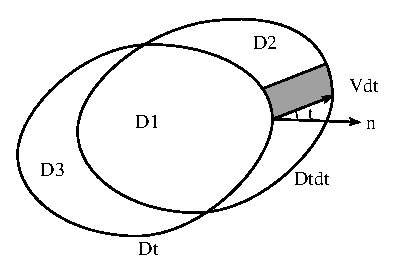
\includegraphics[scale=1]{../images/T1_Ch01-0002.eps}
\end{center}
\end{multicols}

Posant $J(t)=\iiint_{D(t)} \mathcal{A}(x,t) \ud v$, on peut écrire:
\begin{equation*}
    \begin{aligned}
        J(t+\ud t)-J(t) & =\iiint_{D(t+\ud t)} \mathcal{A}(x,t+\ud t) \ud v-\iiint_{D(t)} \mathcal{A}(x,t) \ud v\\
                        & =\iiint_{D_I} \left[\mathcal{A}(x,t+\ud t)-\mathcal{A}(x,t)\right] \ud v+\iiint_{D_{II}} \mathcal{A}(x,t+\ud t) \ud v-\iiint_{D_{III}} \mathcal{A}(x,t) \ud v\\
                        & =\left[\iiint_{D} \frac{\partial \mathcal{A}}{\partial t}(x,t) \ud v\right]\ud t+ \left[\iint_{\partial D} \mathcal{A}\vec{V}\cdot\vec{n} \ud s\right]\ud t
    \end{aligned}
\end{equation*}
en remarquant que pour $II$ ou $III$, l'élément de volume $\ud v$ (hachuré sur la figure ci-contre) est donné par:
\begin{equation*}
    \ud v=\pm V \ud t \cdot \ud S \cdot \cos\theta = \pm \vec{V}\cdot\vec{n} \ud S \ud t
\end{equation*}
On trouvera des démonstrations plus détaillées et plus rigoureuses dans \cite{Germain-62,Germain-73,Mandel-66,Gontier-69} entre autres.

En utilisant le théorème de la divergence (Annexe~\ref{Ann:A}) et la formule donnant la dérivée particulaire $\mathcal{A}$:
\begin{equation*}
    \frac{\ud \mathcal{A}}{\ud t}=\frac{\partial \mathcal{A}}{\partial t}+\mathcal{A}_{,i}V_i
\end{equation*}
(où on a utilisé la convention de sommation et la notation $f_{,i}=\partial f/\partial x_i$ -- voir Annexe~\ref{Ann:A}), on peut transformer~\eqref{eq:Ch01-005} en:
\begin{equation}
    \frac{\ud}{\ud t}\iiint_{D} \mathcal{A} \ud v=\iiint_{D}\left\{\frac{\partial\mathcal{A}}{\partial t}+(\mathcal{A}V_i)_{,i}\right\} \ud v=\iiint_{D} \left\{\frac{\ud\mathcal{A}}{\ud t}+\mathcal{A}\dive\vec{V}\right\} \ud v
    \label{eq:Ch01-006}
\end{equation}
Par une hypothèse analogue au Postulat de Cauchy, on suppose que la densité surfacique $\alpha$ dépend uniquement du point considéré et de la normale $\vec{n}$: $\alpha(M,\vec{n})$.
Moyennant des hypothèses de continuité que nous ne préciserons pas davantage, on montre alors:

\begin{lem}[]
    \hfill
    \begin{enumerate}[(a)]
        \item $\alpha(M,-\vec{n}) =-\alpha(M,\vec{n})$
        \item En un point donné $M$, il existe un flux $\vec{a}(M)$ tel que:
        \begin{equation}
            \alpha(M,\vec{n}) =a_i(M)n_i=\vec{a}\cdot\vec{n}
            \label{eq:Ch01-007}
        \end{equation}
    \end{enumerate}
    \label{lem:Ch01-2}
\end{lem}

\begin{wrapfigure}[3]{l}{.2\textwidth}
    \vskip-1.5em
    \centering
    \psfrag{dS}{\scriptsize $\ud S$}
    \psfrag{n}{\scriptsize $\vec n$}
    \psfrag{-n}{\scriptsize $-\vec n$}
    \psfrag{e}{\scriptsize $\varepsilon$}
    
\includegraphics[clip]{../images/T1_Ch01-0003.eps}%\vspace{.2cm}
\end{wrapfigure}
\noindent Le point a) exprime simplement que ce qui rentre dans $D$ est l'opposé de ce qui en sort.
Lorsque $\varepsilon\rightarrow 0$, les seuls termes qui subsistent sont ceux relatifs aux deux faces, et \eqref{eq:Ch01-004} donne le point a).
\vspace{1em}

\begin{wrapfigure}[5]{r}{.2\textwidth}
    \vskip-2em
    \centering
    \psfrag{x1}{\scriptsize $x_1$}
    \psfrag{x2}{\scriptsize $x_2$}
    \psfrag{x3}{\scriptsize $x_3$}
    \psfrag{M0}{\scriptsize $M_0$}
    \psfrag{M1}{\scriptsize $M_1$}
    \psfrag{M2}{\scriptsize $M_2$}
    \psfrag{M3}{\scriptsize $M_3$}
    \psfrag{-e1}{\scriptsize $-\vec e_1$}
    \psfrag{-e2}{\scriptsize $-\vec e_2$}
    \psfrag{-e3}{\scriptsize $-\vec e_3$}
    \psfrag{n}{\scriptsize $\vec n$}
    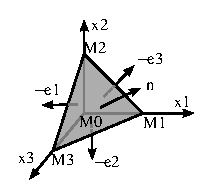
\includegraphics[clip]{../images/T1_Ch01-0004.eps}
\end{wrapfigure}
\noindent Pour démontrer le point b), on écrit~\eqref{eq:Ch01-004} pour un domaine $D$ en forme de tétraèdre $M_OM_1M_2M_3$, la face $M_1M_2M_3$ restant perpendiculaire au vecteur $\vec{n}$ donné.
Lorsque les dimensions du tétraèdre tendent vers zéro, la fonction $\alpha(M,\vec{n})$ reste à peu près constante en et ne dépend donc que de $\vec{n}$.

De plus, seule subsiste dans \eqref{eq:Ch01-004} l'intégrale de surface:
\begin{equation*}
    0=\iint_{M_1M_2M_3}\alpha(\vec{n}) \ud S+\iint_{M_0M_1M_2}\alpha(-\vec{e}_3) \ud S+ \iint_{M_0M_1M_3}\alpha(-\vec{e}_2) \ud S+\iint_{M_0M_2M_3}\alpha(-\vec{e}_1) \ud S
\end{equation*}
Si on note $S$ la surface de la face $M_1M_2M_3$ et $S_1$, $S_2$, $S_3$ celles de $M_OM_2M_3$, $M_OM_1M_3$, $M_0M_1M_2$ respectivement, il vient:
\begin{equation*}
    0 = \alpha(\vec{n})S+\alpha(-\vec{e}_3)S_3+\alpha(-\vec{e}_2)S_2+\alpha(-\vec{e}_1)S_1
\end{equation*}
soit, en utilisant a), en posant $a_i=\alpha(\vec{e}_i)$ et en remarquant que $S_i=\cos(\vec{e}_i,\vec{n})S=n_iS$:
\begin{equation*}
    \alpha(\vec{n})=a_in_i
\end{equation*}
Par utilisation de ces deux lemmes, on obtient la forme locale ou différentielle de la loi de conservation~\eqref{eq:Ch01-004}:
\begin{thm}
    \begin{equation}
        \frac{\ud \mathcal{A}}{\ud t} = -\mathcal{A}V_{i,i} + a_{i,i} + A
        \label{eq:Ch01-008}
    \end{equation}
    \label{thm:Ch01-1}
\end{thm}
\begin{proof}[Première démonstration]
    On utilise le théorème de la divergence pour transformer dans \eqref{eq:Ch01-004} l'intégrale de surface.
    Il vient:
    \begin{equation*}
        \iiint_D\left(\frac{\ud \mathcal{A}}{\ud t}+\mathcal{A}_{i,i}-a_{i,i}-A\right)\ud v=0
    \end{equation*}
    Cette égalité devant avoir lieu pour tout domaine $D$, on en tire la nullité de la quantité intégrée.
\end{proof}

\begin{proof}[Deuxième démonstration]
    On écrit la loi de conservation \eqref{eq:Ch01-004} en choisissant comme domaine $D$ un petit parallélépipède de côtés $h_1$, $h_2$, $h_3$.
    En utilisant le \tmp{lemme X}, on obtient en première approximation:
    \begin{align*}
        \frac{\ud}{\ud t}\iiint_D \mathcal{A} \ud v &= \iiint_D\left(\frac{\ud \mathcal{A}}{\ud t}+\mathcal{A}\dive \vec{V}\right)\ud v \\
        & \simeq \left(\frac{\ud \mathcal{A}}{\ud t}+\mathcal{A}\dive \vec{V}\right) h_1h_2h_3
    \end{align*}
    avec l'hypothèse $\iiint_D A \ud v =A h_1h_2h_3$.

    Pour l'intégrale de surface, on obtient:
    \begin{align*}
        \iint_{\partial D}\alpha \ud S & =\iint_{\partial D}\left(a_1n_1+a_2n_2+a_3n_3\right)\ud S \\
                                       & =\iint_{S_1}\quad \cdots \text{ permutation circulaire}\\
                                       & =\iint_{S_1} \left[a_1(x_1+h_1)-a_1(x_1)\right] \ud x_1 \ud x_2 + \cdots
    \end{align*}
    puisque $\vec{n}= (1,0,0)$ sur $S_1(x_1+h_1)$ et $\vec{n} = (-1,0,0)$ sur $S_1(x_1)$.
    Finalement il vient:
    \begin{equation*}
        \iint_{\partial D}\alpha \ud S=\left(\frac{\partial a_1}{\partial x_1}h_1\right)h_2h_3+\cdots=\frac{\partial a_i}{\partial x_i}h_1 h_2 h_3
    \end{equation*}
    d'où le résultat.
\end{proof}
\rput(11.8,8.5){%
\psfrag{x1}{\scriptsize $x_1$}
\psfrag{x2}{\scriptsize $x_2$}
\psfrag{x3}{\scriptsize $x_3$}
\psfrag{h1}{\scriptsize $h_1$}
\psfrag{h2}{\scriptsize $h_2$}
\psfrag{h3}{\scriptsize $h_3$}
\psfrag{e1}{\scriptsize $\vec e_1$}
\psfrag{e2}{\scriptsize $\vec e_2$}
\psfrag{e3}{\scriptsize $\vec e_3$}
\psfrag{-e1}{\scriptsize $-\vec e_1$}
\psfrag{-e2}{\scriptsize $-\vec e_2$}
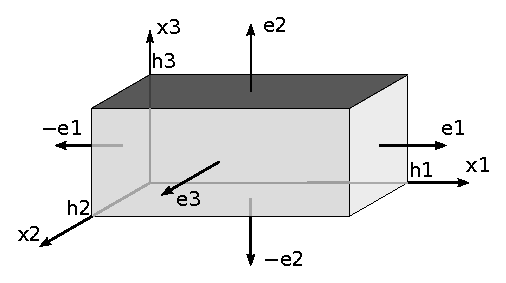
\includegraphics[width=7cm]{../images/T1_Ch01-0005.eps}}
Cette forme locale suppose la continuité des différentes quantités en cause.
En présence d'une surface de discontinuité $\Sigma$ se déplaçant à la vitesse $\vec{V}$, on définit la vitesse relative du choc $U$ par:
\begin{equation}
    U=(\vec{W}-\vec{V})\cdot \vec{N}
    \label{eq:Ch01-009}
\end{equation}
\begin{wrapfigure}[7]{l}{.3\textwidth}
    \psfrag{D}{\scriptsize $D$}
    \psfrag{S}{\scriptsize $\Sigma$}
    \psfrag{W}{\scriptsize $\vec W$}
    \psfrag{N}{\scriptsize $\vec N$}
    \includegraphics{../images/T1_Ch01-0006}
\end{wrapfigure}
On peut alors montrer (voir \cite{Germain-73}) que l'équation locale~\eqref{eq:Ch01-008} doit être complétée par une «~équation aux discontinuités~»:
\begin{equation}
    \llbracket\mathcal{A}U + a_iN_i\rrbracket = 0 
    \label{eq:Ch01-010}
\end{equation}
en désignant par $\llbracket h \rrbracket h(M^+)-h(M^-)$ le saut d'une grandeur à travers $\Sigma$.

L'application du Théorème~\ref{thm:Ch01-1} à la loi de conservation de la masse~\eqref{eq:Ch01-001} donne:
\begin{equation}
    \frac{\ud \rho}{\ud t}+\rho \dive \vec{V}=0
    \label{eq:Ch01-011}
\end{equation}
c'est l'équation de continuité.
Un calcul simple montre alors que:
\begin{equation*}
    \frac{\ud\mathcal{A}}{\ud t}+\mathcal{A}\dive \vec{V}=\rho\left\{\frac{1}{\rho}\frac{\ud \mathcal{A}}{\ud t}-\frac{1}{\rho^2}\mathcal{A}\frac{\ud \rho}{\ud t}\right\}=\rho \frac{\ud}{\ud t}\left(\frac{\mathcal{A}}{\rho}\right)
\end{equation*}
Le Lemme~\ref{lem:Ch01-1} et le Théorème~\ref{thm:Ch01-1} deviennent alors:
\begin{lem}[Lemme 1']
    \begin{equation}
        \frac{\ud}{\ud t}\iiint_D\mathcal{A}\ud v=\iiint_D\rho\frac{\ud}{\ud t}\left(\frac{\mathcal{A}}{\rho}\right)(12)
        \label{eq:Ch01-012}
    \end{equation}
    \label{lem:Ch01-1p}
\end{lem}
\theoremstyle{thm}
\begin{thm}[Théorème 1']
    \begin{equation}
        \rho\frac{\ud}{\ud t}\left(\frac{\mathcal{A}}{\rho}\right)=A+a_{i,i}(13)
        \label{eq:Ch01-013}
    \end{equation}
    \label{thm:Ch01-1p}
\end{thm}
Ces deux formes sont très utiles, car les quantités physiques sont plus souvent définies par leur densité massique $\mathcal{A}/\rho$ que volumique $\mathcal{A}$.
\subsection{Utilisation de la loi fondamentale} \label{ssec:Ch01-1.3}
L'application du Lemme~\ref{lem:Ch01-2} à la loi de conservation de la quantité de mouvement~\eqref{eq:Ch01-002} (en prenant $\alpha=T_i$ permet d'introduire le \emph{tenseur des contraintes} $\sigma_{ij}$
système de 9 quantités, tel que:
\begin{equation}
    T_i=\sigma_{ij}n_j
    \label{eq:Ch01-014}
\end{equation}
Le chapitre~\ref{chap:Ch02} sera consacré à l'étude de ce «~tenseur des contraintes~».

L'application du Théorème~\ref{thm:Ch01-1p} à la loi de conservation de la quantité de mouvement \eqref{eq:Ch01-002} donne alors \emph{l'équation du mouvement}:
\begin{equation}
    \rho\gamma_i=\rho\frac{\ud V_i}{\ud t}=\sigma_{ij,j}+f_i
    \label{eq:Ch01-015}
\end{equation}
où $\gamma_i$ désigne l'accélération:
\begin{equation}
    \gamma_i=\frac{\ud V_i}{\ud t}=\frac{\partial V_i}{\partial t}+V_{i,j}V_j
    \label{eq:Ch01-016}
\end{equation}
Dans la suite de ce cours, on s'intéressera essentiellement aux problèmes statiques.
L'équation du mouvement~\eqref{eq:Ch01-015} devient alors \emph{l'équation d'équilibre}:
\begin{equation}
    \sigma_{ij,j}+f_i=0
    \label{eq:Ch01-017}
\end{equation}
système de 3 équations scalaires ($i=1,2,3$):
\begin{equation}
    \begin{aligned}
        &\frac{\partial \sigma_{11}}{\partial x_1}+\frac{\partial \sigma_{12}}{\partial x_2}+\frac{\partial \sigma_{13}}{\partial x_3}+f_1=0\\
        &\frac{\partial \sigma_{21}}{\partial x_1}+\frac{\partial \sigma_{22}}{\partial x_2}+\frac{\partial \sigma_{23}}{\partial x_3}+f_2=0\\
        &\frac{\partial \sigma_{31}}{\partial x_1}+\frac{\partial \sigma_{32}}{\partial x_2}+\frac{\partial \sigma_{33}}{\partial x_3}+f_3=0
    \end{aligned}
    \label{eq:Ch01-018}
\end{equation}
qui traduisent localement l'équilibre du milieu continu.

La loi de conservation du moment cinétique s'étudie de la même manière: on applique le Théorème~\ref{thm:Ch01-1p} avec $\mathcal{A}/\rho=\varepsilon_{ijk}a_jV_k$, $\alpha=\varepsilon_{ijk}x_jT_k=\varepsilon_{ijk}x_j\sigma_{kl}n_l$ d'après \eqref{eq:Ch01-014}, et $A=\varepsilon_{ijk}x_jk_k$.
Il vient:
\begin{equation*}
    \rho \frac{\ud}{\ud t}(\varepsilon_{ijk}x_jV_k)=(\varepsilon_{ijk}x_j\sigma_{kl})_{,l}+\varepsilon_{ijk}x_jf_k
\end{equation*}
On développe cette relation en remarquant que:
\begin{equation*}
    \frac{\ud x_j}{\ud t}=V_j, \qquad x_{j,l}=\frac{\partial x_j}{\partial x_l}=\delta_{jl}
\end{equation*}
où $\delta_{jl}$ est le symbole de Kronecker:
\begin{equation*}
    \rho \varepsilon_{ijk}V_jV_k+\rho\varepsilon_{ijk}x_j\gamma_k=\varepsilon_{ijk}\delta_{jl}\sigma_{kl}+\varepsilon_{ijk}x_j\sigma_{kl,l}+ \varepsilon_{ijk}x_jf_k
\end{equation*}
Le premier terme disparaît car $\varepsilon_{ijk}$ est antisymétrique en $j$ et $k$.
Il reste:
\begin{equation*} 
    \varepsilon_{ijk}x_j(\rho\gamma_k-\sigma_{kl,l}-f_k)-\varepsilon_{ijk}\sigma_{jk}=0
\end{equation*}
Le premier terme s'annule d'après \eqref{eq:Ch01-015} et on obtient finalement $\varepsilon_{ijk}\sigma_{jk}=0$ c'est à dire:
\begin{equation}
    \sigma_{ij}=\sigma_{ji}
    \label{eq:Ch01-019}
\end{equation}
Le tenseur des contraintes est symétrique.
\begin{displaymath}
    \sigma_{12} = \sigma_{21}, \quad \sigma_{13}= \sigma_{31}, \quad \sigma_{23} = \sigma_{32}
\end{displaymath}
Ainsi la loi fondamentale de la dynamique est, sous forme locale, équivalente â l'équation du mouvement~\eqref{eq:Ch01-015} avec un tenseur des contraintes symétrique.
A nouveau ces résultats supposent la continuité des fonctions en cause.
En présence d'une surface de discontinuité $\Sigma$, il faut rajouter les relations de discontinuité \eqref{eq:Ch01-010} qui donnent:
\begin{itemize}
     \item pour la conservation de la masse:
        \begin{equation}
            \llbracket \rho U \rrbracket=0, \qquad \rho^+(\vec{W}-\vec{V}^+)\cdot \vec{N} =\rho^-(\vec{W}-\vec{V}^-)\cdot \vec{N}
            \label{eq:Ch01-020}
        \end{equation}
    \item pour la conservation de la quantité de mouvement:
    \begin{equation}
        \llbracket \rho U V_i +\sigma_{ij}N_j \rrbracket=0
        \label{eq:Ch01-021}
    \end{equation}
\end{itemize}
tandis que l'équation correspondante pour la conservation du moment cinétique est automatiquement vérifiée si \eqref{eq:Ch01-022} l'est.

Dans le cas statique, ces relations de discontinuité se ramènent à la seule condition:
\begin{equation}
    \llbracket\sigma_{ij}N_j\rrbracket=0,\qquad \vec{T}^+(\vec{N})=\vec{T}^-(\vec{N})
    \label{eq:Ch01-022}
\end{equation}
exprimant la continuité du vecteur $\vec{T}$.
Nous y reviendrons au chapitre~\ref{chap:Ch02}.
\section{Puissances virtuelles} \label{sec:Ch01-2}
\subsection{Théorème des puissances virtuelles} \label{ssec:Ch01-2.1}
Pour un système quelconque un mouvement virtuel est un mouvement possible de ce système mouvement «~virtuel~» par opposition au mouvement «~réel~» qui est celui qui se réalise effectivement par suite des efforts appliqués.
De même une «~vitesse virtuelle~» est une répartition de vitesse possible.
Pour un milieu continu déformable, une vitesse virtuelle sera définie par un champ de vitesses virtuelles $\displaystyle{\mathop{V}^{*}}_i(x)$, c'est à dire par un champ de vecteurs $\displaystyle{\mathop{V}^{*}}_i$ défini sur le solide $\Omega$.

Nous partons donc de l'équation du mouvement~\eqref{eq:Ch01-015} que nous multiplions par $\displaystyle{\mathop{V}^{*}}_i$ (il s'agit donc d'un produit scalaire), et nous intégrons sur le solide $\Omega$ tout entier:
\begin{equation*}
    \iiint_{\Omega}\rho\gamma_i {\mathop{V}^{*}}_i \ud v=\iiint_{\Omega}\sigma_{ij,j} {\mathop{V}^{*}}_i \ud v+\iiint_{\Omega}f_i {\mathop{V}^{*}}_i \ud v
\end{equation*}
mais en utilisant le
\begin{thm}[théorème de la divergence]
\begin{align*}
    \iiint_{\Omega}\sigma_{ij,j} {\mathop{V}^{*}}_i \ud v &= \iiint_{\Omega}[(\sigma_{ij} {\mathop{V}^{*}}_i)_{,j}-\sigma_{ij} {\mathop{V}^{*}}_{i,j}]\ud v\\
    &=\iint_{\partial \Omega}\sigma_{ij} {\mathop{V}^{*}}_i n_j \ud S-\iiint_{\Omega} \sigma_{ij} {\mathop{V}^{*}}_{i,j} \ud v
\end{align*}
\end{thm}
Grâce à \eqref{eq:Ch01-014}, on retrouve dans le premier terme les efforts $\vec{T}$ appliqués sur $\Omega$ à travers $\partial \Omega$, tandis que, d'après la symétrie de $\sigma_{ij}$, on peut remplacer $\displaystyle{\mathop{V}^{*}}_{i,j}$ par sa partie symétrique $\displaystyle{\mathop{D}^{*}}_{ij}$ (Annexe~\ref{Ann:A}):
\begin{equation}
    {\mathop{V}^{{\ast}}}_{i,j}={\mathop{D}^{{\ast}}}_{ij}+{\mathop{\Omega}^{{\ast}}}_{ij},\qquad
    {\mathop{D}^{{\ast}}}_{ij}={\mathop{V}^{{\ast}}}_{i,j}+{\mathop{V}^{{\ast}}}_{j,i},\qquad
    {\mathop{\Omega}^{{\ast}}}_{ij}={\mathop{V}^{{\ast}}}_{i,j}-{\mathop{V}^{{\ast}}}_{j,i}
    \label{eq:Ch01-023}
\end{equation}
$\displaystyle{\mathop{D}^{{\ast}}}_{ij}$ est le tenseur taux de déformation et $\displaystyle{\mathop{\Omega}^{{\ast}}}_{ij}$ le tenseur au champ de vitesses virtuelles $\displaystyle{\mathop{V}^{{\ast}}}_i$.
Finalement on obtient:
\begin{equation}
    \everymath{\displaystyle}
    \begin{array}{cccc}
        \iiint_{\Omega}\rho\gamma_i {\mathop{V}^{\ast}}_i \ud v & = \iiint_{\Omega}f_i {\mathop{V}^{\ast}}_i \ud v & +                                                    \iint_{\partial\Omega}T_i {\mathop{V}^{\ast}}_i \ud S & -                           \iiint_{\Omega}\sigma_{ij} {\mathop{D}^{\ast}}_{ij} \ud v\\[7pt]
        \mathop{\mathcal{P}}^{\ast}{\!}^{(\text{a})} & = \mathop{\mathcal{P}}^{\ast}{\!}^{(\text{d})} & + \mathop{\mathcal{P}}^{\ast}{\!}^{(\text{c})} & + \mathop{\mathcal{P}}^{\ast}{\!}^{(\text{int})}\\[7pt]
        & =  & \mathop{\mathcal{P}}^{\ast}{\!}^{(\text{ext})} & + \mathop{\mathcal{P}}^{\ast}{\!}^{(\text{int})}
    \end{array}
    \label{eq:Ch01-024}
\end{equation}
en introduisant:
\begin{itemize}
    \item $\displaystyle \mathop{\mathcal{P}}^{\ast}{\!}^{(\text{a})}$: Puissance virtuelle des quantités d'accélération dans le champ de vitesses virtuelles $\displaystyle\mathop{V}^{\ast}$;
    \item $\displaystyle \mathop{\mathcal{P}}^{\ast}{\!}^{(\text{d})}$: Puissance virtuelle des efforts à distance;
    \item $\displaystyle \mathop{\mathcal{P}}^{\ast}{\!}^{(\text{c})}$: Puissance virtuelle des efforts à contact;
    \item $\displaystyle \mathop{\mathcal{P}}^{\ast}{\!}^{(\text{ext})} = \mathop{P}^{\ast}{\!}^{(\text{d})} + \mathop{P}^{\ast}{\!}^{(\text{c})}$: Puissance virtuelle des efforts extérieurs.
\end{itemize}
On retrouve donc l'énoncé classique des puissances virtuelles, à condition d'interpréter le terme complémentaire $\displaystyle \mathop{\mathcal{P}}^{\ast}{\!}^{(\text{int})}$ comme étant la puissance virtuelle des efforts intérieurs:
\begin{equation}
    \mathop{\mathcal{P}}^{\ast}{\!}^{(\text{int})}=-\iiint_\Omega \sigma_{ij}{\mathop{\mathcal{D}}^{\ast}}_{ij} \ud v
    \label{eq:Ch01-025}
\end{equation}
On peut s'assurer (voir \cite{Germain-62,Gontier-69}) que c'est une interprétation justifiée dans la mesure où elle généralise la puissance virtuelle des efforts intérieurs introduite en mécanique rationnelle pour un système de solides rigides.
En particulier, le lemme suivant montre que la puissance virtuelle des efforts intérieurs est nulle dans tout champ de vitesses rigidifiant, c'est à dire lorsque $\displaystyle {\mathop{V}^{\ast}}_i$ est le champ de vitesses d'un solide rigide. 

\begin{lem}
    Une condition nécessaire et suffisante pour qu'un champ de vitesses $\displaystyle {\mathop{V}^{\ast}}_i$ soit rigidifiant est que le tenseur taux de déformation associé $\displaystyle {\mathop{D}^{\ast}}_{ij}$ soit nul.
    \label{lem:Ch01-3}
\end{lem}
\begin{proof}
    \begin{description}
        \item[Condition nécessaire.] Un champ rigidifiant peut s'écrire 
            \begin{equation}
                \mathop{V}^{\ast}(M) = \vec{a} + \vec{b} \wedge \vec{OM},\quad {\mathop{V}^{\ast}}_i = a_i + \varepsilon_{ijk} b_j x_k
                \label{eq:Ch01-026}
            \end{equation}
            On obient alors directement
            \begin{displaymath}
                {\mathop{V}^{\ast}}_{i,j} = \varepsilon_{ijl}b_k = {\mathop{\Omega}^{\ast}}_{ij},\quad {\mathop{D}^{\ast}}_{ij} = 0
            \end{displaymath}
        \item[Condition suffisante.] Il faut montrer que la condition
            \begin{equation}
                {\mathop{D}^{\ast}}_{ij} = \frac{1}{2} \left( {\mathop{V}^{\ast}}_{i,j} + {\mathop{V}^{\ast}}_{j,i} \right) = 0
                \label{eq:Ch01-027}
            \end{equation}
            permet d'écrire~\eqref{eq:Ch01-026}.
            Nous démonstrerons ce résultat au chapitre~\ref{chap:Ch03} (paragraphe~\ref{ssec:Ch01-3.1}, Théorème~\ref{thm:Ch03-2}).
    \end{description}
\end{proof}
Nous avons donc démontré, à partir de la loi fondamentale, le
\newtheorem*{TPV}{Théorème des puissances virtuelles}
\begin{TPV}
    Dans tout mouvement virtuel, la puissance virtuelle des quantités d'accélération est égale à la puissance virtuelle des efforts extérieurs et intérieurs
    \begin{equation}
        \mathop{\mathcal{P}}^{\ast}{\!}^{(\text{a})} = \mathop{\mathcal{P}}^{\ast}{\!}^{(\text{ext})} + \mathop{\mathcal{P}}^{\ast}{\!}^{(\text{int})}
        \label{eq:Ch01-028}
    \end{equation}
\end{TPV}

En particulier, si on prend comme champ de vitesses le champ des vitesse réelles, on obtien le
\newtheorem*{TEC}{Théorème de l'énergie cinétique}
\begin{TEC}
    La dérivée par rapport au temps de l'énergie cinétique est égale à la puissance des efforts extérieurs et intérieurs
    \begin{align}
        \frac{\ud}{\ud t}\left( \frac{1}{2}\iiint_{\Omega} \rho V_iV_i \ud v\right) &= \iiint_{\Omega} f_i V_i \ud v &+ \iint_{\partial\Omega} T_i V_i \ud S &- \iiint_{\Omega} \sigma_{ij} D_ij \ud v \nonumber\\
        \frac{\ud K}{\ud t} &= \mathop{\mathcal{P}}^{\ast}{\!}^{(\text{ext})} &&+ \mathop{\mathcal{P}}^{\ast}{\!}^{(\text{int})}
        \label{eq:Ch01-029}
    \end{align}
\end{TEC}
\subsection{Le principe des puissances virtuelles} \label{ssec:Ch01-2.2}
Dans le cours de Mécanique Analytique, on a vu que l'on pouvait reconstruire la mécanique d'un système de solides à partir de l'énoncé des puissances virtuelles pris comme loi physique de départ.
La loi fondamentale est alors obtenue comme conséquence.
L'idée de départ est de caractériser un système d'efforts non plus par une densité volumique, surfacique ou autre, mais par la puissance que ce système d'efforts développe dans un mouvement virtuel quelconque.
En d'autres termes, un système d'efforts est une forme linéaire sur l'espace des vitesses virtuelles.
L'espace des efforts est donc dual de l'espace des vitesses virtuelles.

Nous postulons donc
\newtheorem*{PPV}{Principe des puissances virtuelles}
\begin{PPV}
    La puissance virtuelle des quantités d'accélération est égale à la puissance virtuelle des efforts intérieurs et extérieurs
    \begin{equation}
        \mathop{\mathcal{P}}^{\ast}{\!}^{(a)} = \mathop{\mathcal{P}}^{\ast}{\!}^{(ext)} + \mathop{\mathcal{P}}^{\ast}{\!}^{(int)}
        \label{eq:Ch01-030}
    \end{equation}
    dans tout mouvement virtuel.
\end{PPV}


Toutes ces puissances virtuelles sont des formes linéaires sur l'espace $\mathop{\mathcal{V}}^{\ast}$ des champs de vitesses virtuelles:
\begin{itemize}
    \item La puissance des quantités d'accélération, $\mathop{\mathcal{P}}^{\ast}{\!}^{(a)}$, est imposée par le type de cinématique que l'on envisage.
    \item La puissance des efforts extérieurs, qui se décompose en deux parties:
        \begin{equation}
            \mathop{\mathcal{P}}^{\ast}{\!}^{(ext)} = \mathop{\mathcal{P}}^{\ast}{\!}^{(a)} + \mathop{\mathcal{P}}^{\ast}{\!}^{(c)}
            \label{eq:Ch01-031}
        \end{equation}
        (la puissance des efforts à distance $\mathop{\mathcal{P}}^{\ast}{\!}^{(d)}$ et la puissance des efforts de contact $\mathop{\mathcal{P}}^{\ast}{\!}^{(c)}$) est imposée par la nature des efforts extérieurs (donc connus) appliqués.
    \item La puissance des efforts intérieurs, par contre, pose davantage de problèmes:\\
        on sait que
        \newtheorem*{AXM}{Axiome}
        \begin{AXM}
            La puissance virtuelle des efforts intérieurs est nulle dans tout mouvement rigidifiant.
        \end{AXM}
\end{itemize}

Construire une théorie des milieux continus, c'est d'abord choisir l'espace $\mathop{\mathcal{V}}^{\ast}$ des champs de vitesses virtuelles, c'est ensuite choisir la forme des quatre formes linéaires $\mathop{\mathcal{P}}^{\ast}{\!}^{(a)}$, $\mathop{\mathcal{P}}^{\ast}{\!}^{(d)}$, $\mathop{\mathcal{P}}^{\ast}{\!}^{(c)}$ et $\mathop{\mathcal{P}}^{\ast}{\!}^{(int)}$.
Le reste de la théorie -- donc en particulier les équations du mouvement -- s'obtiennent par des calculs simples.

Considérons par exemple le cas de la mécanique des solides rigides: l'espace $\mathop{\mathcal{V}}^{\ast}$ des vitesses virtuelles est l'espace des champs de vitesses d'un solide, espace vectoriel de dimension 6.
Les formes linéaires $\mathop{\mathcal{P}}^{\ast}{\!}^{(a)}$ et $\mathop{\mathcal{P}}^{\ast}{\!}^{(ext)}$ (d'après l'axiome, $\mathop{\mathcal{P}}^{\ast}{\!}^{(int)}$ identiquement nulle) sont donc des éléments du dual de cet espace: l'espace des «~torseurs~».
Le principe des puissances virtuelles est donc équivalent à la loi fondamentale
\begin{equation}
    \left[ \mathcal{A} \right] = \left[ \mathcal{F}^{(ext)} \right]
    \label{eq:Ch01-032}
\end{equation}
où $\left[ \mathcal{A} \right]$ est le torseur des quantités d'accélération et $\left[ \mathcal{F}^{(ext)} \right]$ le torseur des efforts extérieurs.

De manière générale, la mécanique des milieux continus peut être construite indifféremment à partir des lois de conservation, comme nous l'avons fait au paragraphe~\ref{ssec:Ch01-1.1}, ou à partir du principe des puissances virtuelles, comme nous le ferons au paragraphe~\ref{ssec:Ch01-2.3}.
L'approche des puissances virtuelles présente cependant un double avantage:
\begin{enumerate}
    \item Elle est beaucoup plus systématique, et permet donc une généralisation plus facile lorsque l'on veut sortir du cadre des milieux continus classiques, pour étudier par exemple les milieux avec micro-structure évoqués au paragraphe~\ref{ssec:Ch01-1.1} cas des cristaux liquides ou bien les matériaux électromagnétiques.
    \item Elle met clairement en évidence la relation entre la description cinématique et la schématisation des efforts: plus on raffine la description cinématique, plus il faut raffiner la schématisation des efforts, et réciproquement.
        Par exemple, dans le cas du solide rigide, on voit clairement que la schématisation des efforts par des torseurs est liée à la cinématique du solide rigide: deux répartitions d'efforts différentes conduisant au même torseur sont équivalentes, car elles développent la même puissance dans tout mouvement possible.
\end{enumerate}

Pour ce cours élémentaire, nous ne partirons pas systématiquement de l'approche «~puissances virtuelles~», mais nous la mentionnerons régulièrement, et nous l'utiliserons pour mettre en évidence la dualité contraintes--déformations, ce qui sera une simple vérification en mécanique des milieux continus, mais jouera un rôle essentiel plus tard, en Résistance des Matériaux.

\subsection{Théorie du premier gradient} \label{ssec:Ch01-2.3}
Comme nous l'avons annoncé, nous allons ici reconstruire les équations fondamentales du paragraphe~\ref{ssec:Ch01-1.1} à partir du principe des puissances virtuelles.
En MMC classique, l'espace $\mathop{\mathcal{V}}^{\ast}$ est l'espace des champs de vecteurs sur le domaine $\Omega$ occupé par le solide.
Nous considérons une théorie du premier gradient, c'est à dire nous supposons que dans les formes linéaires définissant les puissances virtuelles, seul intervient le champ des vitesses virtuelles $\mathop{V}^{\ast}_i$ et son premier gradient $\mathop{V}^{\ast}_{i,j}$.

La schématisation des accélérations et des efforts extérieurs est la même que dans l'approche classique.
Nous prenons donc pour la puissance virtuelle des quantités d'accélération et des efforts extérieurs les formes suivantes
\begin{equation}
    \mathop{\mathcal{P}}^{\ast}{\!}^{(a)} = \iiint_{\Omega} \rho \gamma_i \mathop{V}^{\ast}_i \ud v \quad
    \mathop{\mathcal{P}}^{\ast}{\!}^{(d)} = \iiint_{\Omega} f_i \mathop{V}^{\ast}_i \ud v \quad
    \mathop{\mathcal{P}}^{\ast}{\!}^{(c)} = \iint_{\partial\Omega} T_i^e \mathop{V}^{\ast}_i \ud S
    \label{eq:Ch01-33}
\end{equation}
où $\gamma_i$ est l'accélération, $f_i$ les efforts à distance et $T_i^e$ les efforts de contact exercés sur le solide $\Omega$ à travers $\partial \Omega$ (alors que $T_i$ introduit au paragraphe~\ref{ssec:Ch01-1.1} était relatif à un sous-domaine quelconque $D\subset \Omega$: les lois de conservation sont imposées à tout domaine matériel $D$ alors que le principe des puissances virtuelles est écrit globalement pour le solide $\Omega$ tout entier).

La schématisation des efforts intérieurs, par contre, diffère de celle du paragraphe~\ref{ssec:Ch01-1.1} conformément à notre hypothèse d'une théorie du premier gradient, nous prenons
\begin{equation}
    \mathop{\mathcal{P}}^{\ast}{\!}^{(int)} = \iiint_{\Omega} \left( A_i \mathop{V}^{\ast}_i + B_{ij} \mathop{V}^{\ast}_{i,j} \right) \ud v
    \label{eq:Ch01-034}
\end{equation}
où les quantités $A_i$ et $B_{ij}$ caractérisent les efforts intérieurs.
En décomposant le tenseur gradient des vitesses $\mathop{V}^{\ast}_{i,j}$ en partie symétrique et antisymétrique, conformément à \eqref{eq:Ch01-023}, on peut remplacer \eqref{eq:Ch01-034} par
\begin{equation}
    \mathop{\mathcal{P}}^{\ast}{\!}^{(int)} = \iiint_{\Omega} \left( A_i \mathop{V}^{\ast}_i + \chi_{ij} \mathop{\Omega}^{\ast}_{ij} - \sigma_{ij} \mathop{D}^{\ast}_{ij} \right) \ud v
    \label{eq:Ch01-035} 
\end{equation}<++>
avec $\sigma_{ij}$ symétrique et $\chi_{ij}$ antisymétrique.
D'autre part, on a vu (démonstration du Lemme~\ref{lem:Ch01-3}) que dans un mouvement rigidifiant on avait
\begin{equation}
    \mathop{V}^{\ast}_i = a_i \text{qcq}, \quad \tmp{\varepsilon_i k_j b_k \text{qcq}, \quad \mathop{I}^{\ast}_ij = 0}
    \label{eq:Ch01-036}
\end{equation}
L'axiome du paragraphe~\ref{ssec:Ch01-2.2} montre alors que $A_i$ et $\chi_{ij}$ doivent être nuls.
Il reste
\begin{equation}
    \mathop{\mathcal{P}}^{\ast}{\!}^{(int)} = -\iiint_{\Omega} \sigma_{ij} \mathop{D}^{\ast}_{ij} \ud v
    \label{eq:Ch01-037}
\end{equation}
Les efforts intérieurs sont donc caractérisés par un tenseur symétrique $\sigma_{ij}$.
Nous obtenons donc 
\newtheorem*{PPVMMC}{Principe des puissances virtuelles en MMC}
\begin{PPVMMC}
    \begin{equation}
        \iiint_{\Omega} \rho \gamma_i \mathop{V}^{\ast}_i \ud v = \iiint_{\Omega} f_i \mathop{V}^{\ast}_i \ud v + \iint_{\partial \Omega} T_i^e \mathop{V}^{\ast}_i \ud S - \iiint_{\Omega} \sigma_{ij} \mathop{D}^{\ast}_{ij} \ud v
        \label{eq:Ch01-038}
    \end{equation}
    pour tout champ de vitesses virtuelles $\mathop{V}^{\ast}_i$.
\end{PPVMMC}

Pour utiliser ce principe, il suffit maintenant de reprendre à l'envers le calcul du paragraphe~\ref{ssec:Ch01-3.1}:
\begin{align*}
    \iiint_{\Omega} \sigma_{ij} \mathop{D}^{\ast}_{ij} \ud v &= \iiint_{\Omega} \sigma_{ij} \mathop{V}^{\ast}_{i,j} \\
    &= \iint_{\partial \Omega} \sigma_{ij} \mathop{V}^{\ast}_{i} n_j \ud S - \iiint_{\Omega} \sigma_{ij,j} \mathop{V}^{\ast}_{i} \ud v
\end{align*}
ou l'on a utilisé la symétrie de $\sigma_{ij}$ et le théorème de la divergence.
On obtient alors
\begin{displaymath}
    \iiint_{\Omega} \left( \rho \gamma_i -f_i - \sigma_{ij,j} \right) \mathop{V}^{\ast}_i \ud v + \iint_{\partial \Omega} \left( \sigma_{ij} n_j - T_i^e \right) \mathop{V}^{\ast}_i \ud S = 0
\end{displaymath}
Ceci devant être vrai pour tout champ $\mathop{V}^{\ast}_i$, on en tire l'équation du mouvement \eqref{eq:Ch01-035} et la relation
\begin{equation}
    T_i^e = \sigma_{ij} n_j
    \label{eq:Ch01-039}
\end{equation}
qui est la relation~\eqref{eq:Ch01-014} pour $D=\Omega$. 

\section{Thermodynamique des milieux continus} \label{sec:Ch01-3}
\subsection{Conservation de l'énergie} \label{ssec:Ch01-3.1}
Le premier principe de la thermodynamique affirme que la variation de l'énergie totale (énergie interne + énergie cinétique) est, pour un domaine matériel $D$ quelconque, égale à la somme du travail des efforts extérieurs exercés sur $D$ et de la quantité de chaleur apportée à $D$
\begin{equation}
    \frac{\ud}{\ud t} \left( E + K \right) = \mathcal{P}^{(ext)} + Q
    \label{eq:Ch01-040}
\end{equation}
où 1'énergie cinétique $K$ et la puissance âes efforts extérieurs $\mathcal{P}^{(ext)}$ sont données par
\begin{equation}
    K = \iiint_{D} \frac{1}{2} \rho V_i V_i \ud v
    \label{eq:Ch01-041}
\end{equation}
\begin{equation}
    \mathcal{P}^{(ext)} = \iiint_{D} f_i V_i \ud v + \iint_{\partial D} T_i V_i \ud S
    \label{eq:Ch01-042}
\end{equation}
où l'énergie interne $E$ est définie par
\begin{equation}
    E = \iiint_{D} \rho e \ud v
    \label{eq:Ch01-043}
\end{equation}
en notant $e$ l'énergie interne par unité de masse, et où le taux de chaleur $Q$ apportée à $D$ résulte d'un apport volumique $r$ (rayonnnement) dans $D$ et d'un apport surfacique $h$ (conduction) à travers $\ud D$
\begin{equation}
    Q = \iiint_{D} r \ud v + \iint_{\partial D} h \ud S
    \label{eq:Ch01-044}
\end{equation}
Le premler principe de la thermodynamique conduit donc à la loi de consvation de l'énergie
\begin{equation}
    \frac{\ud}{\ud t} \iiint_D \rho \left( e + \frac{1}{2} V_i V_i \right) \ud v = \iiint_D \left( f_i V_i + r \right) \ud v + \iint_{\partial D} \left( T_i V_i + h \right) \ud S
    \label{eq:Ch01-045}
\end{equation}
qui rentre dans le cadre des lois de conservation définies au paragraphe~\ref{ssec:Ch01-1.1} en prenant
dans~\eqref{eq:Ch01-004}
\begin{table*}
    \centering
    \begin{tabular}[]{c|c|c}
        $\mathcal{A}$ & $\alpha$ & $A$ \\ \hline
        $\rho \left( e \frac{1}{2} V_i V_i \right)$ & $f_i V_i + r$ & $T_i V_i + h$
    \end{tabular}
\end{table*}

Compte-tenu de~\eqref{eq:Ch01-014}, le Lemme~\ref{lem:Ch01-2} du paragraphe~\ref{ssec:Ch01-1.2} permet d'introduire le vecteur flux de chaleur $\vec{q}$ qui permet de décrire les échanges de chaleur à travers $\partial D$ par
\begin{equation}
    h = - \vec{q} \cdot \vec{n} = -q_i n_i
    \label{eq:Ch01-046}
\end{equation}
L'application du Théorème~\ref{thm:Ch01-1p} donne alors
\begin{align*}
    & \rho \left( \frac{\ud e}{\ud t} + V_i \gamma_i \right) = \left( \sigma_{ij} V_i - q_j \right)_{,j} + f_i V_i + r\\
    & \rho \frac{\ud e}{\ud t} + \left( \rho \gamma_i - \sigma_{ij,j} - f_i \right) V_i = \sigma_{ij} V_{i,j} + r - q_{j,j}
\end{align*}
Le terme entre parenthèses disparaît d'après l'équation du mouvement \eqref{eq:Ch01-015}, et, compte-tenu de la symétrie de $\sigma_{ij}$, il reste
\begin{equation}
    \rho \frac{\ud e }{\ud t} = \sigma_{ij} D_{ij} + r - q_{j,j}
    \label{eq:Ch01-047}
\end{equation}
forme  locale du premier principe de la thermodynamique.

On aurait également pu obtenir \eqref{eq:Ch01-047} en utilisant le théorème de l'énergie cinétique du paragraphe~\ref{ssec:Ch01-2.1}.
Ce théorème permet en effet de remplacer \eqref{eq:Ch01-040} par
\begin{equation}
    \frac{\ud E}{\ud t} = Q - \mathcal{P}^{(int)}
    \label{eq:Ch01-048}
\end{equation}
ce  qui, d'après~\eqref{eq:Ch01-025}, donne, au lieu de \eqref{eq:Ch01-045},
\begin{equation}
    \frac{\ud}{\ud t} \iiint_{D} \rho e \ud v = \iiint_{D} \left( \sigma_{ij} D_{ij} + r \right) \ud v + \iint_{\partial D} h \ud S
    \label{eq:Ch01-049}
\end{equation}
et l'application du Lemme~\ref{lem:Ch01-2} et du Théorème~\ref{thm:Ch01-1p} à cette loi de conservation redonne directement \eqref{eq:Ch01-046} et \eqref{eq:Ch01-047}.

On pourrait également écrire l'équation aux discontinuités \eqref{eq:Ch01-010} associée à cette loi de conservation \eqref{eq:Ch01-045}
\begin{equation}
    \llbracket \rho \left( e + \frac{1}{2} V_i V_i \right) U + \left( \sigma_{ij} V_i + q_j \right) N_j \rrbracket = 0
    \label{eq:Ch01-050}
\end{equation}
mais elle sert peu en mécanique des solides.
Remarquons toutefois que l'on n'a pas le droit d'écrire cette relation aux discontinuités sur la loi de conservation~\eqref{eq:Ch01-049}, car on a utilisé pour obtenir~\eqref{eq:Ch01-045} le théorème de l'énergie cinétique, lequel suppose que le champ des vitesses est continu.

\subsection{Inégalité de Clausius-Duhem} \label{ssec:Ch01-3.2}
Le second principe de la thermodynamique qui, en thermostatique, pour un processus homotherme, s'écrit classiquement
\begin{equation}
    \ud S \geq \frac{1}{T} \ud Q
    \label{eq:Ch01-051}
\end{equation}
se généralise habituellement à la MMC sous la forme 
\begin{equation}
    \frac{\ud S}{\ud t} \geq \mathcal{S}^{(ext)} \quad \mathcal{S}^{(int)} = \frac{\ud S}{\ud t} - \mathcal{S}^{(ext)} \geq 0
    \label{eq:Ch01-052}
\end{equation}
exprimant que, pour tout domaine matériel $D$, le taux de ``production interne'' d'entropie $\mathcal{S}^{(int)}$ est positif, la production interne d'entropie étant définie comme étant la différence entre la variation de l'entropie du domaine $D$, définie par
\begin{equation}
    S = \iiint_{D} \rho \eta \ud v
    \label{eq:Ch01-053}
\end{equation}
où $\eta$ est l'entropie par unité de masse, et les ``échanges'' lT dT entropie avec l'extérieur, liés aux échanges de chaleur \eqref{eq:Ch01-044} par
\begin{equation}
    \mathcal{S}^{(ext)} = \iiint_{D} \frac{r}{\theta} \ud v + \iint_{\partial D} \frac{h}{\theta} \ud S
    \label{eq:Ch01-054}
\end{equation}
où $\theta$ est la température absolue.
Ainsi, compte-tenu de \eqref{eq:Ch01-046}, le second principe de la thermodynamique s'écrit sous la forme
\begin{equation}
    \frac{\ud}{\ud t} \iiint_D \rho \eta \ud v \geq \iiint_{D} \frac{r}{\theta} \ud v - \iint_{\partial D} \frac{q_i n_i}{\theta} \ud S
    \label{eq:Ch01-055}
\end{equation}
En utilisant le \tmp{Lemme~\ref{lem:Ch01-2p}} et le théorème de la divergence, on obtient la forme locale du second principe
\begin{align}
        \rho \frac{\ud \eta}{\ud t}  &\geq \frac{r}{\theta} - \left( \frac{q_i}{\theta} \right)_{,i} \nonumber\\
        \rho \theta \frac{\ud \eta}{\ud t}  &\geq r - q_{i,i} + \frac{1}{\theta} q_i\theta_{,i}
    \label{eq:Ch01-056}
\end{align}
En éliminant $r$ entre \eqref{eq:Ch01-047} et \eqref{eq:Ch01-056}, on obtient
\begin{equation}
    -\rho \left( \frac{\ud e}{\ud t} - \theta \frac{\ud \eta}{\ud t} \right) - \frac{1}{\theta}q_i \theta_{,i} + \sigma_{ij}D_{ij} \geq 0
    \label{eq:Ch01-057}
\end{equation}
c'est l'inégalité de Clausius-Duhem, que l'on peut aussi écrire sous la forme
\begin{equation}
    -\rho \left( \frac{\ud \psi}{\ud t} + \eta \frac{\ud \theta}{\ud t} \right) - \frac{1}{\theta}q_i \theta_{,i} + \sigma_{ij}D_{ij} \geq 0
    \label{eq:Ch01-058}
\end{equation}
où $\psi = e -\eta \theta$ est 1'énergie libre par unité de masse.

D'un point de vue purement mécanique, le second principe traduit l'irréversibilité et joue donc un rôle important.
En ``oubliant'' les variables thermiques, on peut réécrire \eqref{eq:Ch01-057} ou \eqref{eq:Ch01-058} sous la forme
\begin{equation}
    \left\{
    \begin{aligned}
        & \phi = -\rho \frac{\ud u}{\ud t} + \sigma_{ij} D_{ij} \geq 0\\
        & \sigma_{ij} D_{ij} = \rho \frac{\ud u}{\ud t} + \phi
    \end{aligned}
    \right.
    \label{eq:Ch01-059}
\end{equation}
où $u$ est l'énergie (interne ou libre, cela n'a plus d'importance, car on a oublié les variables thermiques) du matériau, et où $\phi$ est appelé dissipation.
En reportant dans le théorème de l'énergie cinétique, on obtient 
\begin{equation}
    \mathcal{P}^{(ext)} = \frac{\ud K}{\ud t} + \frac{\ud U}{\ud t} + \Phi^{(irr)} \qquad \Phi^{(irr)} = \iiint_{D} \phi \ud v \geq 0
    \label{eq:Ch01-060}
\end{equation}

La puissance des efforts extérieurs, c'est à dire la puissance dépensée, contribue à augmenter l'énergie cinétique et l'énergie du matériau, et est dissipée dans $\Phi^{(irr)}$.


\chapter{Le tenseur des contraintes} \label{chap:Ch02}
\section{Notions générales} \label{sec:Ch02-1}
\subsection{Vecteur contrainte tenseur des contraintes} \label{ssec:Ch02-1.1}
\begin{multicols}{2}
    \begin{center}
        \psfrag{D}{$D$}
        \psfrag{O}{$\Omega$}
        \psfrag{M1}{$M_1$}
        \psfrag{M2}{$M_2$}
        \psfrag{n}{$\vec{n}$}
        \psfrag{df}{$\vec{\ud f}$}
        \psfrag{T}{$\vec{T}$}
        \psfrag{Tt}{$\vec{T}_t$}
        \psfrag{Tn}{$\vec{T}_n$}
    \includegraphics{../images/T1_Ch02-0001}
    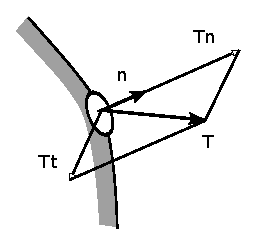
\includegraphics{../images/T1_Ch02-0002}
    \end{center}
\end{multicols}
Le vecteur contrainte caractérise les efforts de contact exercés à travers un élément de surface $\ud S$ de normale $\vec{n}$ sur une partie $D$ du milieu continu: le vecteur contrainte est défini par
\begin{equation}
    \vec{T}(\vec{n}) = \lim_{\ud S \rightarrow D} \frac{\ud \vec{f}}{\ud S} \qquad \ud \vec{f} = \vec{T}\left( \vec{n} \right) \ud D
    \label{eq:Ch02-001}
\end{equation}
Suivant le cas, il s'agit des efforts exercés sur $D$ par le reste du milieu continu (point $M_1$ -- il s'agit alors pour le solide $\Omega$ d'un effort intérieur) ou bien par l'extérieur (point $M_2$ -- effort extérieur pour $\Omega$).

Par convention on choisit pour $\vec{n}$ la normale extérieure au domaine $D$ sur lequel s'applique $\vec{T}$. 
Cette convention est à peu près universelle en MMC, à une exception près: la Mécanique des Sols, où l'on utilise la convention contraire.
Par convention également, on prend, en Mécanique des Solides, le zéro des contraintes pour la pression atmosphérique.
Les contraintes sont donc mesurées par rapport à cette pression atmosphérique.
Ainsi, si le solide est en contact avec un fluide à la pression $p$:
\begin{multicols}{3}
    \centering
    \psfrag{n}{$\vec{n}$}
    \psfrag{T}{$\vec{T}$}
    
\includegraphics{../images/T1_Ch02-0003a}\\
    $p > p_{atm}$
    \columnbreak

    \psfrag{T}[c]{$\vec{T}=0$}
    \includegraphics{../images/T1_Ch02-0003b}\\
    $p = p_{atm}$
    \columnbreak

    \psfrag{T}{$\vec{T}$}
    
\includegraphics{../images/T1_Ch02-0003c}\\
    $p < p_{atm}$
\end{multicols}
\begin{equation}
    \vec{T} = -\left( p - p_{atm} \right) \vec{n}
    \label{eq:Ch02-002}
\end{equation}
La pression atmosphérique est d'ailleurs en général négligeable par rapport aux contraintes que l'on rencontre.

On projette le vecteur contrainte sur la normale et sur le plan perpendiculaire
\begin{equation}
    \vec{T} = T_{n}\vec{n} + \vec{T}_{t}
    \label{eq:Ch02-003}
\end{equation}
$T_n$ est la contrainte normale (algébrique), $\vec{T}_t$ est la contrainte tangentielle ou de cisaillement. 

Le vecteur contrainte est associé à un élément de surface de normale extérieure $\vec{n}$ -- on parle en général d'une «~facette~». 
Pour connaître «~l'état de contrainte~» en un point donné, il faut connaître les vecteurs contraintes associés à toutes les facettes, c'est à dire à tout vecteur unitaire $\vec{n}$.
Ici intervient le Lemme~\ref{lem:Ch01-2} du paragraphe~\ref{ssec:Ch01-1.2} qui permet de montrer que $\vec{T}$ dépend linéairement de $\vec{n}$.
Il existe donc une application linéaire -- le «~tenseur des contraintes~» -- faisant passer de $\vec{n}$ à $\vec{T}$
\begin{equation}
    \vec{T} = \mathbb{\sigma} \vec{n}
    \label{eq:Ch02-004}
\end{equation}
Le tenseur des contraintes est donc une application linéaire de l'espace vectoriel à trois dimensions $E_3$ dans lui-même.
Si l'on choisit une base orthonormée $\vec{e}_i$, cette application linéaire est représentée par une matrice d'éléments $\sigma_{ij}\ (i,\ j = 1,\ 2,\ 3)$  et la relation~\eqref{eq:Ch02-004} donne la relation matricielle
\begin{equation*}
    \begin{bmatrix}
        T_1\\
        T_2\\
        T_3
    \end{bmatrix}
    =
    \begin{bmatrix}
        \sigma_{11} & \sigma_{12} & \sigma_{13}\\
        \sigma_{21} & \sigma_{22} & \sigma_{23}\\
        \sigma_{31} & \sigma_{32} & \sigma_{33}
    \end{bmatrix}
    \begin{bmatrix}
        n_1\\
        n_2\\
        n_3
    \end{bmatrix}
\end{equation*}
c'est à dire \eqref{eq:Ch01-014}.
On obtient ensuite les équations d'équilibre \eqref{eq:Ch01-017} et la symétrie du tenseur des contraintes \eqref{eq:Ch01-019} à partir de la loi fondamentale. 
En d'autres termes, et c'est ce point de vue que l'on trouvera dans les traités classiques, on obtient~\eqref{eq:Ch02-004} en écrivant l'équilibre d'un tétraèdre, et en écrivant l'équilibre d'un parallélépipède on obtient 
\begin{itemize}
    \item à partir de l'équation de résultante, les équations d'équilibre~\eqref{eq:Ch01-017};
    \item à partir de l'équation de moment, la symétrie du tenseur des contraintes
\end{itemize}

De manière similaire, si $\Sigma$ est une surface de discontinuité -- par exemple une interface entre deux matériaux différents -- alors, l'équilibre d'un disque aplati parallèle à $\Sigma$ donne la condition~\eqref{eq:Ch01-022} de continuité du vecteur contrainte associé à $\Sigma$
\begin{equation}
    \sigma_{ij}^+ N_j = \sigma_{ij}^- N_j
    \label{eq:Ch02-005}
\end{equation}

Si l'on considère un second repère orthonormé $\vec{e}_i^{\prime}$ relié au premier par une matrice de passage $Q_{ij}$ orthogonale
\begin{equation}
    \vec{e}_i^{\prime} = Q_{ij} \vec{e}_j,\ Q_{ij}Q_{ik} = Q_{ji}Q_{ki} = \delta_{jk}
    \label{eq:Ch02-006}
\end{equation}
alors les composantes des vecteurs $\vec{T}$ et $\vec{n}$ et d'un tenseur $\sigma_{ij}$ se transforment (Annexe~\ref{Ann:A}) par
\begin{equation}
    T_i^{\prime} = Q_{ij} T_j,\ \sigma_{ij}^{\prime} = Q_{ik}Q_{jl} \sigma_{kl}
    \label{eq:Ch02-007}
\end{equation}

Les composantes $\sigma_{11}$, $\sigma_{22}$, $\sigma_{13}$, \dots sont les composantes des vecteurs contraintes associés aux facettes normales à $\vec{e}_1$, $\vec{e}_2$, $\vec{e}_3$.
\begin{multicols}{2}
    \begin{center}
        \psfrag{x1}{$x_1$}
        \psfrag{x2}{$x_2$}
        \psfrag{x3}{$x_3$}
        \psfrag{s11}{$\sigma_{11}$}
        \psfrag{s12}{$\sigma_{12}$}
        \psfrag{s13}{$\sigma_{13}$}
        \psfrag{s23}{$\sigma_{23}$}
        \psfrag{s22}{$\sigma_{22}$}
        \psfrag{s33}{$\sigma_{33}$}
        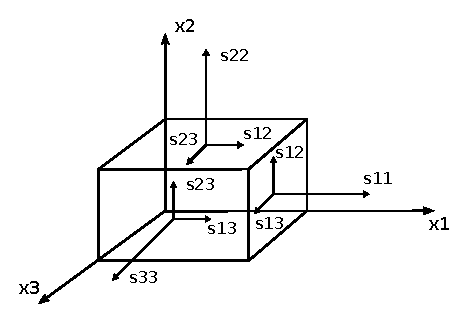
\includegraphics{../images/T1_Ch02-0004}
    \end{center}
    \columnbreak
    \begin{center}
        \psfrag{x1}{$x_1$}
        \psfrag{x2}{$x_2$}
        \psfrag{s11}{$\sigma_{11}$}
        \psfrag{s12}{$\sigma_{12}$}
        \psfrag{s22}{$\sigma_{22}$}
        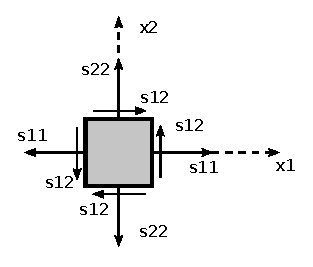
\includegraphics{../images/T1_Ch02-0005}
    \end{center}
\end{multicols}
Les composantes diagonales $\sigma_{11}$, $\sigma_{22}$, $\sigma_{33}$, sont donc des contraintes normales, tandis que les composantes non diagonales $\sigma_{12}$, $\sigma_{13}$, \dots sont des contraintes de cisaillement.
La symétrie du tenseur des contraintes $\sigma_{12} = \sigma_{21}$ exprime l'égalité de la contrainte de cisaillement associée à deux facettes perpendiculaires.
Peur cette raison, cette symétrie est souvent appelée «~principe de réciprocité des cisaillements~».

Dimensionnellement, une «~contrainte~» -- qu'il s'agisse d'une composante du vecteur contrainte ou du tenseur des contraintes -- est homogène à une force par unité de surface, donc à une pression.
L'unité SI, le Pascal ($1 Pa = 1 N/m^2$) étant très petite par rapport aux contraintes habituellement rencontrées, on utilise traditionnellement l'hectobar, le mégapascal et le $daN/mm$ (et chez les anglo-saxons, le p.s.i. \textit{pound per square inch}).
\begin{itemize}
    \item[] 1 daN/mm$^2$ = 1 hectobar = 10 MPa = $10^7$ Pa
\end{itemize}

\subsection{Contraintes principales invariants} \label{ssec:Ch02-1.2}
Le tenseur des contraintes est symétrique; on peut donc le diagonaliser.
Il existe trois directions principales orthogonales associées à trois valeurs propres $\sigma_1$, $\sigma_2$, $\sigma_3$,  appelées «~contraintes principales~».
\begin{equation}
    \sigma_{ij} e_j^{(1)} = \sigma_1 e_i^{(1)},\ \text{ etc.}
    \label{eq:Ch02-008}
\end{equation}
À partir de la décomposition~\eqref{eq:Ch02-003}, on voit qu'une condition nécessaire et suffisante pour qu'une direction soit principale pour $\mathbb{\sigma}$ est que la contrainte exercée sur la facette correspondante soit purement normale (pas de contrainte de cisaillement).
Dans le repère principal, la matrice représentative du tenseur des contraintes est diagonale.
Par abus de langage, on dit que le tenseur des contraintes est diagonal, et on écrit
\begin{equation}
    \mathbb{\sigma} = 
    \begin{bmatrix}
        \sigma_1 & 0 & 0 \\
        0 & \sigma_2 & 0 \\
        0 & 0 & \sigma_3
    \end{bmatrix}
    \label{eq:Ch02-009}
\end{equation}

Les contraintes principales s'obtiennent par résolution de l'équation caractéristique 
\begin{align}
    P_{\mathbb{\sigma}} & = \det
    \begin{bmatrix}
        \sigma_{11}-\lambda & \sigma_{12} & \sigma_{13}\\
        \sigma_{12} & \sigma_{22}-\lambda & \sigma_{23}\\
        \sigma_{13} & \sigma_{22} & \sigma_{33}-\lambda
    \end{bmatrix} \nonumber \\ 
        & = -\lambda^3 + I_1 \lambda^2 - I_2 \lambda + I_3
    \label{eq:Ch02-010}
\end{align}
où $I_1$, $I_2$, $I_3$	sont les invariants de $\mathbb{\sigma}$ définis par (Annexe~\ref{Ann:A})
\begin{equation}
    \left\{
    \begin{aligned}
        I_1 &= \sigma_{ii}= \sigma_1 + \sigma_2 + \sigma_3\\
        I_2 &= \frac{1}{2}\left( \sigma_{ii}\sigma_{jj} - \sigma_{ij}\sigma_{ij} \right) = \sigma_1\sigma_2 + \sigma_2\sigma_3 + \sigma_3\sigma_1\\
        I_3 &= \det \left( \sigma_{ij} \right) = \sigma_1\sigma_2\sigma_3
    \end{aligned}
    \right.
    \label{eq:Ch02-011}
\end{equation}
On 	décompose habituellement le tenseur des contraintes en déviateur et partie sphérique
\begin{equation}
    \sigma_{ij} = \sigma \delta_{ij} + s_{ij}
    \label{eq:Ch02-012}
\end{equation}
où  $\sigma$ est la partie sphérique
\begin{equation}
    \sigma = \frac{1}{3}I_1 = \frac{\sigma_{11} + \sigma_{22} + \sigma_{33}}{3} = \frac{\sigma_1 + \sigma_2 + \sigma_3}{3}
    \label{eq:Ch02-013}
\end{equation}
et où $s_{ij}$ est le déviateur (on appelle déviateur un tenseur de trace nulle)
\begin{equation}
    \left\{
    \begin{aligned}
        & s_{ii} = 0 \qquad s_{ij} = \sigma_{ij} + \frac{1}{3} \sigma_{kk} \delta_{ij}\\
        & s_{12} = \sigma_{12} \qquad s_{11}= \frac{2\sigma_{11} - \sigma_{22} -\sigma_{33}}{3}
    \end{aligned}
    \right.
    \label{eq:Ch02-014}
\end{equation}
Il est clair que le tenseur des contraintes et son déviateur ont mêmes directions principales, les contraintes principales déviatoires $s_1$, $s_2$, $s_3$ sont données par 
\begin{equation}
    s_1 = \frac{2\sigma_1 - \sigma_2 - \sigma_3}{3}
    \label{eq:Ch02-015}
\end{equation}
et les invariants $J_2$, $J_3$ (puisque $J_1 = 0$ par~\eqref{eq:Ch02-014}) du déviateur $s_{ii}$ sont donnés par 
\begin{equation}
    \left\{
    \begin{aligned}
        J_2 &= -\frac{1}{2}s_{ij}s_{ij}\\
        &= s_1 s_2 + s_2 s_3 + s_3 s_1\\
        &= -\frac{1}{2} \left( s_1^2 + s_2^2 + s_3^2 \right)\\
        &= -\frac{1}{6} \left[ \left( \sigma_1 - \sigma_2 \right)^2 + \left( \sigma_2 - \sigma_3 \right)^2 + \left( \sigma_3 -\sigma_1 \right)^2 \right]\\
        J_3 &= \det \left( s_{ij} \right)  = s_1 s_2 s_3
    \end{aligned}
    \right.
    \label{eq:Ch02-016}
\end{equation}
\subsection{États de contraintes particuliers} \label{ssec:Ch02-1.3}
Nous allons envisager divers cas particuliers correspondant à des états de contraintes remarquables. 
\subsubsection{État de tension ou compression hydrostatique}
\begin{equation}
    \mathbb{\sigma} = 
    \begin{bmatrix}
        \sigma & 0 & 0 \\
        0 & \sigma & 0 \\
        0 & 0 & \sigma
    \end{bmatrix}
    \begin{aligned}
        \text{tension si } & \sigma > 0\\
        \text{compression si } & \sigma < 0
    \end{aligned}
    \label{eq:Ch02-017}
\end{equation}
Les trois contraintes principales sont égales, le déviateur est nul, et toutes les directions sont principales.
Sur toute facette s'exerce donc une contrainte purement normale.
\begin{multicols}{2}
    \begin{center}
        \includegraphics{../images/T1_Ch02-0006a}\\
        $\sigma > 0$ (tension)
    \end{center}
    \columnbreak
    \begin{center}
        \includegraphics{../images/T1_Ch02-0006b}\\
        $\sigma < 0$ (compression)
    \end{center}
\end{multicols}
C'est l'état de contraintes qui existe dans les fluides à l'équilibre, d'où la terminologie «~hydrostatique~».
\subsubsection{État  de  contraintes  de  révolution}
\begin{equation}
    \mathbb{\sigma} = 
    \begin{bmatrix}
        \sigma_1 & 0 & 0 \\
        0 & \sigma_2 & 0 \\
        0 & 0 & \sigma_3
    \end{bmatrix}
    \label{eq:Ch02-018}
\end{equation}
Deux des contraintes principales coïncident; les directions principales sont:
\begin{enumerate}
    \item la direction $x_1$, pour $\sigma_1$;
    \item toute direction du plan $\left( x_2, x_3 \right)$, pour $\sigma_2$.
\end{enumerate}
La décomposition en déviateur et partie sphérique devient 
\begin{equation}
    \mathbb{\sigma} = \sigma 
    \begin{bmatrix}
        1 & 0 & 0\\
        0 & 1 & 0\\
        0 & 0 & 1
    \end{bmatrix}
    +
    s
    \begin{bmatrix}
        1 & 0 & 0\\
        0 & -\frac{1}{2} & 0\\
        0 & 0 & -\frac{1}{2}
    \end{bmatrix},\ 
    \sigma = \frac{\sigma_1 + 2\sigma_2}{3} \quad s = \frac{2\left( \sigma_1 - \sigma_2 \right)}{3}
    \label{eq:Ch02-019}
\end{equation}
\begin{multicols}{2}
    \begin{center}
        \psfrag{s1}{$\sigma_1$}
        \psfrag{s2}{$\sigma_2$}
        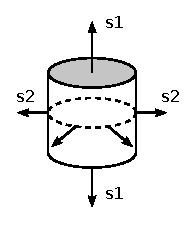
\includegraphics{../images/T1_Ch02-0007a}
    \end{center}
    \columnbreak
    \begin{center}
        \psfrag{s1}{$\sigma_1$}
        \psfrag{s2}{$\sigma_2$}
        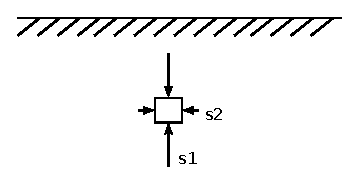
\includegraphics{../images/T1_Ch02-0007b}
    \end{center}
\end{multicols}
C'est l'état de contrainte qui se réalise avec $\sigma_1 <\sigma_2 < 0$ dans le sol en profondeur. 
\subsubsection{État de traction ou compression uniaxiale}
\begin{minipage}[l]{.2\textwidth}
\begin{center}
    \psfrag{s}{$\sigma$}
    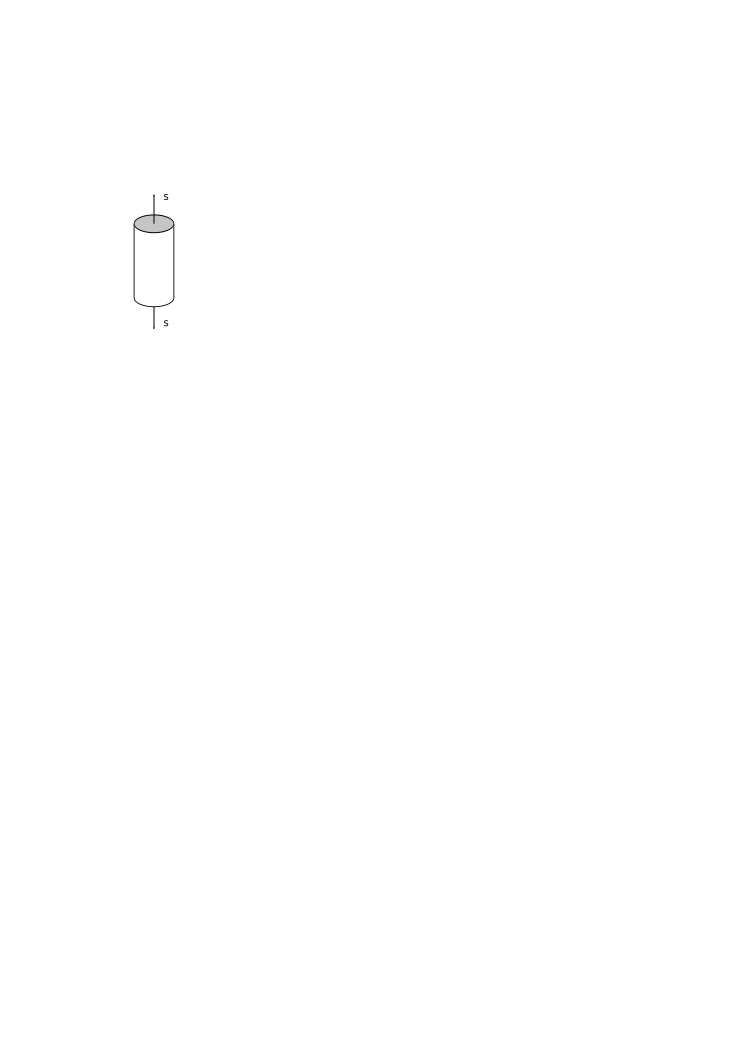
\includegraphics{../images/T1_Ch02-0008}
\end{center}
\end{minipage}
\begin{minipage}[r]{.8\textwidth}
\begin{equation}
    \mathbb{\sigma} = 
    \begin{bmatrix}
        \sigma & 0 & 0 \\
        0 & 0 & 0 \\
        0 & 0 & 0
    \end{bmatrix}
    \begin{aligned}
        \text{traction si } & \sigma > 0\\
        \text{compression si } & \sigma < 0
    \end{aligned}
    \label{eq:Ch02-020}
\end{equation}
C'est un cas particulier du précédent avec $\sigma_2 = 0$ (pas de contrainte latérale). 
C'est l'état de contrainte le plus facile à réaliser expérimentalement: il suffit d'exercer une force longitudinale sur un barreau (essai  de  traction).
\end{minipage}
\subsubsection{État de cisaillement pur}
\begin{equation}
    \mathbb{\sigma} = 
    \begin{bmatrix}
        0 & \tau & 0 \\
        \tau & 0 & 0 \\
        0 & 0 & 0
    \end{bmatrix}
    \label{eq:Ch02-021}
\end{equation}
État de contrainte purement déviatoire.
Les directions principales sont l'axe $x_3$ ($\sigma_3= 0$) et les bissectrices des axes $x_1$, $x_2$ (contraintes principales $+\tau$ et $-\tau$). 
\begin{multicols}{2}
    \begin{center}
        \psfrag{x1}{$x_1$}
        \psfrag{x2}{$x_2$}
        \psfrag{t}{$\tau$}
        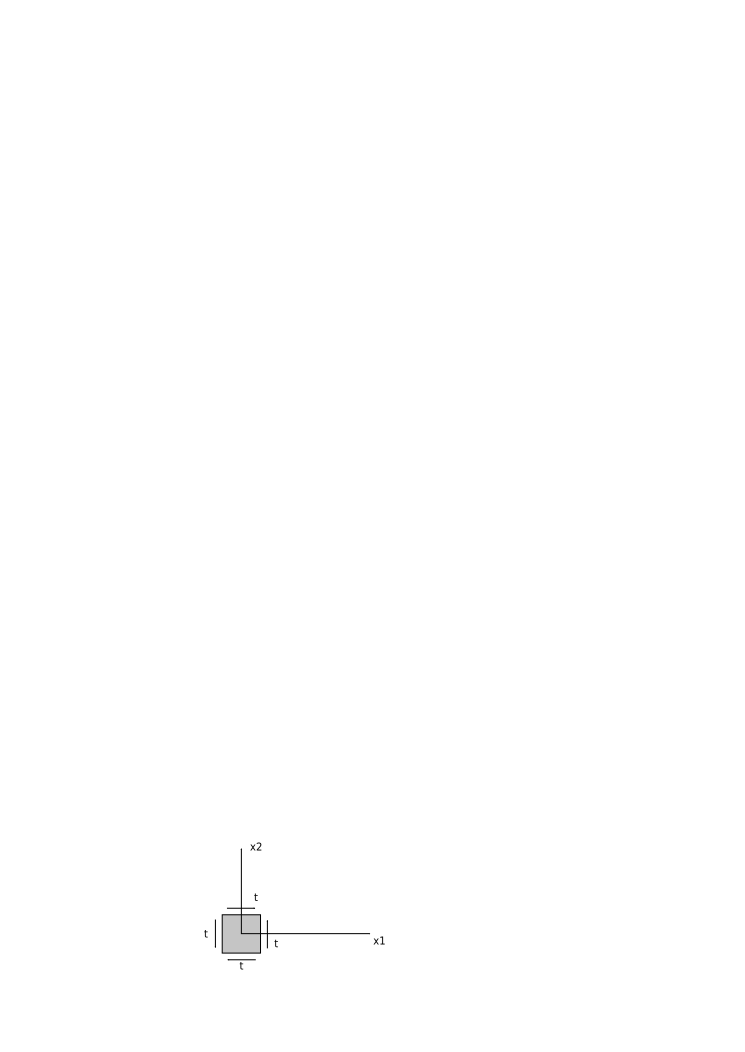
\includegraphics{../images/T1_Ch02-0009a}
    \end{center}
    \begin{center}
        \psfrag{x1}{$x_1$}
        \psfrag{x2}{$x_2$}
        \psfrag{t}{$\tau$}
        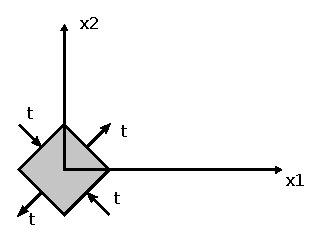
\includegraphics{../images/T1_Ch02-0009b}
    \end{center}
\end{multicols}
\subsubsection{État plan de contraintes}
\begin{equation}
    \mathbb{\sigma} = 
    \begin{bmatrix}
        \sigma_{11} & \sigma_{12} & 0 \\
        \sigma_{12} & \sigma_{22} & 0 \\
        0 & 0 & 0
    \end{bmatrix}
    \text{ ou }
    \begin{bmatrix}
        \sigma_{11} & \sigma_{12} & 0 \\
        \sigma_{12} & \sigma_{22} & 0 \\
        0 & 0 & \sigma_{33}
    \end{bmatrix}
    \label{eq:Ch02-022}
\end{equation}
\begin{minipage}[l]{.3\textwidth}
    \begin{center}
        \psfrag{x1}{$x_1$}
        \psfrag{x2}{$x_2$}
        \psfrag{s11}{$\sigma_{11}$}
        \psfrag{s22}{$\sigma_{22}$}
        \psfrag{s12}{$\sigma_{12}$}
        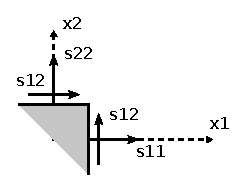
\includegraphics{../images/T1_Ch02-0010}
    \end{center}
\end{minipage}
\begin{minipage}[r]{.7\textwidth}
Les directions principales sont la direction $x_3$ et deux directions perpendiculaires du plan $x_1$, $x_2$.
Lorsque $\vec{n}$ varie dans le plan $x_1$, $x_2$, le vecteur contrainte reste dans le plan, et on peut se limiter au plan $x_1$, $x_2$.
Nous ferons l'étude complète au paragraphe~\ref{ssec:Ch02-3.2}.
\end{minipage}

\section{Représentations géométriques des contraintes} \label{sec:Ch2-2}
L'état de contraintes en un point donné est caractérisé par la valeur en ce point du tenseur des contraintes, c'est à dire par 6 nombres.
Pour visualiser cette entité, on a introduit diverses représentations géométriques.
\subsection{Quadriques des contraintes} \label{ssec:Ch02-2.1}
\subsubsection{Ellipsolde de Lamé}
C'est le lieu de l'extrémité du vecteur contrainte $\vec{T}$ lorsque $\vec{n}$ varie.
Si nous nous plaçons en repère principal, l'équation~\eqref{eq:Ch02-005} donne 
\begin{equation*}
    T_1 = \sigma_1 n_1 \qquad T_2 = \sigma_2 n_2 \qquad T_3 = \sigma_3 n_3
\end{equation*}
et, puisque le vecteur $vec{n}$ est unitaire 
\begin{equation}
    \frac{T_1^2}{\sigma_1^2} + \frac{T_2^2}{\sigma_2^2} + \frac{T_3^2}{\sigma_3^2} = 1
    \label{eq:Ch02-023}
\end{equation}
Le lieu de l'extrémité ($T_1$, $T_2$, $T_3$) est un ellipsoïde d'axes principaux sont les directions principales du tenseur des contraintes et de demi-axe les valeurs absolues des contraintes principales -- c'est l'el1ipsoïde de Lamé.
Mais cet ellipsoïde ne permet pas de visualiser le vecteur contrainte associé à une facette donnée.
\subsubsection{Quadrique directrice des contraintes normales}
Nous considérons la (ou les) quadrique(s) réelle(s) d'équation 
\begin{equation}
    \Phi(x) = \sigma_{ij} x_i x_j = \pm 1
    \label{eq:Ch02-024}
\end{equation}
C'est une (ou deux) quadrique(s) d'axes principaux les directions principales du tenseur des contraintes et de demi-axes ($1/\sqrt{|\sigma_1|}$, \ldots).
On les appelle quadriques directrices des contraintes, car elles permettent de construire le vecteur contrainte associé à une direction $\vec{n}$ quelconque par la construction suivante. 

\noindent\underline{Construction:} On mène de l'origine la demi-droite de direction $\vec{n}$, qui coupe la quadrique en un point $M$.  
\begin{itemize}
    \item la contrainte normale  est donnée  à  partir de  la longueur $OM=\rho$ par
        \begin{equation}
            \rho^2 |T_n| = 1
            \label{eq:Ch02-025}
        \end{equation}
    \item la direction du vecteur contrainte est donnée par la normale $\vec{N}$ à la quadrique en $M$. 
\end{itemize}
\begin{multicols}{2}
    \begin{center}
        \psfrag{x1}{$x_1$}
        \psfrag{x2}{$x_2$}
        \psfrag{x3}{$x_3$}
        \psfrag{n}{$\vec{n}$}
        \psfrag{N}{$\vec{N}$}
        \psfrag{M}{M}
        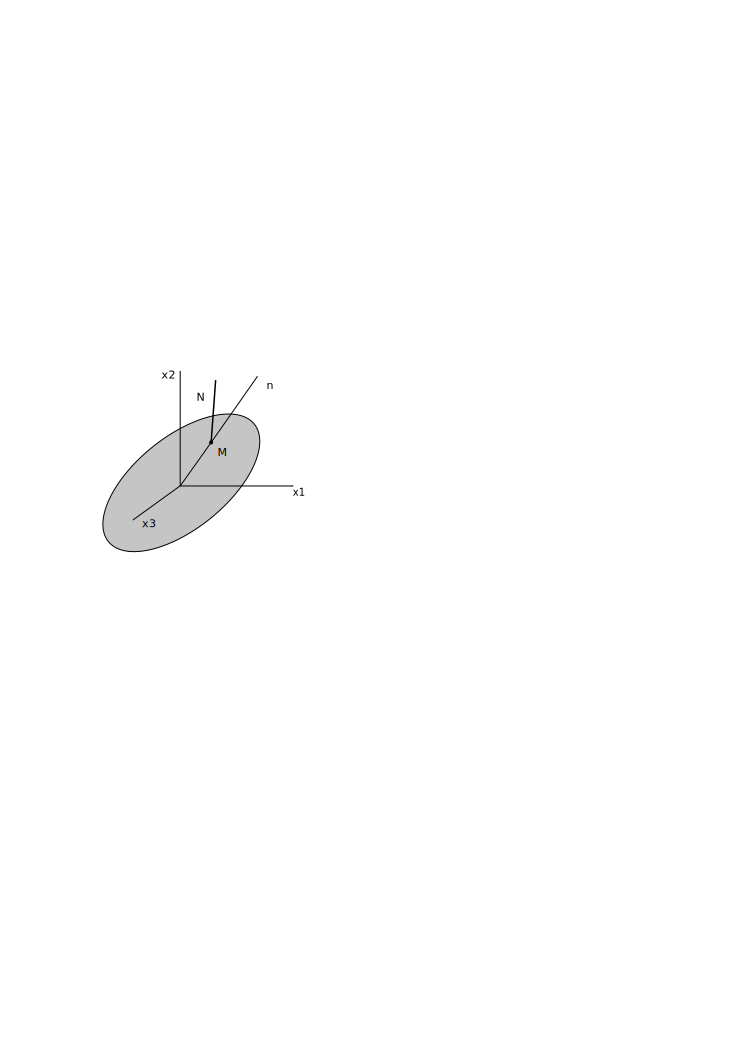
\includegraphics{../images/T1_Ch02-0011}
    \end{center}
    \columnbreak
    \begin{proof}
        On a $\vec{OM} = p \vec{n},\ x_i = p n_i$.
    En reportant dans~\eqref{eq:Ch02-024}, il vient
    \begin{displaymath}
        \rho^2 \sigma_{ij} n_i n_j = \pm 1
    \end{displaymath}
    qui donne~\eqref{eq:Ch02-025}, en remarquant que
    \begin{displaymath}
        T_n = \vec{T} \cdot \vec{n} = \sigma_{ij} n_i n_j
    \end{displaymath}
    La direction de la normale $\vec{N}$ à la quadrique donnée par le gradient de la fonction $\Phi$  est  
    \begin{displaymath}
        N_i = \lambda \frac{\partial \Phi}{\partial x_i} = 2\lambda \sigma_{ij} x_j = 2 \lambda \rho \sigma_{ij} n_j = 2 \lambda \rho T_i
    \end{displaymath}
    et $\vec{N}$ est proportionnel à $\vec{T}$.
    \end{proof}
\end{multicols}
Si toutes les contraintes principales sont de même signe, la forme quadratique 
\begin{equation}
    T_n = \sigma_{ij} n_i n_j
    \label{eq:Ch02-026}
\end{equation}
est définie positive ou négative, et \eqref{eq:Ch02-024} définit un ellipsoïde.
Si les contraintes principales sont certaines positives et d'autres négatives, alors $T_n$ peut être positif ou négatif, et \eqref{eq:Ch02-024} définit deux hyperboloïdes limités par le cône asymptote $T_n = 0$.
Enfin, si une contrainte principale est nulle, \eqref{eq:Ch02-024} définit un cylindre elliptique ou hyperbolique, suivant le signe des deux autres valeurs propres. 
\subsection{Espace des contraintes principales} \label{ssec:Ch02-2.2}
Le tenseur des contraintes (ou plus généralement tout tenseur symétrique) peut être caractérisé par les trois contraintes principales et l'orientation du repère principal.
Dans de nombreux cas, l'orientation du repère principal ne joue pas un rôle essentiel, et on pourra caractériser le tenseur des contraintes par les trois contraintes principales $\sigma_1$, $\sigma_2$, $\sigma_3$.
On peut donc représenter un tenseur des contraintes par un point d'un espace à trois dimensions $O\sigma_1\sigma_2\sigma_3$: au tenseur $\mathbb{\sigma}$ on associe le point $\Sigma$ ayant comme coordonnées les contraintes principales $\sigma_1$, $\sigma_2$, $\sigma_3$ de $\mathbb{\sigma}$ (le repère $O\sigma_1\sigma_2\sigma_3$ étant postulé orthonormé).

\begin{wrapfigure}[15]{l}{.55\textwidth}
    \begin{center}
        \psfrag{P}{$\Pi$}
        \psfrag{S}{$S$}
        \psfrag{O}{$O$}
        \psfrag{s1}{$\sigma_1$}
        \psfrag{s2}{$\sigma_2$}
        \psfrag{s3}{$\sigma_3$}
        \psfrag{E}{$\Sigma$}
        \psfrag{E'}{$\Sigma'$}
        \psfrag{D}{$\Delta$}
        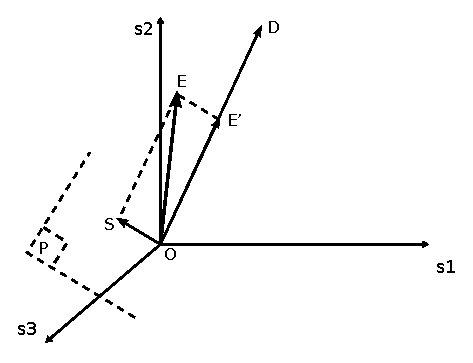
\includegraphics{../images/T1_Ch02-0012}
    \end{center}
\end{wrapfigure}
Cette représentation, très utile, exige néanmoins certaines précautions: on représente géométriquement l'espace des contraintes principales par un espace vectoriel mais ce n'est pas un espace vectoriel.
En particulier, les changements d'axes sont dépourvus de sens.
En particulier également, la somme de deux tenseurs $\sigma_{ij}^{(1)} + \sigma_{ij}^{(2)}$ ne correspond pas à la somme vectorielle (sauf dans le cas où les tenseurs $\sigma_{ij}^{(1)}$ et $\sigma_{ij}^{(2)}$ ont mêmes directions principales).
Enfin, un tenseur des contraintes est représenté, en toute rigueur, non pas par un point, mais par 6 points, car la numérotation des valeurs propres $\sigma_1$, $\sigma_2$, $\sigma_3$ est arbitraire. 

Dans cet espace, les tenseurs sphériques sont représentés par les points de l'«~axe hydrostatique $\Delta$~» (cosinus directeurs: $1/\sqrt{3},\ 1/\sqrt{3},\ 1/\sqrt{3}$).
Les déviateurs sont représentés par les points du plan déviatoire $\Pi$ , perpendiculaire en O à l'axe hydrostatique $\Delta$
\begin{equation}
    \sigma_1 + \sigma_2 + \sigma_3 = 0
    \label{eq:Ch02-027}
\end{equation}
La décomposition~\eqref{eq:Ch02-012} d'un tenseur en partie sphérique et déviateur correspond à la projection orthogonale sur $\Delta$ et $\Pi$.
En particulier, la projection sur $\Delta$ est caractérisée par la trace de $\mathbb{\sigma}$.
Dans le plan déviatoire $\Pi$ on trace 
\begin{center}
    \psfrag{Plan P}{Plan $\Pi$}
    \psfrag{S}{$S$}
    \psfrag{s1}{$\sigma_1$}
    \psfrag{s2}{$\sigma_2$}
    \psfrag{s3}{$\sigma_3$}
    \psfrag{r}{$r$}
    \psfrag{t}{$\theta$}
    \psfrag{h1}{$\vec{h}_1$}
    \psfrag{h2}{$\vec{h}_2$}
    \psfrag{h3}{$\vec{h}_3$}
    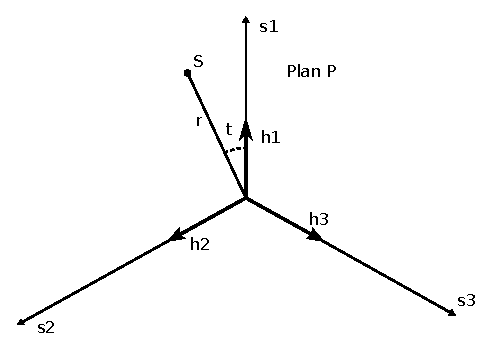
\includegraphics{../images/T1_Ch02-0013}
\end{center}
la projection des axes $O\sigma_1$, $O\sigma_2$, $O\sigma_3$, qui font entre eux un angle de $2\pi/3$ et un tenseur $\mathbb{\sigma}$ sera représenté par le point $S$
\begin{equation}
    \vec{OS} = \sigma_1 \vec{h}_1 + \sigma_2 \vec{h}_2 + \sigma_3 \vec{h}_3
    \label{eq:Ch02-028}
\end{equation}
$\vec{h}_1$, $\vec{h}_2$, $\vec{h}_3$ étant les trois vecteurs unitaires portés par les axes $O\sigma_1$, $O\sigma_2$, $O\sigma_3$ -- ou plutôt par leurs projections, mais nous les notons encore $O\sigma_1$, $O\sigma_2$, $O\sigma_2$, $O\sigma_3$.
En particulier, on vérifie bien que le point $S$ ainsi construit caractérise le déviateur, puisque, si l'on rajoute à $\mathbb{\sigma}$ un tenseur sphérique arbitraire, le point $S$ ne change pas, car $\vec{h}_1 + \vec{h}_2 + \vec{h}_3 = 0$.

On peut alors montrer que la position du point $S$ est complètement caractérisée par les deux invariants $J_2$ et $J_3$ introduits par~\eqref{eq:Ch02-016}.
Plus précisément, un calcul direct montre que les coordonnées polaires $\left( r,\ \theta \right)$ de $S$ sont données par 
\begin{equation}
    r = \sqrt{-3J_2},\ \cos 3 \theta = \frac{3\sqrt{3}}{2}\frac{J_3}{J_2^{3/2}}
    \label{eq:Ch02-029}
\end{equation}
Le second invariant $J_2$ détermine la distance $OS$, c'est à dire «~l'intensité~» du déviateur, tandis que le troisième invariant $J_3$ détermine son orientation. 
Plus précisément, on constate que l'on a 
\begin{align}
    3\theta &= \pm \arccos \left( \frac{3\sqrt{3}}{2} \frac{J_3}{J_2^{3/2}} \right) + 2 k \pi\nonumber\\
    \theta &= \pm \frac{1}{3}\arccos \left( \frac{3\sqrt{3}}{2} \frac{J_3}{J_2^{3/2}} \right) + \frac{2 k \pi}{3}
\end{align}
\begin{wrapfigure}[9]{r}{.4\textwidth}
    \begin{center}
        \psfrag{s1}{$\sigma_1$}
        \psfrag{s2}{$\sigma_2$}
        \psfrag{s3}{$\sigma_3$}
        \psfrag{S1}{$S_1$}
        \psfrag{S2}{$S_2$}
        \psfrag{S3}{$S_3$}
        \psfrag{S4}{$S_4$}
        \psfrag{S5}{$S_5$}
        \psfrag{S6}{$S_6$}
        \psfrag{O}{$O$}
        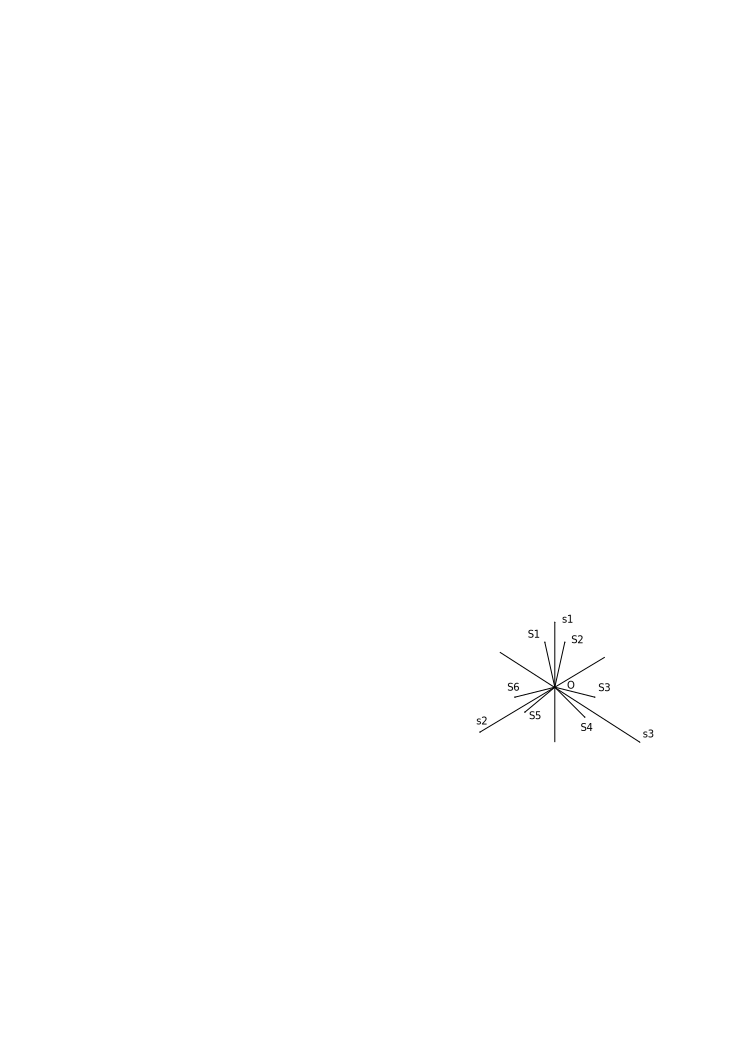
\includegraphics{../images/T1_Ch02-0014}
    \end{center}
\end{wrapfigure}
ce qui donne les 6 points $S$ correspondant aux 6 numérotations possibles des trois valeurs propres. 
Si l'on impose par exemple $\sigma_1 > \sigma_2 > \sigma_3$ alors on se restreint au quartier $O\sigma_1\sigma_3^{\prime}$ et le point $S$ est complètement défini. 

Finalement, on constate que la position du point $\Sigma$ dans l'espace des contraintes principales est complètement caractérisée par $I_1$, $J_2$, $J_3$: $I_1$ fixe la projection sur $\Delta$, $J_2$ la distance à $\Delta$ et $J_3$ l'orientation de la projection de $O\Sigma$ sur $\Pi$.

\section{Représentation de Mohr} \label{sec:Ch02-3}
\subsection{Tricercle de Mohr} \label{ssec:Ch02-3.1}
La représentation de Mohr est une représentation dans le plan des contraintes normales et tangentielles. 
On porte en abscisse la contrainte normale (algébrique) et en ordonnée le module de la contrainte tangentielle.
\begin{center}
    \psfrag{s1}{$\sigma_1$}
    \psfrag{s2}{$\sigma_2$}
    \psfrag{s3}{$\sigma_3$}
    \psfrag{M1}{$M_1$}
    \psfrag{M2}{$M_2$}
    \psfrag{M3}{$M_3$}
    \psfrag{M}{$M$}
    \psfrag{O}{$O$}
    \psfrag{Tt}{$|\vec{T}_t|$}
    \psfrag{Tn}{$T_n$}
    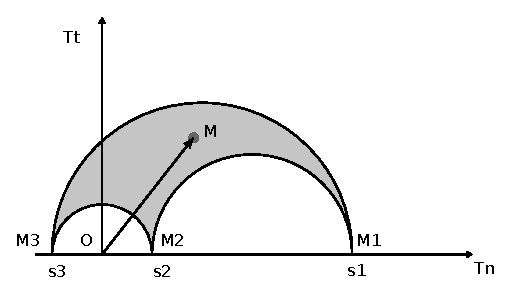
\includegraphics{../images/T1_Ch02-0015}
\end{center}
On obtient ainsi un point $M$ pour chaque facette, et on cherche le lieu de ces points lorsque l'on fait varier la facette.
Pour faire les calculs, on se place en repère principal du tenseur des contraintes et on suppose les valeurs propres rangées par ordre décroissant, $\sigma_3 < \sigma_2 < \sigma_1$.
Les points $M_1$, $M_2$ et $M_3$ correspondant aux facettes normales aux directions principales sont sur l'axe des contraintes normales.
Pour une facette quelconque, on a
\begin{displaymath}
    T_1 = \sigma_1 n_1 \quad T_2 = \sigma_2 n_2 \quad T_3 = \sigma_3 n_3
\end{displaymath}
qui permet de calculer $T_n = T_i n_i$ et $|T|^2 = T_n^2 + T_t^2$
\begin{equation}
    T_n = \sigma_1 n_1^2 + \sigma_2 n_2^2 + \sigma_3 n_3^2
    \label{eq:Ch02-031}
\end{equation}
\begin{equation}
    T_n^2 + T_t^2 = \sigma_1^2 n_1^2 + \sigma_2^2 n_2^2 + \sigma_3^2 n_3^2
    \label{eq:Ch02-032}
\end{equation}
Etant donnée une valeur de $T_n$ et de $T_t$, peut-on trouver une facette qui leur corresponde ?
Pour cela, il faut calculer $n_1$, $n_2$, $n_3$ à partir du système formé par \eqref{eq:Ch02-031}, \eqref{eq:Ch02-032} et la relation 
\begin{equation}
    1 = n_1^2 + n_2^2 + n_3^2
    \label{eq:Ch02-033}
\end{equation}
exprimant le fait que le vecteur $\vec{n}$ est unitaire.
On a donc un système linéaire en $n_1^2$, $n_2^2$, $n_3^2$, dont la solution est 
\begin{equation}
    n_1^2 = \frac{T_t^2 + \left( T_n - \sigma_2 \right)\left( T_n - \sigma_3 \right)}{\left( \sigma_1 - \sigma_2 \right)\left( \sigma_1 - \sigma_3 \right)}
    \label{eq:Ch02-034}
\end{equation}
et $n_2^2$, $n_3^2$, par permutation circulaire.
Géométriquement, on retrouve au dénominateur le produit scalaire $\vec{M_1M_2}\cdot\vec{M_1M_3}$ et au numérateur le produit scalaire $\vec{MM_2}\cdot \vec{MM_3}$.
On a donc 
\begin{equation}
    n_1^2 = \frac{\vec{MM_2} \cdot \vec{MM_3}}{\vec{M_1M_2} \cdot \vec{M_1M_3}},\quad n_2^2 = \frac{\vec{MM_1} \cdot \vec{MM_3}}{\vec{M_2M_1} \cdot \vec{M_2M_3}},\quad n_3^2 = \frac{\vec{MM_1} \cdot \vec{MM_2}}{\vec{M_3M_1} \cdot \vec{M_3M_2}}
    \label{eq:Ch02-035}
\end{equation}
Pour que cette solution soit satisfaisante, il faut vérifier que $n_1^2$, $n_2^2$ et $n_3^2$ sont positifs 
\begin{equation}
    n_1^2 \geq 0, n_2^2 \geq 0, n_3^2 \geq 0, 
    \label{eq:Ch02-036}
\end{equation}
Or, puisque $\sigma_3 < \sigma_2 < \sigma_1$, il est clair que
\begin{equation}
    \vec{M_1M_2} \cdot \vec{M_1M_3} \geq 0, \quad \vec{M_2M_1} \cdot \vec{M_2M_3} \leq 0, \quad \vec{M_3M_1} \cdot \vec{M_3M_2} \geq 0
    \label{eq:Ch02-037}
\end{equation}
Les conditions~\eqref{eq:Ch02-036} exigent donc 
\begin{equation}
    \vec{MM_2} \cdot \vec{MM_3} \geq 0, \quad \vec{MM_1} \cdot \vec{MM_3} \leq 0, \quad \vec{MM_1} \cdot \vec{MM_2} \geq 0
    \label{eq:Ch02-038}
\end{equation}
c'est à dire que les angles $\left( \vec{MM_2},\vec{MM_3} \right)$ et  $\left( \vec{MM_1},\vec{MM_2} \right)$ soient aigus et l'angle $\left( \vec{MM_1}, \vec{MM_3} \right)$ soit obtus, c'est à dire encore que le point $M$ soit à l'extérieur des deux demi-cercles de diamètres $M_1M_2$ et $M_2M_3$, et à l'intérieur du demi-cercle de diamètre $M_1M_3$.
Ainsi, quand $\vec{n}$ varie, le point $M$ reste dans la surface hachurée appelée -- tricercle de Mohr -- et qui devient un demi cercle si deux valeurs propres coïncident, et un point pour un tenseur sphérique.

On constate d'autre part que $M$ décrit le demi cercle de diamètre $M_1M_3$ lorsque $\vec{n}$ varie dans le plan $\vec{e}_1, \vec{e}_3$ (car \eqref{eq:Ch02-035} montre que $n_2 = 0$  si et seulement si $\vec{MM_1}$ est orthogonal à $\vec{MM_3}$).
On voit également que le maximum de la contrainte de cisaillement (lorsque l'on fait varier la facette) est égale au rayon du plus grand cercle, c'est à dire à la demi différence des contraintes principales extrêmes
\begin{equation}
    |T_t|_{max} = \frac{\sigma_1 - \sigma_3}{2} = \frac{1}{2} \max_{i,j} |\sigma_i - \sigma_j|
    \label{eq:Ch02-039}
\end{equation}
On montrera au paragraphe~\ref{ssec:Ch02-3.2} que ce maximum est atteint lorsque $\vec{n}$ est bissectrice des directions principales.  

\subsection{Cercle de Mohr -- Pole} \label{ssec:Ch02-3.2}
Nous considérons maintenant un état plan de contraintes~\eqref{eq:Ch02-022}, et nous faisons varier $\vec{n}$, dans le plan $\left( x_1,x_2 \right)$.
On peut alors orienter la direction tangentielle à la facette en introduisant un vecteur unitaire $\vec{t}$ à $+\pi/2$ de $\vec{n}$.
La contrainte tangentielle $T_t$ devient donc une quantité algébrique, et la représentation dans le plan de Mohr permet de déterminer l'orientation du vecteur contrainte. 
\begin{multicols}{2}
    \begin{center}
        \psfrag{x1}{$x_1$}
        \psfrag{x2}{$x_2$}
        \psfrag{x1'}{$x_1'$}
        \psfrag{x2'}{$x_2'$}
        \psfrag{t}{$\theta$}
        \psfrag{Tt}{$T_t$}
        \psfrag{Tn}{$T_n$}
        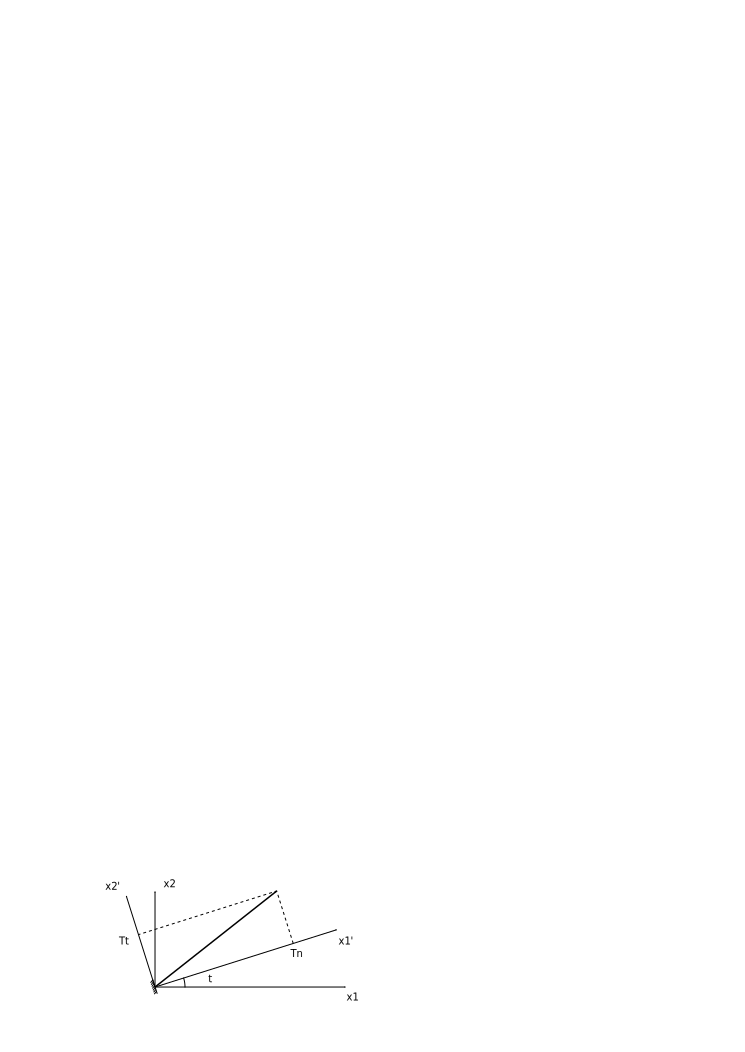
\includegraphics{../images/T1_Ch02-0016a}
    \end{center}
    \columnbreak
    \begin{center}
        \psfrag{Tn}{$T_n$}
        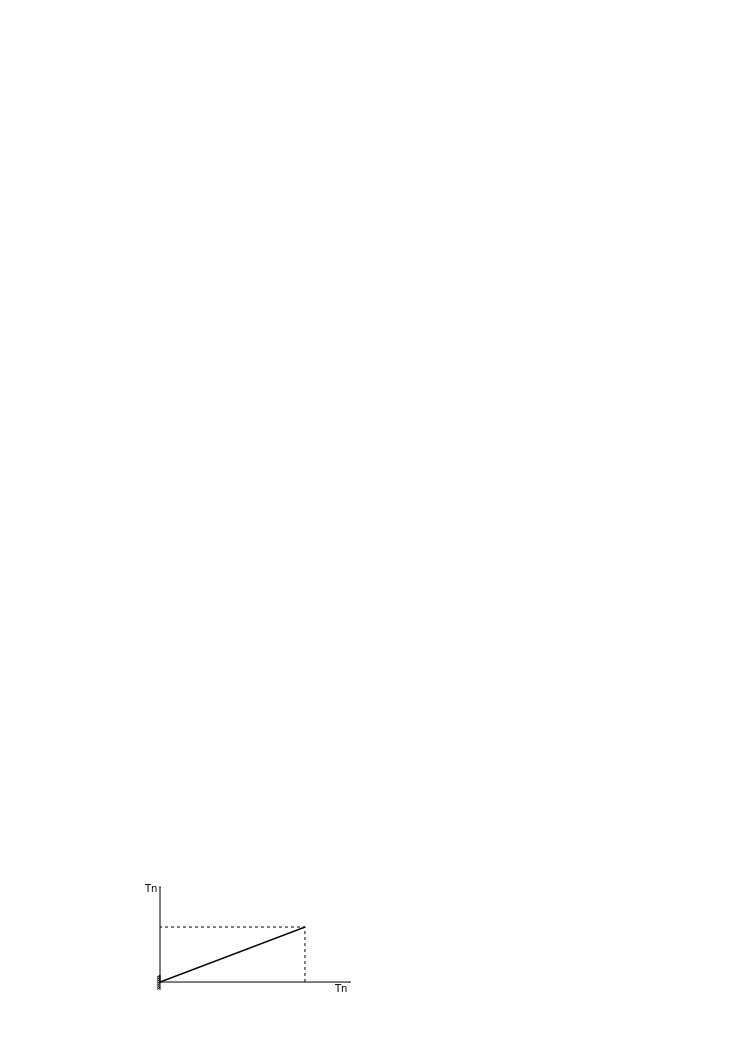
\includegraphics{../images/T1_Ch02-0016b}
    \end{center}
\end{multicols}
Pour calculer $T_n$ et $T_t$ on écrit
\begin{displaymath}
    \vec{n} = 
    \begin{bmatrix}
        \cos \theta\\
        \sin \theta
    \end{bmatrix}
    \quad
    \vec{t} = 
    \begin{bmatrix}
        -\sin \theta
        \cos \theta
    \end{bmatrix}
\end{displaymath}
on calcule le vecteur contrainte
\begin{equation}
    \left\{
    \begin{array}{lll}
        T_1 & = \sigma_{11} \cos \theta & + \sigma_{12} \sin \theta\\
        T_2 & = \sigma_{12} \cos \theta & + \sigma_{22} \sin \theta
    \end{array}
    \right.
    \label{eq:Ch02-040}
\end{equation}
et ensuite et en projetant $T_n$ et $T_t$ sur $\vec{n}$ et $\vec{t}$
\begin{equation}
    \left\{
    \begin{aligned}
        T_n &= \sigma_{11} \cos^2 \theta + 2 \sigma_{12} \cos \theta \sin \theta + \sigma_{22} \sin^2 \theta\\
            &= \frac{\sigma_{11} + \sigma_{22}}{2} + \frac{\sigma_{11} - \sigma_{22}}{2} \cos 2 \theta + \sigma_{12} \sin 2 \theta\\
        T_t &= \left(\sigma_{22}-\sigma_{11}\right) \cos \theta \sin \theta + \sigma_{12} \left( \cos^2\theta -\sin^2 \theta \right)\\
            &= -\frac{\left(\sigma_{11}-\sigma_{22}\right)}{2} + \sigma_{12} \cos 2 \theta
    \end{aligned}
    \right.
    \label{eq:Ch02-041}
\end{equation}
Les directions principales s'obtiennent en annulant la contrainte tangentielle $T_t = 0$:
\begin{equation}
    \tan 2 \theta_0 = \frac{2\sigma_{12}}{\sigma_{11} - \sigma_{22}}
    \label{eq:Ch02-042}
\end{equation}
ce qui définit $\theta_0$ à $k\pi/2$ près.
Nous choisissons $\theta_0$ en posant 
\begin{equation}
    \left\{
    \begin{aligned}
        \sigma_{12} &= \sqrt{\left( \frac{\sigma_{11} - \sigma_{12}}{2} \right)^2 + \sigma_{12}^2} \sin 2 \theta_0 \\
        \frac{\sigma_{11} - \sigma_{22}}{2} &= \sqrt{\left( \frac{\sigma_{11} - \sigma_{12}}{2} \right)^2 + \sigma_{12^2}} \cos 2 \theta_0
    \end{aligned}
    \right.
    \label{eq:Ch02-043}
\end{equation}
En reportant dans \eqref{eq:Ch02-043}, on obtient alors 
\begin{equation}
    \begin{aligned}
        T_n &= \frac{\sigma_{11} + \sigma_{22}}{2} + \sqrt{\left( \frac{\sigma_{11} - \sigma_{22}}{2} \right)^2 + \sigma_{12}^2} \cos 2 \left( \theta_0 - \theta \right)\\
        T_t &= \sqrt{\left( \frac{\sigma_{11} - \sigma_{22}}{2} \right)^2 + \sigma_{12}^2} \sin 2 \left( \theta_0 - \theta \right)
    \end{aligned}
    \label{eq:Ch02-044}
\end{equation}
Lorsque $\theta$ varie, le point $M$, représentant le vecteur contrainte dans le plan $T_n$, $T_t$, décrit un cercle de centre $\Omega$ et rayon $R$
\begin{equation}
    \Omega = \left( \frac{\sigma_{11}+\sigma_{22}}{2}, 0 \right), \ R = \sqrt{\left( \frac{\sigma_{11} - \sigma_{22}}{2} \right)^2 + \sigma_{12}^2}
    \label{eq:Ch02-045}
\end{equation}
\begin{center}
    \psfrag{Tt}{$T_t$}
    \psfrag{Tn}{$T_n$}
    \psfrag{A1}{$A_1$}
    \psfrag{A2}{$A_2$}
    \psfrag{B1}{$B_1$}
    \psfrag{B2}{$B_2$}
    \psfrag{M1}{$M_1$}
    \psfrag{M2}{$M_2$}
    \psfrag{2t}{$2\theta$}
    \psfrag{2t0}{$2\theta_0$}
    \psfrag{s11}{$\sigma_{11}$}
    \psfrag{s12}{$\sigma_{12}$}
    \psfrag{-s12}{$-\sigma_{12}$}
    \psfrag{s22}{$\sigma_{22}$}
    \psfrag{x1}{$x_1$}
    \psfrag{x2}{$x_2$}
    \psfrag{O}{$O$}
    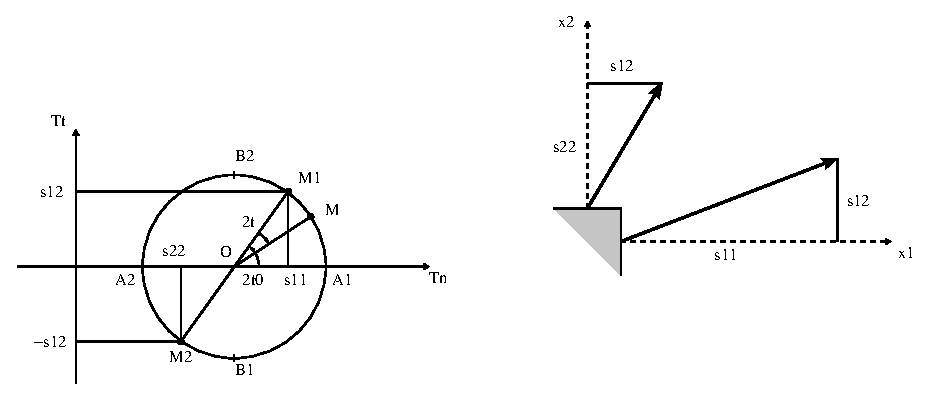
\includegraphics{../images/T1_Ch02-0017}
\end{center}
Les points  et $M_1\ \left( \sigma_{11},\ \sigma_{12} \right)$ et $M_2\ \left( \sigma_{22},\ -\sigma_{12} \right)$ correspondent à $\vec{n} = \vec{e}_1$ et $\vec{n}=\vec{e}_2$ respectivement. 
Pour obtenir le point $M$ correspondant à une normale $\vec{n}$ formant un angle $\theta$ avec $\vec{e}_1$, il faut tourner par rapport à $\Omega M_1$ d' un angle $2\theta$ dans le sens rétrograde.
Les points $A_1$ et $A_2$ correspondent aux directions principales, $\theta = \theta_0 + k\pi/2$ et les contraintes principales sont données par 
\begin{equation}
    \sigma_{1\text{ ou }2} = \frac{\sigma_{11} + \sigma_{22}}{2} \pm \sqrt{\left( \frac{\sigma_{11} - \sigma_{22}}{2} \right)^2 +\sigma_{12}^2}
    \label{eq:Ch02-046}
\end{equation}
Les points $B_1$ et $B_2$ correspondent aux directions de cisaillement maximal et sont donnés par $\theta = \theta_0 + \pi/4 + k\pi/2$, ce sont donc les bissectrices des directions principales, comme annoncé à la fin du paragraphe~\ref{ssec:Ch02-3.1}. 

Le point $M_1$ est appelé pôle du cercle de Mohr, et il permet une construction graphique du vecteur contrainte associé à une facette quelconque.
\begin{center}
    \psfrag{Tt}{$T_t$}
    \psfrag{Tn}{$T_n$}
    \psfrag{A1}{$A_1$}
    \psfrag{A2}{$A_2$}
    \psfrag{B1}{$B_1$}
    \psfrag{B2}{$B_2$}
    \psfrag{M}{$M$}
    \psfrag{M'}{$M'$}
    \psfrag{M1}{$M_1$}
    \psfrag{M1'}{$M_1'$}
    \psfrag{M2}{$M_2$}
    \psfrag{t}{$\theta$}
    \psfrag{2t}{$2\theta$}
    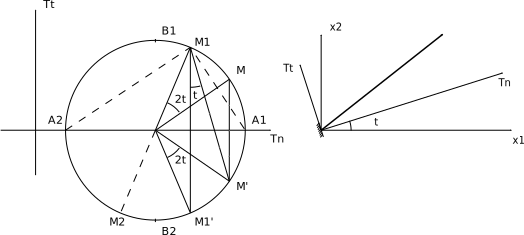
\includegraphics{../images/T1_Ch02-0018}
\end{center}
Pour obtenir le point $M$, c'est à dire le vecteur contrainte s'exerçant sur une facette inclinée de $\theta$ par rapport à la verticale, on utilise la construction suivante.
\begin{enumerate}
    \item On trace $M_1 M^{\prime}$ parallèle à la facette considérée, qui coupe le cercle de Mohr en $M^{\prime}$.
    \item $M$ est le symétrique de $M^{\prime}$ par rapport à l'axe des $T_n$.
\end{enumerate}
On en tire en particulier les directions principales $M_1 A_1$ et $M_1 A_2$ ainsi que les directions de contrainte tangentielle maximum $M_1 B_1$ et $M_1 B_2$. 


\chapter{Étude des déformations} \label{chap:Ch03}
\section{Grandes déformations} \label{sec:Ch03-1}
\subsection{Description de la déformation} \label{ssec:Ch03-1.1}
% Generated with LaTeXDraw 2.0.5
% Sun Nov 08 14:17:03 EST 2009
\scalebox{1} % Change this value to rescale the drawing.
{
\begin{pspicture}(0,-4)(14.744687,3.2425)
\psdots[fillstyle=solid,dotstyle=o](12.864688,1.5225)
\rput(4.8,0.7275){$\vec{\ud a}$}
\psdots[fillstyle=solid,dotstyle=o](5.0446873,0.3225)
\psdots[fillstyle=solid,dotstyle=o](5.4446874,1.3225)
\psline{->}(2.4646876,-1.2775)(2.4646876,2.3225)
\psline{->}(2.4646876,-1.2575)(6.8646874,-1.2575)
\psline{->}(2.4646876,-1.2575)(1.1046875,-2.8575)
\psbezier[linewidth=0.04](4.4646873,1.9225)(3.5646906,1.4866039)(3.1716466,0.11810785)(3.5246875,-0.8175)(3.8777285,-1.7531079)(4.424077,-2.4369879)(5.3646874,-2.0975)(6.305298,-1.7580122)(7.0475364,0.19629975)(6.6246877,1.1025)(6.2018385,2.0087004)(5.3646846,2.3583963)(4.4646873,1.9225)
\psline{->}(5.0646877,0.3225)(5.4446874,1.3425)
\psbezier[linewidth=0.02](5.0846877,0.3425)(6.0046873,1.2352536)(9.8046875,1.8425)(11.644688,0.9425)
\psdots[fillstyle=solid,dotstyle=o](11.644688,0.9225)
\psline{->}(11.684688,0.9425)(12.884687,1.5225)
\rput(6.909219,-1.5325){$x_1$}
\rput(3.1492188,2.4075){$x_2$}
\rput(1.8292187,-3.0325){$x_3$}
\rput(0.978125,0.1875){Repère fixe}
\rput(4.8392186,-0.0325){$M$}
\rput(4.8992186,1.5475){$M'$}
\rput(11.459219,0.5475){$M_t$}
\rput(13.119219,1.8475){$M_t'$}
\psbezier[linewidth=0.04](9.704687,-1.4775)(8.544687,0.0425)(11.924687,3.2225)(13.324688,2.4025)(14.724688,1.5825)(13.884687,1.1825)(12.964687,0.8225)(12.044687,0.4625)(10.864688,-2.9975)(9.704687,-1.4775)
\rput(4.845625,-2.6325){Configuration de référence}
\rput(10.955625,-2.6325){Configuration actuelle}
\rput(12.357187,-1.5125){instant $t$}
\psbezier[linewidth=0.02](5.4846873,1.3225)(7.2846875,2.4825)(10.884687,2.6425)(12.844687,1.5225)
\end{pspicture} 
}

Pour repérer la position d'une particule d'un milieu continu, il faut introduire un repère d'espace supposé fixe au cours du temps: un référentiel.
En général on choisit un référentiel galiléen, sinon il faut rajouter les forces d'inertie dans les forces de volume $f_i$.
Le mouvement est décrit par la fonction
\begin{equation}
    x_i = x_i \left( a_1, a_2, a_3, t \right) \quad i = 1, 2, 3
    \label{eq:Ch03-001}
\end{equation}
donnant la position à l'instant $t$, $M_t$, de la particule $M$ qui, dans la configuration de référence, occupe la position $\left( a_1, a_2, a_3 \right)$.
Les $x_i$ sont les variables eulériennes ou spatiales, les $a_i$ sont les variables lagrangiennes ou matérielles. 

Un vecteur matériel $\vec{\ud a} = \vec{MM'}$ devient après déformation $\vec{\ud x} = \vec{M_t M_t'}$
\begin{equation}
    \vec{\ud x_i} = \frac{\partial x_i}{\partial a_j} \ud a_j, \quad \vec{\ud x} = \mathbb{F} \vec{\ud a}
    \label{eq:Ch03-002}
\end{equation}
L'application linéaire tangente $\mathbb{F}$ qui à un vecteur matériel $\vec{\ud a}$ associe son déformation $\vec{\ud x}$ est appelée ``tenseur gradient de la déformation''.
Elle  caractérise la déformation ``locale'',  c'est-à-dire la déformation au  voisinage du point M.
Ce n'est pas cependant un mesure satisfaisante de la ``déformation'' au sens naïf du terme, car si le milieu a un mouvement de solide rigide, alors
\begin{equation}
    x_i = c_i (t) + Q_{ij} (t) a_j
    \label{eq:Ch03-003}
\end{equation}
où la matrice $Q_{ij}$ décrit une rotation et est donc orthogonale.
Le tenseur gradient de la déformation est alors donné par
\begin{equation}
    F_{ij} (a,t) = Q_{ij} (t)
    \label{eq:Ch03-004}
\end{equation}
alors qu'il n'y a manifestement pas de déformation au sens naïf du terme (variation de longueur ou variation d'angle).
En fait, le tenseur gradient de la déformation contient à la fois une rotation et une déformation.
Il convient de séparer ces deux composantes.
Par ``déformation'' on entend variation de forme, donc de longueur ou d'angle, donc encore variation de produits scalaires.
Soit $\vec{\ud a}$ et $\vec{\delta a}$ deux vecteurs matériels, $\vec{\ud x}$ et $\vec{\delta x}$ leurs déformés
\begin{equation}
    \vec{\ud x} \cdot \vec{\delta x} = \ud x_i \delta x_i = F_{ij} F_{ik} \ud a_j \delta a_k = C_{jk} \ud a_j \delta a_k
    \label{eq:Ch03-005}
\end{equation}
Ainsi la variation du produit scalaire de deux vecteurs est caractérisée par la forme bilinéaire symétrique (définie par
\begin{equation}
    C_{jk} = F_{ij} F_{ik}, \quad \mathbb{C} = \mathbb{F}^T \mathbb{F}
    \label{eq:Ch03-006}
\end{equation}
\begin{equation}
    \vec{\ud x} \cdot \vec{\delta x} = \mathbb{C} \left( \vec{\ud a}, \vec{\delta a} \right) = \vec{\ud a} \cdot \mathbb{C} \vec{\delta a}
    \label{eq:Ch03-007}
\end{equation}
$\mathbb{C}$ est le tenseur des dilatations ou tenseur de Cauchy-Green droit.
Ce tenseur est la base de la description des grandes déformations.
\begin{equation}
    \left\{
    \begin{aligned}
        & D_{ij} = F_{ik} F_{jl} \dot{C}_{kl} \\
        & \frac{\ud}{\ud t} \left( \vec{\ud x} \cdot \vec{\delta x} \right) = D_{ij} \ud x_i \partial x_j = \dot{C}_{kl} \ud a_k \ud a_l
    \end{aligned}
    \right.
    \label{eq:Ch03-008}
\end{equation}
\subsection{Le tenseur des déformations} \label{ssec:Ch03-1.2}
En l'absence de déformation, c'est-à-dire dans un mouvement de solide rigide \eqref{eq:Ch03-003}, on a
\begin{equation}
    C_{jk} = Q_{ij} Q_{ik} = \delta_{jk}
    \label{eq:Ch03-009}
\end{equation}
puisque la matrice $Q_{ij}$ est orthogonale.
Le tenseur des dilatations est le lenseur unité $\mathbb{1}$, et l'on a conservation du produit scalaire.
Le tenseur des déformations -- plus précisément le ``tenseur de Green-Lagrange des déformations'' -- est défini par
\begin{equation}
    \mathbb{E} = \frac{1}{2} \left( \mathbb{C} - \mathbb{1} \right), \quad E_{ij} = \frac{1}{2} \left( C_{ij} - \delta_{ij} \right)
    \label{eq:Ch03-010}
\end{equation}
Il donne la variation du produit scalaire de deux vecteurs par
\begin{equation}
    \vec{\ud x} \cdot \vec{\delta x} - \vec{\ud a} \cdot \vec{\delta a} = 2 \vec{\ud a} \cdot \mathbb{E} \vec{\delta a}
    \label{eq:Ch03-011}
\end{equation}
Comme pour le tenseur des contraintes, on démontre (voir Annexe~\ref{Ann:A}) que  dans  un  changment de repère, les composantes de  ce tenseur se transforment par
\begin{equation}
    E_{ij}' = Q_{ik} Q_{jl} E_{kl}
    \label{eq:Ch03-012}
\end{equation}
II reste à relier ce tenseur des déformations au concept physique de déformation, c'est-à-dire aux variations de longueur et d'angle.
\begin{deff}
    On appelle \emph{allongement dans la direction $\vec{n}$}, la quantité $\varepsilon \left( \vec{n} \right)$ telle que:
    \begin{equation}
        \varepsilon(\vec{n}) = \frac{M_tM_t' -MM}{MM'}, \quad \vec{MM'} = \ud a\, \vec{n}
        \label{eq:Ch03-013}
    \end{equation}
    de la variation de longueur d'un vecteur matériel $\vec{MM'}$ dirigé selon $\vec{n}$ de longueur initiale \tmp{quelle longueur initiale ?}.
    On appelle \emph{glissement dans deux directions perpendiculaires $\vec{m}$ et $\vec{n}$}, la variation:
    \begin{equation}
        \left( \vec{m}, \vec{n} \right) = \frac{\pi}{2} - \left( \vec{M_t M_t'}, \vec{M_tM_t''} \right) 
        \quad \left\{
        \begin{array}{l}
            \vec{MM'} = \ud a\, \vec{m} \\
            \vec{MM''} = \delta a\, \vec{n}
        \end{array}
        \right.
        \label{eq:Ch03-014}
    \end{equation}
    de l'angle de deux vecteurs matériels $\vec{MM'}$ et $\vec{MM''}$ port\'es par $\vec{m}$ et $\vec{n}$ respectivement.
\end{deff}
\begin{thm}
    L'allongement dans une direction $\vec{n}$ et le glissement dans deux directions perpendiculaires $\vec{m}$ et $\vec{n}$ sont donnés à partir du tenseur des déformations par:
    \begin{align}
        &\varepsilon \left( \vec{n} \right) = \sqrt{1 + 2 E_{ij} n_i n_j} - 1 \label{eq:Ch03-015} \\
        &\gamma \left( \vec{n}, \vec{m} \right) = \arcsin \frac{2E_{ij} m_i n_j}{\left( 1 + \varepsilon \left( \vec{m} \right) \right) \left( 1 + \varepsilon \left( \vec{n} \right) \right)} \label{eq:Ch03-016}
    \end{align}
\end{thm}
\begin{proof}
    \begin{displaymath}
        \left\{
        \begin{array}{lll}
            \vec{MM'} &= \vec{\ud a} &= \ud a \vec{n} \\
            \vec{MM''} &= \vec{\delta a} &= \delta a \vec{m}
        \end{array}
        \right.
    \end{displaymath}
    \scalebox{1} % Change this value to rescale the drawing.
    {
    \begin{pspicture}(0,-1.7917844)(10.749063,1.8396447)
    \rput(1.77,-0.6431532){\rput{27.784576}(0.38325852,-0.21540357){\psaxes[linewidth=0.02,labels=none,ticks=none,ticksize=0.10583333cm]{->}(0,0)(0,0)(2,2)}}
    \rput(2.060721,-0.8185807){\rput{27.784576}(0.09253753,-0.039976083){\psaxes[linewidth=0.06,labels=none,ticks=none,ticksize=0.10583333cm]{->}(0,0)(0,0)(1,1)}}
    \psline[linewidth=0.02cm,arrowsize=0.05291667cm 2.0,arrowlength=1.4,arrowinset=0.4]{->}(3.57,-0.8431532)(7.57,-0.8431532)
    \rput(5.5346875,-0.5381532){Déformation}
    \psline[linewidth=0.06cm,arrowsize=0.05291667cm 2.0,arrowlength=1.4,arrowinset=0.4]{->}(8.37,-0.8431532)(9.77,-0.8431532)
    \psline[linewidth=0.06cm,arrowsize=0.05291667cm 2.0,arrowlength=1.4,arrowinset=0.4]{->}(8.37,-0.8431532)(9.17,0.3568468)
    \psline[linewidth=0.06cm,linestyle=dashed,dash=0.16cm 0.16cm](8.37,-0.8431532)(8.37,0.5568468)
    \psarc[linewidth=0.04](8.37,-0.8431532){1.0}{56.309933}{90.0}
    \rput(8.284532,-1.1381532){$M_t$}
    \rput(10.124531,-1.1381532){$M_t'$}
    \rput(9.564531,0.4618468){$M_t''$}
    \rput(8.694531,0.4618468){$\alpha$}
    \rput(2.3245313,-1.1381532){$M$}
    \rput(2.9645312,-0.1381532){$M'$}
    \rput(1.2045312,-0.1381532){$M''$}
    \rput(4.0645313,-0.1381532){$\vec{n}$}
    \rput(0.9245312,0.8618468){$\vec{m}$}
    \end{pspicture} 
    }

    \begin{displaymath}
        \left\{
        \begin{array}{ll}
            \vec{M_t M_t'} &= \vec{\ud x} \\
            \vec{M_t M_t''} &= \vec{\delta x}
        \end{array}
        \right.
    \end{displaymath}
    Par définition de $\varepsilon \left( \vec{n} \right)$ et d'après \eqref{eq:Ch03-011}, on a
    \begin{displaymath}
        \varepsilon \left( \vec{n} \right) = \frac{M_t M_t' - MM'}{MM'} = \frac{|\vec{\ud x}| - \vec{\ud a}}{\ud a}
    \end{displaymath}
    \begin{eqnarray*}
        |\vec{\ud x}| &= \sqrt{\vec{\ud x} \cdot \vec{\ud x}} = \sqrt{\vec{\ud a}\cdot\vec{\ud a} + 2 \vec{\ud a}\cdot \mathbb{E} \ud a} \\
        &= \ud a \sqrt{\vec{n}\cdot\vec{n} + 2\vec{n}\cdot\mathbb{E}\vec{n}} = \ud a \sqrt{1 + 2 \vec{n}\cdot \mathbb{E} \vec{n}}
    \end{eqnarray*}
    et on obtient directement \eqref{eq:Ch03-015}.
    De même, on peut écrire à partir de \eqref{eq:Ch03-014}
    \begin{eqnarray*}
        \sin \gamma \left( \vec{m},\vec{n} \right) &= \cos \left( \vec{M_tM_t'}, \vec{M_tM_t''} \right) \\
        &= \frac{\vec{M_tM_t'}\cdot \vec{M_tM_t''}}{M_t M_t'\ M_t M_t''} = \frac{\vec{\ud x}\vec{\delta x}}{|\vec{\ud x}||\vec{\delta x}|}
    \end{eqnarray*}
    mais d'après \eqref{eq:Ch03-011} et \eqref{eq:Ch03-013}
    \begin{displaymath}
        |\vec{\ud x}| = \ud a \left( 1 + \varepsilon \left( \vec{n} \right) \right)
    \end{displaymath}
    \begin{displaymath}
        \vec{\ud x} \cdot \vec{\delta x} = \vec{\ud a} \cdot \vec{\delta a} + 2 \vec{\ud a}\cdot \mathbb{E} \vec{\delta a} = 2 \ud a \delta a \vec{m} \cdot \mathbb{E} \vec{n}
    \end{displaymath} 
    puisque $\vec{m}$ est perpendiculaire à $\vec{n}$.
    Finalement
    \begin{displaymath}
        \sin \gamma \left( \vec{m}, \vec{n} \right) = \frac{2\vec{m}\cdot \mathbb{E} \vec{n}}{\left( 1 + \varepsilon \left( \vec{n} \right) \right)\left( 1 + \varepsilon \left( \vec{m} \right) \right)}
    \end{displaymath}
    ce qui donne \eqref{eq:Ch03-016}.
\end{proof}

En particulier, on obtient la signification des composantes de $C_{ij}$ de $\mathbb{C}$ en appliquant \eqref{eq:Ch03-015} et \eqref{eq:Ch03-016} aux vecteurs de base
\begin{eqnarray}
    E_{11} &= \vec{e}_1 \cdot \mathbb{E} \vec{e}_1 &= \frac{1}{2} \left\{ \left[ 1 + \varepsilon \left( \vec{e}_1 \right) \right]^{2} -1 \right\} \label{eq:Ch03-017}\\
    E_{12} &= \vec{e}_1 \cdot \mathbb{E} \vec{e}_2 &= \frac{1}{2} \left[ 1 + \varepsilon \left( \vec{e}_1 \right) \right]\left[ 1 + \varepsilon \left( \vec{e}_2 \right) \right] \sin \gamma \left( \vec{e}_1, \vec{e}_2 \right)  \label{eq:Ch03-018}
\end{eqnarray}
Ainsi les composantes diagonales de $E_{ij}$ caractérisent les allongements dans les directions des axes, tandis que les composantes non diagonales caractérisent les glissements dans les directions des axes.
On peut donc, à partir de ces composantes, construire la déformée d'un cube unité d'arête dirigée selon les axes: ce cube se déforme en parallélépipède défini par
\begin{center}
    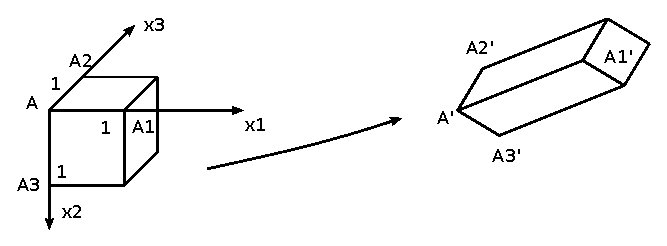
\includegraphics{../images/T1_Ch03-0003}
\end{center}
\begin{equation}
    \left\{
    \begin{aligned}
        A'A_1' &= \sqrt{1+2E_{11}}\\
        \left( A'A_1',\ A'A_2' \right) &= \arcsin \frac{2E_{12}}{\sqrt{1+2E_{11}}\sqrt{1+2E_{22}}}
    \end{aligned}
    \right.
    \label{eq:Ch03-019}
\end{equation}

Comme pour le tenseur des contraintes, on peut diagonaliser le tenseur des déformations, c'est-à-dire trouver un repère orthogonal où la matrice représentant $\mathbb{E}$ est diagonale, $E_1$, $E_2$ et $E_3$ sont appelés allongements
\begin{equation}
    \mathbb{E} = 
    \begin{bmatrix}
        E_1 & 0 & 0 \\
        0 & E_2 & 0 \\
        0 & 0 & E_3
    \end{bmatrix}
    \label{eq:Ch03-020}
\end{equation}
principaux.
La propriété caractéristique des axes principaux des déformations est que les glissements dans leur direction sont nuls.
Un cube unité d'arête dirieée selon les axes principaux se transforme en un parallélépipède rectange
\begin{center}
    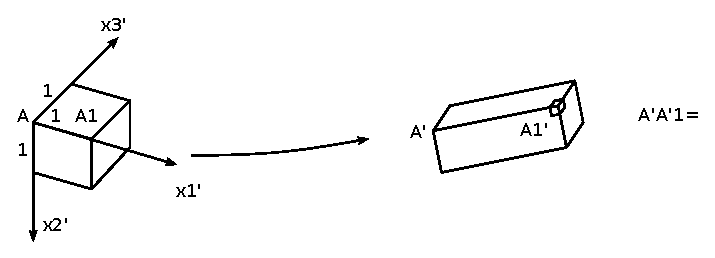
\includegraphics{../images/T1_Ch03-0004}
\end{center}

En mécanique des solides, on introduit souvent le vecteur déplacement $\vec{u} = \vec{x}-\vec{a}$, définissant le mouvement par
\begin{equation}
    x_i = a_i + u_i \left( a_1, a_2, a_3, t \right)
    \label{eq:Ch03-021}
\end{equation}
On obtient alors à partir de \eqref{eq:Ch03-022}
\begin{equation}
    F_{ij} = \delta_{ij} + \frac{\partial u_i}{\partial a_j}
    \label{eq:Ch03-022}
\end{equation}
Le tenseur des déformations est alors donné par
\begin{equation}
    E_{ij} = \frac{1}{2} \left( \frac{\partial u_i}{\partial a_j} + \frac{\partial u_j}{\partial a_i} + \frac{\partial u_k}{\partial a_i}\frac{\partial u_k}{\partial a_j} \right)
    \label{eq:Ch03-023}
\end{equation}
\section{Petites déformations} \label{sec:Ch03-2}
\subsection{Hypothèse des petites perturbations} \label{ssec:Ch03-2.1}
En Mécanique des Solides, on fait souvent l'hypothèse des petites perturbations pour laquelle le solide s'écarte peu de sa configuration de référence. Les déplacements et les déformations restent petits, ce qui a deux conséquences essentielles:
\begin{enumerate}
    \item on peut identifier variables de Lagrange $a_i$ et variables d'Euler $x_i$, dans la mesure où la différence entre les deux est négligeable.
        Ceci est tout à fait essentiel, car certaines équations s'écrivent naturellement en variables eulériennes ---les équations d'équilibre, par exemple--- alors que d'autres s'écrivent plus naturellement en variables lagrangiennes ---la définition des déformations.
        Entre autres, cela revient à écrire les équations d'équilibre dans la configuration telle qu'elle existe avant déformation, alors qu'il faudrait, en toute rigueur, les écrire dans la configuration réelle où s'appliquent effectivement les efforts.
        Cette approximation, habituellement appelée hypothèse de linéarité externe, est souvent justifiée mais on rencontrera quelques cas, en particulier toutes les questions de stabilité, où elle ne l'est pas;
    \item dans tous les calculs, on ne conserve que les termes les plus significatifs, en négligeant les termes d'ordre supérieur en $u_i$ et ses dérivées.
        En d'autres termes, on effectue une linéarisation autour de la configuration de référence, supposée naturelle, c'est-à-dire libre de contraintes, cararctérisée par 
        \begin{equation}
            \rho = \rho_c, \quad u_i = 0, \quad \sigma_{ij} = 0
            \label{eq:Ch03-024}
        \end{equation}
        et le mouvement est décrit par
        \begin{equation}
            \rho = \rho_0 + \rho, \quad u_i, \quad \sigma_{ij}
            \label{eq:Ch03-025}
        \end{equation}
        avec $\rho'$, $u_i$, $\sigma_{ij}$ petits et fonctions de $\left( x_i,t \right)$, $x_i$ représentant indifféremment les variables de Lagrange $a_i$ ou d'Euler $x_i$.
        La vitesse $V_i$ et l'accélération $\gamma_i$ sont données par
        \begin{equation}
            V_i = \frac{\partial u_i}{\partial t}, \quad \gamma_i = \frac{\partial^2 u_i}{\partial t^2}
            \label{eq:Ch03-026}
        \end{equation}
        en remarquant que les dérivées particulaires sont des dérivées partielles par rapport au temps en variables de Lagrange.
        L'équation de continuité~\eqref{eq:Ch01-011} donne
        \begin{equation*}
            \frac{\ud}{\ud t} \left( \rho_0 +\rho' \right) + \left( \rho_0 + \rho' \right) \frac{\partial V_i}{\partial x_i} = 0
        \end{equation*}
        mais  $\ud \rho_0/\ud t$, $\ud \rho' / \ud t = \partial \rho' / \partial t$ en variables de Lagrange, et on peut négliger le  terme $\rho' \partial V_i / \partial x_i$ qui est du second ordre par rapport à la perturbation.
        Il  reste  donc
        \begin{equation*}
            \frac{\partial \rho'}{\partial t} + \rho_0' \frac{\partial^2 u_i}{\partial x_i \partial t} = 0
        \end{equation*}
        ou en intégrant par rapport au temps
        \begin{equation}
            \rho' = - \rho_0 \frac{\partial u_i}{\partial x_i}
            \label{eq:Ch03-027}
        \end{equation}
        la constante d'intégration étant nulle puisque dans la configuration de référence $\rho'$ et $u_i$ sont nuls.
        Nous retrouverons cette relation au paragraphe~\ref{ssec:Ch03-2.2}.
        De même, 1'équation du mouvement \eqref{eq:Ch01-015} donne
        \begin{equation}
            \rho_0 \frac{\partial^2 u_i}{\partial t^2} = \frac{\partial \sigma_{ij}}{\partial x_j} + f_i
            \label{eq:Ch03-028}
        \end{equation}
\end{enumerate}
En particulier, on constate que $\rho'$ disparaît disparaît de l'équation du mouvement.
En Mécanique des Solides, on peut oublier l'équation de continuité qui permet seulement de calculer $\rho'$ par \eqref{eq:Ch03-027} une fois connu le déplacement $u_i \left( x_i, t \right)$.
\subsection{Tenseur linéarisé des déformations} \label{ssec:Ch03-2.2}
Dans le cadre d'hypothèse des petites perturbations, le tenseur des déformations introduit au paragraphe~\ref{ssec:Ch03-1.2} et défini par \eqref{eq:Ch03-023} à partir du déplacement $u_i$ devient
\begin{equation}
    \varepsilon_{ij} = \frac{1}{2} \left( \frac{\partial u_i}{\partial x_j} + \frac{\partial u_j}{\partial x_i} \right)
    \label{eq:Ch03-029}
\end{equation}
Ce tenseur $\varepsilon_{ij}$ est le tenseur des déformations linéarisées.
En grandes déformations, en effet, le tenseur de Green-Lagrange que nous avons défini, n'est pas le seul possible, et on peut en introduire bien d'autres, mais en petites déformations, tous ces tenseurs se réduisent au tenseur $\mathbb{\varepsilon}$ défini par~\eqref{eq:Ch03-029}.
Par linéarisation des formules \eqref{eq:Ch03-015} et \eqref{eq:Ch03-016}, il permet de calculer l'allongement dans une direction $\vec{n}$ le glissement dans deux directions $\vec{m}$ et $\vec{n}$ par les formules
\begin{equation}
\varepsilon (\vec{n}) = \varepsilon_{ij} n_i n_j\quad\text{et}\quad\gamma(\vec{m},\vec{n}) = 2 \varepsilon_{ij} n_i m_j \label{eq:Ch03-031} 
\end{equation}
obtenues simplement par développement limité des diverses fonctions internenant dans \eqref{eq:Ch03-015} et \eqref{eq:Ch03-016}.
On obtient aussi la signification des composantes $\varepsilon_{ij}$
\begin{equation}
    \varepsilon (\vec{e}_1) = \varepsilon_{11} = \frac{\partial u_1}{\partial x_1} \quad\text{et}\quad 
    \gamma (\vec{e}_1,\vec{e}_2) = \gamma_{12} = 2 \varepsilon_{12} = \left( \frac{\partial u_1}{\partial x_2} + \frac{\partial u_2}{\partial x_1} \right) \label{eq:Ch03-033}
\end{equation}
Pour dégager la signification de ce tenseur, on peut considérer le mouvement du voisinage d'un point $M$ on peut écrire
\begin{align*}
    \left( \overrightarrow{M'M_t'} \right)_i &= u_i \left( x + \ud x \right) \\
    &= u_i (x) + \frac{\partial u_i}{\partial x_j} (x) \ud x_j\\
    &= u_i + U_{i,j} \ud x_j
\end{align*}
On décompose alors $u_{i,j}$ en partie symétrique et antisymétrique
\begin{equation*}
    \left( \overrightarrow{M'M_t'} \right)_i = u_i + \omega_{ij} \ud x_j + \varepsilon_{ij} \ud x_j
\end{equation*}
\begin{equation}
    \varepsilon_{ij} = \frac{1}{2} \left( u_{i,j} + u_{j,i} \right), \quad \omega_{ij} = \frac{1}{2} \left( u_{i,j} - u_{j,i} \right)
    \label{eq:Ch03-034}
\end{equation}
On introduit le vecteur $\vec{\omega}$, adjoint du tenseur antimétrique $\omega_{ij}$ (Annexe~\ref{Ann:A}) par
\begin{equation}
    \omega_{ij} =
    \begin{bmatrix}
        0 & \omega_{12} & \omega_{13} \\
        \omega_{21} & 0 & \omega_{23} \\
        \omega_{31} & \omega_{32} & 0
    \end{bmatrix}
    =
    \begin{bmatrix}
        0 & -\omega_{3} & \omega_{2} \\
        \omega_{3} & 0 & -\omega_{1} \\
        -\omega_{2} & \omega_{1} & 0
    \end{bmatrix}
    \label{eq:Ch03-035}
\end{equation}
ce qui permet d'écrire pour $\omega_{ij} \ud x_j$
\begin{equation}
    \begin{bmatrix}
        0 & -\omega_{3} & \omega_{2} \\
        \omega_{3} & 0 & -\omega_{1} \\
        -\omega_{2} & \omega_{1} & 0
    \end{bmatrix}
    \begin{bmatrix}
        \ud x_1 \\
        \ud x_2 \\
        \ud x_3
    \end{bmatrix}
    =
    \begin{bmatrix}
        \omega_2 \ud x_3 - \omega_3 \ud x_2 \\
        \omega_3 \ud x_1 - \omega_1 \ud x_3 \\
        \omega_1 \ud x_2 - \omega_2 \ud x_1
    \end{bmatrix}
    \begin{bmatrix}
        \omega_1 \\
        \omega_2 \\
        \omega _3
    \end{bmatrix}
    \wedge 
    \begin{bmatrix}
        \ud x_1 \\
        \ud x_2 \\
        \ud x_3
    \end{bmatrix}
    \label{eq:Ch03-036}
\end{equation}
et finalement on a
\begin{equation}
    \overrightarrow{M'M_t'} = \underbrace{\underbrace{\vec{u}}_{\text{translation}} + \underbrace{\vec{\omega} \wedge \vec{\ud x}}_{\text{rotation}}}_{\text{mouvement rigidifiant}} + \underbrace{\mathbb{\varepsilon} \vec{\ud x}}_{\text{déformation pure}}
     \label{eq:Ch03-037}
\end{equation}
Le mouvement rotation et du voisinage d'un point $M$ se  compose  d'une  translation, d'une rotation et d'une déformation pure.

On peut refaire sur le tenseur des déformations tout ce que nous avons fait au chapitre~\ref{chap:Ch02} sur le tenseur des contraintes: diagonalisation, définition des invariants, décomposition en déviateur et partie sphérique
\begin{equation}
    \left\{
    \begin{aligned}
        \varepsilon_{ij} &= \mathbb{\varepsilon} \delta_{ij} + e_{ij} \\
        \varepsilon & = \frac{\varepsilon_{ii}}{3} = \frac{\varepsilon_{11} + \varepsilon_{22} + \varepsilon_{33}}{3} = \frac{\varepsilon_1 + \varepsilon_2 + \varepsilon_3}{3} \\
        e_{ij} &= \varepsilon_{ij} - \frac{1}{3} \varepsilon_{kk} \delta_{ij}, \quad e_{ii} = 0
    \end{aligned}
    \right.
    \label{eq:Ch03-038}
\end{equation}
Physiquement, cette décomposition correspond à la décomposition de la déformation en une dilatation uniforme (partie sphérique) et une distorsion, c'est-à-dire une déformation sans changement de volume (déviateur).
En effet, on vérifie facilement que la trace $\varepsilon_{ii}$ du tenseur des déformations est égale à la variation relative de volume
\begin{equation}
    \frac{\Delta V}{V} = \varepsilon_{ii} = 3\varepsilon
    \label{eq:Ch03-039}
\end{equation}
Il suffit par exemple de partir d'un élément de volume parallélépipédique orienté selon les directions principales du tenseur des déformations

Après déformation, cet élément devient un parallélépipède rectangle de côté $(1+\varepsilon_1)\ud x_1$, $(1+\varepsilon_2)\ud x_2$, $(1+\varepsilon_3)\ud x_3$ et son volume est
\begin{equation}
    V+\Delta V = (1+\varepsilon_1)(1+\varepsilon_2)(1+\varepsilon_3)\ud x_1 \ud x_2 \ud x_3 = \left[ 1 + \left( \varepsilon_1 + \varepsilon_2 + \varepsilon_3 \right) \right] V
\end{equation}
en négligeant les termes d'ordre 2 en $\varepsilon_1$, $\varepsilon_2$, $\varepsilon_3$, ce qui donne directement \eqref{eq:Ch03-039}.
La conservation de la masse
\begin{equation*}
    \left( \rho_0 + \rho' \right) \left( V + \Delta V \right) = \rho_0 V
\end{equation*}
donne alors
\begin{equation}
    \frac{\rho'}{\rho_0} = - \frac{\Delta V}{V} = - \varepsilon_{ii} = - u_{i,i}
    \label{eq:Ch03-040}
\end{equation}
et on retrouve \eqref{eq:Ch03-027}.
Nous terminons ce paragraphe par quelques exemples de déformatjons homogènes.
\begin{enumerate}
    \item Dilatation uniforme
        \begin{equation}
            \left\{
            \begin{aligned}
                u_i &= \alpha x_i \\
                \varepsilon_{ij} &= u_{i,j} = \alpha \delta_{ij}, \quad \frac{\Delta V}{V} = 3\alpha
            \end{aligned}
            \right.
            \label{eq:Ch03-041}
        \end{equation}
    \item Extension simple
        \begin{equation}
            \left\{
            \begin{aligned}
                u_1 &= \alpha x_1 \\
                u_2 &= -\beta x_2 \\
                u_3 &= -\beta x_3
            \end{aligned}
            \right. \qquad
            \mathbb{\varepsilon} = 
            \begin{bmatrix}
                \alpha & 0 & 0 \\
                0 & -\beta & 0 \\
                0 & 0 & -\beta
            \end{bmatrix}
            \label{eq:Ch03-042}
        \end{equation}
        Si cette extension se fait sans changement de volume, alors d'après \eqref{eq:Ch03-039}, on a $\beta = \frac{\alpha}{2}$.
        La décomposition en déviateur et partie sphérique s'écrit comme en \eqref{eq:Ch01-019}
        \begin{equation}
            \mathbb{\varepsilon} = \varepsilon 
            \begin{bmatrix}
                1 & 0 & 0 \\
                0 & 1 & 0 \\
                0 & 0 & 1
            \end{bmatrix}
            + e 
            \begin{bmatrix}
                1 & 0 & 0 \\
                0 & -\frac{1}{2} & 0 \\
                0 & 0 & -\frac{1}{2}
            \end{bmatrix}
            , \quad e \frac{2 \left( \alpha - \beta \right)}{3}
            \label{eq:Ch03-043}
        \end{equation}
    \item Glissement simple
        \begin{equation}
            \left\{
            \begin{aligned}
                u_1 &= \gamma x_1 \\
                u_2 &= 0 \\
                u_3 &= 0
            \end{aligned}
            \right. \qquad
            u_{i,j}' = 
            \begin{bmatrix}
                0 & \gamma & 0 \\
                0 & 0 & 0 \\
                0 & 0 & 0
            \end{bmatrix}
            \label{eq:Ch03-044}
        \end{equation}
        \begin{equation}
            \mathbb{\varepsilon} = 
            \begin{bmatrix}
                0 & \frac{\gamma}{2} & 0 \\
                \frac{\gamma}{2} & 0 & 0 \\
                0 & 0 & 0
            \end{bmatrix}, \quad
            \mathbb{\omega} = 
            \begin{bmatrix}
                0 & \frac{\gamma}{2} & 0 \\
                -\frac{\gamma}{2} & 0 & 0 \\
                0 & 0 & 0
            \end{bmatrix}, \quad
            \vec{\omega} = 
            \begin{bmatrix}
                0 \\
                0 \\
                \frac{-\gamma}{2}
            \end{bmatrix}
            \label{eq:Ch03-045}
        \end{equation}
        Le mouvement se compose de la déformation définie par $\varepsilon$ et d'une rotation de $\frac{-\gamma}{2}$ autour de l'axe $x_3$.

        Pour visualiser les déformations, on a représenté des déformations importantes, mais il ne faut pas oublier que les déformations sont en fait petites: $\alpha$, $\beta$, $\gamma$ sont des quantités petites.
\end{enumerate}
\subsection{Dualité contraintes--déformations} \label{ssec:Ch03-2.3}
On remarque l'analogie entre le tenseur des déformations $\varepsilon_{ij}$, défini par \eqref{eq:Ch03-029} à partir du déplacement $u_i$ et le tenseur des taux de déformations $D_{ij}$ défini par \eqref{eq:Ch01-023} à partir des vitesses $V_i$.
Tout ce que nous avons fait au paragraphe~\ref{ssec:Ch03-2.2} sur le petit déplacement $u_i$, en particulier toutes les interprétations physiques, peut se transposer directement aux vitesses $V_i$ qui représentent le déplacement infinitésimal entre la configuration à l'instant $t$ et celle à l'instant $t+\ud t$.
Plus précisément, on a l'analogie suivante
\begin{center}
    \begin{tabular}[c]{lccr}
        Déplacements & $u_i$ & $V_i$ & Vitesses \\
        gradient des déplacements & $u_{i,j}$ & $V_{i,j}$ & gradient des vitesses \\
        tenseur des déformations & $\varepsilon_{ij}$ & $D_{ij}$ & tenseur des taux de déformation \\
        tenseur des rotations & $\omega_{ij}$ & $\Omega_{ij}$ & tenseur taux de rotation \\
        vecteur rotation & $\vec{\omega}$ & $\vec{\Omega}$ & vecteur taux de rotation \\
        allongement dans la direction $\vec{n}$ & $\varepsilon (\vec{n})$ & & taux d'allongement \\
        glissement dans les directions $\vec{m}$, $\vec{n}$ & $\gamma (\vec{m},\vec{n})$ & & taux de glissement \\
        etc.
    \end{tabular}
\end{center}

Réciproquement, tout ce que nous avons fait au paragraphe~\ref{ssec:Ch03-1.2} peut se transposer directement en termes de déplacements.
Il s'agit simplement d'un changement de terminologie.
On parle de déplacement virtuel ${\mathop{u}^{*}}_i$ au lieu de vitesses virtuelles ${\mathop{V}^{*}}_i$ et de \emph{travaux virtuels} au lieu de \emph{puissances virtuelles}.
Par exemple, \eqref{eq:Ch01-024} ou \eqref{eq:Ch01-038} peut s'écrire
\begin{equation}
    \iiint_{\Omega} \rho \gamma_i {\mathop{u}^*}_i \ud v = \iiint_{\Omega} f_i {\mathop{u}^*}_i \ud v + \iint_{\partial \Omega} T_i {\mathop{u}^*}_i \ud S - \iiint_{\Omega} \sigma_{ij} {\mathop{\varepsilon}^*}_{ij} \ud v
    \label{eq:Ch03-046}
\end{equation}
expression du théorème des travaux virtuels ou du principe des travaux virtuels, suivant le point de vue que l'on adopte.

En particulier, le travail des efforts intérieurs par unité de volume est
\begin{equation}
    {\mathop{w}^*}_{int} = \sigma_{ij} {\mathop{\varepsilon}^*}_{ij}
    \label{eq:Ch03-047}
\end{equation}
qui met en dualité le tenseur des contraintes $\sigma_{ij}$ que nous avons étudié au chapitre~\ref{chap:Ch02}, et le tenseur des déformations $\varepsilon_{ij}$ que nous venons d'introduire.
C'est une propriété tout à fait universelle: dans toute théorie des milieux continus, il y a dualité entre les contraintes et les déformations, c'est-à-dire entre la schématisation des efforts intérieurs et la description cinématique.

Dans le cadre de la MMC classique, que nous développons actuellement, cela n'apporte qu'une simple vérification.
Dans d'autres cas, où la schématisation à adopter est moins évidente, cela sera pour nous un guide précieux.

On peut pousser plus loin cette dualité, en remarquant que dans toute théorie des milieux continus, on travaille sur quatre espaces:
\begin{itemize}
    \item l'espace des déplacements, $\mathcal{U}$,  $u \in \mathcal{U}$
    \item l'espace des déformations, $\mathcal{D}$, $\varepsilon \in \mathcal{D}$
    \item l'espace des contraintes, $\mathcal{S}$,  $\sigma \in \mathcal{S}$
    \item l'espace des chargements, $\mathcal{C}$, $\phi = \left( f_i, T_i^e \right) \in \mathcal{C}$
\end{itemize}
Le travail des efforts extérieurs met en dualité $\mathcal{U}$ et $\mathcal{C}$ par
\begin{equation}
    \langle u, \phi \rangle = \iiint_{\Omega} u_i f_i \ud v + \iint_{\partial \Omega} u_{i} T_i^e \ud S
    \label{eq:Ch03-048}
\end{equation}
Le travail des efforts intérieurs met en dualité $\mathcal{D}$ et $\mathcal{S}$ par
\begin{equation}
    \langle\langle \varepsilon, \sigma \rangle\rangle = \iiint_{\Omega} \sigma_{ij} \varepsilon_{ij} \ud v
    \label{eq:Ch03-049}
\end{equation}
et, en statique, le théorème des travaux virtuels \eqref{eq:Ch03-046} peut s'écrire
\begin{equation}
    \langle\langle \mathop{\varepsilon}^* , \sigma \rangle \rangle = \langle \mathop{u}^* , \phi \rangle
    \label{eq:Ch03-050}
\end{equation}
Nous reviendrons sur cette dualité lorsque nous parlerons des méthodes variationnelles auchapitre \ref{chap:Ch09}.
\section{Compatibilite des déformations} \label{sec:Ch03-3}
Connaissant le champ des déplacements $u_i (x)$, on en déduit par~\eqref{eq:Ch03-029}, le champ des déformations $\varepsilon_{ij}(x)$.
Réciproquement, si on connaît le champ des déformations $\varepsilon_{ij}(x)$, peut-on calculer le champ des déplacements $u_i (x)$ ? Et si oui, comment?

Le premier problème est celui de la compatibilité des déformations, le second celui de l'intégration d'un champ de déplacements.
Ce problème est extrêmement important en mécanique des solides, car nous verrons que la solution s'obtient souvent sous forme d'un champ de déformation; il faut alors remonter aux déplacements.
Remarquons que, en vertu de l'analogie discutée au paragraphe~\ref{ssec:Ch03-2.3}, on pourra transposer tous nos résultats en termes de vitesse et de taux de déformation, le problème étant alors de calculer le champ des vitesses à partir de la valeur en tout point du tenseur taux de déformation.
\subsection{Calcul de la rotation} \label{ssec:Ch03-3.1}
Pour calculer le déplacement $u_i$, il faut intégrer les formes différentielles 
\begin{equation}
    \ud u_i = u_{i,j} \ud x_j = \left( \varepsilon_{ij} + \omega_{ij} \right) \ud x_j
    \label{eq:Ch03-051}
\end{equation}
Or, on connaît $\varepsilon_{ij}(x)$ mais on ne connaît pas $\omega_{ij}$.
La première étape consiste donc à calculer la rotation $\omega_{ij}$.
\begin{lem} \label{lem:Ch03-1}
    Les dérivées de la rotation sont liées à celles de la déformation par la relation
    \begin{equation}
        \omega_{ij,l} = \varepsilon_{il,j} - \varepsilon_{jl,i}
        \label{eq:Ch03-052}
    \end{equation}
\end{lem}
\begin{proof}
    On part de la définition 
    \begin{align*}
        \omega_{ij} &= \frac{1}{2} \left( u_{i,j} - u_{j,i} \right) = \frac{1}{2} \left( u_{i,jl} - u_{j,il} \right) = \frac{1}{2} \left( u_{i,jl} + u_{l,ij} - u_{l,ij} - u_{j,il} \right) \\
        &= \frac{1}{2} \left( u_{i,l} + u_{l,i} \right)_{,j} - \frac{1}{2} \left( u_{l,j} + u_{j,l} \right)_{,i} \\
        &= \varepsilon_{il,j} - \varepsilon_{jl,i}
    \end{align*}
    en utilisant le fait que les dérivées partielles commutent: $u_{i,jl} = u_{i,lj}$, etc.
\end{proof}

On peut alors calculer la rotation $\omega_{ij}$ par intégration du système
\begin{equation}
    \ud \omega_{ij} = \left( \varepsilon_{il,j} - \varepsilon_{jl,i} \right) \ud x_l
    \label{eq:Ch03-053}
\end{equation}
\begin{lem} \label{lem:Ch03-2}
    Une condition nécessaire et suffisante pour que le système 
    \begin{equation}
        \ud f = a_l \ud x_l
        \label{eq:Ch03-054}
    \end{equation}
    soit intégrable, c'est-à-dire pour que l'on puisse calculer $f$ à partir des $a_l = f_{,l}$ est que 
    \begin{equation}
        a_{l,m} = a_{m,l}
        \label{eq:Ch03-055}
    \end{equation}
\end{lem}
\begin{proof}
    La condition nécessaire est évidente (elle exprime simplement que $f_{,lm} = f_{,ml}$).
    On démontre en mathématiques que cette condition est également suffisante.
\end{proof}

En appliquant ce lemme au système différentiel~\eqref{eq:Ch03-053}, on obtient la condition suivante
\begin{equation}
        \left( \varepsilon_{il,j} -\varepsilon_{jl,i} \right)_{,k} = \left( \varepsilon_{ik,j} - \varepsilon_{jk,i} \right)_{,l} \quad\Leftrightarrow\quad
        \varepsilon_{il,jk} + \varepsilon_{jk,il} - \varepsilon_{jl,ik} - \varepsilon_{ik,jl} = 0
    \label{eq:Ch03-056}
\end{equation}
Cette condition est une condition nécessaire et suffisante pour que l'on puisse calculer $\omega_{ij}$ à partir de $\varepsilon_{ij}$.
C'est donc une condition nécessaire pour que le champ de déformation $\varepsilon_{ij}$ soit intégrable, c'est-à-dire pour que l'on puisse calculer le déplacement $u_i$.

On tire également du Lemme~\ref{lem:Ch03-1} le résultat suivant
\begin{thm} \label{thm:Ch03-2}
    Si le champ de déformation est identiquement nul, alors le déplacement est un déplacement de solide rigide 
    \begin{equation}
        \vec{u} = \vec{c} + \vec{\omega} \wedge \vec{x}
        \label{eq:Ch03-057}
    \end{equation}
\end{thm}
Il est en effet clair que si le déplacement est un déplacement de solide rigide, infinitésimal, bien entendu, alors le tenseur des déformations associé est nul, puisque $u_{i,j}$ est antisymétrique.
Le théorème~\ref{thm:Ch03-2} constitue une réciproque.
Compte-tenu de l'analogie présentée au paragraphe~\ref{ssec:Ch03-2.3}, ce théorème est identique au Lemme~\ref{lem:Ch01-3} paragraphe~\ref{ssec:Ch01-2.1}.

\begin{proof}
    Puisque $\varepsilon_{ij}$ est nul, le Lemme~\ref{lem:Ch03-1} montre que $\omega_{ij,l}$ est nul, et donc que $\omega_{ij}$ est constant
    \begin{equation*}
        u_{i,j} = \not{\varepsilon_{ij}} + \omega_{ij} = \omega_{ij}^0
    \end{equation*}
    Le système~\eqref{eq:Ch03-051} s'intègre alors directement pour donner
    \begin{equation*}
        u_i = \omega_{ij}^0 x_j + c_{j}^0
    \end{equation*}
    que l'on peut écrire sous la forme \eqref{eq:Ch03-057} en introduisant le vecteur $\vec{\omega}$ adjoint du tenseur antisymétrique $\omega_{ij}^0$ (le calcul est le même que celui qui a conduit à \eqref{eq:Ch03-037}.
\end{proof}
\subsection{Calcul du déplacement} \label{ssec:Ch03-3.2}
Sous réserve que la condition~\eqref{eq:Ch03-056} soit vérifiée, l'intégration du système \eqref{eq:Ch03-053} donne $\omega_{ij}$ à une constante près $\omega_{ij}^0$.
Le déplacement $u_i$ s'obtiendra alors en intégrant le système \eqref{eq:Ch03-051}
\begin{equation*}
    \ud u_i = u_{i,j} \ud x_j = \left( \varepsilon_{ij} + \omega_{ij} \right) \ud x_j
\end{equation*}
Pour que cela soit possible, il faut et il suffit, d'après le Lemme~\ref{lem:Ch03-2}, que
\begin{equation*}
    \varepsilon_{ij,l} + \omega_{ij,l} = \varepsilon_{il,j} + \omega_{il,j}
\end{equation*}
Cependant, les dérivées $\omega_{ij,l}$ ont été calculées par \eqref{eq:Ch03-052}, et cette condition devient 
\begin{equation*}
    \varepsilon_{ij,l} + \varepsilon_{il,j} - \varepsilon_{jl,i} = \varepsilon_{il,j} + \varepsilon_{ij,l} - \varepsilon_{jl,i}
\end{equation*}
condition qui se trouve identiquement vérifiée, et le système \eqref{eq:Ch03-051} peut toujours s'intégrer à un déplacement de la forme 
\begin{equation*}
    \omega_{ij}^0 x_j + c_i^0
\end{equation*}
près, c'est-à-dire à un déplacement de solide rigide près.
Nous avons donc démontré le résultat suivant
\begin{thm} \label{thm:Ch03-3}
    Pour que le champ de déformation $\varepsilon_{ij}(x)$ soit intégrable, il faut et il suffit que les \emph{équations de compatibilité}~\eqref{eq:Ch03-056}
    \begin{equation*}
        \varepsilon_{il,jk} + \varepsilon_{jk,il} - \varepsilon_{jl,ik} - \varepsilon_{ik,jl} = 0
    \end{equation*}
    soient vérifiées.
    On peut alors calculer le déplacernent à un déplacement de solide près.
\end{thm}

Pratiquement, pour intégrer un champ de déformation $\varepsilon_{ij}$, c'est-à-dire pour calculer $u_i$ par résolution du système d'équations aux dérivées partielles 
\begin{equation}
    \frac{\partial u_i}{\partial x_j} + \frac{\partial u_j}{\partial x_i} = \varepsilon_{ij} (x)
    \label{eq:Ch03-058}
\end{equation}
il faut vérifier les équations de compatibilité~\eqref{eq:Ch03-056}; si elles ne sont pas vérifiées, le problème n'admet pas de solution. Si elles le sont, alors on peut  calculer le déplacement $u_i$; pour cela, on peut utiliser deux méthodes:
\begin{enumerate}
    \item méthode systématique: on intègre~\eqref{eq:Ch03-053}, puis \eqref{eq:Ch03-051};
    \item méthode directe: on calcule par résolution directe de \eqref{eq:Ch03-058} une solution particulière, et on remarque que la solution générale de \eqref{eq:Ch03-058} est la somme d'une solution particulière et de la solution générale de l'équation sans second membre, $\varepsilon_{ij} = 0$, qui, d'après le Théorème~\ref{thm:Ch03-2}, est un déplacement de solide rigide.
        Nous verrons dans la suite des exemples de cette démarche.
\end{enumerate}
Les équations de compatibilité \eqref{eq:Ch03-056} font intervenir quatre indices $i$, $j$, $k$ et $l$, variant de 1 à 3, soit \textit{a priori} 81 équations. Néanmoins, on constate que la quantité \eqref{eq:Ch03-056} est antisymétrique en $i$ et $j$, antisymétrique en $k$ et $l$, et symétrique par rapport aux couples $(i,j)$ et $(k,l)$.
Il reste donc finalement six équations indépendantes obtenues pour $ijkl = (1212),\ (1213)$, et permutation circulaire. On obtient
\begin{equation}
        \varepsilon_{11,22} + \varepsilon_{22,11} - 2 \varepsilon_{12,12} = 0 \quad\text{et}\quad
        \varepsilon_{11,23} + \left( \varepsilon_{23,1} - \varepsilon_{31,2} - \varepsilon_{12,3} \right)_{,1} = 0
    \label{eq:Ch03-059}
\end{equation}
et les qutre équations qui s'en déduisent par permutation circulaire.
On peut également obtenir un système de six équations équivalentes, en faisant $k=j$
\begin{equation}
    \begin{aligned}
        &\varepsilon_{il,kk} + \varepsilon_{kk,il} - \left( \varepsilon_{kl,ik} + \varepsilon_{ik,kl} \right) = 0 \\
        &\Delta\varepsilon_{ij} + \varepsilon_{kk,ij} - \left( \varepsilon_{jk,ik} + \varepsilon_{ik,jk} \right) = 0
    \end{aligned}
    \label{eq:Ch03-060}
\end{equation}
forme symétrique en $i,j$, qui donne donc 6 équations équivalentes à \eqref{eq:Ch03-059}.

Terminons par deux cas particuliers importants.
\begin{enumerate}
    \item Déformation homogène
        \begin{equation}
            \varepsilon_{i?} = \varepsilon_{ij}^0 = \text{Cte}
            \label{eq:Ch03-061}
        \end{equation}
        En intégrant \eqref{eq:Ch03-053}, il vient $\omega_{ij} = \omega_{ij}^0 = \text{Cte}$ et \eqref{eq:Ch03-051} donne
        \begin{equation}
            \vec{u} = \mathbb{\varepsilon}^0 \vec{x} + \vec{\omega} \wedge \vec{x} + \vec{c}
            \label{eq:Ch03-062}
        \end{equation}
    \item Déformation linéaire
        \begin{equation}
            \varepsilon_{ij} = A_{ijk} x_k
            \label{eq:Ch03-063}
        \end{equation}
        forme qui fait intervenir 18 coefficients $A_{ijk} = A_{jik}$.
        Les équations de compatibilité \eqref{eq:Ch03-059}, ne faisant intervenir que des derivées secondes de $\varepsilon_{ij}$ sont automatiquement vérifiées.
        Par intégration de \eqref{eq:Ch03-053} et \eqref{eq:Ch03-051}, on trouve
        \begin{equation}
            \begin{aligned}
                \ud \omega_{ij} &= \left( A_{ikj} - A_{jki} \right) \ud x_k \\
                \omega_{ij} &= \left( A_{ikj} - A_{jki} \right) x_k + \omega_{ij}^0
            \end{aligned}
            \label{eq:Ch03-064}
        \end{equation}
et:
        \begin{equation}
            \begin{aligned}
                \ud u_i &= \left( A_{ijk} + A_{ikj} - A_{jki} \right) x_k \ud x_j + \omega_{ij}^0 \ud x_j \\
                u_i &= \frac{1}{2} \left( A_{ijk} + A_{ikj} - A_{jki} \right) x_j x_k + \omega_{ij}^0 x_j + c_i^0
            \end{aligned}
            \label{eq:Ch03-065}
        \end{equation}
\end{enumerate}

\chapter{Lois de comportement}
\section{Problèmes de mécanique des solides} \label{sec:Ch4-1}
\subsection{Problèmes dynamiques et quasi-statiques}  \label{ssec:Ch4-1.1}
Pour résoudre un problème de Mécanique des Solides, il faut calculer la solution $(u_i, \sigma_{ij})$, c'est à dire calculer les champs de vecteurs déplacements $u_i(x)$ et de tenseurs des contraintes $\sigma_{ij}(x)$, à partir des données, qui sont constituées par
\begin{enumerate}
    \item L'ensemble des sollicitations imposées au solide
        \begin{itemize}
            \item forces volumiques
            \item conditions aux limites (forces ou déplacements imposés à la surface).
        \end{itemize}
    \item Les conditions initiales, précisant la position et la vitesse initiale du solide.
\end{enumerate}
\textbf{Exemple:} Réservoir sphérique soumis à une pression intérieure $n$
\begin{center}
    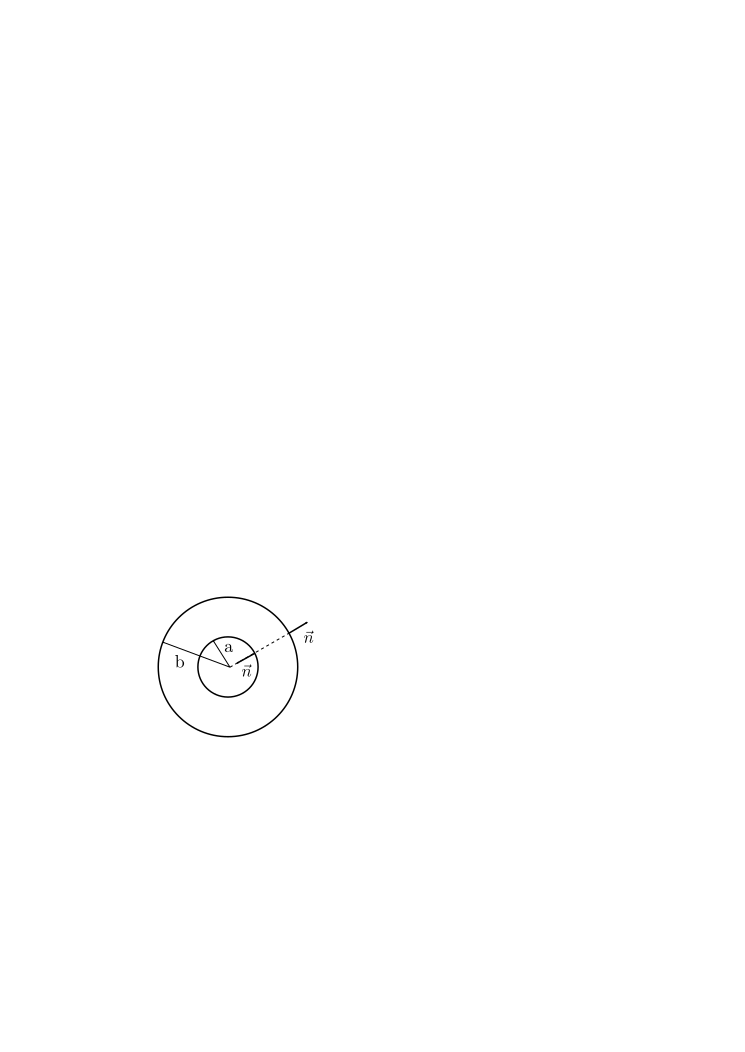
\includegraphics{../images/T1_Ch04-0001}
\end{center}
\begin{itemize}
    \item Les forces volumiques sont supposées nulles (pesanteur négligeable)
        \begin{equation}
            f_i = 0
            \label{eq:Ch04-001}
        \end{equation}
    \item La surface extérieure $r=b$ est soumise à la pression atmosphérique, la contrainte est donc nulle d'après \eqref{eq:Ch02-002}:
        \begin{equation}
            r=b \text{ : } \sigma_{ij} n_j = T_i = 0
            \label{eq:Ch04-002}
        \end{equation}
    \item La surface intérieure $r=a$ est soumise à la pression $p$ (supposée mesurée par rapport à la pression atmosphérique) d'où
        \begin{equation}
            r=a \text{ : } \sigma_{ij} n_j = T_i = -p n_i
            \label{eq:Ch04-003}
        \end{equation}
\end{itemize}
\begin{enumerate}%[a)] FIXME
    \item Problème dynamique:  On  donne  la pression  $p(t)$  comme  fonction  du  temps; on  donne  également les  conditions  initiales  -- par  exemple,  à  $t=0$,  le réservoir est au repos
        \begin{equation}
            u_i(x,0)=0 \quad V_i(x,0) = \frac{\partial u_i}{\partial t}(x,0) = 0
            \label{eq:Ch04-004}
        \end{equation}
        et on cherche la solution $u_i(x,t),\ \sigma_{ij}(x,t)$ qm doit vérifier l'équation du mouvement \eqref{eq:Ch03-028}
        \begin{equation}
            \rho_0 \frac{\partial^2 u_i}{\partial t^2} = \frac{\partial \sigma_{ij}}{\partial x_j} + f_i
            \label{eq:Ch04-005}
        \end{equation}
        avec \eqref{eq:Ch04-001}, les conditions aux limites \eqref{eq:Ch04-002} et \eqref{eq:Ch04-003}, et les conditions initiales \eqref{eq:Ch04-004}.
        Ce problème correspond par exemple à l'étude de la mise en charge brutale du réservoir.
        Moyennant une modification des conditions initiales \eqref{eq:Ch04-004}, il correspond aussi à l'étude des vibrations du réservoir, si l'on impose une pression $p(t)$ sinusoïdale
        \begin{equation}
            p(t) = p_0 \cos \omega t
            \label{eq:Ch04-006}
        \end{equation}
        on recherche alors une solution périodique en $t$, condition qui remplace \eqref{eq:Ch04-004}.
    \item Problème statique: La pression $p$ est constante c'est la pression en service du réservoir.
        On recherche alros une solution statique, c'est à dire indépendante du temps $u_i(x),\ \sigma_{ij}(x)$ vérifiant les équations d'équilibre
        \begin{equation}
            \frac{\partial \sigma_{ij}}{\partial x_j} +f_i = 0
            \label{eq:Ch04-007}
        \end{equation}
        avec \eqref{eq:Ch04-001} et les CI (conditions aux limites) \eqref{eq:Ch04-002} et \eqref{eq:Ch04-003}.
        Le temps a disparu, et les conditions initiales n'ont plus lieu d'être.
    \item Problème quasi-statique: On suppose comme en a) que la pression $t$ varie au cours du temps, $p(t)$, mais on fait l'hypothèse suivante
        \par\underline{Hypothèse quasi-statique:} Les évolutions sont suffisamment lentes pour que, dans l'équation du mouvement \eqref{eq:Ch04-005}, on puisse négliger le terme d'accélération et donc la remplacer par l'équation d'équilibre \eqref{eq:Ch04-007}.

        En d'autres termes, la sollicitation dépend du temps, mais on résoud à chaque instant un problème statique.
        Cette hypothèse est tout à fait essentielle en mécanique des solides, car elle permet de ramener à des problèmes statiques les problèmes réels qui, eux, dépendent toujours du temps.
        L'essentiel de ce cours sera désormais limité au cas où cette hypothèse est valable, l'étude des problèmes réellement dynamiques (chocs, vibrations) étant renvoyée au cours de Mécanique des Vibrations.
\end{enumerate}
\subsection{Conditions aux limites} \label{ssec:Ch4-1.2}
\textbf{Exemple 2.} Ecrasement d'un lopin entre les deux plateaux rigides d'une presse:
\begin{wrapfigure}{l}{7cm}
    \begin{center}
        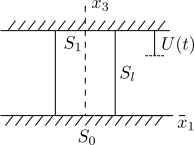
\includegraphics{../images/T1_Ch04-0002}
    \end{center}
\end{wrapfigure}
Un bloc métallique cylindrique est écrasé entre les deux plateaux rigides d'une presse.
Le plateau inférieur $x_3 =0$ est immobile, tandis que le plateau supérieur $x_3 =h$ s'enfonce d'une longueur $U(t)$.
À nouveau, on peut s'intéresser aux problèmes dynamique, statique ou quasi-statique, mais nous nous limiterons au dernier cas: la solution dépend du temps puisque la sollicitation en dépend, mais nous écrirons néanmoins les équations d'équilibre.

Comme dans l'exemple précédent, et comme dans la majorité des cas en Mécanique des Solides, la seule force de volume est la pesanteur, et nous la négligerons, d'où \eqref{eq:Ch04-001}.
La surface latérale $S_l$ est libre de contraintes
\begin{equation}
    \text{sur } S_l:\quad T_i = \sigma_{ij} n_j = 0
    \label{eq:Ch04-008}
\end{equation}
Sur les extrémités $S_0$ $(x_3=0)$ et $S_1$ $(x_3=h)$, la condition exprimant la rigidité des plateaux porte sur le déplacement vertical
\begin{equation}
    \begin{cases}
        x_3 = 0: & u_3 = 0 \\
        x_3 = h: & u_3 = -U(t)
    \end{cases}
    \label{eq:Ch04-009}
\end{equation}
mais les autres conditions aux limites dépendent des conditions de contact entre les plateaux et le lopin.

\emph{S'il n'y a pas de frottement}, c'est à dire si le contact est parfaitement lubrifié, alors la force de contact, en $x_3=h$, par
\begin{equation}
    \vec{n} = \left( 0,0,+1 \right), \quad \vec{T} = \left( \sigma_{13}, \sigma_{23}, \sigma_{33} \right)
    \label{eq:Ch04-010}
\end{equation}
doit être normale à la surface de contact.
Les conditions \eqref{eq:Ch04-009} doivent être complétées par les conditions $\sigma_{13} = \sigma_{23} = 0$
\begin{equation}
    \left\{
    \begin{aligned}
        x_3 = 0: & u_3 = 0, & \sigma_{13} = \sigma_{23} = 0 \\
        x_3 = h: & u_3 = -U(t), & \sigma_{13} = \sigma_{23} = 0
    \end{aligned}
    \right.
    \label{eq:Ch04-011}
\end{equation}

\emph{S'il n'y a pas de glissement}, c'est à dire s'il y a adhérence complète entre le lopin et le plateau, alors il faut compléter \eqref{eq:Ch04-009} par les conditions cinématiques d'adhérence $u_1 = u_2 = 0$
\begin{equation}
    \begin{cases}
        x_3 = 0: & u_1 = u_2 = u_3 = 0 \\
        x_3 = h: & u_1 = u_2 = 0, u_3 = -U(t)
    \end{cases}
    \label{eq:Ch04-012}
\end{equation}

Dans le cas réel, il y a frottement entre le plateau et le lopin, et il faut compléter \eqref{eq:Ch04-009} par la condition exprimant la loi de frottement. 
Nous adoptons la loi de frottement de Coulomb, avec un coefficient de frottement $f$,
\begin{equation}
    \left\{
    \begin{aligned}
        \vec{V} = 0 & \text{si} & |\vec{T}| < fN \\
        \vec{V} = \lambda \vec{T} & \text{si} & |\vec{T}| = fN, \lambda \geq 0
    \end{aligned}
    \right.
    \label{eq:Ch04-013}
\end{equation}
\begin{wrapfigure}{r}{4cm}
    \begin{center}
        \includegraphics{../images/T1_Ch04-0003}
    \end{center}
\end{wrapfigure}

que l'on peut encore rééecrire sous la forme
\begin{equation}
    \left\{
    \begin{aligned}
        \vec{V} = \lambda \vec{T}\\
        \lambda \geq 0, \quad fN - |\vec{T}| \geq 0, \quad \lambda \left( fN - |\vec{T}| \right) = 0
    \end{aligned}\right.
    \label{eq:Ch04-014}
\end{equation}
On obtient alors
\begin{equation}
    \left\{
    \begin{aligned}
        x_3 = 0:&\quad u_3 = 0, \frac{\partial u_1}{\partial t} =\lambda \sigma_{13}, \frac{\partial u_2}{\partial t} = \lambda \sigma_{23}, \\
            & \lambda \geq 0, -f \sigma_{33} - \sqrt{\sigma_{13}^2 + \sigma_{23}^2} \geq 0, \lambda \left( -f \sigma_{33} - \sqrt{\sigma_{13}^2 + \sigma_{23}^2} \right) = 0 \\
        x_3 = h:&\quad u_3 = -U(t), \frac{\partial u_1}{\partial t} = -\lambda \sigma_{13}, \text{etc.}
    \end{aligned}
    \right.
    \label{eq:Ch04-015}
\end{equation}

Le problème de l'écrasement d'un lopin consiste donc à trouver $u_i(x,t), \sigma_{ij}(x,t)$, vérifiant à chaque instant les équations d'équilibre \eqref{eq:Ch04-007} avec $f_i = 0$, et les conditions aux limites \eqref{eq:Ch04-008} et \eqref{eq:Ch04-011}, \eqref{eq:Ch04-012} ou \eqref{eq:Ch04-013}, suivant la nature du problème et suivant la précision des résultats cherchés: le problème \eqref{eq:Ch04-015} est certainement plus proche de la réalité que les problèmes \eqref{eq:Ch04-011} ou \eqref{eq:Ch04-012}, mais les problèmes \eqref{eq:Ch04-011} et \eqref{eq:Ch04-012} sont beaucoup plus simples, et peuvent constituer une approximation suffisante pour les besoins que l'on a.
De même, si le frottement est important, le problème \eqref{eq:Ch04-012} est certainement plus proche de la réalité qUe le problème \eqref{eq:Ch04-011}.
Néanmoins, le problème \eqref{eq:Ch04-011}, qui, comme on le verra, se résoud très simplement, peut être un approxmation suffisante, par exemple pour le calcul de la force $F$ à appliquer sur la presse et qui sera donnée par
\begin{equation}
    F(t) = - \iint_{S_0} \sigma_{33} \ud x_1 \ud x_2 = - \iint_{s_1} \sigma_{33} \ud x_1 \ud x_2
    \label{eq:Ch04-016}
\end{equation}

\textbf{Exemple 3.} Bloc pesant posé sur un plan rigide.

\begin{wrapfigure}{l}{4cm}
\begin{center}
    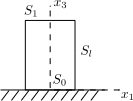
\includegraphics{../images/T1_Ch04-0004}
\end{center}
\end{wrapfigure}
Le bloc est soumis à la seule action de la pesanteur.
En notant $\rho_0 = \rho$ la masse volumique du solide, et $g$ l'accélération de la pesanteur, on a donc
\begin{equation}
    f_1 = f_2 = 0, \quad f_3 = -\rho g
    \label{eq:Ch04-017}
\end{equation}
La surface latérale $S_l$ et l'extrémité $S_1\ (x_3=h)$ sont libres de contraintes
\begin{equation}
    \left\{
    \begin{aligned}
        \text{sur } S_l & \sigma_{ij} n_j = 0 \\
        x_3 = h & \sigma_{13} = \sigma_{23} = \sigma_{33} = 0
    \end{aligned}
    \right.
    \label{eq:Ch04-018}
\end{equation}
Sur l'extrémité $S_0\ (x_3=O),$ les conditions aux limites dépendent, comme dans le cas précédent, des conditions de contact: dans le cas de non frottement on a
\begin{equation}
    x_3 = 0: \quad u_3 = 0 \quad \sigma_{13} = \sigma_{23} = 0
    \label{eq:Ch04-019}
\end{equation}
dans le cas de non glissement, on a 
\begin{equation}
    x_3 = 0: \quad u_1 = u_2 = u_3 = 0
    \label{eq:Ch04-020}
\end{equation}

\begin{wrapfigure}{l}{5cm}
    \begin{center}
        \includegraphics{../images/T1_Ch04-0005}
    \end{center}
\end{wrapfigure}
dans le cas du frottement coulombien, on a une expresslon analogue à \eqref{eq:Ch04-015}.
Toutes ces conditions supposent que le contact entre le bloc et le plan reste maintenu.
Il peut arriver -- figure ci-contre -- qu'une partie du bloc se soulève.
Il s'agit alors d'une liaison unilatérale.
La surface $S_0$ se décompose en deux zones (que l'on ne connaît pas, leur détemination fait partie du problème)
\begin{itemize}
    \item une zone de contact où l'on a
        \begin{equation}
            u_3 = 0, \quad \sigma_{33} \leq 0
            \label{eq:Ch04-021}
        \end{equation}
    \item une zone de non contact, libre de contraintes, où l'on a
        \begin{equation}
            u_3 \geq 0, \quad \sigma_{33} = 0
            \label{eq:Ch04-022}
        \end{equation}
\end{itemize}
On peut regrouper \eqref{eq:Ch04-021}, \eqref{eq:Ch04-022} en
\begin{equation}
    u_3 \geq 0, \quad \sigma_{33} \leq 0, \quad u_3 \sigma_{33} = 0
    \label{eq:Ch04-023}
\end{equation}
En supposant le contact sans frottement, il faut donc remplacer \eqref{eq:Ch04-019} par
\begin{equation}
    x_3 = 0 
    \begin{cases}
        \sigma_{13} = \sigma_{23} = 0 \\
        u_3 \geq 0, \quad \sigma_{33} \leq 0, \quad u_3 \sigma_{33} = 0
    \end{cases}
    \label{eq:Ch04-024}
\end{equation}

En toute rigueur, il aurait aussi fallu envisager cette possibilité dans l'exemple précédent, mais elle était peu plausible physiquement.

On pourrait également envisager d'autres types de conditions aux limites sur $S_0$.
\begin{wrapfigure}{l}{3cm}
    \begin{center}
        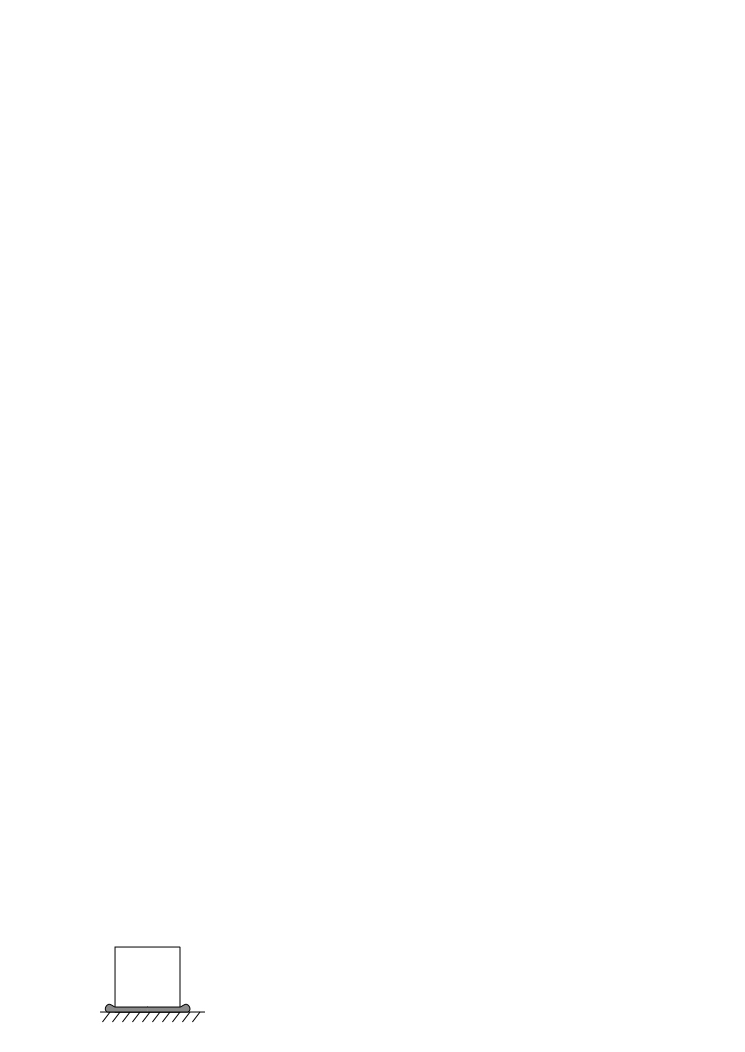
\includegraphics{../images/T1_Ch04-0006}
    \end{center}
\end{wrapfigure}
Par exemple, on peut imaginer de poser le bloc sur le plan par l'intermédiaire d'un ballon de baudruche contenant un gaz à la pression $p$.
Les efforts exercés sur le solide par le ballon se ramènent alors à une pression hydrostatique
\begin{equation}
    x_3 = 0: \quad \sigma_{33} =-p, \sigma_{13} = \sigma_{23} = 0
    \label{eq:Ch04-025}
\end{equation}

On peut déterminer $p$ en remarquant que, d'après les équations d'équilibre, les efforts exercés sur le bloc à travers $S_0$ doivent équili­brer les autres efforts appliqués, c'est à dire en l'occurence le poids du bloc.
On obtient donc la condition suivante
\begin{equation}
    -\iint_{S_0} \sigma_{33} \ud x_1 \ud x_2 = \rho g S h
    \label{eq:Ch04-026}
\end{equation}
valable quelles que soient les conditions aux limites sur $S_0$.
Avec les conditions \eqref{eq:Ch04-025}, on en tire la valeur de $p$
\begin{equation}
    p = \rho g h
    \label{eq:Ch04-027}
\end{equation}

De manière générale, dans un problème réel, l'écriture des conditions aux limites est une étape tout à fait essentielle, car d'une part ces conditions comprennent l'essentiel de la physique du problème, d'autre part elles conditionnent la facilité -- voire la possibilité -- de la résolution du problème mathématique obtenu.
Il faudra souvent faire un compromis entre la précision de la description physique et la facilité de résolution du problème mathématique.

\subsection{Lois de comportement}  \label{ssec:Ch4-1.3}
Pour résoudre un problème de mécanique des solides, if faut donc résoudre un système d'équations aux dérivées partielles.
Pour l'instant, nous avons trois équations scalaires -- les équations du mouvement~\eqref{eq:Ch04-005} ou les équations d'équilibre~\eqref{eq:Ch04-007}, suivant que l'en considère le problème dynamique ou le problème quasi-statique -- pour 9 champs inconnus: 3 composantes du déplacement $u_i(x,t)$ et 6 composantes du tenseur des contraintes $\sigma_{ij}(x,t)$.
Il manque donc 6 équations scalaires.
Ces 6 équations nous seront fournies par la ``loi de comportement'' du matériau.
Toutes les équations écrites jusqu'à présent étaient -- dans le cadre d'une schématisation donnée -- -universelles, c'est à dire indépendantes du matériau considéré.
Les équations écrites au paragraphe~\ref{ssec:Ch4-1.2} restent les mêmes pour un bloc d'acier, d'aluminium, de matière plastique, de caoutchouc, de bois, de béton, d'argile, de pâte à modeler, \ldots , sous la seule réserve que les hypothèses fondamentales soient vérifiées (théorie du premier gradient, petites déformations).

De manière générale, la loi de comportement se présente comme une ``relation'' entre le tenseur des contraintes et le tenseur des déformations.
Cette relation peut être de nature très diverse -- nous en verrons quelques exemples en~\ref{sec:Ch4-2} -- mais elle sera en général de nature ``fonctionnelle''.
À quelques cas singuliers près, nous pouvons admettre qu'elle donne le tenseur des contraintes à partir de l'histoire du tenseur des déformations -- c'est à dire de la valeur du tenseur des déforrnations à l'instant considéré et à tous les instants antérieurs -- ou bien le tenseur des déformations à partir de l'histoire du tenseur des contraintes.
\begin{equation}
    \tens{\sigma} (t) = \mathop{\tens{\sigma}}_{s=0}^{\infty} \left\{ \tens{\varepsilon} (t-s) \right\}, \quad \tens{\varepsilon} (t) = \mathop{\tens{\varepsilon}}_{s=0}^{\infty} \left\{ \tens{\sigma} (t-s) \right\}
    \label{eq:Ch04-028}
\end{equation}

Cette loi de comportement ne peut être déterminée qu'expérimentale­ment par un certain nombre ``d'essais''.
Les essais les plus faciles à interpréter sont les ``essais homogènes'' où l'on cherche à réaliser dans une éprouvette un état de contrainte et de déformation homogène.
L'exemple le plus simple est l'essai de compression simple, qui correspond à l'exemple 2 du paragraphe~\ref{ssec:Ch4-1.2}.
Si l'on cherche un état de contrainte et de déformation homogène
\begin{equation}
    \sigma_{ij} (x,t) = \sigma_{ij}(t), \quad \varepsilon_{ij}(x,t) = \varepsilon_{ij}(t)
    \label{eq:Ch04-029}
\end{equation}
alors la condition aux limites~\eqref{eq:Ch04-008} sur la surface latérale montre que toutes les composantes de $\sigma_{ij}(t)$ sont nulles, sauf $\sigma_{33}$ -- en effet, sur $S_l$ $n_3=0$ tandis que $n_1$ et $n_2$ sont quelconques -- et \eqref{eq:Ch04-016} donne $\sigma_{33}(t)=-F(t)/S$
\begin{equation}
    \tens{\sigma}(t) = \begin{bmatrix}
        0 & 0 & 0 \\
        0 & 0 & 0 \\
        0 & 0 & -F(t)/S
    \end{bmatrix}
    \label{eq:Ch04-030}
\end{equation}
La loi de conportement \eqref{eq:Ch04-028} donne alors $\tens{\varepsilon}(t)$ en fonction de $F(t)$.
On obtient alors la forme générale de déplacement par \eqref{eq:Ch03-062}
\begin{equation}
    \left\{
    \begin{aligned}
        u_1 &= \varepsilon_{11} x_1 &+ \varepsilon_{12}x_2 &+ \varepsilon_{13}x_3 &+ \omega_{2}x_3 - \omega_{3} x_2 +c_1\\
        u_2 &= \varepsilon_{12} x_1 &+ \varepsilon_{22}x_2 &+ \varepsilon_{23}x_3 &+ \omega_{3}x_1 - \omega_{1} x_3 +c_2\\
        u_3 &= \varepsilon_{13} x_1 &+ \varepsilon_{23}x_2 &+ \varepsilon_{33}x_3 &+ \omega_{1}x_2 - \omega_{2} x_1 +c_3
    \end{aligned}
    \right.
    \label{eq:Ch04-031}
\end{equation}
La CL~\eqref{eq:Ch04-009} en $x_3 =0$ donne alors
\begin{equation*}
    c_3 = 0, \quad \omega_1 = -\varepsilon_{23}, \quad \omega_2 = \varepsilon_{13}
\end{equation*}
La CL~\eqref{eq:Ch04-009}  en $x_3=h$ est alors vérifiée si
\begin{equation}
    U(t) = -h \varepsilon_{33}(t)
    \label{eq:Ch04-032}
\end{equation}
et il vient
\begin{equation}
    \left\{
    \begin{aligned}
        u_1(x,t) &= \varepsilon_{11}x_1 &+ (\varepsilon_{12} - \omega_3) x_2 &+ 2\varepsilon_{13}x_3 \\
        u_2(x,t) &= (\varepsilon_{12} + \omega_3) x_1 &+ \varepsilon_{22}x_2 &+ 2\varepsilon_{23}x_3 \\
        u_3(x,t) &= -U(t) x_3/h
    \end{aligned}
    \right.
    \label{eq:Ch04-033}
\end{equation}
Et la solution définie par \eqref{eq:Ch04-030}, \eqref{eq:Ch04-033} est solution du problème associé au cas sans frottement défini par les CL \eqref{eq:Ch04-011}.
Ainsi, pour réaliser un essai de compression simple, on écrase un lopin en lubrifiant le contact, pour s'approcher au maximum des conditions de non frottement, et en imposant, par exemple, une force $F(t)$ -- essai à force imposée --, la mesure des déplacements donne alors $\tens{\varepsilon}(t)$, et permet donc de déterminer la loi de comportement pour un tenseur $\tens{\sigma}$ de la forme \eqref{eq:Ch04-030}.

Si le matériau est isotrope -- notion que nous préciserons plus tard -- alors un tenseur $\tens{\sigma}(t)$ de la forme \eqref{eq:Ch04-030} produit une déformation de la forme
\begin{equation}
    \tens{\epsilon} (t) = 
    \begin{bmatrix}
        \varepsilon_T(t) & 0 & 0 \\
        0 & \varepsilon_T (t) & 0 \\
        0 & 0 & -U(t)/h
    \end{bmatrix}
    \label{eq:Ch04-034}
\end{equation}
La déformation se réduit à un écrasement longitudinal, mesuré par $U(t)$ et une dilatation transversale que l'on mesure facilement à l'aide d'une jauge de déformation.

\subsection{Les essais 	classiques}
L'essai de compression simple est le prototype des essais homogènes.
L'idée de base est de réaliser un état de contrainte et de déformation homogène qui peut alors être déterminé par des mesures globales d'efforts et de déformation.
Pour les métaux et la plupart des solides, l'essai de base est ``l'essai de traction'', où un barreau cylindrique de longueur $l$ et de section $S$ est soumis à une force longitudinale $F$.
L'état de contrainte et de déformation a la même forme~\eqref{eq:Ch04-030}, \eqref{eq:Ch04-034} que pour l'essai de compression.

\begin{wrapfigure}{l}{3cm}
    \begin{center}
        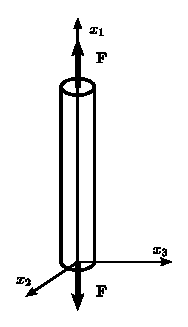
\includegraphics{../images/T1_Ch04-0007}
    \end{center}
\end{wrapfigure}
On mesure 
\begin{itemize}
    \item la force de traction $F(t)$
    \item l'allongement longitudinal $\varepsilon_{l} = \Delta l(t)/l$
    \item l'allongement transfersal $\varepsilon_T(t)$
\end{itemize}
\begin{equation}
    \tens{\sigma} =
    \begin{bmatrix}
        F(t)/S & 0 & 0 \\
        0 & 0 & 0 \\
        0 & 0 & 0
    \end{bmatrix}
    \quad
    \tens{\varepsilon} = 
    \begin{bmatrix}
        \Delta l(t)/l & 0 & 0 \\
        0 & \varepsilon_T(t) & 0 \\
        0 & 0 & \varepsilon_T(t)
    \end{bmatrix}
    \label{eq:Ch04-035}
\end{equation}

Les conditions aux limites \eqref{eq:Ch04-011} de non frottement sont pratiquement irréalisables, mais on constate expérimentalement que, pourvu que l'éprouvette soit assez longue, alors les résultats de l'essai ne dépendent pratiquement pas de la manière dont est appliquée la force $F$ , c'est à dire des conditions aux limites précises sur $S_0$ et $S_1$.
C'est le principe de Saint-Venant, sur lequel nous reviendrons au chapitre~\ref{chap:7}.

L'essai de traction est le plus simple à réaliser, mais il ne permet d'obtenir la loi de comportement que pour un tenseur des contraintes de traction ou compression simple.
Cela suffit pour déterminer complètement certaines lois de comportement, mais il est souvent nécessaire de réaliser des états de contrainte plus complexes.
Le choix est alors guidé par la possibilité technologique de réaliser un état de contrainte et déformation le plus homogène possible.
L'essai le plus couramment utilisé pour les métaux est l'essai de ``traction-torsion'' d'un tube mince.
Un tube mince de diamètre $D$, d'épaisseur $e$ et de longueur $l$ est soumis à une force longitudinale $F(t) \vec{e}_3$ et à un couple de torsion $M(t) \vec{e}_3$.

\begin{wrapfigure}{l}{3cm}
    \begin{center}
        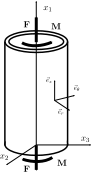
\includegraphics{../images/T1_Ch04-0008}
    \end{center}
\end{wrapfigure}
On mesure
\begin{itemize}
    \item l'allongement longitudinal $\Delta l(t)/l$
    \item l'allongement transversal $\varepsilon_T(t)$
    \item la rotation relative $\Delta \theta(t)$ des deux sections extrémités.
\end{itemize}
\endinput
tian est G2tr...nê àans le repère local (~'l..'.e.@, .e~) associé aux coorcionnées cy­

; 1 [> ,
0 0 0 0 
1 rET 
<-1 1 
(36) cr 0 0 iM/rrli e i &: 1 0 }) t:.fj/4 t • 
= ET
=1 
, i 
L 1 0 J L , ,
tMjrr n".e-FI Tf. Ti~ l 0 :Dtle/4-L M./L 
superposition d'une traction simple et d'un cisaillement simple. 
Ce type dtessai convient pour des matériaux suffisamment consistants_ En mécanique des sols, où l'on a affaire à des matériaux peu ou pas cohérents, on utilise classiquement deux types d'essais. 

Dans l'essai oediométrique, on comprlme le matériau dans un moule rigide. On réalise ainsi un état de contrainte et de déformation de la forme 

o 
(37) 
o o 



Dans l'essai "triaxial", on place une éprou­vette dans une cellule triaxiale que l'on sou­
p 
met à une pression ""fL et on superpose une, force longitudinale P On réalise ainsi un état de contrainte et de déformation de révolution (§ II.I.3) 

o 

o o 
(38) 
o o o o 
qr =
o 
Tous ces essaIS homogènes présentent l'avantage de pouvoIr s'inter­préter directement en termes de loi de comportement. Mis à part l'essai de traction, ils présentent cependant l'inconvénient d'être assez fins, nécessi­tant de grandes précautions pour obtenir des résultats significatifs. Dans la pratique courante, on utilise souvent des essais non homogènes, souvent issus de la tradition (essai pénétrornétrique en Mécanique des Sols, essai de dureté ou de résilience pour les métaux) qui permettent d'obtenir simplement des ca­ractéristiques globales du comportement. Malheureusement, ces essalS ne four­nissent sur les lois de comportement que des informations qualitatives, que l'on ne peut pas utiliser directement. 
2. COMPORTEMENT DES SOLIDES 
=========================== 
2.1 DIVERSITE DES COMPORTEMENTS 
Le but de ce paragraphe est double: d'une part nOUS allons décrire quelques uns des types de comportement que l'on peut rencontrer; d'autre part nous allons introduire la terminologie utilisée pour caractériser ces compor­tements. 
Pour les métaux à température ambiante, le comportement est convena­blement décrit par la courbe de traction, résultat de l'essai de traction. On fait croître la force F et on mesure l'allongement longitudinal 
13 
c. 
Aciers durs, métaux non ferreux
Acier doux 
-59 ­
La courbe se divise en trois régions. La région DA correspond à un comporte­
ment élastique linéaire, dont les deux caractéristiques essentielles sont: 
a) réversibilité: si, arrivé au point ~ on diminue la contrainte, on re­
descend suivant la même courbe; 
b) linéarité: la contrainte est proportionnelle à la déformation. 
Cette région correspond à la déformation réversible du réseau cristallin. 

A partir du seuil A, on entre dans la zone AB de comportement plastique, essentiellement caractérisé par son irréversibilité: si, arrivé en b on décharge, alors on redescend, non pas le long de la courbe de char­ge b A, mais sur une droite b,<,. parallèle à GA. En fait le comportement est alors à nouveau élastique tant que l'on ne redépasse pas le nouveau seuil 
b. En particulier, on constate que la déformation plastique entre A et b a eu comme effet d'élargir la région élastique. C'est le phénom~ne d'écrouÏs­sage. 
Le point B correspond à l'apparit~on de la striction instabilité géométrique qui conduit à la localisation de la déformation -. La contrainte cr diminue alors jusqu'à rupture. En fait, il s'agit de la contrainte appa­rente, càd ramenée à la surface initiale, la contrainte vraie, càd ramenée à la surface réelle de la striction, elle, continue à augmenter. De toute façon, la déformation n'est plus homogène, et cette portion de courbe ne décrit pas directement le comportement. De plus, l'hypothèse des petites dé­formations n'est plus vérifiée. 
0. 

Matériaux fragiles 
Y----------~ f L 
[0' 

En compression simple, on obtient en général un comportement symétrique DA'B' 
(mais sans striction). Pour certains matériaux fragiles (béton, fonte, roches, etc ...), cependant, on obtient en compression simple un comportement ductile, comme celui que nous avons décrit, et en traction simple, un comportement fragile conduisant à rupture très rapide. Pour les métaux·, on observe souvent l'effet Bauschinger: après une précharge OAa.. en traction, l'écrouissage qUI se traduit par une augmentation du seuil en traction, entraîne également une 
diminution du seuil en compression, alors qu'au départ les deux étaient approximativement égaux. La courbe de traction permet également de décrire le comportement d'autres matériaux, comme le caoutchouc, (comportement élastique non linéaire en première approximation) ou les sols -on représente alors I-e résultat 
cr 


caoutchouc sols 
cl 1 un essai "triaxial" à 1-fixé -qui présentent un comportement de type 
élasta-plastique avec une régibn élastique très réduite et avec ou sans plC 
suivant que le matLriau est initialement plus ou ~ins tassé. 
Pour des matériaux comme les matières plastiques ou les métaux à haute température, la courbe de traction perd toute signification, car elle dépend de manière cruciale de la vitesse de déformation. On caractérise alors le comportement par des essais de fluage et de relaxation. Pour l'essai de fluage, toujours en traction ou compression simple, on impose une contrainte constante et on observe la déformation en fonction du temps: l'application 
----­

~rance 
instantanée 
rec. différée 
déf. 
instant dU. résiduelle 

------~--------------~t 

t 
Marériau de type fluide Solide 
de la contrainte s'accompagne d'une déformation instantanée, puis la déforma­tion se poursuit, puis se stabilise, soit vers une constante, soit vers un état de fluage stationnaire à vitesse de déforr,ation constante. Si à un lns­tant to on relache la contrainte, alors la d~f0rn3tion de d&compose en trois port Lt·S: 
-une d('formation instant3nt:"·c (rcc,t.nJ\'rance ins l:-4!1tanéé), 
-une d~f(\rmation obtenue rn)lre.ssÎvCr:Jént (Y"~LOUV'r3nce différé:c), 
-une déformation résiduelle qui subsiste, cette dernière pouvant disparaître pour un matériau de type solide. 
L'essai de relaxation consiste à appliquer une déformation constant,­et à observer la contrainte nécessaire 

Fluide Solide Si l'on pousse plus loin l'essai de fluage, on voit apparaître 

l fluage primaire II fluage secondaire III fluage tertiaire 
t 
après le fluage primaire (régime transitoire) et le fluage secondaire (régime stabilisé) une zone de fluage tertiaire qui correspond au phénomène I!d'endom­rnagementll (détérioration du matériau qui conduit à la rupture). 
Ce type de comportement dépendant du temps est appelé I!viscoplasti­que l1 ou "viscoélastiquefl , selon qu'il existe ou non un seuil en dessous du­quel le comportement peut être considéré comme élastique. En première appro­ximation, les matières plastiques ont un comportement viscoélastique, et les métaux à haute température un comportement viscoplastique. 
2. 2 HODELES RHEOLOGIQUES 
Il est important de savoir construire des modèles mathématiques de comportement décrivant, au moins qualitativement, les différents types de COlT"­portement que nous venons de présenter. Les modèles rhéologiques forment une classe déjà très vaste de tels modèles. Ils s'obtiennent par combinaison de 3 modèles élémentaires 
le ressort, modèle de C(lmportement élastique 
(39) cr = Et 

-62 ­-le patin, modèle de comportement plastique 
L = 0 si \cr 1< (To 
(40) E. > 0 Si cr 
=cro
[ . 

E. < 0 Si (J = -Uo 
l' amortisseur, modèle de comportement visqueux 
'7
. 
(41 ) (J E.
= ") • TI D 
Les modèles rhéologiques s'obtiennent par montage en parallèle (les contrain­
tes s'additionnent, les deformations sont les mêmes) ou en série (les défor­
mations s'additionnent, les contraintes sont les mêmes). 
Le comportement viscoélastique peut être représenté par une combi­naison de ressorts et d'amortisseurs . 
• Par montage en série d'un ressort et d'un amortisseur, OR obtient le modèle de Maxwell: 
. 
E
cr = EL, = '7 E.J., '7. 
(42) 
{ = E
[ , + EJ., 
CVW.l~ 
L.,
ou en éliminant El.
E, et El, 
cr cr
(43 ) E 
= + 
E 
"l 
qui est la loi de comportement sous forme différentielle. Conformément à (28) 
on voit que, connaissant 1 'histoire de 0-(ou de E. ), on peut en déduire la valeur à l'instant t de E (ou de cr par intégration de l'équation dif­férentielle (43) . 
• Par montage en parallèle d'un ressort et d'un amortisseur, on obtient le 
modèle de Kelvin-Voigt 
(44) 


__ Par montage en série-d'un modèle de-Maxwell et d'un modèle de Kelvin-Voigt, on obtient le modèle de Burgers 
(45) 
[ 


En éliminant E" E.l, et E?, , il vient 
" E3 .. .. [;:;
+ _~_+_,._ CT
+ = (E 1r +
( 46) E E CT -1 CT 
"l3 E, "l:l E, "1 ,. '1:. (\,"1') 
forme différentielle de la loi de comportement. En particulier, on obtient 


en fluage' une courbe qUI représente qualitativement le comportement de certaines matières plastiques. 
L---------------~t 
Et ainsi de suite. 
Les comportements élasto-plastiques s'obtiennent par combinaison de ressorts et de patins . 
• Par montage en série d'un ressort et d'un patin, on obtient un modèle 
élasta-plastique sans écrouissage 


• On obtient un modèle avec écrouissage linéaire montage suivant 

Enfin, on peut obtenir des comportements viscoplastiques par des combinaisons des trois éléments de base. Par exemple le modèle de Bingham 

permet de décrire le comportement du goudron et de certaines pâtes. 
De manière générale, le choix d'un modèle représentant le compor­tement d'un matériau réel est un problème difficile. Le comportement des matériaux réels est complexe, et nous n'en avons présenté qu'une esquisse 
très  incomplète.  Même  pour  des  matériaux aussi  courants  que  l'acier,  de  
nombreux  aspects  du  comportement  restent mal  connus,  et  il  est  impossible  
de  construire  un  modèle .représentant  le comportement  d'un rnatérjau donné  

en toutes circonstances. Dans chaque problème, il convient de choisir le modèle le plus simple conduisant à des résultats satisfaisants pour l'uti­
lisation qu'on veut en faire. Dans certains cas, en particulier si l'on recherche une grande fiabilité, il conviendra de faire le calcul avec une loi de comportement très sophistiquée, prenant en compte tous les risques de ruine possibles, ceS calculs étant rendus possibles par les développe­ments de l'informatique. Dans d'autres cas, par contre, on pourra se satis­faire d'approximations plus grossières du comportement, et c'est la raison d'être des modèles élémentaires qui feront l'objet de la suite de ce cours. 
-65 ­Chapitre V 


\chapter{Élasticité linéaire}
\section{Description du comportement élastique} \label{sec:Ch5-1}
Le modèle de comportement le plus simple est le modèle élastique.
Pour des matériaux ayant un comportement élastoplastique ou viscoplastique, ce modèle convient parfaitement, pourvu que l'on ne dépasse pas le seuil de plasticité.
Pour des matériaux ayant un comportement de type viscoélastique, la transformation de Laplace permet de se ramener à un comportement élastique.
Même pour des matériaux ayant un comportement plus complexe, un calcul élastique peut fournir des résultats intéressants, par exemple pour le calcul des fondations en Mécanique des Sols.
Enfin, la résolution numérique d'un problème de Mécanique des Solides, avec une loi de comportement quelconque, s'effectue presque toujours par résolution d'une suite de problèmes élastiques.
Il est donc naturel, dans un cours de Mécanique des Solides, de réserver une place importante à ce modèle de comportement.

\subsection{Le tenseur d'élasticité} \label{ssec:Ch5-1.1}
Le comportement élastique est caractérisé par une relation linéaire entre contraintes et déformations.
Dans le cadre de l'élasticité tridimensionelle, cette relation s'écrit
\begin{equation}
    \begin{cases}
        \sigma_{ij} = A_{ijkh} \varepsilon_{kh}, & \varepsilon_{ij} = \Lambda_{ijkh} \sigma_{kh} \\
        \tens{\sigma} = A \left[ \tens{\varepsilon} \right], & \tens{\varepsilon} = \Lambda \left[ \tens{\sigma} \right]
    \end{cases}
    \label{eq:Ch05-001}
\end{equation}
où $A_{ijkh}$ et $\Lambda_{ijkh}$ sont les composantes de deux applications $A$ et $\Lambda$, inverses l'une de l'autre, de l'espace des tenseurs symétriques dans lui-même.
Ce sont les tenseurs d'élasticité.
Souvent $A$ est appelé tenseur de rigidité et $\Lambda$ tenseur de complaisance.
Compte-tenu de la symétrie des tenseurs des contraintes et des déformations, on doit avoir, par exemple pour $A$,
\begin{equation}
    A_{ijkh} = A_{jikh} \quad A_{ijkh} = A_{ijhk}
    \label{eq:Ch05-002}
\end{equation}

Nous ferons de plus sur ces applications les deux hypothèses suivantes
\begin{description}
    \item[Hypothèse thermodynamique.] Le tenseur d'élasticité est symétrique
        \begin{equation}
            A_{ijkh} = A_{khij}
            \label{eq:Ch05-003}
        \end{equation}
    \item[Hypothèse de stabilité.] Le tenseur d'élasticité est défini positif
        \begin{equation}
            A_{ijkh} \varepsilon_{ij} \varepsilon_{kh} \geq \alpha \varepsilon_{ij} \varepsilon_{ij}, \quad \alpha > 0
            \label{eq:Ch05-004}
        \end{equation}
\end{description}

La première hypothèse est à peu près invérifiable, malS elle con­duit à une théorie bien plus agréable et satisfaisante.
La seconde a une signification tout à fait claire, que nous verrons plus loin.
Compte-tenu des relations de symétrie \eqref{eq:Ch05-002} et \eqref{eq:Ch05-003}, on constate que le tenseur d'élasticité fait apparaître 21 coefficients.
On peut le représenter par une matrice $6\times6$ symétrique
\begin{equation}
    \begin{bmatrix}
        \sigma_{11}\\
        \sigma_{22}\\
        \sigma_{33}\\
        \sigma_{23}\\
        \sigma_{31}\\
        \sigma_{12}
    \end{bmatrix}
    =
    \begin{bmatrix}
        C_{11} & C_{11} & C_{13} & C_{14} & C_{15} & C_{16} \\
        C_{12} & C_{22} & C_{23} & C_{24} & C_{25} & C_{26} \\
        C_{13} & C_{23} & C_{33} & C_{34} & C_{35} & C_{36} \\
        C_{14} & C_{24} & C_{34} & C_{44} & C_{45} & C_{46} \\
        C_{15} & C_{25} & C_{35} & C_{45} & C_{55} & C_{56} \\
        C_{16} & C_{26} & C_{36} & C_{46} & C_{56} & C_{66}
    \end{bmatrix}
    \begin{bmatrix}
        \varepsilon_{11}\\
        \varepsilon_{22}\\
        \varepsilon_{33}\\
        \varepsilon_{23}\\
        \varepsilon_{31}\\
        \varepsilon_{12}
    \end{bmatrix}
    \label{eq:Ch05-005}
\end{equation}

On peut aussi obtenir le comportement élastique par une approche thermodynamique: un matériau élastique est un matériau sans dissipation, c'est à dire un matériau dans lequel toutes les évolutions sont réversibles.
En se plaçant d'un point de vue purement mécanique (on verra comment prendre en compte les variables thermiques au chapitre~\ref{chap:11}), l'équation~\eqref{eq:Ch01-059} donne, puisque la dissipation $\varphi$ est nulle, la relation
\begin{equation}
    \rho \frac{\ud u}{\ud t} = \sigma_{ij} \frac{\ud \varepsilon_{ij}}{\ud t}
    \label{eq:Ch05-006}
\end{equation}
(en petites déformations, $D_{ij} = \ud \varepsilon_{ij} / \ud t$).
Ceci incite à prendre l'énergie interne $u$ fonction des déformations
\begin{equation}
    \rho u = w \left( \tens{\varepsilon} \right)
    \label{eq:Ch05-007}
\end{equation}
où $w$ est le «~potentiel élastique~».
En dérivant \eqref{eq:Ch05-007} et en identifiant avec \eqref{eq:Ch05-006} on obtient
\begin{equation}
    \sigma_{ij} = \frac{\partial w}{\partial \varepsilon_{ij}}
    \label{eq:Ch05-008}
\end{equation}
Les déformations étant petites, on peut développer $w$ en série de Taylor
\begin{equation}
    w \left( \varepsilon_{ij} \right) = w_0 + \cancel{a_{ij} \varepsilon_{ij}} + \frac{1}{2} A_{ijkh} \varepsilon_{ij}\varepsilon_{kh}
    \label{<++>}
\end{equation}
où $a_{ij}$ est symétrique et où $A_{ijkh}$ vérifie les conditions de symétrie \eqref{eq:Ch05-002} et \eqref{eq:Ch05-003} qui, dans cette approche, sont automatiquement vérifiées.
En reportant dans \eqref{eq:Ch05-008} il vient
\begin{displaymath}
    \sigma_{ij} = \cancel{a_{ij}} + A_{ijkh} \varepsilon_{kh}
\end{displaymath}
qui montre que $a_{ij}$ est nul puisque la configuration de référence est supposée libre de contrainte.
On obtient donc \eqref{eq:Ch05-001}, mais avec cette approche l'hypothèse thermodynamique \eqref{eq:Ch05-003} est automatiquement vérifiée, tandis que l'hypothèse de stabilité \eqref{eq:Ch05-004} exprime le fait que l'énergie interne du matériau atteint son minimum dans l'état de référence.
C'est donc bien une hypothèse de stabilité.
En d'autres termes, il faut fournir un travail positif pour déformer le matériau à partir de son état naturel.

Nous introduisons également $\mathop{w}^{*}\left( \tens{\sigma} \right)$, transformée de Legendre de $w$
\begin{equation}
    \mathop{w}^{*}\left( \tens{\sigma} \right) = \sigma_{ij} \varepsilon_{ij} - w \left( \tens{\varepsilon} \right)
    \label{eq:Ch05-010}
\end{equation}
qui permet d'écrire
\begin{equation}
    \varepsilon_{ij} = \frac{\partial \mathop{w}^*}{\partial \sigma_{ij}}
    \label{eq:Ch05-011}
\end{equation}
Finalement, en prenant $w_0=0$, on peut réécrire la loi de comportement élastique \eqref{eq:Ch05-001} sous la forme
\begin{equation}
    \begin{aligned}
        & w = \frac{1}{2} A_{ijkh} \varepsilon_{ij} \varepsilon_{kh} = \mathop{w}^* = \frac{1}{2} \Lambda_{ijkh} \sigma_{ij} \sigma_{kh} \\
        & \sigma_{ij} \frac{\partial w}{\partial \varepsilon_{ij}} = A_{ijkh} \varepsilon_{kh} \\
        & \varepsilon_{ij} = \frac{\partial \mathop{w}^*}{\partial \sigma_{ij}} = \Lambda_{ijkh} \sigma_{kh}
    \end{aligned}
    \label{eq:Ch05-012}
\end{equation}

\subsection{Isotropie et anisotropie}
Le tenseur d'élasticité, qui caractérise complètement les propriétés élastiques du matériau, dépend, dans le cas le plus général, de 21 coefficients.
Fort heureusernent, on peut restreindre ce nombre en utilisant les symétries du matériau, c'est à dire les propriétés d'isotropie ou d'anisotropie.
Lors d'un changement de repère, les matrices $\sigma_{ij}$ et $\varepsilon_{ij}$ représentatives des tenseurs des contraintes et de déformations se transforment par \eqref{eq:Ch02-007} et \eqref{eq:Ch03-012}.
Les tenseurs d'élasticité $A$ et $\Lambda$ se transforment donc par
\begin{equation}
    A_{ijkh}' = Q_{im} Q_{jn} Q_{kp} Q_{hq} A_{mnpq}
    \label{eq:Ch05-013}
\end{equation}
Les composantes $A_{ijkh}$ du tenseur d'élasticité, ou la matrice d'élasticité \eqref{eq:Ch05-005} dépendent donc du repère choisi.
Les propriétés de symétrie matérielle caractérisent les transformations qui laissent invariantes ces composantes.

On dira qu'un matériau est isotrope si toutes ses directions sont équivalentes, c'est à dire si la matrice d'élasticité \eqref{eq:Ch05-005} est indépendante du repère choisi.
On doit donc avoir, pour tout $A_{ij}$ orthogonal,
\begin{equation}
    A_{ijkh} = Q_{im} Q_{jn} Q_{kp} Q_{kq} A_{mnpq}
    \label{eq:Ch05-014}
\end{equation}
Si, au contraire, il existe des directions privilégiées, le matériau sera dit anisotrope, et la matrice d'élasticité dépendra du repère choisi.
Il conviendra de choisir au mieux ce repère.

Pour caractériser plus précisément l'anisotropie, nous introduisons le groupe d'isotropie $\mathcal{G}$: groupe des transformations orthogonales laissant invariantes les composantes du tenseur d'élasticité.
Si l'on a choisi un repère, $\mathcal{G}$ est le groupe des matrices orthogonales vérifiant \eqref{eq:Ch05-014}.
Il est clair que $\mathcal{G}$ est un sous-groupe du groupe orthogonal.
Si $\mathcal{G}$ est le groupe orthogonal tout entier, alors le matériau est isotrope, sinon le matériau est anisotrope, et l'anisotropie est caractérisée par $\mathcal{G}$.

L'origine physique de l'anisotropie peut être liée soit à la structure du matériau, soit à son mode de formation. 

\paragraph{Anisotropie de structure}
\begin{itemize}
    \item monicristaux métalliques.
        Le groupe d'isotropie est alors le groupe cristallographique.
        Il est à noter que pour les matériaux métalliques polycristallins, habituellement considérés comme isotropes, cette isotropie est de nature statistique; le polycristal est en effet formé de la juxtaposition d'un grand nombre de grains monocristallins, donc anisotropes.
        L'isotropie globale du polycristal résulte donc du caractère aléatoire de la répartition des orientations cristallographiques de chacun des grains.
    \item matériaux composites renforcés par fibres unidirectionnelles ou multi­directionnelles -- matériaux composites stratifiés.
        Ces matériaux, de développement relativement récent, permettt d'obtenir des performances très élevées.
    \item matériaux fibreux naturels comme le bois.
\end{itemize}

\paragraph{Anisotropie de formation} pour des matériaux initialement isotropes, mais qui ont été rendus anisotropes par les traitements subis
\begin{itemize}
    \item produits métalliques semi-finis obtenus par forgeage: tôles minces obtenues par laminage et qui présentent trois directions privilégiées (direction de laminage, direction transversale et épaisseur), barres obtenues par filage et qui ont une direction privilégiée.
    \item roches ou sols de nature sédimentaire ou qUl ont subi d'importants 
tassements géologiques.
\end{itemize}

On voit donc que les manifestations de l'anisotropie sont aussi nombreuses que variées.
Nous avons présenté le concept dans le cadre de l'élasticité linéaire, mais le problème se pose pour tout comportement.
Il s'agit néanmoins d'une question difficile et encore imparfaitement comprise. 

\subsection{Élasticité anisotrope}\endinput 
Les propriétés de symétrie, décrites par le groupe d'isotropie ~ , permettent de réduire le nombre des coefficients d'élasticité. Nous allons envisager quelques cas particuliers correspondant aux types d'anisotropie que l'on rencontre le plus f~équemment en mécanique. 
a) Orthotropie. Il existe trois directions privilégiées mutuellement or[ho­gona1es, et le groupe d'isotropie est formé des symétries laissant invarian­tes chacune de ces trois directions (non orientées), càd des symétries par rapport aux axes correspondants. Si nous choisissons le repère formé par ces trois directions, alors le groupe d'isotropie ~ est formé des 4 matrices 
(15) [~::] I~ -~:] [-~ ~ ~] [-~ -~ ~l 
o 0 1 0 0 -1 0 0 -1 0 0-1 
En écrivant (14) pour ces matrices, on obtient directement la nullité des coefficients A.H1~ , A~~H ' A.1i!-~ , A~t .. ~ , etc ... , et la matrice d'élasti­cité a la forme suivante 
o:;~ 
<r.w, 0";; 
( 16) 
0;,; <r3~ <r~l, 
= 




o 

o o 
o o 
C,. o 
o o 

EH 
el,J. El, 
Et,; 
E;~ 
E.t 
Pour un matériau orthotrope, la matrice élastique ne fait plus intervenir 
que 9 coefficients. La matrice d'élasticité associée à A , inverse de (16), 
a évidemment la même structure. Bien entendu, cette forme simple est liée 
au choix du repère associé aux directions d'orthotropie. Dans un autre repère, 
cette matrice aurait une forme plus compliquée, déduite de (16) par (13). Des essais de traction sur des éprouvettes découpées dans les directions d'orthotropie permettent de déterminer assez facilement les coefficients 
Ai' A", A3' beaucoup plus difficilement les coefficients ~~~, B~~ , B.t,' 
Quant  aux  coefficients  C~,  C5  '  C"  ils sont  très diffiéiles à obtenir  
expérimentalement.  
Physiquement,  cette anisotropie s'applique par exemple  aux  tôles  

laminées ou aux matériaux composites renforcés par deux ou trois systèmes 
de fibres dans des directions perpendiculaires. 
b) Symétrie cubique. C'est un cas particulier de la précédente; il existe 
touj?UrS trois directions privilégiées mutuellement orthogonales, mais de plus ces trois directions sont équivalentes. Physiquement, cette anisotropie est celle d'un monocristal d'un matériau cubique ou cubique à face centrée. Aux matrices (15), il faut rajouter les 4 matrices suivantes 

(et celles qu'elles engendrent par produit entre elles'et avec celles de (15». On obtient alors 
r~i 1 
(j~ , 
(j~~ 1 =
(18) 
<" j
(J..~ (j~~ 
rA I!> ~ 0 0 0 
e,  A  ~  0  0  0  
B  €>  A  0  0  0  
0  0  0  C  0  0  
0  0  0  0  C  0  
0  0  0  0  0  C  

l 

€oI~ €.u 
E~~ 
El3 
EH 
E~" 
forme qui ne fait intervenir que trois coefficients A , e, et C •. 
Physiquement, cette anisotropie correspond par exemple à un matériau composite renforcé par trois systèmes de fibres identi~ues et dans des direc­tions perpendiculaires. Elle correspond aussi à un monocristal en système cu­bique ou cubique à face centrée. Plus généralement, on sait construire les matrices d'élasticité associées aux divers systèmes cristallographiques, malS ce type d'anisotropie intervient rarement en mécanique. 
c) Isotropie transverse. Le matériau a une direction privilégiée, et le groupe d'isotropie ~ est le groupe des transformations laissant invariante cette 
direction non orientée. Nous choisissons un repère ayant comme axe xla di­
3 
rection privilégiée. Le groupe ~ est alors formé: 
-71 ­-des rotations autour de x(d'angle quelconque)
3 -des symétries par rapport aux droites du plan 
xI' x2· C'est donc le groupe des matrices de la forme 
.MM, 6 ,Mmdl' 
(19) [M' [ "'l 
-~e ~e ..MM,!f -cœ'f 
0 0 0
:1 :1 
On. peut alors obtenir la forme suivante pour la matrice d'élasticité 
c:;:;~ 
<rU 
0-•• 
(20) 
<1"1.. 
(j~i 
o:.!j, 
= 

A  B  E  0  0  0  
~  A  E  0  0  0  
E  E D  0  0  0  
0  0  0  C  0  0  
0  0  0  0  c.  0  
0  0  0  0  0  A-B  

(Al 
Eu €. •• 
E1.~ 
fOi 
f~J. 
Il reste 5 coefficients d'élasticité. Les coefficients J) et E s'obtiennent par un essai de traction sur une éprouvette parallèle à la direction privilé­giée, les coefficients A et e. par un essai de traction sur une éprouvette perpendiculaire à la direction privilégiée, enfin le coefficient C peut s'ob­tenir par une expérience de torsion sur up tube minee parallèle à l'axe pri­vilégié (§ IV.I.4). C'est le type d'anisotropie que l'on rencontre le plus fréquemment: composites renforcés par fibres unidirectionnelles, composites stratifiés, bois, barres obtenues par filage, roches et sols sédimentaires, etc•.• 
2. ELASTICITE LINEAIRE ISOTROPE 
=============================== 
2.1 COEFFICIENTS D'ELASTICITE 
Pour un matériau isotrope, sans direction privilégiée, les compo­
santes, du tenseur d'élasticité doivent vérifier la relation (14) pour toute matrice orthogonale Qk! . On vérifie facilement que le tenseur 

satisfait à cette condition. Réciproquement, on peut montrer que cette con­
dition ne peut être vérifiée que si le tenseur d'élasticité a la forme (21). En écrivant (1), on obtient la loi de comportement 
(22) cr.. 
~â' 

-72 ­
ou en composantes 
[ 
0:;, = (Ât2e-) E." + Â El.+ T ÎI E~,
(23) 
= J., e-E,2­
<J:il. ce qU1 donne pour la matrice d'élasticité 
<T" 
<ftl. <f"
(24) 
crl" 
0"" O:;l. 
'" 

? ';\ 0 0 0
ÎI+~t'­
'Àtle-Â 0 0 0
" ? 0 0
'Àt-1e-0
"0 
0 0 2,e-0 0 
0 0 0 0 .le-0 
0 0 0 0

0 ~~ j 
E~, l
Etl. 
f. " 
EB 
é~, 
E,l. 
La matrice d'élasticité a la. même forme que pour un matériau à symétrie cu­
bique, avec en ~l~. la relation 
(25) C = A -~ 
c'est normal puisque l'isotropie est une restriction plus forte que la symé­
trie cubique. En fait, on peut construire (21) ou (24) en remarquant que la relation (14), vraie pour tout Q.. orthogonal, doit l'être en particulier
Â~ 
pour les Q .. (15) et (17), ce qui donne (18). La relation (25) se démontre 
~~ 
alors en prenant pour Q.. une rotation quelconque, par exemple une rotation 
4~ 
infini tésimale d'angle ete autour de xI' 
Pour calculer les coefficients Â~iit de la loi de comportement inverse, nous prenons la trace de (22) 
(L6) 

qui donne les dl!fornlàtions en f01'w~i.on des c:ontraintes par 

Ainsi, la loi élastique linéair~ isotrope générale dépend de deux cuefficients, les coefficients de Lamé :>. et e-. Paur dégager leur signifi­cation physique, et en particutier pOur ièS mes, rel', envisageons quelques états de contraintes et de déformations particuliers. 
a) Tension ou compression hydrostatique (11.17). La relation (27) donne alors 
(28) (Je . '; 0-b .. , ê .. = f. S. , cr = (')Â +.2.1;'-) E. 
~~ 
~~
'a 'a 
~I<\ = ~';\+~f;L est le module de rigidité à la compression. 
b) Glissement simple (111.44). La loi de comporte~cnL (2?') donne alors 

~~ 0 
(29) 

o 0 
o 0 
L'état de contrainte est un cisaillement simple (11.21) 
G= ~ est le module de rigidité au cisaillement ou ~dule de Coulomb. 

c) Traction simple (11.20) ou (IV.35). D'après la loi de comportement (27), 
on a 

(30) 



.avec 

{f"
cr 
= 
E 
(31 ) 

où E , module d'Young, et V, coefficient de Poisson, sont donnés par 
(32) 

, v = 

Ainsi, on peut obtenir par un essai de traction le module d'Young 
et le coefficient de Poisson: le module d'Young est la pente de la courbe de traction (qui est rectiligne dans le domaine élastique), et la mesure de la 
contraction transversale donne le coefficient de Poisson. On peut ensuite à 
partir de E et V calculer '). , ~ et K par 
E v E
(33) e-= ). = 
E 
,2, (.AtV) (.·q,V) (.-\ H» On peut également réécrire (27) avec E et \J , et il vient 

v
(34) 
E 

ou en composantes 
ê~~ = ~ [(J"~~ -V( {f"u, + (J"n)]
[ E 
(35) 
....\-1-1> -l 
=
e:1~ = -~~ -~!j,
E tG-
La matrice d'élasticité inverse de (24) peut alors s'écrire 
E•• 
ft.!. 
..j
E~. 
(36) 
= 
E. .!.~ 
E 
EH 
E.l, 
~  -'"  -)1  0  0  0  
-y  ~  -v  0  0  0  
-)1  -)1  -1  0  0  0  
0  0  0  ·H'"  0  0  
0  0  0  0  A-I-V  0  
0  0  0  0  0  .-lW  

a-~~ 
(ft.!. <r 
n 
cr.!.~ ()~t 
<r
H1 
Les coefficients d'élasticité  E ,  ::\  , e­ ,  K  , sont homogènes  
à  des contraintes,  tandis que  le coefficient de Poisson  V  est  sans  dimen­ 
sion.  Quelques valeurs  typiques de  E  et  y  sont  données  dans  le tableau  
suivant  

E (hbar) 'V 
Acie.r 22.000 0,26 -0,29 
Aluminium 7.000 0,32 -0,34 Cuivre 12.000 0,33 -0,36 Titane Il.000 0,34 
Verre 6.000 0,21 -0,27 r.aoutchouc 0,2 0,4999 ••.• 
2.2 DECOUPLAGE DEVIATEUR-PARTIE SPHERIQUE 
.La forme générale (21) du tenseur d'élasticité dans le cas isotrope présente quelques propriétés remarquables. 
Tout d'abord, cette forme (21) vérifie automatiquement l' hypothèse thermodynamique (3). C'est une des raisons pour laquelle cette hypothèse n'a pas de support expérimental, car le cas isotrope, le plus simple et le mieux connu, ne prouve rien. 
Ensuite, on remarque, par exemple sur (22) ou (34), que les direc­
tions principales des contraintes et des déformations coincident. C'est une propriété générale du comportement élastique isotrope. La relation entre con­
traintes et déformations principales est d'après (23) et (35) donnée par 

(38) 
E 

Enfin, on remarque que la loi de comportement (22) ou (34) se dé­couple en deux lois de comportement, portant la première sur les parties sphériques, la seconde sur les déviateurs -voir (11.12) et (111.38) ­
(39) 

, 

Ce découplage entre partie sphérique et déviateur est spécifique du cas iso­trope. En utilisant ce découplage, l'énergie de déformation ~ peut, d'après (12), s'écrire 
IW" " ~ 0"., f... "" i [30"f. + b·· lb.']
~ ~.·tJ J, ~ "'~ 
" i [9 Ktoi. + ~ e-e'i .e:..tJ = 1ê-li, é..ft + e-lb"'".! .e';'i 
et de même pour 

Puisque déviateurs et parties sphériques sont indépendants, on voit qu'une CNS pour que l'hypothèse de stabilité (4) soit vérifiée est que 
(50) 1<'>0 , e->o càd en utilisant (33) 
(51 ) E >0 , 


La première condition est évidente, le tableau du § 2.1 montre que pratique­ment 
(52) 0< V 
Le cas V= ~/~ est un cas limite, qui correspond aux matériaux incompressi­~. Supposons en effet que K soit très grand (par rapport à ~ et aux contraintes appliquées). La relation (39) montre alors que E1I,l' càd la variation de volume, est très petite, le matériau est donc très peu compres­sil>Ie->-~t: iL' en. r.a:isonnahle' de 'l.~app.mche:r par un _tériatt' incomprelfsiblEÇ càd soumis à la liaison 
(53) f... '"' 0 ,
...... 

Mais, par cette approximation, on perd toute information sur la partie sphé-. rique du tenseur des contraintes, la loi de comportement devient donc 
(54) 

où 1V est une pression hydrostatique arbitraite, nouvelle fonction inconnue danS la résolution d'un problème, et qui vieht compenser l'équation de liai­
son supplêmentaire (53). Une autre manière de voir les choses est d'adopter l'approche thermodynamique du § 1.1 et d'écrire à partir de (6) et (7) 

qui doit être vérifié pour taut ctE· . Idt compatible avec la liaison (53). 
~~ 
Il faut donc introduire un multiplicateur de Lagrange 1'" et il vient au lieu de (8) 
ow
(56) Dé·· "'a
= -t S·· 
""~ qui redonne (54) après développement de ~. L'apparition de cette preSS10n 
hydrostatique arbitraire est propre aux milieux incompressibles, et on la retrouve en Mécanique des Fluides. 
3. CRITERE DE LIMITE D'ELASTICITE 
================================= 
3. 1 FORNE GENERALE DU CRITERE 
On a vu au § IV.2.1 que le 
·modèle élastique représentait le com­portement des matériaux métalliques 
dans la région élastique, càd tant que 
l'on ne dépassait pas le seuil de li­
mite élastique. Pour justifier les calculs faits avec ce modèle, il faut 
donc vérifier, après avoir résolju le problème, que ce seuil n'est pas dépassé. c'est le principe du calcul élastique des structures ou des éléments de cons­truction. 
Dans le cas unidimensionnel, cette vérification se réduit à s'assu­rer que 
(57) 
lerl < O"e 
en appelant CTe. la limite .élastique en traction simple, dont la valeur est également tirée de l'essai de traction. 
Dans le cas tridimensionnel, il faut vérifier un critère de limite d'élasticité qui, de manière générale, peut s'écrire 

(58) 

où t est une fonction réelle, la fonction seuil élastique, qui limite, dans 
-77 ­
l'espace des contraintes, la région élastique dans laquelle doit rester le point représentatif des contraintes. 
Cette fonction doit vérifier les symétries du matériau, et doit donc être telle que 
(59) 


pour toute matrice Q~ orthogonale. En particulier, pour un milieu isotrope, la fonction ~ doit vérifier l'identité (59) pour toute matrice Q...& ortho­gonale. On dit alors que la fonction f est isotrope, et on montre que t 
est uniquement fonction des invariants principaux de en , ou ce qui revient au même, fonction symétrique des contraintes principales 

Plutô t que les invariants 1., 1:;,' I!> de ar définis par (II. Il), on préfè­re introduire I~, lié à la partie sphérique de or et les invariants J.I. ' Jdu déviateur de or (11.16). En effet, ces variables permettent d'obtenir
3 directement la surface seuil dans l'espace des contraintes principales 
(§ I1.2.2). En particulier, si 3n'intervient pas dans t ' alors cette sur­
3 face seuil est de révolution autour de l'axe hydrostatique. 
Pour les métaux, on a montré expérimentalement qu'une pression hy­
drostatique, aussi élevée soit-elle, ne produisait aucune déformation plasti­que. Nous pouvons donc supposer que la partie sphérique du tenseur des con­
traintes n'intervient pas dans ~ 
(61) 


Dans l'espace des contraintes principales, la surface seuil est un cylindre de génératrice parallèle à l'axe hydrostatique. Le seuil sera donc complète­ment défini par l'intersection de la surface seuil avec le plan déviatoire (§ II.2.2) ou plutôt, compte tenu des symétries, par cette intersection limi­
cr;
tée à un secteur de ~Oo, le reste étant complété par symétrie. Il va de soi que la détermination expérimentale de cette courbe est 
très difficile. 
Pour d'autres matériaux, 

en particulier pour les sols, la "pression moyenne" -<r = -~ 
alors souvent que la contrainte principale "intermédiaire" n'intervient pas 
dans 1 ' càd que ~(ï., (ï~" <r;) dépend uniquement de la plus grande et de lit plus petite des contraintes principales 

Il ressort alors du § 11.3 ..1 que, dans la représentation de Mohr, seul inter­vient le plus grand des tro~s demi-cer~les. Le critère est alors complètement 
Tt: 
défini par la "courbe intrinsèquell 
~ , enveloppe des demi-cercles li­

mites, càd correspondant à i::: 0 . 
C'est le critère de la courbe intrin­TV\..-sèque. 
3.2 CRITERES DE VON MISES ET TRtSCA 
Pour les métaux, Ou plut généralement pour les matériaux dont le critère peut s'écrire sous la forme (61), on 'utilise habituellement les cri­tères de limite d'élasticité de von Mises ou de Tresca. Le critère (61) peut s'écrire sous la forme 
(63) 


qui, d'après (11.29,30), définit i'êquation polaire de la courbe seuil dans le plan déviatoire n . Le critère le plus simple s'obtient en écrivant que )0(. ne dépend pas de J' cad, 'ljue le cylindre seuil est de révolution.
3 
Critère de von Mises 
(64) 


où X est une constante, caractêrt~tique du matériau, et que l'on peut relier à la limite élastique en traction ce . En traction simple en effet, le cri­tère (64) donne 

(J~ 
< 
soit, par comparaison avec (57), X =(Je~/3 . Le critère de von Mises s"écrit donc 
(65) 

< 

\
On peut en donner diverses interprétations physlqùes. Par exemple, (49) mon­
tre que l' énerg.ie de déformation 'l..V" se décompose en deux parties, une partie due à la dilatation, et une partie due à la distorsion, càd à la déformation 
sans changement de volume. D'après (49), le critère de von Mises exprlme que 
Ill'énergie de distorsion" ne doit pas dépasser un certain seuil 


.j
(65) 
41.'­

On peut également intr9dui'l;'illel1 &ti;4tettes octaédriques" normal es aux quatre 
:l: .. (G"... 1 	trissectt"Ïces des directions prin­cipales (ainsi nommées car elles forment un octaèdre). Les contrain­tes normale et tangentielle asso­ciées à ces facettes sont appelées contraintes normale et tangentielle octaédriques. En se plaçant en repè­

re principal, un calcul dir~Q~ontre que 

a-,+~.,..(); _~ 
~ 	:'> 
d'après (11.16). Le critère de von Mises exprime donc que la contrainte tan­
gentielle octaédriquene doit pas dépasser un certain seuil 
(67) T'cl; 
T.t:...v
.k < 
Le critère de Tresca exprime que la contrainte tangentielle ne doit 
pas dépasser un certain seuil. 
Critère de Tresca 
.... 
(68) 
T.t = 1 T.t \ -< X 
En un point donné, il faut donc vérifier que le maXlmum de la con­trainte tangentielle, lorsque la facette varie, ne dépasse pas le seuil K . 
Compte-tenu des résultats,du § II.3. l, on peut écrire cette condition 
(69) 

< x. , 

et comme pour le critère de von Mises, on obtient la valeur de ~ en identi­
fiant (69) à (57) dans le cas de la traction simple. Il vient 
(70) 

, 

Le critère de Tresca est un critère du type (62), la courbe intrinsèque étant 
TI::
la droite ~: ~/.t 

-80 ­
Les deux critères de von Mises et Tresca s'appliquent aux métaux. Ils conduisent à des rés' -1. tats légèrement différents. Par exemple, en cisail­lement simple (11.21), on obtient comme limite élastique è 
e 

pour Tresca 
(71 ) 
pour von Mises 
Dans l'espace des contraintes principales, la surface seuil est PD cylindre à base circulaire pour von Mises, hexagonale pour Tresca 

Ul. ::. 0 

La figure ci-dessus montre l'intersection de ces cylindres avec le plan dé­
viatoire n et avec le plan ~~ = 0 , description qui conviendra pour les états de contraintes planes. 
Pratiquement, ils conduisent à des résultats suffisamment voisins 
pour que, dans les applications courantes, on puisse utiliser indifférem­ment l'un ou l'autre. On utilisera donc le critère de von Mises lorsque l'on connaîtra le tenseur des contraintes par ses composantes, puisque ce critère s'exprime alors par la relation 

Ce critère se prête donc bien aux calculs analytiques ou numériques. On uti­lisera le critère de Tresca (70) lorsque l'on connaîtra a priori les direc­tions principales du tenseur des contraintes; il conduira alors à des calculs plus simples que le critère de von Mises. 

\chapter{Élasticité classique}
\section{Les équations de l'élasticité}
\subsection{Problèmes reguliers}
Pour résoudre un problème d'élasticité, il faut donc trouver un champ de déplacements $u_i\left( x,t \right)$ et un champ de contraintes $\sigma_{ij}\left( x,t \right)$ vérifiant les équations du mouvement ou d'équilibre suivant que l'on s'intéresse au problème dynamique ou quasi-statique
\begin{equation}
    \sigma_{ij,j} + f_i = \rho \frac{\partial^2 u_i}{\partial t^2} \text{ ou } 0
    \label{eq:Ch06-001}
\end{equation}
et la loi de comportement
\begin{equation}
    \sigma_{ij} = A_{ijkl} \varepsilon_{kl}
    \label{eq:Ch06-002}
\end{equation}
où le tenseur des déformations est donné par
\begin{equation}
    \varepsilon_{ij} = \frac{1}{2} \left( u_{i,j} + u_{j,i} \right)
    \label{eq:Ch06-003}
\end{equation}
On obtient donc un système de 9 équations à 9 inconnues, et le problème sera «~bien posé~», c'est à dire admettra une solution unique, pourvu qu'on lui rajoute des CL (conditions aux limites) et éventuellement des CI (conditions initiales) adéquates.
Les CI donnent la position et la vitesse du milieu à l'instant 0
\begin{equation}
    u_i \left( x,0 \right) = u_{i}^0 (x) \quad, \quad \frac{\partial u_i}{\partial t} \left( x,0 \right) = V_i^0 \left( x \right)
    \label{eq:Ch06-004}
\end{equation}

Les différents types de CL que l'on peut rencontrer ont été discutées au paragraphe~\ref{ssec:Ch4-1.2}.
On définit classiquement
\begin{description}
    \item[Problème de type I.] Les déplacements sont donnés à la frontière
        \begin{equation}
            u_i{}_{|_{\partial \Omega}} = u_i^d
            \label{eq:Ch06-005}
        \end{equation}
    \item[Problème de type II.] Les efforts appliqués au solide sur la frontière sont donnés
        \begin{equation}
            \sigma_{ij} n_j{}_{|_{\partial \Omega}} = T_i^d
            \label{eq:Ch06-006}
        \end{equation}
\end{description}
Exemples: le réservoir sphérique au paragraphe~\ref{ssec:Ch04-1.1}, ou le bloc pesant du paragraphe~\ref{ssec:Ch04-1.2} avec la CL~\eqref{eq:Ch04-025}.

Plus généralement, on a affaire à un problème mixte pour lequel sur chaque partie de $\partial \Omega$ on donne
\begin{itemize}
    \item soit les efforts, exemple \eqref{eq:Ch04-008}; 
    \item soit les déplacements, exemple \eqref{eq:Ch04-012};
    \item soit certaines composantes du déplacement et les composantes complémentaires de l'effort, exemple \eqref{eq:Ch04-011}.
\end{itemize}

Un exemple type de problème mixte est celui où l'on se donne les déplacements sur une partie de la surface et les efforts sur la partie complémentaire
\begin{equation}
    u_i{}_{|_{S_u}} =  u_i^d \quad, \quad \sigma_{ij} n_j{}_{|_{S_f}} = T_i^d
    \label{eq:Ch06-007}
\end{equation}
avec $\partial \Omega = S_u + S_f$.
C'est par exemple le cas pour les deux problèmes du paragraphe~\ref{ssec:Ch04-1.2} avec condition d'adhérence, mais pour ces mêmes problèmes avec conditions de non frottement, les CL sur les bases donnent la composante du déplacement sur $x_3$ et les composantes de l'effort sur $x_1$, $x_2$.
De manière générale, nous introduisons la classe des problèmes réguliers, problèmes pour lesquels en tout point de la frontière $\partial \Omega$ sont données 3 composantes complémentaires de l'effort $T_i = \sigma_{ij} n_j$ ou du déplacement $u_i$.
Pour qu'un problème soit régulier, il faut que l'intégrale représentant le travail des efforts de contact puisse se décomposer en deux termes
\begin{equation}
    \iint_{\partial \Omega} \sigma_{ij} n_j u_i \ud S = T_f^d \left( u_i \right) + T_u^d \left( \sigma_{ij} \right)
    \label{eq:Ch06-008}
\end{equation}
le premier terme $T_f^d$ représentant le travail des efforts donnés dans le déplacement (inconnu), et le second le travail des efforts de contact (inconnus) dans les déplacements donnés.
Pour le problème mixte \eqref{eq:Ch06-007}, on a simplement
\begin{equation}
    \iint_{\partial \Omega} \sigma_{ij} n_j u_i \ud S = \underbrace{\iint_{S_u} \sigma_{ij} n_j u_i^d \ud S}_{T_u^d\left( \sigma_{ij} \right)} +  \underbrace{\iint_{\partial \Omega} T_i^d u_i \ud S}_{T_f^d\left( u_i \right)}
    \label{eq:Ch06-009}
\end{equation}
(les problèmes de type I et II sont des cas particuliers du problème mixte~\eqref{eq:Ch06-007}).
Pour les autres problèmes réguliers, cette décomposition est plus longue à écrire.
Par exemple, pour le problème du bloc pesant avec condition de non frottement \eqref{eq:Ch06-019}, on a
\begin{equation}
    \iint_{\partial \Omega} \sigma_{ij} n_j u_i \ud S = \underbrace{\iint_{S_l +S_1} T_i^d u_i \ud S - \iint_{S_0} \left( \sigma_{13}^d u_i + \sigma_{23}^d u_2 \right.}_{T_f^d\left( u_i \right)} + \underbrace{ \left.\sigma_{33} u_3^d \right)}_{T_u^d\left(\sigma_{ij} \right)} \ud S
    \label{eq:Ch06-010}
\end{equation}
Pour ce problème particulier, chacun des termes est nul d'après \eqref{eq:Ch04-018} et \eqref{eq:Ch04-019}, mais peu importe, l'essentiel est d'examiner ce qui est donné par les conditions aux limites, et de vérifier que l'on peut effectuer la décomposition \eqref{eq:Ch06-008} sans ambiguïté.
En particulier, il en résulte que, pour le problème homogène associé, c'est à dire pour le problème correspondant à toutes les données nulles, on a automatiquement
\begin{equation}
    \iint_{\partial \Omega} \sigma_{ij} n_j u_i \ud S = 0
    \label{eq:Ch06-011}
\end{equation}
c'est un moyen commode pour vérifier qu'un problème est régulier.

Cette notion de problème régulier est essentielle, car elle recouvre la formulation naturelle des conditions aux limites en Mécanique des Solides en général.
En élasticité, les problèmes réguliers sont des problèmes linéaires -- on peut donc superposer plusieurs solutions -- et qui permettent de démontrer un certain nombre de théorèmes généraux, notamment des théorèmes d'existence et d'unicité -- un problème régulier est bien posé et les théorème~ d'énergie qui feront l'objet d'un chapitre.

Il existe des problèmes non réguliers, comme par exemple les problèmes de frottement, par exemple le problème du lopin avec la CL \eqref{eq:Ch04-015}, ou les problèmes unilatéraux, comme le problème du bloc avec la CL \eqref{eq:Ch04-024}.
Dans les deux cas, il s'agit de CL non linéaires qui rendent le problème non linéaire, et donc beaucoup plus difficile.
Les liaisons élastiques donnent un exemple de problème linéaire non régulier.
Nous rencontrerons aussi des problèmes non réguliers par manque de données, mais il s'agit alors d'une non régularité superficielle, et qui ne nous gênera guère.

\subsection{Theorème d'unicité en dynamique}
Comme nous l'avons affirmé plus haut, un problème régulier est bien 
posé, c'est à dire admet une solution unique.
A titre d'exemple, nous allons démontrer le théorème d'unicité dans le cas dynamique.
Nous partons donc d'un problème dynamique régulier.
Pour fixer les notations, nous prendrons des CL mixtes de type \eqref{eq:Ch06-007}, mais la démonstration est valable, à des difficultés de notations près, pour tout problème régulier.
Nous cherchons donc $u_i\left( x,t \right)$, $\sigma_{ij}\left( x,t \right)$, $\varepsilon_{ij}\left( x,t \right)$, solution du problème suivant
\begin{equation}
    \left\{
    \begin{aligned}
        \rho \frac{\partial^2 u_i}{\partial t^2} &= \sigma_{ij,j} + f_i \\
        \sigma_{ij} &= A_{ijkl} \varepsilon_{kh} \\
        \varepsilon_{ij} &= \frac{1}{2} \left( u_{i,j} + u_{j,i} \right) \\
        u_i \left( x,0 \right) &= u_i^c \left( x \right) \quad & V_i\left( x,0 \right) = V_i^c\left( x \right) \\
        u_i{}_{|_{S_u}} &= u_i^d  \quad & \sigma_{ij} n_j{}_{S_f} = T_i^d
    \end{aligned}
    \right.
    \label{eq:Ch06-012}
\end{equation}
Au paragraphe~\ref{ssec:Ch01-2.1} nous avons démontré le théorème de l'énergie cinétique \eqref{eq:Ch01-029}, mais en élasticité on a d'après \eqref{eq:Ch05-006} et \eqref{eq:Ch05-008}
\begin{equation}
    \sigma_{ij} D_{ij} = \sigma_{ij} \frac{\ud \varepsilon_{ij}}{\ud t} = \frac{\ud w}{\ud t}
    \label{eq:Ch06-013}
\end{equation}
ce qui permet d'écrire \eqref{eq:Ch01-029} sous la forme
\begin{equation}
    \frac{\ud}{\ud t} \left( K + W \right) = \iiint_{\Omega} f_i \frac{\partial u_i}{\partial t} \ud v + \iint_{\partial \Omega} \sigma_{ij} n_j \frac{\partial u_i}{\partial t} \ud S
    \label{eq:Ch06-014}
\end{equation}
où $W$ est l' énergie de déformation du so1ide
\begin{equation}
    W = \iiint_{\Omega} w \ud v = \frac{1}{2} \iint_{\Omega} A_{ijkh} \varepsilon_{ij} \varepsilon_{kh} \ud v
    \label{eq:Ch06-015}
\end{equation}
La signification de \eqref{eq:Ch06-014} est claire: la dérivée par rapport au temps de l'énergie totale (cinétique + de déformation) du solide est égale à la puissance des efforts extérieurs.

Supposons maintenant que notre problème \eqref{eq:Ch06-012} admette deux solutions correspondant aux mêmes données $\left( f_i, u_i^0, V_i^0, u_i^d, T_i^d \right)$.
La différence de ces deux solutions
\begin{equation}
    \bar{u}_i = u_i^{(2)} - u_i^{(1)}, \quad \bar{\varepsilon}_{ij} = \varepsilon_{ij}^{(2)} - \varepsilon_{ij}^{(1)}, \quad  \bar{\sigma}_{ij} = \sigma_{ij}^{(2)} - \sigma_{ij}^{(1)}
    \label{eq:Ch06-016}
\end{equation}
sera solution du problème homogène associé à \eqref{eq:Ch06-012}, c'est à dire du problème correspondant aux données nulles
\begin{equation}
    \bar{f}_i = 0, \quad \bar{u}_i^0 = \bar{V}_i^0 = 0, \quad \bar{T}_i^d= 0
    \label{eq:Ch06-017}
\end{equation}
En appliquant \eqref{eq:Ch06-014} à ce problème, on trouve que le second membre
\begin{equation}
    \iint_{\Omega} \bar{f}_i \frac{\partial \bar{u}_i}{\partial t} \ud v + \iint_{S_u} \bar{\sigma_{ij}} n_j \frac{\partial \bar{u}_i^d}{\partial t} \ud S + \iint_{S_f} \bar{T}_i^d \frac{\partial \bar{u}_i}{\partial t} \ud S = 0
    \label{eq:Ch06-018}
\end{equation}
est nul d'après \eqref{eq:Ch06-017} , puisque $\bar{f}_i$, $\bar{T}_i^d$ et $\bar{u}_i^d$ et donc $\partial \bar{u}_i^d/\partial t$ sont nuls.
On en tire
\begin{equation}
    \frac{\ud}{\ud t} \left( \bar{K} + \bar{W} \right) = 0, \quad \bar{K} + \bar{W} = \text{Cte} = 0
    \label{eq:Ch06-019}
\end{equation}
puisqu'à l'instant initial on a d'après \eqref{eq:Ch06-017}
\begin{equation}
    \bar{u}_i \left( x,0 \right) = \frac{\partial \bar{u}_i}{\partial t} \left( x,0 \right) = 0
    \label{eq:Ch06-020}
\end{equation}
Or l'énergie cinétique $K$, par définition, et l'énergie de déformation $W$ d'après le postulat de stabilité \eqref{eq:Ch04-004}, sont définis positifs, d'où il résulte que $\bar{K}$ et $\bar{W}$ restent nuls au cours du temps.
On a donc en tout point et à tout instant $\partial \bar{u}_i/\partial t = 0$ d'où l'on tire
\begin{equation}
    \bar{u}_i \left( x,t \right) = 0, \quad u_i^{(2)} \left( x,t \right) = u_i^{(1)} \left( x,t \right)
    \label{eq:Ch06-021}
\end{equation}
Les deux solutions coïncident et le problème \eqref{eq:Ch06-012} a une solution unique.
Nous démontrerons au chapitre \ref{chap:09} le théorème d'unicité peur le problème statique, mais provisoirement nous l'admettrons.

\subsection{Équations de Navier}
Pour résoudre analytiquement un problème d'élasticité, on postule \textit{a priori} une forme particulière pour la solution, et on essaie de vérifier toutes les équations.
Si on y parvient, alors d'après le théorème d'unicité pour un problème régulier, c'est la solution du problème.
Il en résulte donc deux méthodes, suivant que l'on essaie un champ de déplacement ou un champ de contraintes.

Si l'on part du champ de déplacement $u_i$ on peut calculer le tenseur des déformations par \eqref{eq:Ch06-003} et le tenseur des contraintes par la loi de comportement \eqref{eq:Ch06-002}.
Il ne reste donc plus à vérifier que les équations du mouvement \eqref{eq:Ch06-001}, les conditions aux limites de type déplacement et de type effort et éventuellement les conditions initiales.
Si on reporte \eqref{eq:Ch06-002} et \eqref{eq:Ch06-003} dans l'équation du mouvement \eqref{eq:Ch06-001}, on obtient l'équation qui doit être vérifiée par le champ de déplacements $u_i\left( x,t \right)$ en dynamique ou $u_i(x)$ en statique
\begin{equation}
    A_{ijkh} \frac{\partial^2 u_k}{\partial x_j \partial x_h} + f_i = \rho \frac{\partial^2 u_i}{\partial t^2} \text{ ou } 0
    \label{eq:Ch06-022}
\end{equation}
où on a utilisé la symétrie \eqref{eq:Ch05-003} de $A_{ijkh}$ et en supposant le matériau homogène ($A$ constant).
En élasticité, le temps n'intervient pas dans la loi de comportement.
Il n'intervient donc que dans l'équation du mouvement et disparaît donc en quasi-statique à l'exception des problèmes de frottement, où il reste dans la CL \eqref{eq:Ch04-015}.
Ainsi en élasticité, on ne parle jamais de problèmes quasi-statiques, mais uniquement de problèmes statiques.
Pour résoudre un problème quasi-statique, il suffit en effet de résoudre à chaque instant le problème statique correspondant.
Nous n'envisagerons plus désormais que le cas statique.

Dans le cas de l'élastictté linéaire isotrope -- élasticité classique -- l'équation \eqref{eq:Ch06-022} devient d'après \eqref{eq:Ch05-023}, et en nous limitant au cas statique
\begin{equation}
    \left( \lambda + \mu \right) u_{i,ik} + \mu u_{i,kh} + f_i = 0
    \label{eq:Ch06-023}
\end{equation}
soit, en introduisant les opérateurs de l'analyse vectorielle (Annexe~\ref{Ann:A})
\begin{equation}
    \left( \lambda + \mu \right) \grad \left( \dive \vec{u} \right) + \mu \Delta \vec{u} + \vec{f} = 0
    \label{eq:Ch06-024}
\end{equation}
ou de manière équivalente
\begin{equation}
    \left( \lambda + 2\mu \right) \grad \dive \vec{u} - \mu \rot \rot \vec{u} + \vec{f} = 0
    \label{eq:Ch06-025}
\end{equation}
Ces équations sont appelées les équations de Navier.
Elles traduisent les équations d'équilibre pour le champ des déplacements.

Ainsi la première méthode de résolution d'un problème d'élastostatique consiste à 
\begin{itemize}
    \item postuler un champ de déplacements;
    \item vérifier les équations de Navier \eqref{eq:Ch06-024} ou \eqref{eq:Ch06-025};
    \item vérifie, les CL de type déplacement;
    \item vérifier les CL de type effort.
\end{itemize}
Pour postuler le champ de déplacements, on s'inspire habituellement des CL de type déplacement et des symétries.
On verra des exemples de cette méthode au \ref{ssec:Ch06-2.2} et au paragraphe~\ref{ssec:Ch07-2.1}. 

Si on prend la divergence de l'équation \eqref{eq:Ch06-025}, on obtient l'équation de la dilatation
\begin{equation}
    \left( \lambda + 2 \mu \right) \Delta \left( \dive \vec{u} \right) + \dive \vec{f} = 0
    \label{eq:Ch06-026}
\end{equation}
qui nous sera utile plus loin.

\subsection{Équations de Beltrahi}
\endinput
La seconde méthode de résolution consiste à postuler un champ de contraintes. La loi de comportement permet alors de calculer le champ des défotmations, mais pour pouvoir calculer le vecteur déplacement, il faut que Ce champ de déformations soit compatible (§ 111.3). Ainsi le champ de contraintes choisi doit vérifier les équations d'équilibre et un système d'équations traduisant les équations de compatibilité. Nous allons obtenir ce Système d'équations dans le cas statique et en élasticité classique et homOgène. 
Nous partons des équations de compatibilité sous la forme (111.60) et de la loi de comportement sous la forme (V.34). On obtient ainsi 
À -~y
(~G -" "~r" S . ) + <TU, ..
E Ai 
E .~ J~e E )..,~ 
.A +>! 2\l 
( ()iç.,:d.,+ ().<.~, i~ ) + -cru. .. = 0 
)J,o~
E E 
s..
(...J +v) O:t,~t -li O"H te ~a + <r~. .' 
) "'"', ""cl 
-(-1+"') [<Jit.,h + <T.i.,,-,i~ ] = o 
mais d'après les équations d'équilibre \eqref{eq:Ch06-001} 

et; 4'après la loi de comportement (V.34) et l'équation de la dila ta tion \eqref{eq:Ch06-026} 
E E 
= ­
(J.U.,U = éU,U t,À.
--l-~y (:;\ + ~t'")(-1-~)l) 
•
SOle finalement avec (V. 33) 

.A +Ii
\eqref{eq:Ch06-029} 
= ­
.-1-v 
En teportant \eqref{eq:Ch06-028} et \eqref{eq:Ch06-029} dans \eqref{eq:Ch06-027} on obtient 
(30) 

+ 

+ 

= 0 
Ces équations sont appelées équations de Beltrami, et elles traduisent les équations de compatibilité pour les contraintes. Si les forces de volume sont nulles, elles se simplifient en 
(31) 

=0 

En particulier, elles seront automatiquement vérifiées si les contraintes 
-88 ­
,Sont des fonctions linéaires des coordonnées. 
La seconde méthode de résolution d'un problème élasto-statique con­
siste à postuler un champ de contraintes; vérifier les équations d'équilibre; v€rifier les équations de Beltrami; vérifier les CL de type effort; 
puis, le cas échéant 
' intégrer le champ de déplacements; 

• vérifier les CL de type déplacement.
\ On voit donc que cette méthode s'applique tout naturellement aux problèmes de type II pour lesquels on peut sauter les deux dernières étapes. Nous en verrons des exemples au § 2.1 et aux § VII.2.2 et VII.3.1 . 

Comme premier exemple, on peut citer le problème de la compression d'un lopin avec CL de non frottement, qui a été résolu de manière tout à fait générale au § IV.I.3 • Nous allons traiter deux autres exemples tirés du § IV. 1 • 
2.1 DEFORMATION D'UN BLOC PESANT 
:lt~ 


Nous considérons donc le problème du bloc pesant posé sur un ballon de baudruche (§ IV.I.2). On aura donc et les CL
i.e -Pt 
sont 
(T.. 'fI.. .. 0 sur 
St
...t t 
(32) 
et& ..  <l'~\ • <l"1.~ <1"\\
'" c-O x.,. 0 <l'u • <I",!> = 0 , (TU .. -1" 
C'est un problème régulier -la solution sera donc unique -de type II, ce qui conduit à rechercher le champ de contraintes. Les trois équations d'équi­libre s'écrivent 
-89 ­
<r .. .. =-0 
-4.04 lot (J'~/~ (f.~,lo 
e
(33) 
cr-.. (f'1. 1. +-<rJ, ~ ; 0
13., ..f , , Ij + û .. = 
~~, l. a-a.,~ f''J'
A.~,"" 
Les conditions aux limites sur la surface latérale s'écrivent [;n, = (n.,,'n..t., O)J 
0-:." '1'\..1 + a-~ l, tf\.l, = 
(34 ) 1-0
(fl.< '1\., <T~~ '1\.1. =
{ 0 
a-,!~ '1\., +-= 0
0;.'" "'"l. L'examen de ces équations nous conduit à chercher le tenseur des contraintes sous la forme 

o 
(35) 
o o 

qui vérifie automatiquement' -les conditions aux 1imites \eqref{eq:Ch06-034} sur St -les conditions aux aimites portant sur~. et <T.ta en x3=0 et x=.q" •
3Les équations d'équilibre donnent alors 

et les conditions aux limites en x~=~ et x3~O donnent 

On retrouve donc (IV.27). Par ailleurs, ce champ de contraintes est linéaire, 
il vérifie donc automatiquemeQt les équations de Beltrami \eqref{eq:Ch06-031} ( €lcctL). Ainsi, le champ de contraintes \eqref{eq:Ch06-035},\eqref{eq:Ch06-036} virifie toutes les équations du pro­blème. C'est la solution. 
Si l'on veut cpnnaître le dép~acement, alors on calcule le champ de déformations par la loi de cOIDPotteUJent 
• 
_)1 rt~3 0 
-
~ 
•
(37) (. 
0 
-)1 f' t 'Jel 0
-
E 
•
0 0 r~~l 
en prenant x.~ & x-~ , càd en prenant l'origine des coordonnées sur la face
3 supérieure du bloc. Par rapport à cette nouvelle variable, le champ des dé­
-
formations est linéaire, et on peut appliquer la formule (111.65) pour le cal­
-90 ­
cul du déplacement, malS on peut aussi procéder directement à partir de \eqref{eq:Ch06-003}. 
En effet 
~
E~; 
(38) 
=
E" 
=
f H 
.2 f.(:/, 
(39) 
J­
E.. ., :l, Et, 
et on obtient 
êI..u. ~ -\ ' ../
%) E 4; ~ -P'à'X-,~ ... 'f; (tc,,!r.,t.)
=EP~"'; 
l b
'il "':~ 
'GA, , 
~-Xf~'.X\ =? E -U., E
o~. 
'O.u.,. , 
~ -~ P'à-~, => E.u.,2,'0 'X.,t. E 
Ô-U, 
'O.IL" 
~ 
= 
+ 'f-l,,2, +
Ô (JO,
" 'X.... 
'il -U., 'ô .u" = + =-v p ';} le,
'0 t;:e' 'ô 'X-,
1 
'O.u... '0-U.; 
+ =-)lP'à''X"
" 
Ô I.C~ 'Ocr:.... 
une solution part-icu.lière 
, = -V F'} 'X, /.Co + 'f.. (T,~ J 'X.~) 
, 
+
= -;J F~.lC", éC,; 'f.l, ('X~, IX-, ) 
<;0
'h,~ 0 
+ (f\~ + '\'",-1 = 0 
+ % 0
'f~,; + '\\.l, 

d'où finalement la solution, en revenant à x
3 

-VP'à'I.C,(.lC;-..l) 
(41 ) 
-V P~ r.i:" (~; -~) 
:!.. f ~ [(.x, -Ât + V (.x: +r.c;) ) 
.1, à un déplacement de solide près. 

2.2 RESERVOIR 
Nous avec et
Î:.= 0 
f 
r=a 
(42) 
l 
r=b 
Compte-tenu de blème, on peut 
On en tire l'allure de la déforma­tion du bloc. 
/ 
SPHERIQUE SOUS PRESSION 
considérerons le réservoir sphérique sous pression du § IV.l les CL cr·· rn.. :0 -1-Ill· ~
<a ~ 
<J'<'i l'O.i :0 0 
la symétrie du pro­
supposer que le 


-91 ­
vecteur déplacement est radial et ne dépend que de la distance au centre r=OM 
(43) -u.. 
4 
= '3 (-") "L'.. 
(44) /i,~ = "L. 'Y:.. 
... 4 
Un calcul direct donne aiors 
(45 ) 
Le gradient du déplacement étant symétrique, il s'ensuit que son rotationnel ..... 
rot.u., est nul. L'équation de Navier \eqref{eq:Ch06-025} donne alors 
(46) 
Compte-tenu de \eqref{eq:Ch06-045}, il vient 
(47) 


= 
et par intégration 
(48) 	0( +
= 
Il reste à déterminer les constantes d'intégration d.. et f-> pour vérifier les conditions aux limites \eqref{eq:Ch06-042}. Pour cela, nous devons calculer les contraintes 
(49) 
= (eX + et nous allons écrire la loi de comportement sous la forme \eqref{eq:Ch06-039}. En effet, la décomposition de \eqref{eq:Ch06-049} en partie sphérique et déviateur donne directement 4
( € Ho .. = c( ~
= ­
(SU) 
\ .e.. = ?> ~ (Ô' _~ ~À-'.1:~) =>A.â 
Ir,~"'~ It-:' 
D'où finalement 
(51 ) 
Le tenseur des contraintes est de révolution autour de la di ree tion radiale, 
r
et les contraintes principales sont 
"' J.e-r.> ()" I=-?'KC( 4e-f'.>
(52) 	IJ, = <rJ, = 3Ka: + , ­'l.' ~ If} 
-92 ­
avec (J~ associé à la di rec tion radial e. La condi tion \eqref{eq:Ch06-042} s' écri t alors simplement puisque sur les deux sphères frontières, la normale est radiale 
4e-1!> 
r=a (]'~ = ~ Kct ---c -f-
Q}
(53) 
I.j~/,:>
[ r=b = ~ KI)( -i} 0
(]'~ = 
On obtient ainsi un système de 2 équations à 2 inconnues, qui donne les cons­
tantes d'intégration cl. et ~ par 
1'-a: ~l 
(54) 
J:,~ -0.\ et la solution est complètement déterminée. 
Il reste à écrire la condition de limite élastique. Si l'on adopte 
le critère de von Mises, alors il vient directement. par exemple à partir de 

(50) 
et (V.65) 

(55) 
J... J. .. 


= 
...~ "'t 
Si l'on adopte le critère de Tresca, alors à partir de \eqref{eq:Ch06-052} et (V.70) 
(56) 
Les deux critères donnent donc le même résultat, ce qui était évident a priori puisque l'état de contraintes est de révolution, c'est donc, à un tenseur sphérique près, un état de traction simple pour lequel Tresca et von Mises coincident par construction. Ainsi le calcul élastique est justifié si la con­dition 
&t a..? t-~
(57) 
2 (.R,.~-o.~) 1(,'1. 
est vérifiée en tout point. Le point le plus sollicité sera donc le point où r est minimum, càd à l'intérieur (r=a). On obtient donc la condition 
(58) 
qui donne la pression maximale que peut supporter le réservoir en restant dans le domaine élastique. En particulier, quelles que soient les dimensions du réservoir, on ne peut pas dépasser la pression limite 2,~/?, . Nous re­viendrons sur ce problème en plasticité au chapitre X. 
La solution générale \eqref{eq:Ch06-051} que nous avons obtenue permet de traiter 
également d'autres problèmes 
• Réservoir sphérique soumis à une preSSIon intérieure f' et une pression 
extérieure P . On obtient alors 

(59) 
= 
, Cavité sphérique dans un milieu infini 
(60) o
= f 
• Boule dans un fluide à la presslOn l' 
(61) 5Kc( =-1' = o 
malS, pour ce dernier problème, il est inutile d'aller chercher si loin. Soit 
en effet un solide SI.. immergé dans un fluide à la pression l' . En négligeant les forces de volume, on doit résoudre le problème de type II défini par les 
(62) sur 
La solution de ce problème est triviale, quelle que soit la forme du solide 
(63) cr· .
"-i 
On pourrait faire une étude analogue à celle du § IV.I.3 et montrer que cette 
solution peut s'étendre à toute loi de comportement. 

\chapter{Le problème de Saint Venant} \label{chap:Ch07} 
\section{Traction et flexion pure} \label{sec:Ch07-1}
\subsection{Le principe de Saint Venant} \label{ssec:Ch07-1.1}
Le problème de Saint Venant est le problème de base de la Résistance des Matériaux.
Une poutre cylindrique est sollicitee à ses deux extrémités, les efforts exercés étant caractérisés par leur torseur résultant.
\begin{multicols}{2}
    \begin{center}
        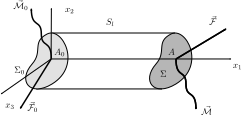
\includegraphics{../images/T1_Ch07-01}
    \end{center}
    \columnbreak
    On considère une poutre cylindrique de section $\Sigma$ et de longueur $l$
    \begin{equation*}
        \Omega = \left[ 0;l \right] \times \Sigma
    \end{equation*}
\end{multicols}
Les efforts de volume sont supposés nuls, $f_i= 0$ la surface latérale  $S_l= \left[ 0;l \right]\partial \Sigma$ est libre de contrainte
\begin{equation}
    \sigma_{ij} n_j = 0 \quad \left( x_2, x_3 \right) \in \partial \Sigma
    \label{eq:Ch07-001}
\end{equation}
et les efforts exercés sur les extrémités $\Sigma_0 \left( x_l =0 \right)$ et $\Sigma_1 \left( x_1 =l \right)$ sont caractérisés par leurs torseurs résultants $\left[ \mathcal{T}_0 \right]$ et $\left[ \mathcal{T}_1 \right]$.
Nous représenterons $\left[ \mathcal{T}_1 \right]$ par sa résultante $\vv{\mathcal{R}}$ et par son moment résultant $\vv{\mathcal{M}}$ au point $A\left( l,0,0 \right)$, centre de $\Sigma_1$, et de même $\left[ \mathcal{T}_0 \right]$ par sa résultante $\vv{\mathcal{R}}_0$ et par son moment résultant $\vv{\mathcal{M}}_0$ au point $A_0\left( l,0,0 \right)$, centre de $\Sigma_0$.
La poutre étant en équi1ibre, les efforts exerces sur et $\Sigma_0$ et $\Sigma_1$ doivent s'équilibrer, ce qui donne les relations vectorielles
\begin{equation}
    \left\{
    \begin{aligned}
        & \vv{\mathcal{R}}_0 + \vv{\mathcal{R}} = 0 \\
        & \vv{\mathcal{M}}_0 + \vv{\mathcal{M}} + \vv{A_0 A} \wedge  \vv{\mathcal{R}} = 0
    \end{aligned}
    \right.
    \label{eq:Ch07-002}
\end{equation}
Ainsi, on peut calculer $\vv{\mathcal{R}}_0$ et $\vv{\mathcal{M}}_0$ en fonction de $\vv{\mathcal{R}}$ et $\vv{\mathcal{M}}$, et les efforts exercés sur la poutre seront caractérisés par les deux vecteurs $\vv{\mathcal{R}}$ et $\vv{\mathcal{M}}$.

Pour relier ces efforts aux contraintes, il faut considérer les efforts exercés sur $\Omega$ à travers  $\Sigma_1$:
\begin{equation}
    \vv{n} = \left( 1,0,0 \right) \quad \vv{T} = \left( \sigma_{11}, \sigma_{12}, \sigma_{13} \right)
    \label{eq:Ch07-003}
\end{equation}
et intégrer sur toute la section.
Il vient
\begin{equation}
    \vv{\mathcal{R}} = \iint_{\Sigma_1} \vv{T} \ud S \quad,\quad \vv{\mathcal{M}} = \iint_{\Sigma_1} \vv{AM} \wedge \vv{T} \ud S
    \label{eq:Ch07-004}
\end{equation}
soit, en composantes
\begin{align}
    \mathcal{R}_1 &= \iint_{\Sigma_1} \sigma_{11} \ud x_2 \ud x_3    \label{eq:Ch07-005} \\
    \begin{split}
        \mathcal{R}_2 &= \iint_{\Sigma_1} \sigma_{12} \ud x_2 \ud x_3 \\
        \mathcal{R}_3 &= \iint_{\Sigma_1} \sigma_{13} \ud x_2 \ud x_3    \label{eq:Ch07-006}
    \end{split}
\end{align}
\begin{align}
    \mathcal{M}_1 &= \iint_{\Sigma_1} \left( x_2\sigma_{13} - x_3\sigma_{12} \right) \ud x_2 \ud x_3    \label{eq:Ch07-007} \\
    \begin{split}
        \mathcal{M}_2 &= \iint_{\Sigma_1} x_3\sigma_{11} \ud x_2 \ud x_3 \\
        \mathcal{M}_3 &= -\iint_{\Sigma_1} x_2\sigma_{11} \ud x_2 \ud x_3    \label{eq:Ch07-008}
    \end{split}
\end{align}

On aurait des formules analogues sur $\Sigma_0$.

Il est clair que le problème de Saint Venant ainsi posé n'est pas régulier, par manque de données.
En effet, les conditions \eqref{eq:Ch07-005},\eqref{eq:Ch07-006},\eqref{eq:Ch07-007},\eqref{eq:Ch07-008}, sont insuffisantes pour déterminer la répartition des efforts $\vv{T}$ sur $\Sigma_1$.
Pour obtenir un problème régulier, il faudrait préciser la manière dont les torseurs $\vv{T}$ sur $\Sigma_1$ sont appliqués.
Plus précisément, on peut imaginer plusieurs --	en fait une infinité -- répartitions d'efforts surfaciques vérifiant \eqref{eq:Ch07-005}, \eqref{eq:Ch07-006}, \eqref{eq:Ch07-007}, \eqref{eq:Ch07-008}, sur $\Sigma_1$, et de même sur $\Sigma_0$ chacune de ces répartitions sera associé un problème régulier (de type II), donc avec solution unique.
Ainsi le problème de Saint Venant, tel que nous l'avons formulé, admet une infinité de solutions.

\theoremstyle{definition}
\newtheorem*{psv}{Principe de Saint Venant}
\begin{psv}
    L'état de contrainte et de déformation loin des extrémités dépend uniquement du torseur des efforts appliqués, et non de la manière précise dont ces efforts sont appliqués.
\end{psv}

En d'autres termes, deux répartitions d'efforts surfaciques conduisant au même torseur, conduiront à deux solutions très voisines, sauf au voisinage immédiat des extrémités.
Ainsi le problème de Saint Venant admet une infinité de solutions, mais ces solutions sont très voisines les unes des autres, et il n'y a pas lieu de les distinguer -- à moins de vouloir des informations précises sur ce qui se passe au voisinage des extrémités.

Initialement, ce principe était d'origine intuitive; c'est lui qui se trouve à la base du célèbre mémoire de Saint Venant qui, déjà en 1856, contenait l'essentiel de ce chapitre.
Depuis, il a reçu de nombreuses vérifications expérimentales directes ou indirectes, car c'est le postulat de base de la Résistance des Matériaux.
Récemment, on a pu le démontrer dans certains cas particuliers par une étude mathématique des équations de l'élasticité.

Ce principe joue un rôle tout à fait essentiel pour deux raisons.
Tout d'abord, dans la pratique, on verra que l'on connaît assez rarement la répartition des efforts, alors que l'on a facilement leur torseur résultant.
Ensuite, c'est grâce à lui que nous pourrons résoudre le problème de Saint Venant, en jouant sur la latitude qui nous est laissée sur la répartition précise des efforts.
Notre démarche va être la suivante.
Nous allons tout d'abord décomposer le problème en 6 problèmes élémentaires correspondant à chacune des composantes de $\vv{\mathcal{R}}$ et $\vv{\mathcal{M}}$.
Ensuite, pour chacun de ces problèmes élémentaires, nous trouverons une solution, et par superposition, nous aurons une solution du problème complet.

Nous décomposons donc le problème de Saint Venant en 6 problèmes.
\paragraph{Problème 1:} Traction
\begin{equation}
    \mathcal{R}_1 = F, \quad \mathcal{R}_2 = \mathcal{R}_3 = 0, \quad \vv{\mathcal{M}} = 0
    \label{eq:Ch07-009}
\end{equation}
soit d'après \eqref{eq:Ch07-002}
\begin{multicols}{2}
    \begin{equation*}
        \vv{\mathcal{R}} = -\vv{\mathcal{R}}_0 = F \vv{e}_1, \quad \vv{\mathcal{M}} = \vv{\mathcal{M}}_0 = 0
    \end{equation*}
    \columnbreak
    \begin{center}
        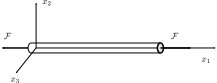
\includegraphics{../images/T1_Ch07-02}
    \end{center}
\end{multicols}
\paragraph{Problèmes 2 et 3:} Flexion composée
\begin{equation}
    \mathcal{R}_1 = 0 = \mathcal{R}_3, \quad \mathcal{R}_2 = F, \quad \vv{\mathcal{M}} = 0
    \label{eq:Ch07-010}
\end{equation}
pour le problème 2 (le problème 3 s'obtient en échangeant les indices 2 et 3), d'où
\begin{multicols}{2}
    \begin{equation*}
        \vv{\mathcal{R}} = -\vv{\mathcal{R}}_0 = F \vv{e}_2, \quad \vv{\mathcal{M}} = \vv{\mathcal{M}}_0 = -F l \vv{e}_3
    \end{equation*}
    \columnbreak
    \begin{center}
        \includegraphics{../images/T1_Ch07-03}
    \end{center}
\end{multicols}
\paragraph{Problème 4:} Torsion
\begin{equation}
    \vv{\mathcal{R}} = 0 , \quad \mathcal{M}_1 = \mathcal{M}, \quad \mathcal{M}_2 = \mathcal{M}_3 = 0
    \label{eq:Ch07-011}
\end{equation}
\begin{multicols}{2}
    \begin{equation*}
        \vv{\mathcal{R}} = \vv{\mathcal{R}}_0 = 0, \quad \vv{\mathcal{M}} = -\vv{\mathcal{M}}_0 = \mathcal{M} \vv{e}_1
    \end{equation*}
    \columnbreak
    \begin{center}
        \includegraphics{../images/T1_Ch07-04}
    \end{center}
\end{multicols}
\paragraph{Problèmes 5 et 6:} Flexion pure
\begin{equation}
    \vv{\mathcal{R}} = 0 , \quad \mathcal{M}_1 = \mathcal{M}_2 = 0, \quad \mathcal{M}_3 = 0
    \label{eq:Ch07-012}
\end{equation}
\begin{multicols}{2}
    \begin{equation*}
        \vv{\mathcal{R}} = \vv{\mathcal{R}}_0 = 0, \quad \vv{\mathcal{M}} = -\vv{\mathcal{M}}_0 = \mathcal{M} \vv{e}_3
    \end{equation*}
    \columnbreak
    \begin{center}
        \includegraphics{../images/T1_Ch07-05}
    \end{center}
\end{multicols}
pour le problème 6 (le problème 5 s'obtient en échangeant les indices 2 et 3).

Pour chacun de ces problèmes, les conditions portent sur les contraintes.
Nous adopterons donc l'approche du \ref{ssec:Ch06-1.4} en cherchant un champ de contraintes vérifiant
\begin{itemize}
    \item les équations d'équilibre avec $f_i=0$
    \item les équations de Beltrami
    \item les CL~\eqref{eq:Ch07-001} sur la surface latérale
    \item les conditions \eqref{eq:Ch07-005},\eqref{eq:Ch07-006},\eqref{eq:Ch07-007},\eqref{eq:Ch07-008}, pour le problème étudié.
\end{itemize}
\subsection{Répartition des contraintes normales} \label{ssec:Ch07-1.2}
On constate tout d'abord sur \eqref{eq:Ch07-005}, \eqref{eq:Ch07-006}, \eqref{eq:Ch07-007}, \eqref{eq:Ch07-008}, que $\mathcal{R}_1$, $\mathcal{M}_2$, $\mathcal{M}_3$ ne font intervenir que la contrainte normale (pour une facette de la section droite) $\sigma_{11}$.
Nous cherchons donc le champ des contraintes sous la forme
\begin{equation}
    \tens{\sigma} = 
    \begin{bmatrix}
        \sigma_{11}\left( x_1, x_2, x_3 \right) & 0 & 0 \\
        0 & 0 & 0 \\
        0 & 0 & 0
    \end{bmatrix}
    \label{eq:Ch07-013}
\end{equation}
Les CL \eqref{eq:Ch07-001} sur la surface latérale sont alors automatiquement vérifiées, puisque $\vv{n}=\left( 0,n_2,n_3 \right)$.
Les équations d'équilibre se réduisent à
\begin{equation}
    \frac{\partial \sigma_{11}}{\partial x_1} = 0 \quad,\quad \sigma_{11} = \sigma_{11}\left( x_2,x_3 \right)
    \label{eq:Ch07-014}
\end{equation}
Les équations de Beltrami \eqref{eq:Ch06-030} se réduisent alors à
\begin{equation}
    \frac{\partial^2 \sigma_{11}}{\partial x_2^2} = \frac{\partial^2 \sigma_{11}}{\partial x_3^2} = \frac{\partial^2 \sigma_{11}}{\partial x_2 \partial x_3} = 0
    \label{eq:Ch07-015}
\end{equation}
qui donne $\sigma_{11}$ fonction linéaire de $x_2$, $x_3$.
\begin{equation}
    \sigma_{11} = a + b x_2 + c x_3
    \label{eq:Ch07-016}
\end{equation}
Il ne reste plus à écrire que les conditions sur les extrémités, en reportant le tenseur des contraintes défini par \eqref{eq:Ch07-013} et \eqref{eq:Ch07-016} dans \eqref{eq:Ch07-005},\eqref{eq:Ch07-006},\eqref{eq:Ch07-007} et \eqref{eq:Ch07-008}, on obtient
\begin{equation}
    \left\{
    \begin{aligned}
        \mathcal{R}_1 &= a \iint_{\Sigma} \ud S + b \iint_{\Sigma} x_2 \ud S + c \iint_{\Sigma} x_3 \ud S \\
        -\mathcal{M}_3 &= a \iint_{\Sigma} x_2\ud S + b \iint_{\Sigma} x_2^2 \ud S + c \iint_{\Sigma} x_2 x_3 \ud S \\
        \mathcal{M}_2 &= a \iint_{\Sigma} x_3 \ud S + b \iint_{\Sigma} x_2 x_3 \ud S + c \iint_{\Sigma} x_3^2 \ud S \\
        \mathcal{R}_2 &= \mathcal{R}_3 = 0 \quad, \quad \mathcal{M}_1 = 0
    \end{aligned}
    \right.
    \label{eq:Ch07-017}
\end{equation}
Les intégrales qui interviennent dans \eqref{eq:Ch07-017} dépendent uniquement de la forme de la section.
Ainsi, le système \eqref{eq:Ch07-017} donnera $a$, $b$, $c$, en fonction de $\mathcal{R}_1$, $\mathcal{M}_2$ et $\mathcal{M}_3$.
Nous pourrons donc résoudre par un champ de contraintes de la forme \eqref{eq:Ch07-013}, \eqref{eq:Ch07-016}, les problèmes 1, 5 et 6 -- traction et flexion pure.

Pour déterminer complètement les contraintes, il reste à calculer $a$, $b$ et $c$, c'est à dire résoudre le système \eqref{eq:Ch07-017}.
Un choix judicieux du système d'axes $x_2x_3$ dans le plan de la section droite $\Sigma$ va faciliter cette résolution.
Tout d'abord, on choisit l'origine au centre de gravité de $\Sigma$, ce qui assure
\begin{equation}
    \iint_{\Sigma} x_2 \ud S = \iint_{\Sigma} x_3 \ud S = 0
    \label{eq:Ch07-018}
\end{equation}
Ensuite, on remarque que \eqref{eq:Ch07-017} fait intervenir les composantes du tenseur d'inertie de la section $\Sigma$
\begin{equation}
    J_{ij} = \iint_{\Sigma} x_i x_j \ud S \quad i,j = 2,3
    \label{eq:Ch07-019}
\end{equation}
c'est un tenseur plan symétrique, donc diagonalisable.
On peut trouver dans le plan $x_2$, $x_3$ deux directions principales d'inertie perpendiculaires telles que le moment produit $J_{23}$ soit nul
\begin{equation}
    J_{23} = \iint_{\Sigma} x_2 x_3 \ud S = 0
    \label{eq:Ch07-020}
\end{equation}
Nous choisirons ces directions principales comme axes $x_2$, $x_3$.
Pratiquement, si la section a un axe de symétrie, alors cet axe est principal d'inertie, car la symétrie entraîne \eqref{eq:Ch07-02O}.
Sinon la diagonalisation est facile, et on peut en particulier utiliser la méthode géométrique exposée au paragraphe~\ref{ssec:Ch03-3.2} pour le tenseur des contraintes.

Avec ce choix d'axes, \eqref{eq:Ch07-017} devient simplement
\begin{equation}
    \mathcal{R}_1 = a S, \quad -\mathcal{M}_3 = b J_2, \quad \mathcal{M}_2 = c J_3, \quad J_2 = \iint_{\Sigma} x_2^2 \ud S, \quad J_3 = \iint_{\Sigma} x_3^2 \ud S
    \label{eq:Ch07-021}
\end{equation}
où $S$ est la surface de $\Sigma$ et $J_2$, $J_3$ les moments d'inertie principaux.
On obtient donc pour $\sigma_{11}$
\begin{equation}
    \sigma_{11} = \frac{\mathcal{R}_1}{S} - \frac{\mathcal{M}_3}{J_2} x_2 + \frac{\mathcal{M}_2}{J_3}x_3
    \label{eq:Ch07-022}
\end{equation}
et on a trouvé un champ de contraintes convenables pour les problèmes 1, 5 et 6.

En particulier, pour la traction -- Problème 1 -- on retrouve la solution présenté au paragraphe~\ref{ssec:Ch04-1.4}
\begin{equation}
    \tens{\sigma} = 
    \begin{bmatrix}
        \frac{F}{S} & 0 & 0 \\
        0 & 0 & 0 \\
        0 & 0 & 0
    \end{bmatrix}
    \quad
    \begin{cases}
        u_1 = \frac{F}{ES} x_1 \\
        u_2 = -\nu \frac{F}{ES} x_2 \\
        u_3 = -\nu \frac{F}{ES}  x_3
    \end{cases}
    \label{eq:Ch07-023}
\end{equation}
C'est la solution du problème régulier associé aux CL
\begin{equation}
    x_1 = 0 \text{ et } x_1 = l: \quad \sigma_{11} = F/S, \ \sigma_{12} = \sigma_{13} = 0
    \label{eq:Ch07-024}
\end{equation}
En général, les CL réelles -- par exemple dans un essai de traction -- sont différentes, mais le principe de Saint Venant nous assure que cela n'a guère d'importance, à condition de se placer loin des têtes d'amarrage, et c'est bien ce que l'on fait dans un essal de traction.

\subsection{Flexion pure} \label{ssec:Ch07-1.3}
Considérons maintenant le problème 6 -- le problème 5 se traiterait de manière identique.
Le tenseur des contraintes a la forme suivante
\begin{equation}
    \tens{\sigma} = 
    \begin{bmatrix}
        -\frac{\mathcal{M}}{J}x_2 & 0 & 0 \\
        0 & 0 & 0 \\
        0 & 0 & 0
    \end{bmatrix}
    \label{eq:Ch07-025}
\end{equation}
où l'on a supprimé l'indice $2$ sur $J$
\begin{equation}
    J=J_2 = \iint_{\Sigma} x_2^2 \ud S
    \label{eq:Ch07-026}
\end{equation}
Il reste à calculer les déplacements.
Comme au paragraphe~\ref{ssec:Ch06-2.1}, nous procéderons directement en écrivant le tenseur des déformations
\begin{equation}
    \tens{\varepsilon} = 
    \begin{bmatrix}
        -\frac{\mathcal{M}}{EJ}x_2 & 0 & 0 \\
        0 & \nu\frac{\mathcal{M}}{EJ}x_2 & 0 \\
        0 & 0 & \nu\frac{\mathcal{M}}{EJ}x_2
    \end{bmatrix}
    \label{eq:Ch07-027}
\end{equation}
\begin{equation}
    \left\{
    \begin{aligned}
        \varepsilon_{11} = \frac{\partial u_1}{\partial x_1} = -\frac{\mathcal{M}}{EJ}x_2 & \Rightarrow u_1 = \frac{\mathcal{M}}{EJ}x_1x_2 + \varphi_1 \left( x_2,x_3 \right) \\
        \varepsilon_{22} = \frac{\partial u_2}{\partial x_2} = \frac{\nu\mathcal{M}}{EJ}x_2 & \Rightarrow u_2 = \frac{\nu\mathcal{M}}{EJ}x_2^2 + \varphi_2 \left( x_1,x_3 \right) \\
        \varepsilon_{33} = \frac{\partial u_3}{\partial x_3} = \frac{\nu\mathcal{M}}{EJ}x_2 & \Rightarrow u_3 = \frac{\nu\mathcal{M}}{EJ}x_2x_3 + \varphi_3 \left( x_1,x_2 \right)
    \end{aligned}
    \right.
    \label{eq:Ch07-028}
\end{equation}
\begin{equation}
    \left\{
    \begin{aligned}
        2 \varepsilon_{12} &= \frac{\partial u_1}{\partial x_2} + \frac{\partial u_2}{\partial x_1} = - \frac{\mathcal{M}}{EJ}x_1 + \varphi_{1,2} + \varphi_{2,1} = 0 \\
        2 \varepsilon_{23} &= \frac{\partial u_2}{\partial x_3} + \frac{\partial u_3}{\partial x_2} = \frac{\nu\mathcal{M}}{EJ}x_3 + \varphi_{2,3} + \varphi_{3,2} = 0 \\
        2 \varepsilon_{31} &= \frac{\partial u_3}{\partial x_1} + \frac{\partial u_1}{\partial x_3} = \varphi_{1,3} + \varphi_{3,1} = 0
    \end{aligned}
    \right.
    \label{eq:Ch07-029}
\end{equation}
et on obtient la solution particulière 
\begin{equation}
    \varphi_1 = \varphi_3 = 0 \quad , \quad \varphi_2 = \frac{\mathcal{M}}{2EJ} \left( x_1^2 - \nu x_3^2 \right)
    \label{eq:Ch07-030}
\end{equation}
Le déplacement est donc donne par
\begin{equation}
    \left\{
    \begin{aligned}
        u_1 & = -\frac{\mathcal{M}}{EJ} x_1x_2 -\omega_3^0x_2 \\
        u_2 & = \frac{\mathcal{M}}{2EJ} \left[ x_1^2 + \nu \left( x_2^2 - x_3^2 \right) \right] +\omega_3^0x_1 +u_2^0 \\
        u_3 & = \frac{\nu\mathcal{M}}{EJ} x_2x_3
    \end{aligned}
    \right.
    \label{eq:Ch07-031}
\end{equation}
où, en vue des applications futures, nous n'avons conservé qu'une partie du déplacement de solide.

La déformation de la ligne moyenne est donnée par
\begin{equation}
    u_1 = u_3 = 0 \quad , \quad u_2 = \frac{\mathcal{M}}{2EJ}x_1^2 + \omega_3^0 x_1 = v(x_1)
    \label{eq:Ch07-032}
\end{equation}
tandis que la déformée d'une section droite $x_1=x_1^0$ est caractérisée par
\begin{equation}
    u_1 = - \left( \frac{\mathcal{M}}{EJ}x_1^0 + \omega_3^0 \right) x_2 = - \left.\frac{\ud v}{\ud x_1}\right|_{x_1^0} x_2
    \label{eq:Ch07-033}
\end{equation}
Les relations \eqref{eq:Ch07-032} et \eqref{eq:Ch07-033} montrent qu'après la déformation la ligne moyenne devient une parabole et que les sections droites restent planes et perpendiculaires à la ligne moyenne
\begin{center}
    \includegraphics{../images/T1_Ch07-06}
\end{center}

On construit souvent la théorie élémentaire de la flexion à partir de
\paragraph{Hypothèse de Navier-Bernoulli.} Les sections droites restent planes et normales à la fibre moyenne.

Cette hypothèse se trouve donc vérifiée ici.
On constate également que le moment $\mathcal{M}$ appliqué produit une courbure de la ligne moyenne
\begin{equation}
    \Xi = \frac{\ud^2 v}{\ud x_1} \frac{\mathcal{M}}{EJ}
    \label{eq:Ch07-034}
\end{equation}
Ainsi, on pourrait envisager de mesurer le module d'Young $E$ d'un matériau élastique par un essai de flexion: on impose un moment de flexion $\mathcal{M}$ et on observe la courbure $\Xi$, ce qui détermine la «~rigidité~» de la poutre $EJ$ produit d'une rigidité matérielle $E$, liée au matériau, et d'une rigidité géométrique $J$, donnée par \eqref{eq:Ch07-026} et liée à la géométrie de la section droite $\Sigma$.

En chaque point, on a un état de contraintes de traction simple, et le critère de limite d'élasticité donnera 
\begin{equation}
    \left|\sigma_{11}\right| = \frac{\mathcal{M}}{J} \left|x_2\right| < \sigma_e
    \label{eq:Ch07-035}
\end{equation}
soit, en introduisant $\eta$ valeur maximale de $\left|x_2\right|$
\begin{equation}
    \frac{\mathcal{M}}{J/\eta} < \sigma_e \quad , \quad \eta = \left|x_2\right|_{max}
    \label{eq:Ch07-036}
\end{equation}
Ainsi, d'un point de vue géométrique, la rigidité d'une poutre est caractérisée  par le moment  d'inertie $J$,  tandis que sa résistance est caractérisée par le rapport $J/\eta$

\underline{Section rectangulaire}
\begin{multicols}{2}
    \begin{center}
        \includegraphics{../images/T1_Ch07-07}
    \end{center}
    \columnbreak
    \begin{displaymath}
        J = \frac{bh^3}{12},\ \frac{J}{\eta} = \frac{bh^2}{6},\ \frac{J}{S} = \frac{h^2}{12},\ \frac{J}{\eta S} = \frac{h}{6}
    \end{displaymath}
\end{multicols}
\underline{Section en I}
\begin{multicols}{2}
    \begin{center}
        \includegraphics{../images/T1_Ch07-08}
    \end{center}
    \columnbreak
    \begin{displaymath}
        J \approx \frac{bh^2l}{2},\ \frac{J}{\eta} \approx bhl,\ \frac{J}{S} = \frac{h^2}{4},\ \frac{J}{\eta S} = \frac{h}{2}
    \end{displaymath}
\end{multicols}
Ceci montre la supériorité, à poids égal,de la section en $I$ sur la section rectangulaire et, plus généralement, des sections en profil mince sur les sections massives.

\section{Torsion} \label{sec:Ch07-2}
\subsection{Section circulaire ou annulaire} \label{ssec:Ch07-2.1}
Avant d'aborder le cas général, nous allons envisager le cas simple d'une section circulaire ou annulaire.
On ohserve alors qu'en torsion, chaque section droite tourne, par rapport à la section $x_1=O$, d'un angle proportionnel à la distance
\begin{multicols}{2}
    \begin{center}
        \includegraphics{../images/T1_Ch07-09}
    \end{center}
    \begin{center}
        \includegraphics{../images/T1_Ch07-10}
    \end{center}
\end{multicols}
Nous postulons donc un champ de déplacements
\begin{equation}
    u_1 = 0 \quad,\quad u_2 = -\alpha x_1 x_3 \quad,\quad u_3 = \alpha x_1 x_2
    \label{eq:Ch07-037}
\end{equation}
On obtient alors pour le gradient du déplacement et pour le tenseur des déformations
\begin{equation}
    u_{i,j} = 
    \begin{bmatrix}
        0 & 0 & 0 \\
        -\alpha x_3 & 0 & -\alpha x_1 \\
        \alpha x_2 & \alpha x_1 & 0
    \end{bmatrix}
    \varepsilon_{i,j} = 
    \begin{bmatrix}
        0 & \frac{\alpha}{2}x_3 & \frac{\alpha}{2}x_2 \\
        -\frac{\alpha}{2}x_3 & 0 & 0 \\
        \frac{\alpha}{2}x_2 & 0 & 0
    \end{bmatrix}
    \label{eq:Ch07-038}
\end{equation}
La loi de comportement donne alors le tenseur des contraintes
\begin{equation}
    \sigma_{i,j} = 
    \begin{bmatrix}
        0 & -G\alpha x_2 & G\alpha x_2 \\
        -G \alpha x_3 & 0 & 0 \\
        G \alpha x_2 & 0 & 0
    \end{bmatrix}
    \label{eq:Ch07-039}
\end{equation}
Ce champ de contraintes vérifie directement
\begin{itemize}
    \item les équations d'équilibre,
    \item les conditions aux limites sur la surface latérale $\vec{n} = \pm \left( x_1/r, x_2/r, 0 \right)$
\end{itemize}
Il n'est pas nécessaire de vérifier les équations de  Beltrami,  puisque l'on est parti d'un champ de déplacements.
Il ne reste donc plus qu'à écrire le torseur des efforts appliqués sur $\Sigma_1$.
Puisque $\sigma_{11}$ est nul, $\mathcal{M}_2$ et $\mathcal{M}_3$ sont nuls.
Par symétrie, $\mathcal{R}_2$ et $\mathcal{R}_3$, sont nuls, et il reste simplement
\begin{equation}
    \mathcal{M}_1 = \iint_{\Sigma} G \alpha \left( x_2^2 + x_3^2 \right) \ud S = G\alpha \iint_{\Sigma} r^2 \ud S    
    \label{eq:Ch07-040} 
\end{equation}
On a donc résolu le problème 4 avec
\begin{equation}
    \mathcal{M} = G I_0 \alpha \quad,\quad I_0 = \iint_{\Sigma} r^2 \ud S
    \label{eq:Ch07-041}
\end{equation}
Le moment de torsion $\mathcal{M}$ crée un «~angle unitaire de torsion~» $\alpha$, et le module de rigidité $G I_0$ est à nouveau le produit d'une rigidité matérielle $G=\mu$ et d'une rigidité géométrique $I_0$ moment d'inertie polaire de la section.

Le vecteur contrainte associé à la section droite est
\begin{equation}
    \vec{T} = \left( 0, -G\alpha x_3, G \alpha x_2 \right)
    \label{eq:Ch07-042}
\end{equation}
\begin{multicols}{2}
    \begin{center}
        \includegraphics{../images/T1_Ch07-11}
    \end{center}
    \columnbreak
    On a uniquement une contrainte de cisaillement perpendiculaire au rayon et de module $G\alpha r$.
    En notant $\vec{e}_r$, $\vec{e}_{\theta}$, les vecteurs de base associés aux coordonnées polaires $r$, $\theta$ dans le plan $x_2,x_3$ on a
\end{multicols}
\begin{equation}
    \vec{T} = G \alpha r \vec{e}_{\theta} 
    \label{eq:Ch07-043}
\end{equation}
et dans le repère $\vec{e}_r$, $\vec{e}_{\theta}$, $\vec{e}_{1}$ associé aux coordonnées cylindriques autour de $x_1$, le tenseur des contraintes a pour composantes
\begin{equation}
    \tens{\sigma} = 
    \begin{bmatrix}
        0 & 0 & 0\\
        0 & 0 & G\alpha r\\
        0 & G\alpha r & 0
    \end{bmatrix}
    \label{eq:Ch07-044}
\end{equation}
L'état de contraintes en chaque point est un état de cisaillement simple, et le critère de limite d'élasticité s'écrit
\begin{equation}
    |\vec{T}| = G \alpha r < \tau_e    
    \label{eq:Ch07-045} 
\end{equation}
où $\tau_e$ est la limite élastique en cisaillement simple donnée par \eqref{eq:Ch05-071}.
En introduisant $R$ rayon de la section, il vient, en combinant avec \eqref{eq:Ch07-041},
\begin{equation}
    \frac{\mathcal{M}}{I_0/\mathcal{R}} < \tau_e    
    \label{eq:Ch07-046} 
\end{equation}

La rigidité à la torsion d'un arbre circulaire ou annulaire est donc caractérisée par le moment d'inertie polaire de sa section $I_0$ et sa résistance par le rapport $I_0/\mathcal{R}$.

\underline{Section circulaire}
\begin{multicols}{2}
    \begin{center}
        \includegraphics{../images/T1_Ch07-12}
    \end{center}
    \columnbreak
    \begin{displaymath}
        I_0 = \frac{\pi D^4}{32},\ \frac{I_0}{S} = \frac{D^2}{8},\ \frac{I_0}{\mathcal{R}} = \frac{\pi D^3}{16},\ \frac{I_0}{\mathcal{R} S} = \frac{D}{4}
    \end{displaymath}
\end{multicols}
\underline{Section en tube mince}
\begin{multicols}{2}
    \begin{center}
        \includegraphics{../images/T1_Ch07-13}
    \end{center}
    \columnbreak
    \begin{displaymath}
        I_0 = \frac{r\pi D^3 e}{4},\ \frac{I_0}{S} = \frac{D^2}{4},\ \frac{I_0}{\mathcal{R}} = \frac{\pi D^3 e}{2},\ \frac{I_0}{\mathcal{R} S} = \frac{D}{2}
    \end{displaymath}
\end{multicols}
Ces relations montrent la supériorité, à poids égal, des sections annulaires sur les sections massives.
Dans le cas des tubes minces, on constate aussi que $r \sim D/2$ et que les composantes \eqref{eq:Ch07-044} du tenseur des contraintes dans le repère $\left( \vec{e}_r, \vec{e}_{\theta}, \vec{e}_1 \right)$ peuvent s'écrire
\begin{displaymath}
    \tens{\sigma} \sim
    \begin{bmatrix}
        0 & 0 & 0 \\
        0 & 0 & G \alpha \frac{D}{2} \\
        0 & G\alpha \frac{D}{2} & 0
    \end{bmatrix}
\end{displaymath}
soit, compte tenu de \eqref{eq:Ch07-041} et de la valeur de $I_0$
\begin{equation}
    \tens{\sigma} \sim
    \begin{bmatrix}
        0 & 0 & 0 \\
        0 & 0 & \frac{2\mathcal{M}}{\pi D^2 e} \\
        0 & \frac{2\mathcal{M}}{\pi D^2 e} & 0
    \end{bmatrix}
    \label{eq:Ch07-047}
\end{equation}
ce qui, superposé à l'état de contraintes dû à une traction simple, redonne bien la forme \eqref{eq:Ch04-036} obtenue au paragraphe~\ref{ssec:Ch04-1.4}.
\subsection{Théorie générale} \label{ssec:Ch07-2.2}
Nous considérons maintenant le problème 4 dans le cas d'une section quelConque.
Le paragraphe~\ref{sec:Ch07-1} a montré que la contrainte normale $\sigma_{11}$ était déterminée par $\mathcal{R}_1$, $\mathcal{M}_2$, $\mathcal{M}_3$.
Puisqu'ici ils sont nuls, on prendra donc $\sigma_{11}=0$.
Les contraintes de cisaillement $\sigma_{12}$ et $\sigma_{13}$ par contre ne peuvent pas être nulles d'après \eqref{eq:Ch07-007}.
Nous cherchons donc un champ de contraintes sous la forme
\begin{equation}
    \tens{\sigma} = 
    \begin{bmatrix}
        0 & \sigma_{12} & \sigma_{13} \\
        \sigma_{12} & 0 & 0\\
        \sigma_{13} & 0 & 0
    \end{bmatrix}
    \label{eq:Ch07-048}
\end{equation}
avec $\sigma_{12}$ et $\sigma_{13}$ fonctions de $\left( x_1, x_2, x_3 \right)$.
Les équations d'équilibre donnent
\begin{equation}
    \frac{\partial \sigma_{12}}{\partial x_2} + \frac{\partial \sigma_{13}}{\partial x_3} = 0
    \label{eq:Ch07-049}
\end{equation}
\begin{equation}
    \begin{cases}
        \frac{\partial \sigma_{12}}{\partial x_1} = 0 & \Rightarrow \quad \sigma_{12} = \sigma_{12} \left( x_2, x_3 \right) \\
        \frac{\partial \sigma_{13}}{\partial x_1} = 0 & \Rightarrow \quad \sigma_{13} = \sigma_{13} \left( x_2, x_3 \right)
    \end{cases}
    \label{eq:Ch07-050}
\end{equation}
L'équation \eqref{eq:Ch07-049} montre alors -- voir par exemple le Lemme 2 du paragraphe~\ref{ssec:Ch03-3.1} -- que la forme différentielle
\begin{equation}
    \ud \Phi = \sigma_{12} \ud x_3 - \sigma_{13} \ud x_2
    \label{eq:Ch07-051}
\end{equation}
est intégrable, c'est à dire il existe une «~fonction des contraintes~» $\Phi\left( x_2, x_3 \right)$ telle que
\begin{equation}
    \sigma_{12} = \frac{\partial \Phi}{\partial x_3} \quad , \quad \sigma_{13} = - \frac{\partial \Phi}{\partial x_2}
    \label{eq:Ch07-052}
\end{equation}
Les équations de Beltrami donnent alors
\begin{equation}
    \frac{\partial}{\partial x_2} \Delta \Phi = \frac{\partial}{\partial x_3} \Delta \Phi = 0
    \label{eq:Ch07-053}
\end{equation}
ce qui montre que est constant; nous noterons $-2G\alpha$ cette constante, $\alpha$ étant une constante d'intégration dont nous verrons plus loin la signification
\begin{equation}
    \Delta \Phi + 2 G \alpha = 0
    \label{eq:Ch07-054}
\end{equation}
La CL \eqref{eq:Ch07-001} sur la surface latérale s'écrit
\begin{equation}
    \sigma_{12} n_2 + \sigma_{13} n_3 = 0
    \label{eq:Ch07-055}
\end{equation}
\begin{multicols}{2}
    \begin{center}
        \includegraphics{../images/T1_Ch07-14}
    \end{center}
    \columnbreak
    En introduisant le vecteur unitaire tangent à $\partial \Sigma$
    \begin{displaymath}
        \vec{t} = \left( \ud x_2 / \ud s, \ud x_3/\ud s \right)
    \end{displaymath}
    il vient
\end{multicols}
\begin{equation}
    n_2 = t_3 = \frac{\ud x_3}{\ud s} \quad , \quad n_3 = -t_2 = - \frac{\ud x_2}{\ud s}
    \label{eq:Ch07-056}
\end{equation}
de sorte que, compte tenu de \eqref{eq:Ch07-052}, la CL \eqref{eq:Ch07-055} devient
\begin{equation}
    \frac{\partial \Phi}{\partial x_3} \frac{\ud x_3}{\ud s} + \frac{\partial \Phi}{\partial x_2} \frac{\ud x_2}{\ud s} = \frac{\ud \Phi}{\ud s}
    \label{eq:Ch07-057}
\end{equation}
La fonction $\Phi\left( x_2, x_3 \right)$ reste constante lorsque l'on suit $\partial \Sigma$, donc sur chaque composante connexe de $\partial \Sigma$.
Nous supposerons désormais que la section $\Sigma$ est simplement connexe.
On tire alors de \eqref{eq:Ch07-057} que $\Phi$ est constant sur $\partial \Sigma$ et on peut toujours choisir cette constante nulle
\begin{equation}
    \Phi_{|_{\partial \Sigma}} = 0
    \label{eq:Ch07-058}
\end{equation}
La fonction de contrainte $\Phi$ est donc déterminée par \eqref{eq:Ch07-054} et \eqref{eq:Ch07-055}, équations qui définissent «~problème de Dirichlet~», qui admet donc une solution unique.
Par le changement de fonction
\begin{equation}
    \Phi \left( x_2, x_3 \right) = G \alpha \varphi \left( x_2, x_3 \right)
    \label{eq:Ch07-059}
\end{equation}
ce problème se transforme en
\begin{equation}
    \left\{
    \begin{aligned}
        & \Delta \varphi + 2 = 0 \\
        & \varphi_{|_{\partial \Sigma}} = 0
    \end{aligned}
    \right.
    \label{eq:Ch07-060}
\end{equation}
et la fonction $\varphi$ unique solution du problème \eqref{eq:Ch07-060}, dépend uniquement de la forme de la section $\Sigma$.

Il ne reste plus qu'à déterminer la constante $\alpha$, ce que nous allons faire en calculant les efforts exercés sur $\Sigma_1$.
On sait déjà que $\mathcal{R}_1 = \mathcal{M}_2 = \mathcal{M}_3 = 0$.
Pour calculer les autres composantes, nous utiliserons la formule de Stokes
\begin{equation}
    \iint_{S} \left( \frac{\partial Q}{\partial x_2} - \frac{\partial P}{\partial x_3} \right) \ud x_2 \ud x_3 = \oint_{\partial S} P \ud x_2 + Q \ud x_3
    \label{eq:Ch07-061}
\end{equation}
A partir de \eqref{eq:Ch07-006} et \eqref{eq:Ch07-052}, il vient
\begin{equation}
    \mathcal{R}_2 = \iint_{\Sigma} \sigma_{12} \ud x_2 \ud x_3 = \iint_{\Sigma} \frac{\partial \Phi}{\partial x_3} \ud x_2 \ud x_3 = - \oint_{\partial \Sigma} \Phi \ud x_2 = 0
    \label{eq:Ch07-062}
\end{equation}
d'après la formule de Stokes \eqref{eq:Ch07-061} et \eqref{eq:Ch07-058}.
De la même manière, on a $\mathcal{R}_3 = 0$.
A partir de \eqref{eq:Ch07-007} on a
\begin{equation}
    \begin{aligned}
        \mathcal{M}_1 &= -\iint_{\Sigma} \left( x_2 \frac{\partial \Phi}{\partial x_2} + x_3 \frac{\partial \Phi}{\partial x_3} \right) \ud x_2 \ud x_3 \\
        &= -\iint_{\Sigma} \left[ \frac{\partial}{\partial x_2} \left( x_2 \Phi \right) + \frac{\partial}{\partial x_3} \left( x_3 \Phi \right) - 2\Phi \right] \ud x_2 \ud x_3 \\
        &= 2 \iint_{\Sigma} \Phi \ud x_2 \ud x_3 + \cancel{\oint_{\partial \Sigma} x_3 \Phi \ud x_2} - \cancel{x_2 \Phi \ud x_3} \\
        &= 2 G \alpha \iint_{\Sigma} \varphi \ud x_2 \ud x_3
    \end{aligned}
    \label{eq:Ch07-063}
\end{equation}
Finalement, le champ de contraintes construit permet de résoudre le problème 4 avec
\begin{equation}
    \alpha = \frac{\mathcal{M}}{GI} \quad,\quad I = 2 \iint_{\Sigma} \varphi \ud x_2 \ud x_3
    \label{eq:Ch07-064} 
\end{equation}
La constante $I$ est appelée «~module de rigidité~» de la section $\Sigma$, et, comme $\varphi$ elle ne dépend que de la forme de $\Sigma$.

En chaque point de la section, l'état de contraintes est un état de cisaillement simple caractérisé par le vecteur contrainte $\vec{T}$ associé à la section droite
\begin{equation}
    \vec{T} = \left( O, \sigma_{12}, \sigma_{13} \right)
    \label{eq:Ch07-065} 
\end{equation}
La CL~\eqref{eq:Ch07-001} exprime que, sur la frontière $\partial \Sigma$, $\vec{T}$ est tangent à $\partial \Sigma$ 
\begin{equation}
    \text{sur } \partial \Sigma \quad \vec{T} \cdot \vec{n} = 0    
    \label{eq:Ch07-066}
\end{equation}
\begin{multicols}{2}
    Les relations \eqref{eq:Ch07-012} montrent que les courbes $\Phi = \text{Cte}$ sont les enveloppes du champ de vecteurs $\vec{T}$.
    \columnbreak
    \begin{center}
        \includegraphics{../images/T1_Ch07-15}
    \end{center}
\end{multicols}

L'état de contraintes étant un état de cisaillement simple, le critère de limite d'élasticité donne 
\begin{equation}
    \abs{\vec{T}} = \sqrt{\sigma_{12}^2 + \sigma_{13}^2} < \tau_e    
    \label{eq:Ch07-067}
\end{equation}
avec $\tau_e$ donné par \eqref{eq:Ch05-071}.
A partir de $\Phi$ ou $\varphi$ cette condition donne 
\[
\sqrt{\Phi_{,3}^2 + \Phi_{,2}^2} = G \alpha \sqrt{\varphi_{,3}^2 + \varphi_{,2}^2} = G \alpha \abs{\grad \varphi} < \tau_e
\]
Soit finalement
\begin{equation}
    \frac{\mathcal{M}}{I/\rho} < \tau_e \quad , \quad \rho = \left[ \sup_{\Sigma} \abs{\grad \varphi} \right]^{-1}
    \label{eq:Ch07-068}
\end{equation}
où $\rho$ est une longueur caractéristique de la section $\Sigma$.
On peut par ailleurs montrer que la borne supérieure de $\abs{\grad \varphi}$ est nécessairement atteinte sur la frontière de $\Sigma$.
Ainsi le problème général de la torsion est résolu, sitôt que l'on connaît la solution $\varphi\left( x_2,x_3 \right)$ du problème \eqref{eq:Ch07-060}. 

\subsection{Calcul du déplacehent} \label{ssec:Ch07-2.3}
Pour terminer le calcul, il reste à calculer le déplacement.
A partir de \eqref{eq:Ch07-048}, \eqref{eq:Ch07-052} et \eqref{eq:Ch07-059}, le tenseur des déformations est donné par
\begin{equation}
    \tens{\varepsilon} = 
    \frac{\alpha}{2} 
    \begin{bmatrix}
        0 & \varphi_{,3} & -\varphi_{,2} \\
        \varphi_{,3} & 0 & 0 \\
        -\varphi_{,2} & 0 & 0
    \end{bmatrix}
    \label{eq:Ch07-069}
\end{equation}
et on peut intégrer le champ de déplacements
\begin{equation}
    \left\{
    \begin{aligned}
        \varepsilon_{11} = u_{1,1} = 0 & \Rightarrow & u_1 =u_1 \left( x_2,x_3 \right) \\
        \varepsilon_{22} = u_{2,2} = 0 & \Rightarrow & u_2 =u_2 \left( x_1,x_3 \right) \\
        \varepsilon_{33} = u_{3,3} = 0 & \Rightarrow & u_3 =u_3 \left( x_1,x_2 \right)
    \end{aligned}
    \right.
    \label{eq:Ch07-070}
\end{equation}
\[
2\varepsilon_{23} = u_{2,3} + u_{3,2} =0 \quad \Rightarrow \quad u_{2,3} = - u_{3,2} = A(x_1)
\]
(car $u_{2,3} = u_{2,3}(x_1,x_3)$ et $u_{3,2} = u_{3,2} (x_1,x_2)$) et on a
\begin{equation}
    \left\{
    \begin{aligned}
        u_2 = A(x_1) x_3 + B(x_1)\\
        u_3 = -A(x_1) x_2 + C(x_1)
    \end{aligned}
    \right.
    \label{eq:Ch07-071} 
\end{equation}
et on peut interpréter $A(x_1)$ comme étant la rotation de la section droite d'abscisse $x_1$
\begin{equation}
    \left\{
    \begin{aligned}
        &2\varepsilon_{12} = u_{1,2} + u_{2,1} = u_{1,2} + A'(x_1) x_3 + B'(x_1) = \alpha \varphi_{,3}\\
        &2\varepsilon_{13} = u_{1,3} + u_{3,1} = u_{1,3} - A'(x_1) x_2 + C'(x_1) = \alpha \varphi_{,2}
    \end{aligned}
    \right.
    \label{eq:Ch07-072}
\end{equation}
Mais dans ces relations, seules les dérivées $A'(x_1) (=\ud A /\ud x_1)$, $B'(x_1)$ et dépendent de $C'(x_1)$ elles doivent donc être constantes 
\[
A(x_1) = -a x_1 +d \quad,\quad B(x_1) = b x_1 +e \quad,\quad C(x_1) = c x_1 +f
\]
\begin{equation}
    \left\{
    \begin{aligned}
        u_2 &= -a x_1 x_3 + \ud x_3 + b x_1 + e\\
        u_3 &= a x_1 x_2 \underbrace{- \ud x_3 + c x_1 + f}_{\text{Déplacement de solide rigide}}
    \end{aligned}
    \right.
    \label{eq:Ch07-073} 
\end{equation}
On voit sur \eqref{eq:Ch07-073} que les 5 constantes $b$, $c$, $d$, $e$, $f$ correspondent au déplacement de solide rigide arbitraire, qui doit nécessairement s'introduire dans l'intégration.
A un déplacement de solide près, on a donc 
\begin{equation}
    u_2 = -a x_1 x_3 \quad , \quad u_3 = a x_1 x_2
    \label{eq:Ch07-074}
\end{equation}
ce qui correspond, comme dans le cas de la section circulaire, à une rotation de chaque section d'un angle proportionnel à la distance à l'origine; la constante $a$, rotation par unité de longueur, est donc «~l'angle unitaire de torsion~» introduit au paragraphe~\ref{ssec:Ch07-1.1} pour la section circulaire.
On peut maintenant calculer $u_1$ à partir de \eqref{eq:Ch07-072} 
\begin{equation}
    u_{1,2} = \alpha \varphi_{,3} + a x_3 \quad , \quad u_{1,3} = -\alpha \varphi_{,2} - a x_2
    \label{eq:Ch07-075}
\end{equation}
système qui sera intégrable si et seulement si $u_{1,23} = u_{1,32}$
\begin{displaymath}
    \alpha \Delta \varphi + 2 a = 0
\end{displaymath}
ce qui, d'après \eqref{eq:Ch07-060}, donne finalement $a=\alpha$, et la constante $\alpha$, introduite en \eqref{eq:Ch07-054} est l'angle unitaire de torsion, et le déplacement est finalement, à un déplacement de solide près 
\begin{equation}
    \left\{
    \begin{aligned}
        u_1 &= \alpha \psi (x_2, x_3) \\
        u_2 &= - \alpha x_1 x_3 \\
        u_3 &= \alpha x_1 x_2
    \end{aligned}
    \right.
    \label{eq:Ch07-076}
\end{equation}
Ainsi, la rotation de chaque section s'accompagne d'un «~gauchissement~» que l'on peut observer expérimentalement.
La fonction de gauchissement $\psi$ est donnée par 
\begin{equation}
    \frac{\partial \Psi}{\partial x_2} = \left( \frac{\partial \varphi}{\partial x_3} + x_3 \right) \quad , \quad \frac{\partial \Psi}{\partial x_3} = -\left( \frac{\partial \varphi}{\partial x_2} + x_2 \right)
    \label{eq:Ch07-077}
\end{equation}
et $\psi$ est la fonction harmonique conjuguée de la fonction harmonique $\varphi + \frac{1}{2} (x_2^2 + x_3^2)$.
Si 	on calcule sur $\partial \Sigma$ la dérivée normale de $\psi$, il vient, en utilisant \eqref{eq:Ch07-056} et \eqref{eq:Ch07-057} 
\begin{align*}
    \frac{\ud \psi}{\ud n} &= \frac{\partial \psi}{\partial x_2} n_2 + \frac{\partial \psi}{\partial x_3} n_3 \\
    &= \left( \frac{\partial \varphi}{\partial x_3} \frac{\ud x_2}{\ud s} + \frac{\partial \varphi}{\partial x_2} \frac{\ud x_2}{\ud s} \right) + x_3 \frac{\ud x_2}{\ud s} + x_2 \frac{\ud x_2}{\ud s} \\
    &= \frac{\ud}{\ud s} \left[ \frac{1}{2} \left( x_2^2 + x_3^2 \right) \right]
\end{align*}
quantité connue le long de $\partial \Sigma$.
Ainsi la fonction $\psi$ vérifie
\begin{equation}
    \left\{
    \begin{aligned}
        &\Delta \psi = 0 \\
        &\frac{\ud \psi}{\ud n} = \frac{\ud}{\ud s} \left[ \frac{1}{2} \left( x_2^2 + x_3^2 \right) \right] & \text{ sur } \partial \Sigma
    \end{aligned}
    \right.
    \label{eq:Ch07-078}
\end{equation}
c'est un problème de Neumann, qui admet une solution unique.
Ainsi, pour résoudre le problème de torsion, on peut, soit calculer $\varphi$ par le problème \eqref{eq:Ch07-060} et en déduire ensuite $\psi$ par \eqref{eq:Ch07-077}, soit calculer $\psi$ par le problème \eqref{eq:Ch07-078} et en déduire ensuite $\varphi$ par \eqref{eq:Ch07-077}. 

Finalement, si l'on compare les relations \eqref{eq:Ch07-064} et \eqref{eq:Ch07-068} du cas général, aux relations \eqref{eq:Ch07-041} et \eqref{eq:Ch07-046} relatives à la section circulaire, on constate que, dans le cas général également, la rigidité de la section est caractérisée par le module de rigidité $I$ et sa résistance par le rapport $I/\eta$.
Mais dans le cas général, 
\begin{inparaenum}[a)]
    \item il faut résoudre le problème \eqref{eq:Ch07-060} pour pouvolr calculer ces constantes (nous verrons cependant au chapitre~\ref{chap:09} que l'on peut obtenir des estimations de $I$ sans calculer $\varphi$),
    \item la torsion s'accompagne d'un gauchissement des sections.
        Si ce gauchissement est empêché, par exemple par des CL d'encastrement, on rencontre le difficile problème de la torsion gênée (par opposition à la torsion libre).
\end{inparaenum}

Bien entendu, conformément à la démarche générale décrite au paragraphe~\ref{ssec:Ch07-1.1}, nous avons résolu un problème particulier correspondant au problème de la torsion, et le principe de Saint Venant nous permet d'affirmer que loin des extrémités c'est la solution.
Il peut être utile de fonnuler explicitement le problème régulier que nous avons résolu.
Pour cela, il faut compléter les CL~\eqref{eq:Ch07-001} par des CL sur les extrémités.
On pourrait écrire des CL donnant sur les extrémités le dêplacement $(u_1, u_2, u_3)$ connu par \eqref{eq:Ch07-076}, ou bien donnant les efforts appliqués $\vec{T}$ connus par \eqref{eq:Ch07-065} et \eqref{eq:Ch07-052}, mais la formulation la plus commode, que nous utiliserons au chapitre~\ref{chap:09}, fait intervenir des données mixtes
\begin{equation}
    \left\{
    \begin{aligned}
        x_1 = 0 : &\ \sigma_{11} = 0 \quad , \quad u_2 = u_3 = 0 \\
        x_1 = l : &\ \sigma_{11} = 0 \quad , \quad u_2 = -\alpha l x_3 \quad,\quad u_3 = \alpha l x_2
    \end{aligned}
    \right.
    \label{eq:Ch07-079} 
\end{equation}
Rajoutées à \eqref{eq:Ch07-001}, ces CL définissent bien un problème régulier (paragraphe~\ref{ssec:Ch06-1.1}), et cette formulation présente l'avantage de ne pas faire intervenir les fonctions $\varphi$ ou $\psi$ \textit{a priori} inconnues. 

\subsection{Sections particulières} \label{ssec:Ch07-2.4}
\subsubsection{Section circulaire}
D'après la symétrie, les fonctions $\varphi$ et $\psi$ ne dépendent que de $r$.
Il vient directement 
\endinput
\eqref{eq:Ch06-080} ./ (1, 1,)
'f=i; Q.-'I. ~ = 0 

et on retrouve tous les résultats du § J.I . En particulier, la fonction de 
gauchissement est nulle. 
.r 
J
Section elliptique 
La section ~ est limitée par 
l'ellipse d'équation 

Q 
(81 ) 

On trouve alors pour <p et "t' 
t, ~ 
0.1, }}' 
( -! -Xl. X~ )
\eqref{eq:Ch06-082} c
i 
Q.,l,
Q.,.L+ ~? t.L 
a.,.L _ J..'" 
\eqref{eq:Ch06-083} 
l' = ');.,1, 'l:3 
Q.J., +;"1, Pour le module de rigidité à la torsion, on trouve 
\eqref{eq:Ch06-084} 
l = 

Les contraintes sont données par 
[ 
a-'l'Il. o'f .t'lll. 
.. J., = -= ':(.3
l 'è a!. 11 o.t~ 
\eqref{eq:Ch06-085} 
'IY1. 'Of .2,'fQ 
cr~~ = = ');.~
n Q.;..p,.
l "ô :x:.J., 
et la contrainte de cisaillement maximale 
'I~ 'Il"
2'Tl1.. 
~"nl
~ . l"
\eqref{eq:Ch06-086} ­
+ =
1 T ItmOJ:c = .bI>f­
!" (L" 7t a. !)}
lla...Q,. 
est atteinte à l'extrémité du petit axe OC!.:=' Z. , ce qui donne 

:0
\eqref{eq:Ch06-087} f = 
Q,l,+ p,.l" Section ree tangulaire 
~ 
CL ,
On recherche la solution sous forme d'un développement en série de Fourier double 

qui vérifie automatiquement la CL \eqref{eq:Ch06-058}. On dérive \eqref{eq:Ch06-088} terme à terme, ce qUl 
permet  d'obtenir le développement  de 6~ que  l'on identifie  avec le dévelop­ 
pernent  de  la fonction  constante· -2 , et  on  obtient les  constantes A . tm.'1\,  
On obtient des  calculs plus simples  en  cherchant  la solution  sous  

la forme 
co 
\eqref{eq:Ch06-089} 'f = 
L 

développement en série de Fourier simple (mais qui présente l'inconvénient 
de  détruire  la symétrie  en  x2  et  x3). On  calcule  ~~  par dérivation  terme  
à  terme,  on  identifie  avec  le développement  de  la  constante  -2,  et  on  ob­ 
tient  pour  1f~ une  équation différentielle du  second ordre  


q "' l, \:1,
("" rrn. --1 ) 1\ .1 ('I ) 
( l ! 1',m, ô 
, Cl. / 

qui donne "f"", par intégration avec les conditions aux limites "1'~t)=O. On obtient finalement 

qui permet de calculer la solution et en particulier le module de rigidité à la torsioI;1 l et la longueur f qUi intervient dans \eqref{eq:Ch06-068} . On trouve 
. s <,
I. /1 b ~, JIr ~,(h!Q,J = i; CL JdYr\eqref{eq:Ch06-0a.}
= 
1
\eqref{eq:Ch06-091} < 
.z a. i(Yrja.)
l F = 
-113 ­
la contrainte tan8entielle maximale étant obtenue au milieu du grand côté 
«~= ! k si on suppose (t> -&-. Les fonctions ~, et.t sont données par le 
tableau suivant 
Rr/O­ 1  1,5  2  3  5  00  
-Pt,  0,675  0,848  0,930  0,985  0,999  1  
-foi  0,141  0, 196  U,229  0,263  0,291  1/3  

Plus généralement, on sait résoudre explicitement le problème pour quelques sections particulières (triangle équilatéral, section circulaire en­taillée d'un demi-cercle, etc ... ). Comme le problème se ramène à des calculs de fonctions harmoniques, on peut également utiliser les techniques de varia­
ble complexe (voir\eqref{eq:Ch06-0l7},[19]). Enfin, le problème \eqref{eq:Ch06-060} se prête bien au calcul 
numérique. 
3. FLEXION CO~œOSEE 
==========~======== 
3.1 CHAMP DE CONTRAINTES 
Il reste à résoudre le problème 2. :l:'t 
F~ It==~======~~_=t--l----,»F"''l::~ 

Considérons la section d'abscisse xl' et considérons la poutre [OJ~"'])(. r Elle est en équilibre sous l'action du torseur [~o]des efforts appliqués sur la section x =0 et du torseur ['b(:c,)] des efforts de contact exercés sur la
1 
poutre  [O/xJ x  L  par  la partiè supprimée ['l:".eJ. L- Gomme  précédemment,  
nous  représentons ~  ('CCx,)]  par  sa  résultante  'R('l:.)  et  son  moment  .-..'l'Q.(1.,)  par  


L'équilibre de la poutre [D,X,]. L donne alors 
'R. Fe" de sorte que la répartition des contraintes dans la section xl doit être telle que 


\eqref{eq:Ch06-092} : 0
$r ':!~ o:;~ cLx,t cL'r-; 
0;, 
,:
-! '):~ G.1i J..,X.l. 0"X,3 F(t-/.1:.,) 
Lx 

1 
~
( 93) $ tr~!l, ck.,t J.;x,~ F 
t",,< 
\eqref{eq:Ch06-094} § 0:., dr.cJ.,~. ,: 0 
~'X." . 
\eqref{eq:Ch06-095} t ('X-J-o:i,-:x:.,<J:i:o) d:.x".:z,clx" :> 0 
['L< 
En partant de \eqref{eq:Ch06-092}, les résultats du § 1.2 nous suggèrent de prendre 
\eqref{eq:Ch06-096} 

, 

D'autre part, \eqref{eq:Ch06-093} montre 
dans un premler temps 
\eqref{eq:Ch06-097} 


avec ~< donné par \eqref{eq:Ch06-096}. que 
Û~J, 
o o 
Les 
(î ne peut pas être nul, Nous prenons donc 
~:/, 

équations d'équilibre nous donnent alors 

= 0 , : 0 
soit, compte-tenu de \eqref{eq:Ch06-096}, 

Les équations de Beltrami sont toutes 
aux indices 1,2 qui donne 
(j"~~, ~~ + ~t,U + f 
-[ r\eqref{eq:Ch06-0X;} +"1 + 
3,J 
vérifiées, sauf l'équation relative 
(5' 0
= 
..(.(J~ 
F 
-= 0 
J 

A 
Ât)! 
1 
-f+v 
-115 ­
r(r.,) '" -~'l:~ i" 	Cl, X, + t 
~+v 
\eqref{eq:Ch06-099} 	F _.:l.... 'X" + Cl. ')C. + t}
2,J .-1+>' ; 

Par contre, puisque ~3 est nul, la CL sur la surface latérale, qui s'écrit encore sous la forme \eqref{eq:Ch06-055}, ne peut pas être vérifiée. Nous super­aro
posons donc à l'état de contraintes obtenu jusqu'à présent, un état de 
con traintes or avec non nul 

<l1:l­
_[û",; o 
(100) 	o t
-0.;<­o o 
o
(101) 
(j..\<-= 
Par construction, le champ aro vérifie les équations d'équilibre 
et les équations de Beltrami; le champ or devra donc les vérifier égale­

ment. On peut alors reprendre l'analyse du § 2.2 et obtenir 
i ~ 
..., = 
F ~ 	F ~ 
(j1~ 	o:ï~ = -­
J -a (Co . 	J o'X-:.
(102) 
..., ,1<f = di = -le 
Nous faisons le changement de fone tian 
(103 ) 
où est la fonction introduite au § 2.2, solution du problème \eqref{eq:Ch06-060}, de sor­
te que 
(104) 
11 X = 0 
Comme au § 2.2, la CL sur la surface latérale peut s'écrire 
o 
+ C = 0 
Le dernier terme 	s'annule d'après \eqref{eq:Ch06-060} et on a 
(105) 	d.X A [ K.",'-_ ~,x'-] dA:. '" At;> 3
d.b .2-	cU 
Sur d~ , x2 et xsont fonctions de .6 et par intégration de (105) sur oz.
3 on peut obtenir la valeur de sur ,,[ à une constante près
1. 
(106) 
Pour s'assurer que (106) définit sans ambiguité la fonction X sur '02. , il 

o 
faut vérifier que 
(107) 	~ 0 
Ceci 	résulte directement de la formule de Stokes et de \eqref{eq:Ch06-018}. 
Ainsi, la fonction 1. est déterminée par 

(108) 
définie par (106)
[ 
c'est un ·problème de Dirichlet qui admet une solution unique dépendant unique­
ment de 	la section ~ 
3.2 CALCUL DES EFFORTS APPLIQUES 
Pour terminer la détermination du champ de contraintes, en parti~u­
lier pour déterminer la constante C , il convient de vérifier les cO;'1dit~Qns 

aux limites sur l'extrémité -:.:,,,1, càd de vérl.fier les conditions \eqref{eq:Ch07-002},\eqref{eq:Ch06-093}, 
\eqref{eq:Ch06-094} et 	\eqref{eq:Ch06-095} pour ~i= 1,. Par constructicn de ~~ les relations \eqref{eq:Ch06-092} sont 
vérifiées 	pour tout xl' A par-tir des calculs du paragraphe précédent, on a 
cr~.l, = 	i [ _i (~~ _~)J:~ ) + dt + e ~ J2., 3., .-l+V Ô!j:3
(109) 	è X3 
F f 'Ot ôcp l
(j~:. = -	--+-c 
J.t 'O/(.I, o~" J et a;,~ et 0:.." dépendent uniquement de xet x3 · 
2 
Pour \eqref{eq:Ch06-093}, nous partons de (109) et 

F
'R.t = -	­
lJ~ 
(110) 
+ ~ § (aI -t-C ~) d,.r. <k. 
J L ÔO: "0 ':C J, 3 
~ 3 :> Compte-tenu de la définition \eqref{eq:Ch06-021} de J~ et Jon obtient pour le i'C€Dler
3 
terme 
(II 1) 
Pour le second terme, on utilise la formule de Stokes 
Le terme en <.p diparaît par \eqref{eq:Ch06-060}, et on intègre le terme en X. par parties. Compte-tenu de (105), on obtient 
On utilise à nouveau la formule de Stokes 
§'3I: J.C:),(J.C~ -~ )Ln ck~
~~~ 
-i+v 
F ~ ~ ( K., ( JL! -~~~)] ckJ, ckô
-.n:. 1:. Ô./C,:}, -l+v = F ~ (?lK; -~4~) tkl, dJt,~ 
~JJ, I: .-1..\1 et compte-tenu de \eqref{eq:Ch06-021}, le deuxième terme de (110) donne 
(1 12) 
La combinaison de (110) et (112) donne alors 'R = F, et permet de vérifier 

J, 
\eqref{eq:Ch06-093}. La vérification de \eqref{eq:Ch06-094} est analogue. 
( 113) 
d'après \eqref{eq:Ch06-020} . Il reste à écrire \eqref{eq:Ch06-095}. Le calcul est mené de manière similaire 
./J:. ~:),) MJ, d..tL 3 
D'après le calcul qui a donné \eqref{eq:Ch06-063}, il vient 
de sorte que nous pouvons écrire 
(1 14)  .  F(Ii-CI)  
J:t  
où  la  constante  H , donnée  par  

y
(1 15) -l ,.,,; -1-x 0'X i àX 
~
li -l ~JI.C;~, -] ck,t ck..
/:[.3
1 Àt" 3 l-041. O~, dépend uniquement de la section L. . La condition \eqref{eq:Ch06-095} donne alors la valeur de la constante 
H
(116) 
c = 
l 
et le champ de contraintes est parfaitement défini. Il est de la forme 
-(.e -4.) I.CJ,  
(1 17)  or  =  F  a(",-.l.'I.C.)  
J,t  [  f';,(~.l.'~;)  

où 0{ et ~ sont deux fone tions homogènes au carré cl 1 une longueur, et qui 
dépendent uniquement de la section L . 
La solution du problème de la flexion composée peut donc, comme pour la torsion, s'obtenir par résolution de problèmes de Dirichlet, mais les cal­
culs sont beaucoup plus laborieux. En particulier, on peut écrire le critère de limite d'élasticité et calculer le déplacement, malS on ne peut pas en 
tirer une interprétation simple cormne pour les autres problèmes. En particu­
lier, l'hypothèse de Navier-Bernoulli (voir § 1.3) n'est plus vérifiée, les 
sections droites ne restent plus planes: en torsion comme en flexion composée, l'apparition de contraintes de cisaillement entraîne un gauchissement de la section. 
3.3 SECTION CIRCULAIRE 
Si la section est symétrique par rapport à l'axe xz' alors, en pre­nant l'origine des abscisses curvilignes sur l'axe xz' on voit que la fonction X définie sur .. L par (106) prend des valeurs opposées en deux points symé­
o 
triques par rapport à l'axe des x2. Il en résulte que la fonction ~ définie par le problème (108) est impaire en x
3 

( 118) 


La quantité intégrée dans (115) est donc impaire en x, H est nul, et la cons­
3 
-119 ­
tante C est nulle. On obtient pour le vecteur contrainte tangentielle sur la section droite (0, ~~, ô1.) la symétrie par rapport à l'axe x
2 f (J"~l, (/f:..z" -J.L~)
(1 19) 


t (J"1~ \eqref{eq:Ch07-001}(./-1 -J:i:-!) '" -<r~ô (h::~1 !.Cl) 
A titre d'exemple, nous allons calculer la fonction ~ et la répar­tition de contraintes pour une section L circulaire, de rayon ~ . Pour cal­
culer X on écrit (105)
• 
-l
cl'X = -[t " .t] ck. 
~.z, --\+>' K3 3
l 
...t 
= [(a..L_)<:~) -~~"] ck
A+V.3 J
l 
J .. 2,\> 4" 

= i [é -1ck,3
J+V .3 .,1+.2»
~ [ a..~ IX _
1. = ~n
~ .3 ?>(AtV) 
a..> J +tv
( 120) [~e ~e]
~ = 
0 l ~(À+V) 

Pour calculer 1 a fone tian X(1.:!~/~·3)' nous devons trouver la fone tion A 
harmonique qui prend la valeur (120) pour '1,,, a. . Pour cela on remarque que
• 
les fonctions 


sont harmoniques povr tout entier ~ On écrit alors 
(122) 

et on peut réécrire (120) sous la forme 
il À+.2,v
A. o " ~[.èMve (3.&iM.6 -,oiM., ~e) ] j.2, (.Mv)
(123) 
~-tl,,, 
= a..' [ --1+:!.V + ~eJ
~:,e ~ ,,12(.-hV) li (-1+>') 
ce qUl permet d'écrire 
:'+2.V
-1 [ A+2.v Il} ~:,6 .. ---a...t ft., ».m, e ] 1 ="ï -I.i,(.tl+V) 4(.hv) 
On utilise à nouveau (122) pour écrire 

-120 ­

ce qui donne pour les contraintes 
F 3+1\1 l-L -1-3.11 
~.?. = [ Cl, -/.CJ, -I.(~ ]8J,t My ?+lv
(125) 
F À+.'I,y 
(T~'!. = 1.(:1. &3 
4J2-...\+\1 
répartition assez complexe des contraintes de cisaillement. 
OC" 
En particulier, on a 
"" 
~~.nul sur l'axe des x2 et sur t 
\ 
l'axe des x, La répartition de
3 
~L sur les deux diamètres AA' 


6' 
et BB 1 est représentée sur les diagrammes suivants 
?>
0
A.' t>. x"­
:x" 
F A+.'iV r
en B = -= ....I,l?> ­
~~ 
5 A·w S F ?> + lv f
en 0 <f~!/, -=.A,:'~ S .2,( A+v) 0;, 
pour V = 03
1 


% une phrase par ligne, une ligne par phrase
% le label des équations : "eq:Ch08-0xx"
% figure : \includegraphics{../images/T1_Ch08-0x}
% référence à une équation avec \eqref
% référence aux sections et au paragraphes \ref{ssec:Ch0X-y.z} ; y : section ; z : ss-section ; si référence à y sec au lieu de ssec ; si référence à tout le chapitre mettre chap 
% \left\{
%  \begin{aligned}
%  \end{aligned}
%  \right.

\chapter{Problèmes plans en élasticité}\label{chap:Ch08}
\section{Élasticité plane}\label{sec:Ch08-1}
\subsection{Déformations planes}\label{ssec:Ch08-1.1}
Dans de nombreux problèmes, on peut supposer les déformations planes.
\begin{equation}
    u_1=u_1(x_1,x_2), u_2=u_2(x_1,x_2), u_3=0
    \label{eq:Ch08-001}
\end{equation}
On en tire le tenseur des déformations 
\begin{equation}
    \tens{\varepsilon}=
    \begin{bmatrix}
        \varepsilon_{11} & \varepsilon_{12} & 0 \\
        \varepsilon_{12} & \varepsilon_{22} & 0 \\
        0                & 0                & 0 \\     
    \end{bmatrix}
    \quad
    \begin{aligned}
         \varepsilon_{11}&= u_{1,1} \\
         \varepsilon_{22}&= u_{2,2} \\
         \varepsilon_{12}&= \frac{1}{2}(u_{1,2}+u_{2,1} 
    \end{aligned}
\label{eq:Ch08-002}
\end{equation}
et, par la loi de comportement, le tenseur des contraintes
\begin{equation}
    \tens{\sigma} =
    \begin{bmatrix}
        \sigma_{11} & \sigma_{12} & 0           \\
        \sigma_{12} & \sigma_{22} & 0           \\
        0           & 0           & \sigma_{33} \\     
    \end{bmatrix}
\label{eq:Ch08-003}
\end{equation}
avec les relations suivantes :
\begin{equation}
   \begin{cases}
     E\varepsilon_{11} = \sigma_{11}-\nu(\sigma_{22}+\sigma_{33}) \\
     E\varepsilon_{22} = \sigma_{22}-\nu(\sigma_{11}+\sigma_{33}) \\
     E\varepsilon_{12} = (1+\nu)\sigma_{12}
   \end{cases}
    \label{eq:Ch08-004}
\end{equation}
\begin{equation}
     E\varepsilon_{33} = 0 = \sigma_{33}-\nu(\sigma_{11}+\sigma_{22})
    \label{eq:Ch08-005}
\end{equation}
L'équation \eqref{eq:Ch08-005} donne alors
\begin{equation}
    \sigma_{33}=\nu(\sigma_{11}+\sigma_{22})
    \label{eq:Ch08-006}
\end{equation}
et en reportant dans \eqref{eq:Ch08-004} il vient 
\begin{equation}
   \begin{cases}
     E\varepsilon_{11} = (1-\nu^2)\sigma_{11} - \nu(1+\nu)\sigma_{22}\\
     E\varepsilon_{22} = (1-\nu^2)\sigma_{22} - \nu(1+\nu)\sigma_{11}\\
     E\varepsilon_{12} = (1+\nu)\sigma_{12}
   \end{cases}
    \label{eq:Ch08-007}
\end{equation}

Pour résoudre un problème en déformations planes, il faut trouver les déplacements $u_1$, $u_2$ et les contraintes $\sigma_{11}$, $\sigma_{22}$, et $\sigma_{12}$ en fonction des coordonnées $(x_1,x_2)$ dans le plan.
Si nous travaillons sur les contraintes, c'est-à-dire en utilisant l'approche du paragraphe~\ref{ssec:Ch06-1.4}, il faudra vérifier les équations d'équilibre et les équations de Beltrami. 
Les équations d'équilibre s'écrivent 
\begin{equation}
   \begin{cases}
     \sigma_{11,1}+\sigma_{12,2}=0\\
     \sigma_{12,1}+\sigma_{22,2}=0
   \end{cases}
    \label{eq:Ch08-008}
\end{equation}
en supposant nulles les forces de volume (sinon, l'analyse qui suit peut s'étendre, avec des résultats plus compliqués). 
Ces équations expriment que les formes 
\begin{equation*}
\sigma_{11}dx_2-\sigma_{12}dx_1 \qquad,\qquad \sigma_{22}dx_1-\sigma_{12}dx_2
\end{equation*}
sont des différentielles totales. Il existe donc deux fonctions   $\varphi{x_1,x_2}$ et $\psi(x_1,x_2)$ telles que 
\begin{equation*}
\sigma_{11}=\varphi_{,2} \qquad \sigma_{12}=-\psi_{,2}=-\varphi_{,1} \qquad \sigma_{22}=\psi_{,1}
\end{equation*}

En comparant les deux expressions de $\sigma_{12}$, on voit que la forme 
\begin{equation*}
\psi dx_1 + \varphi dx_2
\end{equation*}
est une différentielle totale, il existe donc une fonction $\chi(x_1,x_2)$ telle que 
\begin{equation*}
\varphi=\chi_{,2} \qquad \psi=\chi_{,1}
\end{equation*}

La fonction $\chi(x_1,x_2)$ est appelée «~fonction d'Airy~» ou «~fonction de contraintes~» du problème. 
Elle permet de calculer les contraintes par 
\begin{equation}
\sigma_{11}=\chi_{,22} \qquad \sigma_{12}=\chi_{,12} \qquad \sigma_{22}=\chi_{,11}
    \label{eq:Ch08-009}
\end{equation}

les équations de l'équilibre étant alors automatiquement vérifiées. 
En remarquant que, d'après \eqref{eq:Ch08-006} et \eqref{eq:Ch08-009}, 
\begin{equation}
\sigma_{kk}=(1+\nu)(\sigma){11}+\sigma_{22}=(1+\nu)\Delta\chi
\label{eq:Ch08-010}
\end{equation}
les équations de Beltrami \eqref{eq:Ch06-031} donnent 
\begin{equation}
  \begin{aligned}
  i,j = 1,1 & : &  (1+\nu) \Delta\chi_{,22} + (1+\nu) \Delta\chi_{,11}=0 \\
        2,2 & : &  (1+\nu) \Delta\chi_{,11} + (1+\nu) \Delta\chi_{,22}=0 \\ 
        1,2 & : & \cancel{-(1+\nu) \Delta\chi_{,12}} + \cancel{(1+\nu) \Delta\chi_{,12}}=0 \\
        3,3 & : & \nu(1+\nu) \Delta\Delta\chi = 0 \\
  \end{aligned}
\label{eq:Ch08-011}
\end{equation}

Toutes ces équations seront vérifiées si et seulement si la fonction $\chi$ est biharmonique 
\begin{equation}
\Delta\Delta\chi=\chi_{,1111}+2\chi_{,1122}+\chi_{,2222}=0
\label{eq:Ch08-012}
\end{equation}
Ainsi, pour résoudre un problème en déformations planes, il faut trouver une fonction de contraintes $\chi$ biharmonique vérifiant les conditions aux limites. 
On en tire alors les contraintes $\sigma_{11}$, $\sigma_{22}$ et $\sigma_{12}$ par \eqref{eq:Ch08-009}, $\sigma_{33}$ par \eqref{eq:Ch08-006}, les déformations par \eqref{eq:Ch08-007} et les déplacements par intégration du système 
\begin{equation}
  \left\{
  \begin{aligned}
  \varepsilon_{11}=u_{11}=\frac{1+\nu}{E}[(1-\nu)\chi_{,22}-\nu\chi_{,11}] \\
  \varepsilon_{22}=u_{22}=\frac{1+\nu}{E}[(1-\nu)\chi_{,11}-\nu\chi_{,22}] \\
  2\varepsilon_{12}=u_{12}+u_{21}=\frac{2(1+\nu)}{E}\chi_{,12}
  \end{aligned}
  \right.
\label{eq:Ch08-013}
\end{equation}
système qui est intégrable puisque les équations de Beltrami sont vérifiées. 
\subsection{Contraintes planes}\label{ssec:Ch08-1.2}
L'hypothèse des déformations planes convient pour une pièce suffisamment longue pour que l'on puisse négliger la déformation longitudinale. 
Pour une plaque mince, chargée dans son plan, la condition aux limites pour 
\begin{center}
    \includegraphics{../images/T1_Ch08-01}
\end{center}
$x_3=\pm h/2$ donne 
\begin{equation}
  x3 = \pm \frac{h}{2} : \qquad \sigma_{13}=\sigma_{23}=\sigma_{33}=0
\label{eq:Ch08-014}
\end{equation}
et on recherche donc un état de contraintes planes 
\begin{equation}
  \tens{\sigma}=\begin{bmatrix}
     \sigma_{11}(x_1,x_2) & \sigma_{12}(x_1,x_2) & 0 \\
     \sigma_{12}(x_1,x_2) & \sigma_{22}(x_1,x_2) & 0 \\
      0                   &  0                   & 0 
   \end{bmatrix}
\label{eq:Ch08-015}
\end{equation}
Le tenseur des déformations est donné par
\begin{equation}
  \tens{\varepsilon} = \begin{bmatrix}
     \varepsilon_{11} & \varepsilon_{12} & 0           \\
     \varepsilon_{12} & \varepsilon_{22} & 0           \\
      0               &  0               & \varepsilon_{33} 
   \end{bmatrix}
\label{eq:Ch08-016}
\end{equation}
\begin{equation}
    \begin{cases}
        E \varepsilon_{11} & = \sigma_{11}-\nu\sigma_{22}\\
        E \varepsilon_{22} & = \sigma_{22}-\nu\sigma_{11}\\
        E \varepsilon_{33} & = -\nu (\sigma_{11}+\sigma_{22})\\
        E \varepsilon_{12} & = (1+\nu)\sigma_{12}
    \end{cases}
    \label{eq:Ch08-017}
\end{equation}
Les équations d'équilibre se traitent comme en déformations planes et conduisent à \eqref{eq:Ch08-009}. 
On a alors 
\begin{equation}
  \sigma_{kk}=\sigma_{11}+\sigma_{22}=\Delta\chi
\label{eq:Ch08-018}
\end{equation}
et les équations de Beltrami donnent 
\begin{equation}
  \begin{cases}
    i,j=1,1  &  (1+\nu) \Delta\chi_{,22}+\Delta\chi_{,11} = 0\\
    i,j=2,2  &  (1+\nu) \Delta\chi_{,11}+\Delta\chi_{,22} = 0\\
    i,j=1,2  & -(1+\nu) \Delta\chi_{,12}+\Delta\chi_{,12} = 0
  \end{cases}
\label{eq:Ch08-019}
\end{equation}
équations qui ne pourront être vérifiées que si $\Delta\chi$ est fonction linéaire des coordonnées, ce qui est bien trop restrictif pour permettre de résoudre des problèmes réels.
Nous oublions donc provisoirement les équations de Beltrami, et nous allons chercher à calculer les déplacements à partir de \eqref{eq:Ch08-017} 
\begin{equation*}
  E\varepsilon_{11}=\chi_{,22}+\nu\chi_{,11}=(1+\nu)\chi_{,22}-\nu\Delta\chi
\end{equation*}
et finalement on obtient 
\begin{equation}
  \begin{cases}
    \varepsilon_{11}   &  = u_{1,1} = (1+\nu) \Delta\chi_{,22}+\Delta\chi_{,11} = 0\\
    \varepsilon_{22}   &  = u_{2,2} =   (1+\nu) \Delta\chi_{,11}+\Delta\chi_{,22} = 0\\
    2\varepsilon_{12}  &  = u_{1,1} =  -(1+\nu) \Delta\chi_{,12}+\Delta\chi_{,12} = 0
  \end{cases}
\label{eq:Ch08-020}
\end{equation}
\begin{equation*}
  E\varepsilon_{11}=\chi_{,22}+\nu\chi_{,11}=(1+\nu)\chi_{,22}-\nu\Delta\chi
\label{eq:Ch08-021}
\end{equation*}
Le système \eqref{eq:Ch08-020} est formellement identique au système \eqref{eq:Ch08-020} en remplaçant $\nu$ par $\nu/(1+\nu)$.
Il permettra donc de calculer $u_1(x_1,x_2)$ et $u_2(x_1,x_2)$ si et seulement si la fonction $\chi$ est biharmonique.
Il reste à intégrer les équations \eqref{eq:Ch08-021} pour calculer $u_3$ 
\begin{equation}
  \varepsilon = - \frac{\nu}{E} \quad \Rightarrow \quad u_3 = - \frac{\nu}{E} \Delta \chi(x_1,x_2)x_3+a(x_1,x_2)
\label{eq:Ch08-022}
\end{equation}
\begin{equation}
  \left\{
  \begin{aligned}
     2 \varepsilon_{13} & = u_{3,1}+u_{1,3}=-\frac{\nu}{E} \Delta \chi_{,1}x_3+a_{,1} = 0 \\
     2 \varepsilon_{23} & = u_{3,2}+u_{2,3}=-\frac{\nu}{E} \Delta \chi_{,2}x_3+a_{,2} = 0
  \end{aligned}
  \right.
\label{eq:Ch08-023}
\end{equation}
équations qui ne pourront jamais être vérifiées puisque $a$ et $\chi$ ne dépendent que de $x_1$ et $x_2$. 
Ainsi, si $\chi$ est biharmonique, on ne peut pas calculer les déplacements ; c'est tout à fait normal, puisque les équations de Beltrami \eqref{eq:Ch08-019} donnent 
\begin{equation}
  \Delta \chi(,11) = \Delta \chi(,22) = \Delta \chi(,12) = 0
\label{eq:Ch08-024}
\end{equation}
conditions que nous avons volontairement laissées de côté.
Cependant, pour une plaque mince, $x_3$ est petit, et en première approximation, \eqref{eq:Ch08-023} donne $a_{,1}=a_{,2}=0$, $a=Cste$ et la solution ainsi construite est une approximation satisfaisante de la réalité : c'est l'approximation «~contraintes planes~».
 
Ainsi, en déformations planes comme en contraintes planes, la solution est donnée par une fonction de contraintes $\chi(x_1,x_2)$ biharmonique, donnant les contraintes par \eqref{eq:Ch08-019} et les déplacements $u_1(x_1,x_2)$ et $u_2(x_1,x_2)$ par intégration du système
\begin{equation}
  \left\{
  \begin{aligned}
    u_{1,1} & =\frac{1+\nu}{E}\{ \chi_{,22}+ r \Delta \chi \} \\
    u_{2,2} & =\frac{1+\nu}{E}\{ \chi_{,11}+ r \Delta \chi \} \\
    u_{1,2} & + u_{2,1} = -\frac{2(1+\nu)}{E}\chi_{,12}
  \end{aligned}
  \right.
\label{eq:Ch08-025}
\end{equation}
\begin{equation*}
  \text{avec} \quad \left| 
  \begin{aligned}
    r & = \nu \text{ en déformations planes} \\
    r & = \nu / (1+\nu) \text{ en contraintes planes}
  \end{aligned}
  \right.
\end{equation*}
De plus, en déformations planes, la contrainte axiale $\sigma_{33}$ est donnée par \eqref{eq:Ch08-006}, tandis que, en contraintes planes, la variation d'épaisseur de la plaque mince est donnée par \eqref{eq:Ch08-022} 
\begin{equation}
u_3 = -\frac{\nu}{E}\Delta\chi
\label{eq:Ch08-026}
\end{equation}

\subsection{Utilisation de la variable complexe} \label{ssec:Ch08-1.3}
Introduisons la variable complexe 
\begin{equation}
  z=x_1+\imath x_2 \qquad \bar{z}=x_1-\imath x_2
\label{eq:Ch08-027}
\end{equation}
\newtheorem*{TRep}{Théorème de la représentation}
\begin{TRep}
Toute fonction réelle harmonique peut s'écrire sous la forme 
\begin{equation}
    \varphi(x_1,x_2)=\Re \left[ F(z) \right]
    \label{eq:Ch08-028}
\end{equation}
Toute fonction réelle biharmonique peut s'écrire sous la forme 
\begin{equation}
    \chi(x_1,x_2)=\Re \left[ \bar{z}G(z)+K(z) \right]
    \label{eq:Ch08-029}
\end{equation}
avec $F$ , $G$ et $K$ fonctions holomorphes. 
\end{TRep}
\begin{proof}
La première représentation est classique: on sait que les parties réelle et imaginaire d'une fonction holomorphe sont deux fonctions harmoniques conjuguées, c'est-à-dire reliées par les conditions de Cauchy 
\begin{equation}
    \begin{cases}
        \varphi(z)=P(x_1,x_2)+\imath Q(x_1,x_2) \\
        P_{,1}=Q_{,2} \quad , \quad P_{,2}=Q_{,1}
    \end{cases}
    \label{eq:Ch08-030}
\end{equation}
La seconde représentation peut s'obtenir à partir de la précédente par deux méthodes. \\
1ère méthode. À partir de \eqref{eq:Ch08-027}, on voit que toute fonction de $(x_1,x_2)$ peut être considérée comme fonction de $(z,\bar{z})$. 
On obtient alors facilement 
\begin{equation*}
  \Delta \varphi = \frac{\partial^2\varphi}{\partial x_1^2} + \frac{\partial^2\varphi}{\partial x_2^2} = \frac{\partial^2\varphi}{\partial z \partial \bar{z}}
\end{equation*}
de sorte que si $\varphi$ est biharmonique
\begin{equation*}
  \Delta\Delta\varphi=\frac{\partial^4\varphi}{\partial^2 z \partial^2 \bar{z}}=0
\end{equation*}
on obtient $\varphi=\bar{z}F_1(z)+G_1(z)+zF_2(\bar{z})+G_2(\bar{z})$ \\
et en écrivant que $\varphi$ est réelle, on obtient \eqref{eq:Ch08-029}.\\
2ème méthode. Si $\chi$ est biharmonique, la fonction $p=\Delta\chi$ est harmonique, et on peut écrire 
\begin{equation*}
    p=\Re \left[ g(z)\right]
\end{equation*}
Nous introduisons la fonction 
\begin{equation*}
    G(z) = \frac{1}{4}\int g(z) \ud z = P + \imath Q
\end{equation*}
avec $p=4P_{,1}=4Q_{,2}$.
On obtient alors 
\begin{equation*}
    \Delta (\chi - Px_1 + Qx_2) = \Delta\chi - 2P_{,1} - 2Q_{,2} = \Delta\chi - p = 0
\end{equation*}
et la fonction $\chi - Px_1 + Qx_2$, est harmonique, d'où
\begin{equation*}
    \begin{aligned}
        \chi & = Px_1 + Qx_2 + \Re \left[ K(z)\right]\\
             & = \Re \left[ \bar{z}G(z) + K(z) \right]
    \end{aligned}
\end{equation*}
\end{proof}

L'application de ce théorème montre que la fonction de contrainte d'un problème d'élasticité plane est déterminée par deux fonctions holomorphes $G$ et $K$.
On posera 
\begin{equation}
  \begin{cases}
    G    & = P + \imath Q \\
    K    & = R + \imath S \\
    \chi & = Px_1 + Qx_2 + R
  \end{cases}
\label{eq:Ch08-031}
\end{equation}
et les relations \eqref{eq:Ch08-009} donneront 
\begin{equation}
  \begin{cases}
    \sigma_{11} & = P_{,22} x_1 + Q_{,22} x_2 + 2 Q_{,2} + R_{,22} \\
    \sigma_{22} & = P_{,11} x_1 + Q_{,11} x_2 + 2 P_{,1} + R_{,11} \\
    \sigma_{12} & = Q_{,11} x_1 - P_{,11} x_2 + S_{,11}
  \end{cases}
\label{eq:Ch08-032}
\end{equation}
En regroupant et en utilisant les relations de Cauchy \eqref{eq:Ch08-030}, on obtient 
\begin{equation}
    \begin{cases}
        \sigma_{11} + \sigma_{22} = 4 \Re \left[ G'(z) \right] \\
        \sigma_{22} - \sigma_{11} + 2 \imath \sigma_{12} = 2 \left[ \bar{z}G''(z) + K''(z) \right]
    \end{cases}
    \label{eq:Ch08-033}
\end{equation}
L'intégration de \eqref{eq:Ch08-025} donne également 
\begin{equation}
  \left\{
  \begin{aligned}
    u_1 & = \frac{1+\nu}{E}\{(3-4r)P - P_{,1}x_1 - Q_{,1}x_2 - R_{,1} + Cx_2 + \alpha \}\\
    u_2 & = \frac{1+\nu}{E}\{(3-4r)Q - Q_{,1}x_1 - P_{,1}x_2 - S_{,1} + Cx_1 + \beta \}\\
  \end{aligned}
  \right.
\label{eq:Ch08-034}
\end{equation}
ou sous forme complexe 
\begin{equation}
    \frac{E}{1+\nu}(u_1 + \imath u_2) = (3-4r)G(z) - z\overline{G'(z)} - \overline{K'(z)} - \imath C z + \alpha +\imath\beta
    \label{eq:Ch08-035}
\end{equation}
les trois derniers termes représentant le mouvement de solide. 
Ces représentations sont à la base de la théorie de l'élasticité plane qui permet de pousser très loin les calculs (voir \cite{Muskhelishvili-53}). 
Nous présenterons simplement quelques exemples.

\section{Exemples d'applications}\label{sec:Ch08-2}
\subsection{Problème de Saint-Venant}\label{ssec:Ch08-2.1}
\endinput 
Une classe de solutions s'obtient en prenant pour $\chi$ un polynôme homogène de degré $n$, ou, ce qui revient au même, 
\begin{equation}
  G(z)=Az^{n-1} \qquad K(z)=Bz^{n}
    \label{eq:Ch08-036}
\end{equation}
On obtient ainsi pour tout entier $n$ une solution dépendant de 4 constantes.
$n=2$ : Un polynôme du second degré est automatiquement biharmonique, et conduit à un état de contraintes constant 
\begin{equation}
  \left\{
  \begin{aligned}
    \chi        & = \frac{1}{2}\left\{\alpha x_1^2 + 2 \beta x_1 x_2 + \gamma x_2^2\right\} \\
    \sigma_{11} & = \gamma \quad \sigma_{22} = \alpha \quad \sigma_{12} = \beta
  \end{aligned}
  \right.
    \label{eq:Ch08-037}
\end{equation}
$n=3$ : Un polynôme du 3ème degré est aussi automatiquement biharmonique, et conduit à un état de contraintes linéaire 
\begin{equation}
  \left\{
  \begin{aligned}
    \chi        & = \frac{1}{6}\left\{a x_1^3 + 3 b x_1^2 x_2 + 3 c x_1 x_2^2 + d x_2^3\right\} \\
    \sigma_{11} & = c x_1 + d x_2 \quad \sigma_{22} = a x_1 + b x_2 \quad \sigma_{12} = -(b x_1 + c x_2)
  \end{aligned}
  \right.
    \label{eq:Ch08-038}
\end{equation}
$n=4$ : Pour un polynôme du 4ème degré, on a 
\begin{equation}
  \left\{
  \begin{aligned}
    \chi         = \frac{1}{6}\left\{A x_1^4 + 2 B x_1^3 x_2 + 3 (A+D) x_1^2x_2^2 + 2 C x_1 x_2^3 + D x_2^4\right\} \\
    \begin{aligned}
      \sigma_{11} & = -(A+D) x_1^2 &+    2 C x_1 x_2 &+   2 D x_2^2 \\
      \sigma_{22} & =    2 A x_1^2 &+    2 B x_1 x_2 &- (A+D) x_2^2 \\
      \sigma_{12} & =     -B x_1^2 &+ 2(A+D) x_1 x_2 &-     C x_2^2 
    \end{aligned}
  \end{aligned}
  \right.
    \label{eq:Ch08-039}
\end{equation}
et ainsi de suite. 

À titre d'application, montrons qu'une superposition de solutions de ce type permet de résoudre le problème de Saint-Venant en contraintes ou déformations planes. 
\begin{center}
    \includegraphics{../images/T1_Ch08-02}
\end{center}
Le matériau occupe le rectangle $\left[0,l\right] \times\left [-h/2,h/2\right]$ ; la surface latérale $x_2=\pm h/2$ est libre de contrainte, et les extrémités $x_1=O$ et $x = l$ sont soumises à deux torseurs plans en équilibre (voir paragraphe \ref{ssec:Ch07-1.1}). 
Les conditions aux limites sont donc, sur la surface latérale 
\begin{equation}
  x_2 = \pm h/2 \qquad \sigma_{12} = \sigma_{12} = 0
    \label{eq:Ch08-040}
\end{equation}
et sur l'extrémité $x_1 = l$ 
\begin{equation}
  \left\{
  \begin{aligned}
     \int^{+h/2}_{-h/2}     \sigma_{11} \ud x_2 & = P \\
     \int^{+h/2}_{-h/2}     \sigma_{12} \ud x_2 & = Q \\
    -\int^{+h/2}_{-h/2} x_2 \sigma_{11} \ud x_2 & = M
  \end{aligned}
  \right.
    \label{eq:Ch08-041}
\end{equation}
Bien entendu, comme nous l'avons discuté au paragraphe \ref{ssec:Ch07-1.1}, ce problème admet plusieurs solutions, et nous allons chercher s'il en existe une correspondant à une fonction de contrainte $\chi(x_1,x_2)$ polynôme non homogène du 4ème degré, c'est-à-dire superposition de \eqref{eq:Ch08-037}, \eqref{eq:Ch08-038} et \eqref{eq:Ch08-039}.
La condition aux limites \eqref{eq:Ch08-040} donne 
\begin{equation}
  \left\{
  \begin{aligned}
    \alpha +a x_1 \pm b \frac{h}{2} + 2 A x_1^2 \pm 2 B \frac{h}{2} x_1 - (A+D)\frac{h^2}{4} & = 0 \\
    \beta +b x_1 \pm c \frac{h}{2} + B x_1^2 \pm (A+D) \frac{h}{2} x_1 + C \frac{h^2}{4}&=0
  \end{aligned}
  \right.
    \label{eq:Ch08-042}
\end{equation}
relations qui doivent être vérifiées pour tout $x_1$.
Il vient
\begin{equation}
  \left\{
  \begin{aligned}
    A = B = 0 \quad a = b =0 \quad B = A+D =0 \quad b = c =0\\
    \alpha=(A+D)\frac{h^2}{4}=0 \quad \beta + C \frac{h^2}{4} =0
  \end{aligned}
  \right.
    \label{eq:Ch08-043}
\end{equation}
et il reste finalement
\begin{equation}
  \chi = \frac{C}{3} x_1 x_2^3 + \frac{d}{6} x_2^3 +\frac{\gamma}{2} x_2^2 - C\frac{h^2}{4} x_1 x_2
    \label{eq:Ch08-044}
\end{equation}
\begin{equation}
  \left\{
  \begin{aligned}
    \sigma_{11} & = 2 C x_1 x_2 + d x_2 + \gamma \\
    \sigma_{12} & = C (\frac{h^2}{4} - x_2^2) \\
    \sigma_{22} & = 0
  \end{aligned}
  \right.
    \label{eq:Ch08-045}
\end{equation}
Les trois conditions \eqref{eq:Ch08-041} permettent alors de déterminer les constantes $C$, $d$ et $\gamma$ en fonction de $P$, $Q$ et $M$ , c'est-à-dire des efforts appliqués 
\begin{equation}
  \gamma = \frac{P}{h} \qquad C = \frac{6Q}{h^3} \qquad \frac{12(M-Ql)}{h^3}
    \label{eq:Ch08-044}
\end{equation}

La répartition des contraintes normales est linéaire, comme dans le cas général (paragraphe \ref{ssec:Ch06-1.2}) et la répartition des contraintes tangentielles $\sigma_{12}$ est parabolique. C'est ce que l'on obtiendrait à partir de l'analyse du paragraphe \ref{sec:Ch06-3} pour une section rectangulaire très large (déformations planes) ou très étroite (contraintes planes). 

\subsection{Traction plane d'une plaque perforée}\label{ssec:Ch08-2.2}
Pour certaines géométries simples, l'utilisation de la variable complexe permet de construire explicitement la solution d'une vaste classe de problèmes. 
C'est en particulier le cas pour les domaines intérieurs ou extérieurs limités par un cercle. 
À titre d'exemple, nous allons donner la solution qui correspond à la traction d'une plaque perforée. 
\begin{center}
    \includegraphics{../images/T1_Ch08-03}
\end{center}

Si le rayon $a$ du trou est petit par rapport aux dimensions de la plaque, on peut supposer en première approximation la plaque infinie.
Dans le repère $(x_1,x_2)$, l'état de contraintes à l'infini est donc
\begin{equation}
  \tens{\sigma}=
    \begin{bmatrix}
      0 & 0 \\
      0 & \sigma^{\infty}
    \end{bmatrix}
    \label{eq:Ch08-047}
\end{equation}
ce qui, d'après \eqref{eq:Ch08-033}, correspond à 
\begin{equation}
  G(z) = \frac{\sigma^{\infty}}{4} z \qquad K(z) = \frac{\sigma^{\infty}}{2}\frac{z^2}{2}
    \label{eq:Ch08-048}
\end{equation}
C'est la solution qui se réalise en l'absence de trou, mais en présence d'un trou cette solution ne vérifie pas les conditions aux limites sur le trou, qui s'écrivent 
\begin{equation}
  r = a : \quad \sigma_{rr}=\sigma_{r\theta}=0
    \label{eq:Ch08-049}
\end{equation}
en notant $\sigma_{rr}$, $\sigma_{r\theta}$, $\sigma_{\theta\theta}$ les composantes du tenseur des contraintes sur le repère $(\vec{e_r},\vec{e_{\theta}})$ associé aux coordonnées cylindriques. Le trou induit donc dans \eqref{eq:Ch08-048} une perturbation, et on montre qu'alors 
\begin{equation}
  G(z) = \frac{\sigma^{\infty}}{4}\left[z-\frac{a^2}{z}\right] \quad K'(z)=\frac{\sigma^{\infty}}{2}\left[z-\frac{a^2}{z}-\frac{a^4}{z^3}\right]
    \label{eq:Ch08-050}
\end{equation}
Les contraintes sont alors données par 
\begin{equation}
  \left\{
  \begin{aligned}
    \sigma_{rr} & = \frac{\sigma^{\infty}}{2}\left\{(1-\frac{a^2}{r^2})-(1-\frac{4a^2}{r^2}+\frac{3a^4}{r^4})\cos{2\theta}\right\} \\
    \sigma_{r\theta} & = \frac{\sigma^{\infty}}{2} (1-\frac{2a^2}{r^2}+\frac{3a^4}{r^4})\sin{2\theta}  \\
    \sigma_{\theta\theta} & = \frac{\sigma^{\infty}}{2}\left\{(1+\frac{a^2}{r^2})+(1+\frac{3a^2}{r^2})\cos{2\theta}\right\} 
  \end{aligned}
  \right.
    \label{eq:Ch08-051}
\end{equation}
En particulier, sur le trou on a bien \eqref{eq:Ch08-049} et 
\begin{equation}
  \sigma_{\theta\theta}=\sigma^{\infty}(1+2\cos{2\theta})
    \label{eq:Ch08-052}
\end{equation}

L'état de contraintes sur le bord du trou est un état de traction simple avec une contrainte variant de $+3\sigma^{\infty}$ (traction, sur l'axe des $x_1$) à $-\sigma^{\infty}$ (compression, sur l'axe des $x_2$). 
La contrainte maximale est trois fois plus grande que la contrainte à l'infini. 
C'est un exemple de concentration de contrainte : la présence d'un trou, ou plus généralement d'un défaut, aussi petit soit-il, cause une augmentation importante des contraintes locales au voisinage du trou. 


\chapter{Méthodes variationnelles} \label{chap:09}
\section{Théoremes variationnels} \label{sec:Ch09-1}
Dans tout ce chapitre, nous nous intéresserons à un problème statique régulier (paragraphe~\ref{ssec:Ch07-1.1}) pour un matériau élastique linéaire quelconque (isotrope ou anisotrope) caractérisé par un tenseur d'élasticité $A_{ijkh}$.
Pour simplifier l'écriture, nous supposerons le matériau homogène, $A_{ijkh} =$ Cte et nous prendrons les CL sous la forme mixte \eqref{eq:Ch07-007}.
Pour un autre problème régulier, l'écriture serait plus lourde, mais les résultats et les raisonnements seraient identiques.

\subsection{Notions fondamentales} \label{ssec:Ch09-1.1}
Nous cherchons donc un champ de déplacements et un champ de contraintes vérifiant les équations suivantes
\begin{align}
    & \sigma_{ij,j} + f_i = 0 \label{eq:Ch09-001} \\
    & \sigma_{ij} n_j |_{S_f} = T_i^d \label{eq:Ch09-002} \\
    & u_i |_{S_u} = u_i^d \label{eq:Ch09-003} \\
    & \sigma_{ij} = A_{ijkh} \varepsilon_{kh} \label{eq:Ch09-004} \\
    & \varepsilon_{ij} = \frac{1}{2} \left( u_{i,j} + u_{j,i} \right) \label{eq:Ch09-005}
\end{align}

Parmi ces équations, certaines sont de nature statique et portent uniquement sur les contraintes -- les équations~\eqref{eq:Ch09-001} et \eqref{eq:Ch09-002} -- d'autres sont de  nature cinématique  et portent uniquement  sur  les déplacements -- \eqref{eq:Ch09-003}.  
Enfin, un troisième groupe d'équations -- \eqref{eq:Ch09-004} -- relie les contraintes et les déplacements.

\begin{deff}
    Un champ de déplacements $\tilde{u}_i$ est un champ cinématiquement admissible ($\tilde{u}_i$ est un CCA) s'il vérifie les conditions cinématiques \eqref{eq:Ch09-003}.
    \begin{equation}
        u_i |_{S_u} = u_i^d
        \label{eq:Ch09-006}
    \end{equation}
\end{deff}

Partant d'un CCA $\tilde{u}_i$, on peut lui associer un champ de déformations $\tilde{\varepsilon}_{ij}$ par \eqref{eq:Ch09-005}, puis un champ de contraintes $\tilde{\sigma}_{ij}$ par la loi de comportement \eqref{eq:Ch09-004}, mais ce champ de contraintes n'a aucune raison de vérifier les conditions statiques \eqref{eq:Ch09-001} et \eqref{eq:Ch09-002}. 

\begin{deff}
    Un champ de contraintes $\hat{\sigma}_{ij}$ est un champ statiquement admissible ($\hat{\sigma}_{ij}$ est un CSA) s'il vérifie les conditions statiques \eqref{eq:Ch09-001} et \eqref{eq:Ch09-002}
    \begin{equation}
        \sigma_{ij,j} + f_i = 0 \quad,\quad \sigma_{ij} n_j |_{S_f} = T_i^d
        \label{eq:Ch09-007}
    \end{equation}
\end{deff}

Partant d'un CSA $\hat{\sigma}_{ij}$ on peut lui associer un champ de déformations $\varepsilon$ par la loi de comportement \eqref{eq:Ch09-004}, mais, puisque $\hat{\sigma}_{ij}$ ne doit pas vérifier les équations de Beltrami, on ne pourra en général pas calculer un $\hat{u}_i$ par intégration de \eqref{eq:Ch09-005}.
\textit{A fortiori}, les conditions \eqref{eq:Ch09-003} ne seront elles pas vérifiées.

Avec cette terminologie, le problème d'élasticité \eqref{eq:Ch09-001} à \eqref{eq:Ch09-005} se ramène à la recherche d'un CCA $\hat{u}_i$ et d'un CSA $\hat{\sigma}_{ij}$ reliés par la loi de comportement \eqref{eq:Ch09-004}.
Toute la suite de ce chapitre sera basée sur le lemme suivant -- généralisation du théorème des travaux virtuels \eqref{eq:Ch03-046}.

\newtheorem*{lfond}{Lemme fondamental}
\begin{lfond}
    Soit ${\mathop{u}^{\ast}}_i$ un champ de déplacements (virtuels) quelconque et $\hat{\sigma}_{ij}$ un CSA, alors
    \begin{equation}
        \iiint_{\Omega} \hat{\sigma}_{ij} {\mathop{\varepsilon}^{\ast}}_{ij} \ud v = \iiint_{\Omega} f_{i} {\mathop{u}^{\ast}}_i \ud v + \iint_{\partial \Omega} \hat{\sigma}_{ij} n_j {\mathop{u}^{\ast}}_i \ud S
        \label{eq:Ch09-008}
    \end{equation}
\end{lfond}
\begin{proof}
    La  démonstration  est directement calquée sur celle du paragraphe~\ref{ssec:Ch01-2.1}.
    Nous partons du premier membre et utilisons la symétrie de $\hat{\sigma}_{ij}$.
    \begin{align*}
        \iiint_{\Omega} \hat{\sigma}_{ij} {\mathop{\varepsilon}^{\ast}}_{ij} \ud v &= \frac{1}{2} \iiint_{\Omega} \hat{\sigma}_{ij} \left( {\mathop{u}^{\ast}}_{i,j} + {\mathop{u}^{\ast}}_{j,i}  \right) \ud v = \iint_{\Omega} \hat{\sigma}_{ij} {\mathop{u}^{\ast}}_{i,j} \ud v \\
        & = \iiint_{\Omega} \left( \hat{\sigma}_{ij} {\mathop{u}^{\ast}}_{i} \right)_{,j} \ud v - \iiint_{\Omega} \hat{\sigma}_{ij,j}  {\mathop{u}^{\ast}}_{i} \ud v
    \end{align*}
    Par utilisation du théorème de la divergence, le premier terme donne l'intégrale de surface du second membre de \eqref{eq:Ch09-008}, tandis que le second terme donne l'intégrale de volume par \eqref{eq:Ch09-007}.
    On retrouve le théorème des travaux virtuels en prenant comme CSA $\hat{\sigma}_{ij}$ le champ solution $\sigma_{ij}$.
\end{proof}

\newtheorem*{ttv}{Théorème des travaux virtuels}
\begin{ttv}
    Pour tout champ de déplacements virtuels ${\mathop{u}^{\ast}}_{i}$
    \begin{equation}
        \iiint_{\Omega} \sigma_{ij} {\mathop{\varepsilon}^{\ast}}_{ij} \ud v = \iiint_{\Omega} f_i {\mathop{u}^{\ast}}_i \ud v + \iint_{\partial \Omega} \sigma_{ij} n_j {\mathop{u}^{\ast}}_i \ud S
        \label{eq:Ch09-009}
    \end{equation}
\end{ttv}

D'un point de vue algébrique, et en revenant à la structure décrite à la fin du paragraphe~\ref{ssec:Ch03-2.3}, on peut généraliser \eqref{eq:Ch03-050} en
\begin{equation}
    \langle \langle \mathop{\varepsilon}^{\ast}, \hat{\sigma} \rangle \rangle = \langle \mathop{u}^{\ast}, \varphi \rangle
    \label{eq:Ch09-010}
\end{equation}
valable pour tout champ de déplacements ${\mathop{u}^{\ast}}_i$ et tout CSA $\hat{\sigma}_{ij}$.
Plus précisément, on a la situation suivante
\[
\begin{CD}
    \mathcal{C} @>{\text{dualité } \langle\ ,\ \rangle}>> \mathcal{U} \\
    @AEAA    @VVDV \\
    \mathcal{S} @<<{\text{dualité } \langle\langle\ ,\ \rangle\rangle}< \mathcal{D}
\end{CD}
\]
L'opérateur $D$ est l'opérateur
\begin{equation}
    {\mathop{u}^{\ast}}_i \mapsto {\mathop{\varepsilon}^{\ast}}_{ij} = \frac{1}{2} \left(  \right)
    \label{eq:Ch09-011}
\end{equation}
donnant les déformations en fonction des déplacements, et l'opérateur $E$ est l'opérateur
\begin{equation}
    \hat{\sigma}_{ij} \mapsto \left( \hat{f}_i = - \hat{\sigma}_{ij,j}\ , \ \hat{T}_i = \hat{\sigma}_{ij} n_j \right)
    \label{eq:Ch09-012}
\end{equation}
associant au champ de contraintes $\hat{\sigma}_{ij}$ les forces volumiques $\hat{f}_i$ et les efforts de surface $\hat{T}_i$ qui lui correspondent.
La relation \eqref{eq:Ch09-010} montre que les opérateurs $D$ et $E$ sont adjoints l'un de l'autre.
C'est une structure que l'on retrouvera dans toutes les théories de Mécanique des Solides en petite perturbations.

Il faut remarquer que, bien que nous les ayons présentés dans un contexte d'élasticité, toutes les définitions et tous les résultats de ce paragraphe sont indépendants de la loi de comportement; en particulier, on les retrouvera en plasticité.
La loi de comportement se présente comme une relation entre les déformations et les contraintes (voir paragraphe~\ref{ssec:Ch04-1.3}).
En élasticité, cette relation est une application linéaire reliant les valeurs instantanées des déformations et des contraintes, cette application étant de plus supposée symétrique (auto-adjointe) et définie positive (paragraphe~\ref{ssec:Ch05-1.1}). 

\subsection{Le théorème de l'énergie potentielle} \label{ssec:Ch09-1.2}
Soit $\tilde{u}_i$ un CCA, on calcule $\tilde{\varepsilon}_{ij}$ par \eqref{eq:Ch09-005}, et on peut donc définir l'énergie de déformation du CCA $\tilde{u}_i$ par
\begin{equation}
    W(\tilde{\varepsilon}_{ij}) = \frac{1}{2} \iiint_{\Omega} A_{ijkh} \tilde{\varepsilon}_{ij} \tilde{\varepsilon}_{kh} \ud v = \frac{1}{2} \iiint_{\Omega} \tilde{\sigma}_{ij} \tilde{\varepsilon}_{ij} \ud v
    \label{eq:Ch09-013}
\end{equation}
On introduit également le travail des efforts (volumiques et surfaciques) donnés dans le deplacement $\tilde{u}_i$
\begin{equation}
    \tilde{T}_{f}^d (\tilde{u}_i) = \iiint_{\Omega} f_i \tilde{u}_i \ud v T_f^d (\tilde{u}_i) \quad,\quad T_f^d(\tilde{u}_i) = \iint_{S_f} T_i^d \tilde{u}_i \ud S
    \label{eq:Ch09-014}
\end{equation}
Pour les CL mixtes \eqref{eq:Ch06-007} choisies, le travail des efforts surfaciques donnés, $T_f^d$ s'exprime simplement.
Pour un problème régulier quelconque, l'expression peut être plus compliquée, mais, comme on l'a vu au paragraphe~\ref{ssec:Ch06-1.1}, le travail des efforts de surface se décompose sans ambiguïté en $T_u^d$ et $T_f^d$ (voir par exemple \eqref{eq:Ch06-010} et le paragraphe~\ref{ssec:Ch09-1.4}). 
\begin{defn}
    L'énergie potentielle du CCA $\tilde{u}_i$ est
    \begin{equation}
        K(\tilde{u}_i) = W(\tilde{\varepsilon}_{ij}) - \tilde{T}_f^d (\tilde{u}_i)
        \label{eq:Ch09-015}
    \end{equation}
\end{defn}
On 	démontre alors
\newtheorem*{ThEP}{Théorème de l'énergie potentielle}
\begin{ThEP}
    Parmi tous les CCA, la (ou les) solution $u_i$ minimise l'énergie potentielle
    \begin{equation}
        K(u_i) \leq K (\tilde{u}_i) \quad \forall \tilde{u}_i \text{ CCA}
        \label{eq:Ch09-016}
    \end{equation}
\end{ThEP}
\begin{proof}
    Soit $u_i$ une solution du problème \eqref{eq:Ch09-001} à \eqref{eq:Ch09-005}, et $\tilde{u}_i$ un CCA.
    Nous définissons
    \begin{equation}
        \tilde{u}_i = u_i + \tilde{u}_i^0 \quad,\quad \tilde{u}_i^0|_{S_u} = 0
        \label{eq:Ch09-017}
    \end{equation}
    et $u_i$ est un CCA pour le problème homogène associé 
    \begin{align*}
        K\left(\tilde{u}_i\right) &=\frac{1}{2} \iiint_{\Omega} A_{ijkh} \left( \varepsilon_{ij} + \tilde{\varepsilon}_{ij}^0 \right) \left( \varepsilon_{kh} + \tilde{\varepsilon}_{kh}^0 \right) \ud v - \iiint_{\Omega} f_i \left( u_i + \tilde{u}_i^0 \right) \ud v - \iint_{S_f} T_i^d \left( u_i + \tilde{u}_i^0 \right) \ud S \\
        &= K\left( u_i \right) + \frac{1}{2} \iiint_{\Omega} A_{ijkh} \tilde{\varepsilon}_{ij}^0 \tilde{\varepsilon}_{kh}^0 \ud v + \iiint_{\Omega} A_{ijkh} \tilde{\varepsilon}_{ij}^0 \varepsilon_{kh} \ud v - \iiint_{\Omega} f_i \tilde{u}_i^0 \ud v - \iint_{S_f} T_i^d \tilde{u}_i^0 \ud S
    \end{align*}
    Mais $u_i$ est solution, et le théorème des travaux virtuels \eqref{eq:Ch09-009} donne, en prenant ${\mathop{u}^{\ast}}_i = \tilde{u}_i^0$
    \begin{align*}
        \iiint_{\Omega} A_{ijkh} \tilde{\varepsilon}_{kh}^0 \ud v &= \iint_{\Omega} \sigma_{ij} \tilde{\varepsilon}_{ij}^0 \ud v \\
        &= \iiint_{\Omega} f_i \tilde{u}_i^0 \ud v + \iint_{\partial \Omega} \sigma_{ij} n_j \tilde{u}_i^0 \ud S \\
        &= \iiint_{\Omega} f_i \tilde{u}_i^0 \ud v + \iint_{S_f} T_i^d \tilde{u}_i^0 \ud S + \iint_{S_u} \cancel{\sigma_{ij} n_j \tilde{u}_i^0} \ud S
    \end{align*}
    puisque sur $S_f$, on a \eqref{eq:Ch09-002}, et que, d'après \eqref{eq:Ch09-003} et \eqref{eq:Ch09-006}, $\tilde{u}_i^0$ est nul sur $S_u$.
    Finalement, on obtient donc
    \begin{equation}
        K\left( \tilde{u}_i \right) = K \left( u_i \right) + \frac{1}{2} \iiint_{\Omega} A_{ijkh} \tilde{\varepsilon}_{ij}^0 \tilde{\varepsilon}_{kh}^0 \ud v
        \label{eq:Ch09-018}
    \end{equation}
    Or le second terme est positif, puisque la matrice d'élasticité est définie positive (paragraphe~\ref{ssec:Ch05-1.1}).
    Ceci démontre \eqref{eq:Ch09-016}.
\end{proof}

On tire également de cette démonstration 
\newtheorem*{ThEU}{Théorème d'existence et d'unicité}
\begin{ThEU}
    Pour un problème de type I ou un problème mixte, il existe une solution unique.
    Pour un problème de type II. il existe une solution définie à un mouvement de solide rigide près si-et-seulement-si
    \begin{equation}
        \begin{split}
            \iiint_{\Omega} f_i \ud v + \iint_{\partial \Omega} T_i^d \ud S = 0 \\
            \iiint_{\Omega} \varepsilon_{ijk} x_{j} f_k \ud v + \iint_{\partial \Omega} \varepsilon_{ijk} x_j T_k^d = 0
        \end{split}
        \label{eq:Ch09-019}
    \end{equation}
    c'est à dire si-et-seulement-si les efforts appliqués forment un torseur nul. 
\end{ThEU}
\begin{proof}
    \textit{Unicité.}
    Soit $u_i^1$ et $u_i^2$ deux solutions, ils sont aussi CCA, et l'application de \eqref{eq:Ch09-016} montre que 
    \begin{displaymath}
        K\left( u_i^1 \right) = K \left( u_i^2 \right)
    \end{displaymath}
    soit, d'après \eqref{eq:Ch09-018}
    \begin{eqnarray}
        \iiint_{\Omega} A_{ijkh} \left( \varepsilon_{ij}^1 - \varepsilon_{ij}^2 \right) \left( \varepsilon_{kh}^1 - \varepsilon_{kh}^2 \right) \ud v = 0
        \label{eq:Ch09-020}
    \end{eqnarray}
    Il en résulte, puisque $A_{ijkh}$ est défini positif 
    \begin{equation}
        \varepsilon_{ij}^1 = \varepsilon_{ij}^2 \quad,\quad u_i^1 = u_i^2 + \varepsilon_{ijkh} \omega_j x_k + \alpha_i
        \label{eq:Ch09-021}
    \end{equation}
    et les deux solutions ne diffèrent que d'un mouvement de solide.
    Si $S_u$ existe (plus précisément, si $S_u$ est de mesure nulle), les CL en déplacements permettent de montrer que $\vec{\omega} = \vec{\alpha} = 0$ 
et donc $u_i^1 = u_i^2$ d'où l'unicité. 
    Par contre, si $S_u$ est vide (problème de type II), on ne peut plus éliminer ce mouvement de solide qui reste indéterminé.

    \textit{Existence.}
    L'existence d'une solution peut par exemple se démontrer en construisant, dans un espace fonctionnel approprié, une suite minimisante pour la fonctionnelle $K$ -- voir cours de Mathématiques.
    Pour un problème de type II, la condition d'équilibre \eqref{eq:Ch09-019} apparaît naturellement, car sinon la fonctionnelle n'est pas minorée. 
    Pour les autres problèmes, cette condition d'équilibre n'apparaît pas, car les efforts donnés sont équilibrés par les efforts de liaison (inconnus \textit{a priori}) s'exerçant à travers $S_u$.
\end{proof}

\subsection{Le théorème de l'énergie complémentaire}
\endinput
... 
Si nous partons cl' un CSA (j.. , nous définissons son énergie de 
""~ 
déformation par 

et son travail dans les déplacements donnés par 
ci A
\eqref{eq:Ch09-023} T (T".. ) = 
.u. ""â 

et nous définissons 
A 
Définition. L'énergie complémentaire du CSA 0" .. est 
... t 

cl. ~ 
[ \eqref{eq:Ch09-024} 
T (0".. ) 
.... ""â 
et on obtient le résultat suivant 

Théorème de l'énergie complémentaire. Parmi tous les CSA, la solution <r~~ 
maximise l'énergie complémentaire 

Vrr.· C5A 
~a 
A 
Dem'. 50 i t (J.. la solution, <J .. un CSA, et posons 
~a ~~ 
~ 
"'.
\eqref{eq:Ch09-026} (J CT•• ... CT· • 
~i 
4a
= "'a 

est un CSA pour le problème hOlllOgène associé ( ~:= 0 

-137 
'" 0 ".
° 
\eqref{eq:Ch09-027} If... =-iL ",0 , ~ 0 
.(.i'~ ~~ f1\.à 1Sf ~ 
H(cr;) " -~ ])1). fI-'-i H (G"1 + ~.i.i) ((J~~ + ~i~î o..'lr 
+ §S (G-,-~ + éf;.·~ )lY1.~ -U-~ c\,S 
oU. 
= H\eqref{eq:Ch09-00G} _-: crr !I.r,.1.. Œ.O. Œ-~. drtr
Nâ ~ JjJ n. ka ..~,...'" 

"0
En appliquant le lennne fondamental à (J.. , CSA pour le problème homogène
"'il associé, èt à ~. , déplacement solution, on obtient 
.... 

" ~~.Q6-~à é;'À d.v 

+ ~d.S 

Les deux premiers termes disparaissent d'après \eqref{eq:Ch09-027}, tandis que sur S~ 
d.
-U-. ".u,. par \eqref{eq:Ch09-003}. Il vient finalement 
~ N 

d'où la conclusion, pU1sque, comme A-'-â~t' la matrice ":"à\\.9,. est définie po
sitive. 
Théorème de comparaison! Soit (..u.,., (J.. ) la solution d'un problème régulier, 

<'V ..A Jo, ....... ~ 

..(.t.. un CCA et (J".. un CSA 
"" "'"3 

Les deux théorèmes de l'énergie potentielle et de l'énergie com­plémentaire permettent d'écrire les deux inégalités. Il reste donc à montrer 
l'égalité 
\eqref{eq:Ch09-030} 

'" . Il. ( CS· . \ 
""Il J 
pour la solution. 
Dem. Pour la solution, on a 
"" 

E..
W(JJ..;.) = W(CS-'-"t) 
""3 
A partir de \eqref{eq:Ch09-015} et \eqref{eq:Ch09-024}, il vient alors 
-138 


-r lJ.. 1Y1.. ..u.. cLS 
'" 0
~è.Q "'â il ... 
comme il résulte du théorème des travaux virtuels \eqref{eq:Ch09-009}, en prenant comme dé­placement virtuel le déplacement sol'ution .(.l,.• cqfd
'" 
Au passage nous aVOns démontré 
Théorème du travail. Dans un problème élastostatique, l'énergie de déforma­tion est égale à la moitié du travail des efforts extérieurs dans le dépla­cement solution. 

On peut d'ailleurs obtenir directement ce résultat par une appro­che de type énergétique. Partons en effet du bilan énergétique en élasticité du § VI. 1.2 -équation (VI.14) 
cL.u. cL
+ <1". • 1Y1.. --~ S
§
ôSl. "'â a o.t 
Pour un problème quasi-statique, on néglige les variations d'énergie cinéti­que, et on obtiendra l'énergie de déformation associée à (4., 6· . ) par in
... "'II 
tégration de \eqref{eq:Ch09-032} par rapport au temps sur un processus quasi-statique fai
sant passer de l'état de référence (..u-. = 0, <r.. =0, W= 0) à l'état final 
'" A.t 


Or, on peut obtenir un tel processus par un chargement proportionnel: d'après la linéarité, (),JA,., Â cs" ) est la solution quasi-statique ou statique asso
....* 
c iée  aux  données  ... \eqref{eq:Ch09-00'}.'f..  '  '). T...d.  , ') ..u.t ). L' é ta t  de  référence correspond  a lors  à  
'"  '" 0  et  l'état  final  à  ").  =1.  .  On  obtient alors  (d.u.. ~ ...  AL· N  cL))  
W  '"  ~ ~  l N.Q~ t .l.l. 0N­ + K Â (f"i lY1.à Al... ô.a  cLS l ~  J.)  


cÂAr -t (\ (J. . 1Y1.. AL. cLS 1 
t %n t AL" .l)ÔQ ~~ ~ '" ~ 
Le coefficient 1/2 dans \eqref{eq:Ch09-031} traduit donc physiquement la mlse en charge pro­~ressive du Qilieu. 
1.4 APPLICATION A LA TORSION 
Ainsi, le théorème de comparaison permet un encadremenE de la 50­lut~: -: par des solutions approchées. A titre d'application, nous allons rncn-' 
trer -:ormnent il permet d'encadrer le module de rigidité à la torsion d'un arbre cylindrique (§ VII.2). Nous avons formulé au § VII.2.3 le problème ré­gûlier le plus commode correspondant à cette sollicitation 
x, 

SI. ; [0,1) ;<. ~ 
X 1 
t 
=0 
Sf-': [o).t] x dt (J'. ' rn.. : 0 
"'li' à 

\eqref{eq:Ch09-033} L 0 -:c.. : 0 cr11 = 0 J.l,2. =-U.., = 0
j 
LIX, =t (J'--I--I = 0 .Ll.l,. = -O(.Q I,l:~ .M-~= Of 1 'x
1 l, 
~ 
Un CSA (J.. doit vérifier les équations d'équilibre et les CL de 
.4~ 
type statique, à savoir 
~ 
[ 
<J, m.. = 0 sur [O,~J x "ôL
Li Ô' 
\eqref{eq:Ch09-034} A 0 en -X, =0 -X , =1
~1 " 
Nous inspirant de la solution du § VII.2.2, nous prenons un ch3mp de contraintes de la forme (VII.48), Les CL \eqref{eq:Ch09-034} sur les extrémités so~t alors automatiquement vérifiées. Conune au § VII.2.2, les équations d'équi­libre permettent d'introduire une fonction de contrainte ~ et les CL (:.i) sur la surface la téraI e exigent que p sa i t null e sur () L . Par con t :-0:', pour un CSA, la fonction ~ ne doit pas vérifier l'êquation (VII.3~) ~\Jl Lésul~ait des équations de Beltrami. Ainsi, un CSA est défini par une :C~L
~ 
tion 1I\(t:J; ~) nulle sur 'OL avec
':! .L"~3 
A 
A 

~.. ~~Ol "-~
o~ è<D
(35 ) (if ~ 0 ! ~
r~--I~ ~ 0 (j ---F. 
--1" '0 tr;" ,: 3.1:
-:c~
0 0 1 1
l~, 
0 
Pour ..:..:flculer l' énergie de déformation, en élasticité isotrope, on ...it':': ~::--::: les formules suivantes, qui s'obtiennent directement à partir des fc~~ du chapitre V 

\eqref{eq:Ch09-036} 
-140 
et à partir de \eqref{eq:Ch09-035} on obtient 

.!. cl.
Pour calculer T.... et Tf il faut expliciter la décomposi~ion (VI.8) pour le problème \eqref{eq:Ch09-033} 

r. 
'~---------------------/ 
T cl. 
(r;..)
.LI., ... il 
et compte-tenu de la valeur des données \eqref{eq:Ch09-033} 
cl. . 
\eqref{eq:Ch09-038} 
T{ (.u....) " 0 

\eqref{eq:Ch09-039} 
T: (cr-"'t) ,. cd, § ( ,x,t cr-~ .. 


1:

1 
"
où ~1 est le moment de torsion résultant des efforts associés au CSA Compte-tenu de \eqref{eq:Ch09-035}, il vient 
" 
A 
T6. (A ô~ 
.u. (}:..il) -cd, o<l! ) d.tc~ ck..
" ))1: (rL~ + l.C."
'OrL,t '\eqref{eq:Ch09-001}:3 
9, 01.1 A 
= ip ck,tdt.cô
~r. 
en reprenant le calcul de (VII.63). Finalement 

où 'fA est une fonction de x2,xnulle sur 'dL
3 
N 
Un CCA .u.;.. doit unique~ent vérifier les CL de type cinématique 

" .v 
..u.~ ~ ..u. .. " 0 
\eqref{eq:Ch09-042} f 
;;.~ = -I)/..Q.~.. 

et, en nous inspirant de la structure (VII.76) de la solution, nous prenons pour CCA le champ 

qui vérifie automatiquement \eqref{eq:Ch09-042}. Un CCA Sera donc défini par une fonction quelconque (effectivement, les restrictions (VII.78) imposé~s à lr pour la solution sont d'origine statique) . On a alors 
.. 
o'f>
0 -OC +
! 
'0 'l:.l, 

cl.
\eqref{eq:Ch09-044} ~ 
-I:C -t ~ 0 o
E = 
3J 
~ 3x~ 
'à~ 
-X.l,+~ 0 o 'à 'l:~ 
et on tire de \eqref{eq:Ch09-036} 

soit finalement, grâce à \eqref{eq:Ch09-038}, 

Ainsi, compte tenu de \eqref{eq:Ch09-046} et \eqref{eq:Ch09-041}, le théorème de comparaison permet d'encadrer 11(4...) =I«(Ï....~). Compte-tenu de \eqref{eq:Ch09-038} et \eqref{eq:Ch09-039}, on a pour la sol ution 
\eqref{eq:Ch09-047} . li (..u.J = K«Ï...~) = W = 0(1, '1l\.~ -w 
compte-cenu de (VII.64). Le théorème de comparaison nous donne donc 


l 
\eqref{eq:Ch09-048} 


valable pour toute fonction 'fA nulle sur aE et toute fonction "i'.. . On voit 
donc que l'on peut encadrer le module de rigidité à la torsion et obtenir ain2i des valeurs approchées. 
On peut ainsi démontrer certains résultats généraux: par exemple,
.. 
en prenant y = 0 on obtient 

le moment polaire Io est un minorant du module de rigidité à la torsion (on a vu que c'était le module de rigidité à la torsion pour une section circulaire ou annulaire). 
Pour aller plus loin, considérons par exemple le cas d'une sec­tion rectangulaire. On a vu au § VII.2.4 que l'on pouvait obtenir une so­lution exacte par développement en série de Fourier. Les calculs précédents 
"
vont nous fournir une valeur approchée. La fonction <f .doit être nulle Sur le bord, nous prenons 

On trouve alors par un calcul direct 

~ 
La fane tian "f es t quelconque par analogie avec la section elliptiqu~, nous prenons 
\eqref{eq:Ch09-052} 

et nous obtenons 

d'où l'encadrement \eqref{eq:Ch09-048} pour l . Pour obtenir l'encadrement optimal, nous 'choisissons la valeur .de 'Yn, qui maximise ~\eqref{eq:Ch09-00~} et la-valeur de t qui mi­nimise ~~) . On trouve 
~ j,.~
:; (l. 
=
1YY1.~ 
4(a,~t-%") tf = a-" t-Ji' 40 a-' ~3 4~ 0,; ~~ 
\eqref{eq:Ch09-054} ~ l .;
-
3 o."+-ir~ 9 é +-.,e,L 
En particulier pour la section carrée, on trouve 
(55 ) 0,139 

0, 167 
alors que la valeur exacte est de 0,141 . Bien entendu., on pourrait raffi­ner en prenant des fonctions A et l' ~ plus compliquées. Néanmoins, on
'f 
voit que notre CSA est déjà assez proche de la solution, et peut nous donner une approximation raisonnable du champ de contraintes réel. 
2. LES THEOREMES DE L'ENERGIE 
============================= 
2.1 LE THEOREME DE RECIPROCITE 
On considère un solide.. l.lastique pouvant être soumis à deux char­'f<f-S < <' 1) (t. .L) lIt'
gements dl erents. Olt lJJ-;.,<fct ......;.,(l'~~ es 50 u lOns correspon
j
dantes. 
Théorème de réciprocité au de ~!ax-we.ll~Betti. Le travail des efforts exté­
Tleurs 2 dans le dênla2e~ent ~ es~ ê~al au travail des efforts extérieurs 

1 dans le déplacement 2. 
l\eqref{eq:Ch09-056} 


Dem. On utilise le théorème des h'a\'aux virtuels appliqué au problème 1 avec comme déplacement virtuel·}~ c2placement ~~ solution du problème 2. 
A. 
On obtient 

!arc 1 t,
+-< T<.!.l. c:l.S
\ ... .t-
On effectue la même opération en char.g~ant 1 et 2 

et on obtient \eqref{eq:Ch09-056} en remarquant que. ~'après la symétrie de la matrice cl' élasticité 

A titre d'exemple dlapp~i.::atl,_n, C'îDsidérons un problème du type !.!..? avec des données (i.i..' T...,d.). EY""_ .;;':néral, ~)!""! ne saura pas calculer la so­lution (~L' cr-:"â-). Par contre, c'2rtai:1s pr"'Jlè,,,es de type II peuvent être résolus pour le même domaine, par exemple teus ceux qUl admettent une solu­tion homogène: le problème caractérisé par les données 

où (j.o. est constant, admet en effet 14 solution 
A.a 

On applique le thécceO\e de Max""e\ l Betti en prenant connne problème 
-144 
1 le problème posé, et 	comme problème 2 le problème \eqref{eq:Ch09-057} avec sa solution 
\eqref{eq:Ch09-058} : 

Mais l'utilisation du théorème de la divergence donne 

et \eqref{eq:Ch09-058} donne des informations sur la valeur moyenne des déformations 

Par exemple, on obtiendra la valeur moyenne de E.(.( et €... ~ en prenant pour 
•
~Là un tenseur de traction simple et de cisaillement simple. En élasticité 
isotrope on obtient 
'" -1 ~f ~ [t~~ -vq~~.l.+t~~'!,)1 èw
1/ E l ~ 
\eqref{eq:Ch09-060} 	
+ t~[T.cl.J.!., -V ( TJ,d./;!.~ -t T:/;!.3 î} d.,5 1 = ~ A+V r)j) (Î'...:: + t.2.:\t..) M t" (\ (T//;!.~ 1" \d.J.!.,) d.,s 1. 

V E SI. ~:o .ll".Q. 	J 
En particulier, la variation de volume est donnée par 

Plus généralement, le 	théorème de Maxwell Betti permet souvent 
d'obtenir sans calcul 	des résultats intéressants. 
2.2 LE THEOREt1E DE CASTIGLIANO 
On considère encore le même solide élastique pouvant être so,~is à deux systèmes de chargements 1 et 2. 
A ~ 
Théorème de Castigliano. Soit cr·· un CSA pour le problème 2. Le travail 
...~ 
des efforts extérieurs 2 dans le déplacement 1 est égal à la dérivée à l'origine de la fonction donnant l'énergie de déformation du champ de 
contraintes 

en fonction de ÎI 

Dem. On développe 

De sorte que 

A t
(J.. , CSA pour le problème 2, et 
.(.~ 
cqfd 
d'après oU.--1 • 
.(. 
L'utilisation de ce théorème et du théorème de réciprocité est basée sur le fait que, en introduisant comme chargement 2 des chargements fictifs, ils permettent de calculer certains déplacements ou déformations. En effet, si on introduit par exemple comme chargement 2 une force concen
->
trée  F  appliquée  a~  point M,  alors  le  travail  du  chargement  2 dans  le dé­ 
placement  1  se  réduit  à  
\eqref{eq:Ch09-063}  

d'où le calcul du 9éplacement du point M pour le problème 1. Ce type de mé­thode est peu ütilisé en MMe, pour deux raisons: 
1. 
L'introduction de forces concentrées en ~1C pose quelques problèmes liés à la singularité du chargement. On sait résoudre ces problèmes, mais ce n'est pas si simple. 

2. 
En MMC, il est en général très difficile de calculer le champ de contrain­tes solution ou de construire un CSA. 


Par contre, ces "théorèmes de l'énergie" -comme sont CQUram;;lcnt nommés le théorème de réciprocité et le théorème de Castigliano -seront utilisés de manière intensive en Résistance des Matériaux, où les deux dif­ficultés mentionnées ci-dessus disparaissent. De manière générale en effet, tous les théorèmes que nous avons dérnr rés depuis le début de ce chapitre 
sont valables pour toute théorie d. lieux continus élastiques. En fait, 
ils reposent sur la structure air _que décrite à la fin du § 1.1 
Ces théorèmes ne sont en prlDClpe valables que pour les problèmes réguliers. Pour un problème non régulier problème avec frottement ou avec contact unilatéral par exemple, voir § VI.l.1 -on peut avoir des résultats analogues, mais il convient de tout reprendre pour chaque cas particulier. C'est le champ d'étude des méthodes variationnelles ([24). 
3. LA ~ŒTHODE DES ELE~NTS FINIS 
======~========================= 
3.1 PRINCIPE DE LA METHODE 
Les théorèmes du § 1 énoncent des principes variationnels dont l'affirmation type est la suivante: "La solution minimise une certaine fonc­tionnelle dans un espace de fonctions admissibles"~ Nous avons présenté les deux principes variationnels traditionnels, mais il en existe bien d'autres, plus ou moins appropriés, suivant le type de problème que l'on envisage [21). L'intérêt de ces principes variationnels réside dans le fait qu'ils engen­drent à peu près automatiquement une méthode numérique pour calculer une so­lution approchée. Il suffit en effet de discrétiser l'espace des fonctions admissibles -càd de l'approcher par un espace de dimension finie -et de 
minimiser la fonctionnelle sur cet espace discrétisé. On obtient ainsi une 
solution approchée d'autant plus proche de la solution réelle que l'espace discrétisé approche mieux l'espace des fonctions admissibles. 
Pour discrétiser l'espace des fonctions admissibles, on peut par exemple introduire une base fonctionnelle de cet espace -base de fonctions sinusoïdales pour un domaine rectangulaire, par exemple -et approcher l'es­pace des fonctions admissibles par l'espace engendré par les TI premlers éléments de cette base. C'est la méthode de Galerkin, et on peut montrer que lorsque n-+M , la solution approchée ainsi calculée tend vers la solution réelle. 
Le tenn~ "méthode d'éléments finis" recouvre un ensemble de métho­des pour lesquelles l'espace discrétisé s'obtient 
1. 
en découpant le domaine .rL en un certain nombre de sous-domaines s lm­pIes (triangles ou rectangles): les éléments finis; 

2. 
en prenant sur chaque élément une forme analytique simple, de sorte que la valeur de la fonction en tout point est donnée par sa valeur en un ~()~hre 


limité de noeuds. A titre d'exemple, nous allons présenter les trois élé
ments  les  plus simples  pour  un  espace  de  fonctions  à  valeur sCdlaire  (pour  
une  fonction  à  valeur vectorielle  ou  tensorielle,  il  suffit de  ~Jnsidérer  
séparément chaque composante)  dans  le plan.  

Exemple J. Elément triangulaire avec fonction linéaire sur chaque triangle 
X'1 ~,
i = a. + Jr/.l:1 .. .c.oc~ 
1____---->;.> 
La val eur de la fone tion t en un point du triangle ABC dépend de 3 paramètres, par exemple la va~eur de f X1 aux trois sorrnuets 


sont les "coordonnées barycentriques" du point H. 
=l: 
Exemple 2. Elément rectangulaire l 
C-
avec fonction bilinéaire 
C] b 
i" a..+l-1)o1" ~4:l-1-cll.c~4JJ 
A e 
La valeur de la fonction ~ en 
.1:, 
un point M du rectangle ABCD dépend de 4 paramètres: la valeur t aux
de 
noeuds A, B, C, D. 
(41 -.lC~)(o!C...-~) (J.C,-I.e:) (4.. -k~)
{ = tA + -tB
(Jee.f -).(,'0) (JJ:~ -~~) (~~~ _ ~,A) (IY-f -!:Cf) 
\eqref{eq:Ch09-065} 
(IY-, -J.C~) (11;.,-.I!lf) ().c, -.K,c) ( (:i;" -/:C~)
+ + tl)
ic (1:1.,' -,<Dl (4: -IY-t) (bOJ'-IY-n (JJ:{-J1-~) 
Exemple 3. Elérnent triangulaire avec fone tian quadra tique sur ..::naque trian­gle 

La valeur de la fone tian sur le triangle ABC
f 
·dépend de 6 paramètres: la val eur de { aux 6 
noeuds A, B, C, D, E, F, et ainsi de suite. On 
trouvera dans la littérature sur les éléments 
finis des "catalogues" d'éléments. 
) 
Après aVOlr découpé le modèle et choisi les éléments~ ,---ne fonction de l'espace discrétisé est définie par sa valeur en un certaiTl ~Jrnbre J~ noeuds, et on doit minimiser une fonction d'un nombre fini de '"'l~'iables 1 rro­blème qui se prête bien au calcul numérique. 

-l~g 
PO'H lA torsion, par exemple, on pC<Jt à partir de \eqref{eq:Ch09-048} construire dc.:-'.x ::,':'::hodes d'§léments finis 1ère ~étbode. On discrétise 1. , et on rr.axir.lise la fcnctionn211e \\.\eqref{eq:Ch09-00~} sur 
"
l'espace des fonc:ticns <f nulles s'J.r le bord. 
2ème méthode. On discrétise L. , et on minimise la fonctionnelle ~\eqref{eq:Ch09-00~} sur 
l'espace de toutes les f0uctions ~ 

3.2 APPLICATION A UN EXEMPLE 
Pour montrer la mise en 0euvre de la méthode, nous allons enVlsa­ger un exemple. Considérons en déIormations planes un barrage triaQgulaire 

Les forces de volume se réduisent à la pesanteur 
\eqref{eq:Ch09-067} 

p étant la masse volumique du béton. Quant aux conditions aux limites, elles traduisent ltabsence de contrainte sur OB, l'effet de la pression hydrostatique -\eqref{eq:Ch09-00j}f'J:." (Ci') étant le poids spé­cifique de l'eau) sur OA, et la liaison supposée rigide avec le sol sur AB 
OB =' 0 ",,0
0:;1 ... <r-l~ "~,, ... cr~~ 
\eqref{eq:Ch09-068} OA cr "" \eqref{eq:Ch09-00j} f'J:..ù 0:,,, "" 0
" 
AB Mo-0
, = .-U.,~ =
i 
Le théorème de l'énergie potentielle affirme que dans l'espace des CCA, 
( 69) 

~ 0 

la solution minimise la fonctionnelle 

Pour discrétiser ce problème, nous introduisons un découpage en éléments finis 

Par exemple, nous introduisons un maillage régulier et des éléments trian
gulaires du type \eqref{eq:Ch09-064}, et nous approchons 'U, par '/..6n = [ (ul,u), u1 et unuls sur AB et de la forme \eqref{eq:Ch09-064} sur
22 chaque triangle] 
Ainsi, une fonction de tG sera caractérisée par sa valeur aux 
"" 

n(n+J)/2 points du maillage non situés sur AB (si DA et AB sont découpés en n intervalles égaux). Ainsi, l'espace ~~ est un espace de dimension n(n+I), et une fonction de·~ sera caractérisée par un vecteur colonne 
U de n(n+l) éléments donnant "" les deux composantes de ..u.. en chaque point
<
du maillage, la formule \eqref{eq:Ch09-064} donnant alors la valeur de ~. en tout point.
h 
Si l'on reporte cette fonction dans la définition \eqref{eq:Ch09-070} ou \eqref{eq:Ch09-015} de l'éner­gie potentielle, l'énergie de déformation \V(€~À) devient une forme qua
• "'cl
dratique par rapport aux cCTIl?osantes de \! et le travail des efforts Ti 
devient une forme linéaire par rapport à ces mêmes composantes. Ainsi 
(7 J) 

= 

où la matrice carrée of-est la matrice de rigidité, symétrique et définie 
positive, et où le vecteur colonne ~ caractérise les efforts extérieurs. Pour minimiser l'énergie potentielle, il faut donc résoudre le système 
linéaire 
\eqref{eq:Ch09-072} JI: u F 
Nous utilisons leI le théorème de l'énergie potentielle, car en 
HHC il est en général très difficile d'engendrer des champs statiquement 
admissibles, et le théorème de l'énergie complémentaire est peu utilisé dans ce contexte. 
3.3 ETUDE D'UN ELEMŒNT 
Pour calculer les intégrales qui interviennent dans \eqref{eq:Ch09-070}, il [dU­dra sonnner les contributions de chaque triangle pour les intégrales de sur face, et de chaque segment pour les intégrales de ligne. Nous allons donc 
-150 
dêjà examiner la contribution d'~n ~lê~ent triang~laire abc à l'€nergie de déforw.3tiony au travail des efforts de volume, et au travail des efforts de surface. 
Sur chaque élément, nous pouvons donc écrire le déplacement en fonction de la/valeur aux sommets d, b et c de cet élément 

"ù Âa.' 'À.e. et Â" sont les coordonnées barycentriques du point 
définies par 
ÂQ 
\eqref{eq:Ch09-074} 
?'j,. 
Â" 
et qui dépendent 
-1 
~ 
-1
-i -{ -i 
Ir
J.lCo. 
4, K'", 
J.lC
-
~ 
.. 
J.lC.0-J.J:.Ir ",,-'" 
4.,
J,
fi. ~ 
uniquement de la géométrie de l'élément . \eqref{eq:Ch09-073} 
\eqref{eq:Ch09-075} ,: 
.u;<L »..Jr JL'" 
. 2,
[~:1 
2, 
~ 
a) Discrétisation de l'énergie. 
)L, 4,
[.'L: .Ir ~ 1 
Le tenseur des 
A
[EH é"
\eqref{eq:Ch09-076} 
~
1 
[:~
E'l-EJ,~ 
AS 
désigne la matrice 
= 
déformations 
.Ir 
4, ..u.:] 
.u;.&
..u.~'<' 
~ 
A symétrJ SéF' 
= 
..-\ -1 
r-{ [. -1 
'J.. 
."( /.<:, I.X;"', 
4, 
/.<:.Ir '. <
L 1. "./, 
[' 
~l. 
C· . -:ilt, ,; constant et 
"i " 
-1 1 
0 0 
-I.er
/f." '" 
-1 0
, :<:, 4, 
,
,. i 
l.X;a 
0 -i
-X, 
-x:J
·t 
\eqref{eq:Ch09-077} 
= 
= LI intégratian de l' énerg ie de déforma tion r: ~e tl Langle abc 


(xI ,x2), 
donne donc 
donné par 
r 

1 
) 
donne 
\eqref{eq:Ch09-078} 

où  ~  désigne le vecteur  colonne  des  dé~  'lcements  aux  noeuds,  donc  
sous-vec teur  de  U  ,  et où  'lne  éitrice  symétrique  6x6  qui  
sul te  de  l' il ~·êgl-:11­ ·'il  sur  le  triang  et  li.  d2j?cnd  donc  unique.:1ent  
la  géométrie  ~ /  t­-i:,  gle.  
Si  l'e.  dE.  ~"c  la  forme  ql  itit  ~  W {]a.,,«­ par  rapport  aux  

un ré­de 
dé
-151 
.
placements des noeuds, on obtient un vecteur colonne r 
~b 
\eqref{eq:Ch09-079} a .u 
= a.&..c.. 
f~~c.'---~bc:-o....:...~ 
qUI peut s'interpréter énergétiquement comme donnant les "forces élastiques 
{a.., [.2,-, l,(, ", qui 
doivent être appliquées aux noeuds pour produire le dé
placement ~ . Ceci résulte par exemple du bilan énergétique \eqref{eq:Ch09-032} qui montre 
que pour une variation dQ des déplacements aux noeuds, la variation de 
l'énergie de déformation 
\eqref{eq:Ch09-080} 
est égale au travail des efforts exercés sur l'élément. On peut donc inter­préter \eqref{eq:Ch09-080} comme donnant le travail des "forces élastiques" CsuPPo3ées 
... 
concentrées aux noeuds) ia., ~h et ~~. Il faut bien garder à l'esprit, 
cependant, qu'il ne s'agit là que d'une interprétation, et que ces "forces 
élastiques" sont fictives et sans aucune existence réelle; ce ne sont pas 
des forces, malS des dérivées de l'énergie de déformation. 
b) Discrétisation des forces de volume. Calculons la contribution du triangle abc au travail des forces de volume, càd dans \eqref{eq:Ch09-070} des forces de pesanteur. En reportant \eqref{eq:Ch09-073} dans 
\eqref{eq:Ch09-070} et en remarquant que 
(81 ) 
on obtiendra 
\eqref{eq:Ch09-082} _ _ œ (.u: + 4;+"'< ) = 
) 
(83 ) 1 -œ 1 -P'à'S 1 3 ~ 
D'un point de vue énergétique, on peut interpréter \eqref{eq:Ch09-082} en disant que les 
---1'0.. -"'t--">
forces de volume sont équivalentes aux trois forces concentrées 'f ,tt' ,~,c.. appliquées aux noeuds. 
De manière générale, l'écriture du travail des efforts de volume conduit à décomposer ces efforts en trois forces concentrées appliquées aux noeuds. 
-152 ­c) Discrétisation des efforts surfaciques 
Soit ac un côté du triangle abc appartenant à 

les efforts surfaciques sont donnés 
X't -t----------', :r., 

b
b
" 
La restriction de \eqref{eq:Ch09-075} à ac donne, dans le cas particulier du barrage (ac vertical) 

De sorte que la contribution de ac au travail des efforts surfaciques est 

et on obtient finalement 

= "fT ..u. 
\eqref{eq:Ch09-086} 'fT = (-~ ll~ (-xt + '\~) 1 0 

D, 0)
, D,
1 
~ 
D'un point de  vue  énergétique,  les  forces  de  contact  exercées  
sur  ac  sont  équivalentes  à deux  forces  ~ concentrees  ---. Q."t'  et  -1> ,"1'  exercées  
aux  noeuds.  Par contre,  ~~ 4  n'intervient  pas  dans  \eqref{eq:Ch09-084},  et donc  -tr'-1'=0.  
3.4 ASSEMBLAGE  

Pour calculer Kc.iL.), càd pour expliciter \eqref{eq:Ch09-071}, on doit soonner la contribution de tous les triangles pour l'énergie de déformation et le 
travail des forces de volume, ainsi que la contribution de tous les segments de S{ pour le travail des forces de surface. Pour minimiser la fonction K(!:!) résul tante, il faut annuller la dérivée de K par rapport à chaque déplacement de chaque noeud. 
a) Cas d'un noeud intérieur a. 

Chaque noeud intérieur appartient à n triangles T).T•... T (n=6 dans notre
2 n exemple). D'après ce qu'on a vu au paragraphe précédent, le déplacement ~~ 
N 
n'interviendra dans K que par la contribution de ces n triangles. On pour­ra donc écrire 

o Wr.

\eqref{eq:Ch09-087} 


--' + ... 
'(Lu;"< 

.p~.,T..
où les quantités fi... d sont les composantes des forces élastiques appli­quées en a sur chacun des éléments T1,T"" T entourant a .
Zn 
Q.., T" .0.., T......
0' § p~ ;;:" 0...:. cioc~ '" 0 = -( tf~ T ." + '1\ ) 
.Q
\eqref{eq:Ch09-088} 	'0-<" 3 E.î' "") ( ..,T, o., T"" ) 
fL..r 3-il-~ c.k. 04), = ~ (5 T ...... 5 '" -<f~ ... '-. ... Cf~
Ô..llQ. 
" 
0.. T· 
où les quantités ~~' â sont les forces concentrées en a équivalentes aux forces de volume exercées sur chacun des éléments TJ,T"" T " Enfin,
Zn ~~ n'interviendra pas dans le travail des efforts de contact, puisque ce
... 
lui-ci ne 	fait apparaître que les déplacements des noeuds de Sf. Ainsi, la minimisation de K par rapport à .JJ..~ pourra s'écrire
• 
_r<L,T~
\eqref{eq:Ch09-089} 

= 0 
On peut interpréter cette équation comme exprimant l'équilibre au noeUG a sous l'action des forces qui lui sont appliquées -forces élastiques exercées par tous les élémetits entourant a, qUl sont égales à l'opposé des fprces élastiques rQ..,T~ exercées sur l'élément; -+ -'1: -?T 
-la force 'fa. = tfCl, "'1 ... _" + <fa.., """ qui est la force concentrée équivalente en a aux forces volumiques appliquées aux éléments entourant a. Dans notre exemple, cette force est égale au tiers (car les trois sommets de chaque triangle participent) du poids des éléments entourant a. 
b) Cas d'un noeud frontière. càdg'un noeud appartenant à (car sur SM.
• le déplacement est donné). L'analyse précédente reste valable. mais il 
faut rajouter la contribution des 2 segments de Sf lSSUS de a. <\. 
On obtient alors 

3 Q., T1 
.., \f.Q,T~
\eqref{eq:Ch09-090} l'JJ (C:l, 4, ch,), = 
OA 
~ 
• ~
(lA'" JCf 
et finalement, la minimisation de K donne 
\eqref{eq:Ch09-091} 

o
+ 

= 
On peut encore interpréter \eqref{eq:Ch09-091} comme exprimant l'équilibre du noeud a, à appliquées

qui est la force concentrée équiva
lente en a aux forces de cont~ct appliquées aux éléments entourant a. 
Ainsi, on peut interpréter la méthode des éléments finis comme exprimant l'éguilibre des tous les noeuds sous l'action des forces élas­tigues exercées par chaque élément, et des forces extérieures (volumiques ou de contact) appliquées, ces forces étant rapportées aux noeuds. 

\chapter{Plasticité classique} \label{chap:Ch10}
\section{Lois de comportement} \label{sec:Ch10-1}
\subsection{Le comportenent plastique} \label{ssec:Ch10-1.1}
Pour les métaux, comme on l'a vu au paragraphe~\ref{ssec:Ch04-2.1}, le comportement est élastique jusqu'à un certain seuil.
Au delà de ce seuil de limite d'élasticité ou de plasticité, le comportement devient plastique, ce qui se traduit en particulier par une non linéarité de la courbe de traction et par une irréversibilité.
\begin{multicols}{2}
    \centering
    \includegraphics{../images/T1_Ch10-01.eps}
    \columnbreak
    \includegraphics{../images/T1_Ch10-02.eps}
\end{multicols}

Au départ, le matériau se comporte comme un matériau élastique, tant que l'on ne sort pas du domaine élastique initial 
\begin{equation}
    \sigma_{A'} < \sigma < \sigma_A \quad \sigma = E \varepsilon
    \label{eq:Ch10-001}
\end{equation}
avec en général $\sigma_{A'} = - \sigma_A$.
Si l'on charge au delà du seuil, alors apparaissent les déformations plastiques.
Si, arrivé au point $B$, on relâche la contrainte, alors on redescend le long de la droite $BB'$, et le comportement redevient élastique, avec une déformation résiduelle $\varepsilon^p$, et tant que l'on reste dans le nouveau domaine élastique, on a 
\begin{equation}
    \sigma_{B'} < \sigma <\sigma_B \quad \sigma=E \varepsilon^e \quad \varepsilon = \varepsilon^e + \varepsilon^p
    \label{eq:Ch10-002}
\end{equation}
avec en général $\sigma_{B'}\neq - \sigma_{B}$, et même $|\sigma_{B'}|<|\sigma_{A'}|$ (effet Bauschinger). 

Ainsi, on peut à chaque instant décomposer la déformation $\varepsilon$ en une partie élastique $\varepsilon^e$ et une partie plastique ou résiduelle $\varepsilon^p$.
Dans le domaine élastique, la déformation plastique reste constante 
\begin{equation}
    \sigma_{B'} < \sigma <\sigma_B \quad \ud \varepsilon^p = 0
    \label{eq:Ch10-003}
\end{equation}
tandis que si l'on est sur le seuil, $\sigma = \sigma_B$ par exemple, alors on peut avoir un processus de charge avec déformation plastique ou un processus de décharge (retour dans la zone élastique) sans déformation plastique 
\begin{equation}
    \sigma = \sigma_B 
    \begin{cases}
        \ud \alpha \geq 0, \quad \ud \varepsilon^p \geq 0, \quad \ud \sigma_B = K \ud \varepsilon^p \\
        \ud \alpha < 0, \quad \ud \varepsilon^p = 0, \quad \ud \sigma_B = 0
    \end{cases}
    \label{eq:Ch10-004}
\end{equation}
la constante $K$ étant un «~module d'écrouissage~».

On peut simplifier ce comportement élasto-plastique avec écrouissage par un 	comportement idéalisé.
Le modèle le plus simple est celui de la plasticité parfaite, c'est-à-dire sans écrouissage.
Le domaine élastique reste alors fixe
\begin{multicols}{2}
    \centering
    \includegraphics{../images/T1_Ch10-03.eps}
    \columnbreak
    \includegraphics{../images/T1_Ch10-04.eps}
\end{multicols}
C'est le modèle rhéologique décrit au paragraphe~\ref{ssec:Ch04-2.2}.
D'après~\eqref{eq:Ch04-039} et \eqref{eq:Ch04-040}, la loi de comportement de ce modèle peut s'écrire sous la forme 
\begin{equation}
    \sigma = E \varepsilon^e \quad, \quad |\sigma| \leq \sigma_o \quad, \quad \varepsilon = \varepsilon^o + \varepsilon^p 
    \label{eq:Ch10-005}
\end{equation}
\begin{equation}
    \left\{
    \begin{aligned}
        &\dot{\varepsilon}^p = 0  \text{ si } |\sigma| < \sigma_0 \text{ ou } |\sigma| = \sigma_0, \ |\sigma|' < 0 \\
        &\left.
        \begin{aligned}
            \dot{\varepsilon}^p \geq 0 & \text{ si } \sigma = \sigma_0, \dot{\sigma} = 0 \\
            \dot{\varepsilon}^p \leq 0 & \text{ si } \sigma = - \sigma_0, \dot{\sigma} = 0
        \end{aligned}
        \right\} \text{ charge}
    \end{aligned}
    \right.
    \label{eq:Ch10-006}
\end{equation}
Par analogie avec ce que nous avons fait au paragraphe~\ref{ssec:Ch04-1.2} pour les lois de frottement \eqref{eq:Ch04-014} ou pour les conditions de contact unilatéral \eqref{eq:Ch04-013}, nous pouvons réécrire \eqref{eq:Ch10-006} sous une forme plus synthétique 
\begin{equation}
    \dot{\varepsilon}^p = \lambda \text{sign} (\sigma)
    \label{eq:Ch10-007}
\end{equation}
\begin{equation}
    \left\{
    \begin{aligned}
        \text{si} |\sigma| < \sigma_0, & \lambda = 0 \\
        \text{si} |\sigma| = \sigma_0, & \lambda \geq 0, \ |\sigma|' \leq 0, \ \lambda \dot{\sigma} = 0
    \end{aligned}
    \right.
    \label{eq:Ch10-008}
\end{equation}

On utilise aussi parfois, notamment pour des problèmes qui supposent de grandes déformations plastiques (mise en forme des métaux), l'approximation rigide--plastique, qui revient à négliger les déformations élastiques. 
\begin{multicols}{2}
    \centering
    \includegraphics{../image/T1_Ch10-05}
    avec écrouissage
    \columnbreak
    \includegraphics{../image/T1_Ch10-06}
    parfaitement plastique
\end{multicols}

\subsection{Plasticité parfaite}
\endinput
Nous nous limiterons désormais à la plasticité parfaite, qui con­
duit à la théorie classique de la plasticité. Cette théorie peut en effet 
être poussée assez loin, et permet d'obtenir de nombreux résultats. 
La définition du seuil de plasticité dans une théorie tridimension­nelle a fait l'objet du § V.3 . De manière générale, le domaine élastique est défini par 
(9) 

où i est la fonction seuil ou fonction de fluage. En plasticité parfaite, le domaine élastique ne change pas, et cette fonction est définie une fois pour toutes. Dans le cas isotrope, on a discuté au § V.3.1 la forme que pre­
nait ce critère pour les métaux 
(10) = 0
i(Â':~ ) i(J~, J 3 ) ~ 
et les deux cri tères les plus utilisés sont le critère de von Mises 
(j,t
Â
(1 1) .h . . A .. , e. 
'1 ...~
2 2> 
et le critère de Tresca (§ V. 3.2) 
( 12) (cr;, -<Tl ) $ (fe ( (f, ~ <rJ, ~ (J3 ) 
Pour les sols, la pression hydrostatique intervient essentielle­ment dans le critère, et on obtient en général de bons résultats en prenant le critère de Coulomb 
[C'i"" " COOIO-: 
(13) 1 T~ 1 < .c. 

où ..e. est "la cohésion" et if 111' angle de frottement interne". En particu­lier, pour un sol sans cohésion, ~= 0 (cas des matériaux granulaires com­
me le sable), le critère de Coulomb exprime simplement une loi de frotte­ment coulombien sur chaque facette. 

TI:: C'est La critère du type (V.62Y, 
courbE: 
la courbe intrinsèque étant une 
intrinsèque 
droite. 
T" 
Comme dans le cas unidimensionnel, nous décomposons la déformation 
en une partie élastique et une partie plastique 
-1 se ­

(14 ) 

et la contrainte est donnée par une loi élastique en fonction desdéforma­tions élastiques 
(15 ) 

et il reste à compléter la théorie par une loi d'écoulement plastique don­nant l'évolution de la déformation plastique au cours du temps. Il convient donc de g~néraliser la loi \eqref{eq:Ch10-007},\eqref{eq:Ch10-008} du cas unidimensionnel. Auparavant, re­prenons, dans le cas de l'élasta-plasticité, le bilan theITlodynamique expn­mé par (1.60). Compte-tenu de \eqref{eq:Ch10-014} et \eqref{eq:Ch10-015}, nous pouvons écrire 
. e "'\'­
û' :D .. ~ G:. E ~ (J.. E. .. ... V-S· 
.c~ .c~ ...~ .v~ .<.~ .<.~ .<.~ J,.;j 
(16) 


o '-~ . e cl.:W 

~
(J. E. . .,{;,,\\. C· = 
~ô .ca A'<'~k~ A~ dt 
où 'Ur est l'énergie de déforrnat·ion élastique . \eqref{eq:Ch10-017} 
ce qUl permet d'identifier \eqref{eq:Ch10-016} il (l.59) avec 
\eqref{eq:Ch10-018} 

La puissance l'élastique" se transforme en énergie interne élastique, tandis que la puissance "plastique" est dissipée. Le second principe de la thermo­dynamique donne alors l'inégalité 
\eqref{eq:Ch10-018} 
restriction thermodynamique sur la loi d'écoulement plastique. 


1.3 POTENTIEL PLASTIQUE 
seuil 

charge
décharg Domaine 
élastique 
IJ 

'J 
Comme dans le cas unidimensionnel, la déformation plastique reste constante Sl l'on est en évolution élastique, c'est-à-dire si l'on est dans le domai­ne élastique ( '1;<0) ou sur le seuil ~=O si l'on a un processus de dé­charge ( {<O ) 
si i <0 domaine élastique
't
(19) 	E.. : 0 .(.~ t81 {= 0 {<a décharge 
La déformation plastique ne varIe donc que sur le seuil et dans un processus 
de charge (-t=0, t=0). La loi d'évolution est alors habituellement défi­
nie par 
Principe du travail maximal. Dans un état de contraintes ~l~ , le taux de 
déformation plastique vérifie l'inégalité 
.,. 
'"\'­
(20) 	( <r:Ci-Cf.. ) ê .. >--0 
...~
'"* 
.. 	.. 
pour tout (J"•• acceptable, ~ 0
<t 	i ( <r.i.~ ) 
En particulier, il s'ensuit que la restriction thermodynamique \eqref{eq:Ch10-018} 
.. 
est automatiquement vérifiée (il suffit de prendre (J"... ~ =' 0 dans (20», 
Géométriquernent,en se.plaçant dans l'espace vectoriel des contrain­
tes (de dimension 6), l'inégalité \eqref{eq:Ch10-020} se traduit par l'inégalité 
(21) 

~ 0 
où [ est le point représentatif de l'état de contraintes, z:~ un point quel­conque du domaine élastique, et ­
clEf-le vecteur représentatif de l' incré­ment de déformation plastique. 
Si l'on se place en un point du seuil où le plan tangent est conti­nu, alors, en faisant varier L~, on constate que l'inégalité \eqref{eq:Ch10-021} sera vé­rifiée pour tout r." SSi le vecteur incrément de déformation plastique est 

cr· .
'1 
dirigé selon la normale extérieure à la surface seuil en L 
'f­
(22) 
E.. Â 	~ ? ~ 0
'" 
""i d(f:..~ 
La fone tian seuil est un "potentiel plastique". On tire également de \eqref{eq:Ch10-020} la propriété de convexité du domaine élastique 
En effet, SI ce domaine n'est 
pas convexe, alors on constate aisément qu'il est impossible 
.,...... de trouver un vecteur clEt vé­
rifiant \eqref{eq:Ch10-021} pour tout L* 
Ainsi, on tire du principe du travail maximal les propriétés de convexité 
(du domaine élastique) et de normalité (de à la frontière seuil). 
Par analogie avec ce que nous avons fait au § IV.I.2 pour la con­
dition de frottement, nous pouvons réécrire la loi d'écoulement plastique 
sous la forme 
( 
't
1: .. "-a Sl i(<r:..~) < 0 
'i

(23) 
si

€.'1' .. = 'À of l (<f';'a) ~ 0 
"! 
ôa:
"t 
~ ~ 0 0 = 0

1~ Â t 
et la distinction entre processus de charge et de décharge s'effectue au­tomatiquement par le jeu des deux inégalités et de l'inégalité sur? et t Cela peut sembler bien compliqué, c'est néanmoins la "bonne formulation ma­thématique" qui permet de démontrer de nombreux résultats. 
En particulier, si le critère ne dépend pas de la pression hydro­statique forme \eqref{eq:Ch10-010} alors il résulte de \eqref{eq:Ch10-023} que 
(24) = o 
Les déformations plastiques se font à volume constant (incompressibilité plastique) . 
Si  la  surface seuil  ;,::-f.3-~=-:::::  '-"":1  point anguleux  
le cas  du critère de  Tresca  - alors  le  principe du  trava~l maximal  montre  
......  
que  le  vecteur  clEt  est  dans  le  cône  des normales  
Cône  des  normales  

_--Ltf=~ 

Domaine élastique 

Le principe du travail maximal est une hypothèse qUl sera ou non vérifiée selon les matériaux. Elle est vérifiée en première approximation pour les métaux; elle n'est pas vérifiée par contre pour les sols. Ce prin­clpe permet d'engendrer une classe de modèles! les matériaux standard, qui permettent de traiter de nombreux problèmes. Les conclusions obtenues à 
partir de ce type de modèle seront plus ou mo1ns valables selon les problè­
meSa 
Dans le cas du critère de von Mises (II), on obtient 
''\'
(25) 	é '. 
-'-t 


et, par combinaison avec \eqref{eq:Ch10-015}, on a 
(26) 

loi de comportement incrémentale de la plasticité. 
2, EXEMPLES DE PROBLEHES 
======================== 
2 , 1 FLEXION D'UNE POUTRE 
Considérons un arbre êlastoplastique, et soumettons le à un moment 
de flexion 'TQ croissant (voir § VII. 1, l, problèmes 5 et 6). Au départ, la 
solution élastique du § VII.I.3 est valable, et elle le reste tant que 
(27) 

Au delà de "'l,e.' une zone plastique se développe à l'extérieur de la poutre, tandis qu'au milieu subsiste une âme élastique. En supposant que, en chaque 
point, l'état de contraintes reste un état de traction simple (VII.13), nous 
sommes amenés à prendre 
-(Je, 
• ôe (:t~
(28) 
~~ =. 
} 
... cre, 

en supposant la poutre symétrique par rapport à l'axe x
3 Ce èhamp de contrain­
tes vérifie les équations d'é­
quilibre et les CL 	sur la sur­
face latérale. Il vérifie aus-	.x. 
J 
si les CL sur les extrémités 
avec 


b(~) 

et S1 on introduit la fonction ~oc~) donnant la largeur de la poutre en 
-162 ­
fonc t ion de x
2 

où la fonction 'YYl(~) est une fonction qU1 croît de ""1.. donné par \eqref{eq:Ch10-027} à ~donné par 

lorsque '§. décroît de !V..,/J-à 0, c'est-à-dire lorsque la zone plastique s'étend JUS­qu'à occuper tout r 
Il reste à calculer les déplacements. Dans la zone élastique, le calcul du § VII. 1.3 reste valable en remplaçant crrt./-:r par (Je! ~ , et la re­lation (VII.34) devient 
(31 ) 
x. = 
qui, combiné avec \eqref{eq:Ch10-029} , donne la relation entre le moment et la courbure. 
'I1t --~~--,,--­
'fIl.t 


Il reste à étendre cette solution au'domaine plastique, par inté­gration de \eqref{eq:Ch10-023}. Cela pose davantag~ de problèmes, mais il est possible de calculer un champ de déplacements répondant au problème. Ce champ n'est ce­pendant pas unique: en général, on n'a pas unicité du champ de déplacements en plasticité. 
Finalement,. le comportement é1astop1astique d'une poutre en flexion 
est le suivant 
-comportement élastique pour tri\. <: 'YI\.,e au delà de ~: apparition d'une zone plastique, mais les déformations plastiques restent limitées ou "contenues" par le noyau élastique. 
-pour '11\.-mL' le noyau élastique disparaît, et les déformations plas­tiques n'étant plus limitées, il y a ruine de la structure. 
2.2 RESERVOIR SPHERIQUE 
Reprenons en élastoplasticité le problème du réservoir sphérique que nous avons résolu, en élasticité, au § VI.2.2 Si l'on augmente pro­gressivement la pression intérieure 1( , alors la solution élastique reste valable jusqu'à la pression 
\eqref{eq:Ch10-032} 

Au delà, une zone plastique apparaît à l'inrérieur du réservoir. Par raison 
de symétrie, cette zone sera 
limitée par une sphère 1t. .. ~ 

Dans la zone élastique, ~~'I.,.e., l'analyse du § VI.2.2 subsiste, et le ten­seur des contraintes est donné par 


« et ~ étant deux constantes à déterminer. Dans la zone plastique, a.~'!. <~ , d',,?rès la symétrie sphérique du problème, le tenseur des contraintes aura la forme suivante 

où TIC'!.) représente la partie sphérique du tenseur des contraintes, et 't:('t,) son déviateur. Ce tenseur est de révolution autour de la direction radiale, et les contraintes principales sont 

Les équations d'équilibre appliquées à \eqref{eq:Ch10-034} donnent 
\eqref{eq:Ch10-036} 	.2, "t;'C'I.) 1" G 1:('t,) _ ït'(IL) = 0 It. 
équation différentielle reliant les deux fonctions n('!..) et 'CC'\,) . 
D'autre part, dans la zone plastique on doit aVOlr 
= 



en adoptant par exemple le critère de von Mises (comme on l'a vu en VI.2.2 le critère de Tresca donnerait-le même résultat). On en tire donc 
(37) 

(le Ch01X du signe se fait par continuité avec la solution élastique du § VI.2.2). En reportant dans \eqref{eq:Ch10-036} et en intégrant, on obtient 
(38) 

Ainsi, dans le domaine plastique 
/.lC.... ~â'
(39) 0'.. 
~ <Te (~'t, +x) S..~ 0'... Il}
A.t 
(40) 0': 1 ,,(l'J-= ~ (je (~~ +·t) (j'~ = ~ <T~ ( ~IL .. ~ -1! 
où t est une constante d'intégration. Ainsi, le champ de contraintes, défi­
ni par \eqref{eq:Ch10-033} pour ~~Jt.,.Rret par \eqref{eq:Ch10-039} poura..,~,'t., dépend de trois constantes d'intégration ~ ,~ , ~ Ces trois constantes d'intégration s'obtiennent en écrivant la CL en '1. = 1r et la condition de contin~ité de (J'A ' (J'~ et <l', au travers de la surface 't,= ~ . Remarquons ici que la condition de discon-' tinuité (1.22) impose seulement la continuité de <T~ cependant, en plasti­
cité, on doit écrire qu'à la frontière élasto-plastique, l'état élastique est un état limite, ce qui revient à écrire la càntinuité de 0-", et 0"1-. Les 
trois constantes d'intégration étant ainsi déterminées, la CL en '1.= a. donne la valeur de 1" qui correspond à ~ , d'où la fonction t(~) qui croît de f", à ft lorsque ~ croît de Il. jusqu'à ..a-. La valeur limite ft de f s'ob­tient lorsque !. = ir , c'est-à-dire lorsque la zone élastique disparaît. Le champ de contraintes est alors donné par \eqref{eq:Ch10-039}, \eqref{eq:Ch10-040} pour tout 't. . La CL en. '1. = 1r donne alors y et il vient 
(41) 

et en faisant Jt. =Il. on trouve 

(42) 

Comme en 'fl~xion, le réservoir se comporte élastiquement jusqu 1 à 
te . Au delà de +e des déformations plastiques 'apparaissent, mais ces dé­
fonnations restent contenues par la zone élastique jusqu'à ce que t attei­
gne la valeur 1 imite' 1"1. ' qui correspond à la ruine du réservoir. 
3. METHODES VARIATIONNELLES 
=========================== 
3.1 LE PROBLEME EN VITESSES 
En plasticité, il n'y a pas rel'ation biunivoque entre les contrain­tes et les déformations; il est donc tout à fait clair qu'un problème stati­que régulier, tel que nous l'avons formulé au § VI.l.1, est automatiquement mal posé. En effet, l'état de contraintes et de déformations dans un maté­
riau élasto-plastique ne dépend pas seulement de la sollicitation appliquée 
à l'instanr considéré, mais aussi de tout ce qui s'est passé auparavant. Par contre, connaissant l'état actuel de contraintes et de déformations, et con­naissant la variation de sollicitation, on peut espérer trouver la solution. Dans le cadre de l'hypothèse quasi-statique, on est donc amené à se poser un problème incrémentaI (ou problème en vitesses). 

Problème incrémentaI. Connaissaht à l'instant t le champ des contraintes champ des déplacements .l.L... (f):, k) , trouver leurs varia-et .u.l. 0<,,.1;) vérifiant -les équation d'équilibre incrémentaI es 
(43) o
+ t = 
-les c9nditions ~ux limites 
• J. 
(44 ) : 
T·..
<f~~ m~ 1 Sf 
cl.
(45) ..u, . 
..u, ... 15.... = .. 
-la loi de comportement incrémentale 

'1'
avec ~.. donné par la loi d'écoulement plastique.
La 
Si nouS acceptons le principe du travail maximal, c'est encore 
un problème bien posé. 
ThéOrème cl 'unicité. En acceptant le principe du travail maximal, le problème [posé plus haut admet une solution unique en rr·· 
L~ 
Dem. Supposons en effet qu'il existe deux solutions (0-.•. ,i.J..~ ) et (ir.1, ,;"l,).
~à ~ ~~ ~ 
Leur différence 
• 0 • 0 • .t • "'\
." ••
(47) cr .. = 0".. -0".. .u. . .u.. -M.. 
... ... ...
"! "i "'i 
vérifie les équations 
(48 ) , 
(Par contre, elle ne vérifie pas nécessairement la loi de comportement \eqref{eq:Ch10-046} 

• 0 • 0 
qui est non linéaire). En appliq'twnt à <r.. et.u.. le lemme fondamental du "t '" 
§ IX.I. 1 , on obtient alors 
\eqref{eq:Ch10-049} ~ 0 Mais 
. t . tl,· .,
+ <r.. é.. .. -(L . 
.L~ "'i "'~ 
En tout point x, on connait le tenseur des contraintes, on connait donc la 
zone élas tique CL... où f((fL!!) <0 et la zone plas tique n. t où f(<f.;,~) = 0 . 
Dans la zone élastique, les taux de déformations plastiques sont identique­
ment nuls. Dans la zone plastique, on vérifie directement que, d'après le 
principe du travail maximal: 
i\
t-.; • < E. =(). 
(J 
charge décharge 
\eqref{eq:Ch10-050} = 0 ~ 0 
Ainsi, on peut écrire à partir de \eqref{eq:Ch10-049},(5U) 
(51 ) 
~
( 
'.~ .t, . 
= (f é .. .. CT., o
~~ Ni ... ~ Ai
.Qt 
or, est défini positif. On obtient donc 
(52) 

(53) 
cqfd 


Par contre, on ne sait pas démontrer l'unicité des déformations. 
Ces problèmes sont des problèmes mathématiques difficiles et encore mal con­
nus. 
On sait également démontrer des théorèmes variationnels analogues à ceux des § IX J.2 et IX.J.3, qui donnent naissance à des méthodes numéri­ques de solution du problème incrémentai. La résolution d'un problème élas­to-plastique quasi-statique se fait donc pas à pas, par résolution d'une suite de problèmes en vitesses. Mais il est important de remarquer que pour toutes ces questions, la formulation de la loi d'écoulement plastique par le principe du travail maximal joue un rôle essentiel. 
3.2 INTRODUCTION A L'ANALYSE LIMITE 
Nous considérons un problème où le chargement dépend d'un seul paramètre 
S.... = rf ou 

(54)  T.el. ...  =  ? T/o  
Pour les problèmes envisagés  au  §  2,  on  a  '.l.:'hl  pour  la  poutre  en  flexion  
et ').: t  pour le réservoir sphérique.  
Si  l'on fait croître le chargement,  on  obtient  toujours  le même  
' 

comportement. Jusqu'à ~ = ~e la solution élastique convient. Au delà 
apparaît une zone plastique qui progresse au fur et à mesure que ~ aug­mente, et jusqu'à ce que pour'). = ?,t on ait ruine de la structure par dé­
formations plastiques illimitées. 
La charge correspondant à 'il =?,t est appelée "charge limite". C'est la charge maximale supportable et, d'un point de vue pratique, c'est le résultat le plus intéressant et le plus significatif d'un calcul en plas­ticité. On a donc cherché à développer des méthodes permettant de calculer 
directement cette charge limite, sans réso~urion cc~~lète du problème élas­
to-plastique: c'est le domaine de l'analyse limite. 
La théorie s'appuie sur deux théorèmes fondamentaux. 
Défini tion 1. Un champ de contraintes â-.. sera un champ licite pour un 
~~~~~~. ~~ 
chargement (t,T;.,tL) s'il est statiquement admissible et si en tout point 
[ 
il vérifie le critère de plasticité. 
~ 
Définition 2. Un champ de vitesses ~. sera un champ cinématiquement et 
~ 
plastiquement admissible (CCPA) s'il est cinématiquement admissible et si 
0' 
en  chaque point  il existe  un  tenseur  de  contraintes  tel que f... puis­ 
.~  
se  être la déformation plastique associée.  

-168 ­
Dans le cas des métaux par exemple, cette dernière condition re­vient simplement à imposer la condition 
':' 
(55) e .. • o 
..... 
On d~finit alors la fonction de dilsipation 
(56) 

-
N
fonction définie sans ambiguïté, bien qu'il puisse exister plusieurs a:. 
"'a
compatibles avec Pour le critère de von Mises par exemple 

• -i' '-i'
(57) 
E. .' c. .. 
..t ...t 

On peut alors démontrer les deux thêorèmes suivants 
Théorème statique. S'il existe un champ de contraintes licite pour le char­[ gement (J. ,TeL), alors la structure peut supporter ce chargement.
fA. .. 
Théorème cinématique. S'il existe un CCPA tel que 
(58) 

.. (l' TeL 1. cLS )
~s k At 
f 

alors la structure ne peut pas supporter le chargement (p.. ,reL). 
~.. "" 
Le premier théor~me permet de construire des bornes inférieures de la charge limite. En effet, soit â-.~ un CSA pour le chargement (1~ ,T.d.o).
""'6 6"..... .... 
Alors, le champ (').~; ) sera CSA pour le chargement (') ( ,?T"-d.·). En choisissant pour ~ la plus grande valeur conduisant à un champ licite 

ft. 
alors, le thêorème statique permet d'affirmer que ~ est une borne inférieu­re de la charge limite. 
De la même manière, le second théorème permet d'obtenir des bornes supêrieures de la charge limite. Soit en effet 1t~ un CCPA, alors la struc­ture ne pourra pas supporter les chargements vérifiant' (58). La quantité 

est donc une borne supérieure de ~i . On en déduit un encadrement 
(61) 1). , '>-! ~ '). 
qui permet d'approcher relativement simplement la charge limite. On notera 
-169 ­
l'analogie de cette méthode avec celle présentée en élasticit~. 
L'analyse limite est utilis'e 
-en mfcanique des structures, car la charge limite caractérise bien la capacitf de résistance d'une structure -bien mieux en tout cas que la charge élastique-~e -. La tendance actuelle de la règlementation en matiè­re de calcul d'ouvrage consiste à substituer un calcul plastique au calcul élastique traditionnel. 
-pour les problèmes ~mise en forme des métaux (laminage, fiiage, etc.), car elle permet d'évaluer les efforts nécessaires. 
en mécanique des sols, pour calculer la capacité de résistance d'un ouvrage. Il convient alors d'agir avec précaution, car les th'orèmes que nous avons énonc's supposent le principe du travail maximal, principe non vérifié pour les 801s. 

\chapter{Thermoélasticité linéaire}\label{chap:Ch11}
Jusqu'à présent, nous n'avons pas tenu compte de la variable température. Dans de nombreux problèmes, cependant, il est nécessaire de la prendre en compte (problèmes de contraintes thermiques, par exemple). 
\section{Lois de comportement}\label{sec:Ch11-1}
\subsection{Théorie thermoélastique}\label{ssec:Ch11-1.1}
Un matériau thermoélastique est un matériau dans lequel la seule source de dissipation est la conduction thermique.
Nous considérons une théorie de petites perturbations autour d'un état de référence à contraintes et déformations nulles et à la température de référence $\theta_0$.
Nous poserons: 
\begin{equation}
    \theta=\theta_0 + \bar{\theta}
    \label{eq:Ch11-001}
\end{equation}
avec $ \bar{\theta}$ petit.
D'autre part, l'entropie n'étant définie qu'à une constante près, nous la prendrons nulle dans cet état de référence.
Finalement, $\varepsilon_{ij}$, $\sigma_{ij}$, $\bar{\theta}$ et $\eta$ seront des variables de perturbation et nous pourrons négliger les termes d'ordre supérieur par rapport à ces variables. 

Dans ces conditions, l'équation de conservation de l'énergie \eqref{eq:Ch01-047} et l'inégalité de Clausias-Duhem \eqref{eq:Ch01-057} s'écrivent: 
\begin{subequations}
\begin{align}
    &\rho_0 \frac{\partial e}{\partial t} = \sigma_{ij} \frac{\partial \varepsilon_{ij}}{\partial t} + r - q_{j,j}
    \label{eq:Ch11-002}\\
    &-\rho_0 \left(\frac{\partial e}{\partial t} - \theta\frac{\partial \eta}{\partial t}\right) + \sigma_{ij} \frac{\partial \varepsilon_{ij}}{\partial t} - \frac{1}{\theta_0} q_i \theta_{,i} \geq 0
    \label{eq:Ch11-003}
\end{align}
\end{subequations}
En élasticité, $e$ dépendait de $\varepsilon_{ij}$.
En thermoélasticité, $e$ dépendra de $\varepsilon_{ij}$ et de $\eta$: 
\begin{equation}
    e=e(\varepsilon_{ij},\eta)
    \label{eq:Ch11-004}
\end{equation}
L'inégalité de Clausius-Duhem \eqref{eq:Ch11-003} donne alors: 
\begin{equation}
    -\rho_0 \left(\frac{\partial e}{\partial t} - \theta \right) \frac{\partial \eta}{\partial t} + \left(\sigma_{ij} -\rho_0\frac{\partial e}{\partial \varepsilon_{ij}}\right)\frac{\partial \varepsilon_{ij}}{\partial t} - \frac{1}{\theta_0} q_i \theta_{,i} \geq 0
    \label{eq:Ch11-005}
\end{equation}
et, pour que la seule source de dissipation soit la conduction thermique, on doit avoir: 
\begin{equation}
    \theta=\frac{\partial e}{\partial eta},\quad \sigma_{ij} =\rho_0\frac{\partial e}{\partial \varepsilon_{ij}},\quad q_i \theta_{,i}\leq 0
    \label{eq:Ch11-006}
\end{equation}
Comme dans le cas élastique, nous pouvons faire un développement en série de $e$: 
\begin{equation}
    \rho_0 e(\varepsilon_{ij},\eta) = \rho_0 e_0  + a_{ij} \varepsilon_{ij} +\rho_0 a_0 \eta 
                                                  + \frac{1}{2} A_{ijkh} \varepsilon_{ij}\varepsilon_{kh} + h_{ij} \varepsilon_{ij} \eta + \frac{1}{2} m \eta^2
    \label{eq:Ch11-008}
\end{equation}
et:
\begin{equation}
  \begin{aligned}
    \rho_0 \theta & = \rho_0 a_0 + h_{ij} \varepsilon_{ij} + m \eta \\
    \sigma_{ij}   & = a_{ij} + A_{ijkh} \varepsilon_{kh} + h_{ij} \eta
  \end{aligned}
    \label{eq:Ch11-009}
\end{equation}
Or, dans la configuration de référence, on a $\varepsilon_{ij}=\eta=0$, $\sigma_{ij}=0$ et $\theta=\theta_0$.
On doit donc avoir $a_0 = \theta_0$, $a_{ij}=0$ et on peut aussi prendre $e_0=0$.
On obtient alors: 
\begin{subequations}
  \begin{align}
   & \rho_0 e  = \rho_0 \theta_0 \eta + \rho_0 \bar{e}(\varepsilon_{ij},\eta)\label{eq:Ch11-010} \\
   &\rho_0 \bar{e} = \frac{1}{2} A_{ijkh} \varepsilon_{ij}\varepsilon_{kh} + h_{ij} \varepsilon_{ij}\eta + \frac{1}{2} m \eta^2\\
&    \sigma_{ij} = \rho_0 \frac{\partial \bar{e}}{\partial \varepsilon_{ij}} = A_{ijkh} \varepsilon_{kh} + h_{ij} \eta \\ &\rho_0 \bar{\theta} = \frac{\partial \bar{e}}{\partial \eta} = h_{ij} \varepsilon_{ij} + m \eta
  \label{eq:Ch11-011}
\end{align}
\end{subequations}
Compte-tenu de \eqref{eq:Ch11-006}, l'équation \eqref{eq:Ch11-002} devient, après linéarisation: 
\begin{equation}
    \rho_0 \theta_0 \frac{d \eta}{dt} = r - q_{j,j}
    \label{eq:Ch11-012}
\end{equation}
Pour compléter la théorie, il faut écrire une loi de conduction thermique, donnant le flux de chaleur en fonction du gradient de température.
En théorie linéaire, on prend la loi de Fourier: 
\begin{equation}
    q_i = -K_{ij} \theta_{,j}
    \label{eq:Ch11-013}
\end{equation}
avec un tenseur de conduction $K_{ij}$ symétrique --- cette symétrie est expérimentalement bien vérifiée, et théoriquement bien fondée par les relations d'Onsager; elle n'est toutefois pas indispensable, on peut imaginer un tenseur de conduction non symétrique --- et défini positif --- d'après le second principe \eqref{eq:Ch11-006}.

Le formalisme \eqref{eq:Ch11-010} et \eqref{eq:Ch11-011} définit les contraintes et la température en fonction des déformations et de l'entropie, ceci étant lié au choix de l'énergie interne comme potentiel thermodynamique.
Une transformation de Legendre sur $e(\varepsilon_{ij},\eta)$ permettra d'écrire d'autres relations.
Par exemple, on peut introduire une \emph{enthalpie libre}:
\begin{equation}
    \rho_0 g(\sigma_{ij},\theta) = \sigma_{ij}\varepsilon_{ij} + \rho_0 \theta \eta - \rho_0 e \quad\text{avec}\quad
    \eta = \frac{\partial g}{\partial \theta} \quad\text{et}\quad \varepsilon_{ij} = \rho_0 \frac{\partial g}{\partial \sigma_{ij}}
    \label{eq:Ch11-014}
\end{equation}
soit, en notant $\varepsilon_{ij} = \Sigma_{ijkh} \sigma_{kh} + l_{ij} \bar{\theta}$ et $\rho_0 \eta = l_{ij} \sigma_{ij} + n \bar{\theta}$:
\begin{equation}
    \rho_0 g = \frac{1}{2} \Sigma_{ijkh} \sigma_{ij}\sigma_{kh} + l_{ij} \sigma_{ij} \bar{\theta} +\frac{1}{2} n \bar{\theta}^2
    \label{eq:Ch11-015}
\end{equation}
où les coefficients de la forme quadratique $\rho_0 g$ peuvent s'exprimer à partir de ceux de la forme $\rho_0 \bar{e}$ par les relations: 
\begin{equation}
  \begin{aligned}
    &n              =  \left(m - h_{ij} \Lambda_{ijkl} h_{kl}\right)^{-1} \\
    &l_{ij}         = -n \Lambda_{ijkl} h_{kl} \\
    &\Sigma_{ijkl}  =  \Lambda_{ijkl} + n \Lambda_{ijpq}\Lambda_{klmn} h_{pq} h_{mn}
  \end{aligned}
    \label{eq:Ch11-016}
\end{equation}
De même, on pourra exprimer $\varepsilon{ij}$ et $\bar{\theta}$ en fonction de l'enthalpie $h(\sigma_{ij},\eta)$, et $\sigma_{ij}$ et $\eta$ en fonction de l'énergie libre $\psi(\varepsilon_{ij},\bar{\theta})$. 
\subsection{Thermoélasticité classique}\label{ssec:Ch11-1.2} 
Dans le cas isotrope, les différents tenseurs prennent des formes simples.
Un tenseur du quatrième ordre prend la forme \eqref{eq:Ch05-022} et dépend donc de deux coefficients.
Un tenseur du second ordre est sphérique et fait donc intervenir un coefficient.
La théorie fera donc intervenir cinq coefficients scalaires: quatre coefficients pour le potentiel thermodynamique \eqref{eq:Ch11-010} ou \eqref{eq:Ch11-015} et un pour le tenseur de conduction $K_{ij}$.
En effet, \eqref{eq:Ch11-013} devient:
\begin{equation}
    q_i = k \theta_{,i}, \quad k \geq 0
    \label{eq:Ch11-018}
\end{equation}
où $k$ est la conductivité thermique. 

Nous convenons désormais d'omettre les barres sur $e$ et $\theta$.
En particulier, $\theta$ désignera désormais non pas la température absolue, mais sa variation par rapport à la température de référence. 

Si $\alpha$ est la coefficient de dilatation linéaire du matériau, alors en l'absence de contraintes, une variation de température $\theta$ entraîne une dilatation thermique: 
\begin{equation}
    \varepsilon_{ij} = \alpha \theta \delta_{ij}
    \label{eq:Ch11-019}
\end{equation}
D'autre part, à la température de référence $\theta_0$, le matériau se comporte comme un matériau élastique isotrope, avec un module d'Young $E$ et un coefficient de Poisson $\nu$, mesurés en conditions isothermes.
Nous pouvons donc écrire 
\begin{subequations}
\begin{align}
   & \varepsilon_{ij} = \frac{1+\nu}{E}\sigma_{ij} - \frac{\nu}{E}\sigma_{kk}\delta_{ij} + \alpha \theta \delta_{ij}
    \label{eq:Ch11-020}\\
   & \sigma_{ij} = \lambda \varepsilon_{kk} \delta_{ij} + 2 \mu \varepsilon_{ij} -3 K \alpha \theta \delta_{ij}
    \label{eq:Ch11-021}
\end{align}
\end{subequations}
où $ 3 K = 3 \lambda + 2 \mu $ est le module de rigidité à la compression isotherme, et $\lambda$ et $\mu$ sont les coefficients de Lamé isothermes donnés par \eqref{eq:Ch05-033} à partir de $E$ et $\nu$.

Quant au coefficient de $\theta^2$ dans le potentiel thermodynamique, on peut le relier à la chaleur spécifique à contraintes ou déformations constantes: 
\begin{equation}
    c = c_{\varepsilon} = \theta_0 \left(\frac{\partial^2 e}{\partial \theta^2}\right)_{\varepsilon_{ij}=\text{cte}}, \quad c_{\sigma} = \theta_0 \left(\frac{\partial^2 e}{\partial \theta^2}\right)_{\sigma_{ij}=\text{cte}}
    \label{eq:Ch11-022}
\end{equation}
ce qui nous permet d'écrire, à partir de \eqref{eq:Ch11-016}: 
\begin{equation}
    \rho_0\eta = \alpha \sigma_{ii} + \frac{\rho_0 c_{\sigma}}{\theta_0}\theta
    \label{eq:Ch11-023}
\end{equation}
ou bien, en fonction de déformations: 
\begin{equation}
    \rho_0\eta = 3 K \alpha \varepsilon_{ii} + \frac{\rho_0 c}{\theta_0}\theta
    \label{eq:Ch11-024}
\end{equation}
et l'on obtient la relation: 
\begin{equation}
    c_{\sigma} = c +\frac{9 K \alpha^2 \theta_0}{\rho_0}
    \label{eq:Ch11-025}
\end{equation}
entre les chaleurs spécifiques à déformations constantes et contraintes constantes. 

Ainsi, la théorie classique de la thermoélasticité fait intervenir cinq coefficients: deux coefficients élastiques isothermes, le coefficient de dilatation $\alpha$, la chaleur spécifique à déformations constantes $c$ et la conductibilité thermique $k$.
\section{Problèmes de thermoélasticité}\label{sec:Ch11-2}
\subsection{Problèmes aux limites}\label{ssec:Ch11-2.1}
Les équations de la thermoélasticité sont les équations du mouvement et l'équation de l'énergie \eqref{eq:Ch11-012}
\begin{subequations}
\begin{align}
    &\rho_0 \frac{\partial^2 u_i}{\partial t^2} = \sigma_{ij,j}+f_i
    \label{eq:Ch11-026}\\
    &\rho_0 \theta_0 \frac{\partial \eta}{\partial t} = r - q_{j,j}
    \label{eq:Ch11-027}
\end{align}
\end{subequations}
complétées par les lois de comportement, \eqref{eq:Ch11-018}, \eqref{eq:Ch11-021} et \eqref{eq:Ch11-024} par exemple, des conditions initiales: 
\begin{equation}
    u_i(x,0) = u_i^0(x), \quad \frac{\partial u_i}{\partial t}(x,0) = V_i^0(x),\quad
    \theta(x,0) = \theta^0(x)
    \label{eq:Ch11-028}
\end{equation}
et des conditions aux limites, qui sont les mêmes qu'en élasticité pour les variables mécaniques et qui, pour les variables thermiques, donnent, soit la température, soit le flux de chaleur.
Nous prendrons par exemple des conditions aux limites mixtes: 
\begin{equation}
    u_i|_{S_u} = u_i^d,\quad  \sigma_{ij}n_j|_{S_f} = T_i^d,\quad\theta|_{S_\theta} = \theta^d,\quad  q_in_i|_{S_q} = q^d
    \label{eq:Ch11-029}
\end{equation}
avec $S =S_u+S_f=S_{\theta}+S_q$.
Le problème est bien posé, et on peut démontrer un théorème d'unicité analogue à celui du paragraphe \ref{ssec:Ch06-1.2}.
 
Compte-tenu des lois de comportement \eqref{eq:Ch11-021}, \eqref{eq:Ch11-024} et \eqref{eq:Ch11-028}, les équations \eqref{eq:Ch11-026} et \eqref{eq:Ch11-027} donnent: 
\begin{subequations}
\begin{align}
    &\rho_0 \frac{\partial^2 u_i}{\partial t^2} = (\lambda +\mu) u_{k,ik} + \mu u_{i,kk} - 3 K \alpha \theta_{,i} +f_i
    \label{eq:Ch11-030}\\
    &\rho_0 c \frac{\partial \theta}{\partial t} = r + k\theta_{,ii} - 3 K \alpha \theta_0 \frac{\partial^2 u_i}{\partial x_i \partial t}
    \label{eq:Ch11-031}
\end{align}
\end{subequations}
Dans de nombreux cas, on peut raisonnablement négliger le dernier terme de \eqref{eq:Ch11-031}.
On arrive ainsi à la \emph{thermoélasticité découplée}.
En effet, le déplacement disparaît de l'équation \eqref{eq:Ch11-031}, on peut donc déjà résoudre le problème thermique:
\begin{equation}
  \begin{aligned}
    &\rho_0 c \frac{\partial \theta}{\partial t} = r + k\Delta \theta \\
    &\theta|_{S_\theta} = \theta^d,\quad  q_in_i|_{S_q} = q^d \\
    &\theta (x,0) = \theta^0(x)
  \end{aligned}
    \label{eq:Ch11-032}
\end{equation}
problème classique pour l'équation de la chaleur et qui permet de calculer la répartition de température indépendamment des déformations.
Une fois connu le champ de température, on peut revenir au problème mécanique: 
\begin{equation}
  \begin{aligned}
    &\rho_0 \frac{\partial^2 \vec{u}}{\partial t^2} = (\lambda + \mu) \grad \dive \vec{u} + \mu \Delta \vec{u} +\vec{f} - 3 K \alpha \grad \theta \\
    &u_i|_{S_u} = u_i^d,\quad  \sigma_{ij}n_j|_{S_f} = T_i^d \\
    &u_i(x,0)= u_i^0(x),\quad  \frac{\partial u_i}{\partial t}(x,0) = V_i^0(x)
  \end{aligned}
    \label{eq:Ch11-033}
\end{equation}
qui est un problème d'élasticité classique, le couplage thermoélastique se 
manifestant seulement par une modification des données $f_i$ et $T_i^d$. 

Nous avons formulé ici le problème dynamique mais l'on peut aussi envisager le problème statique: les dérivées par rapport au temps et les conditions initiales disparaissent.
On peut alors démontrer des principes variationnels analogues à ceux du cas élastique.
On peut également envisager un problème mécanique quasi-statique avec un problème thermique dynamique. 

\subsection{Exemple}\label{ssec:Ch11-2.2}
\`A titre d'exemple, nous allons calculer les contraintes thermiques engendrées par l'échauffement d'une cavité sphérique de rayon $a$ dans un massif infini.
Nous considérons donc le problème défini par: 
\begin{subequations}
\begin{align}
&    r=0:\quad f_i = 0
    \label{eq:Ch11-034}\\
&   r \rightarrow \infty: \quad \theta \rightarrow 0,\quad \sigma_{ij}\rightarrow 0
    \label{eq:Ch11-035}\\
&    r =a: \quad \theta=\theta_1,\quad \sigma_{ij}n_j = 0\label{eq:Ch11-036}
\end{align}
\end{subequations}
Il s'agit d'un problème statique et l'équation thermique \eqref{eq:Ch11-031} donne: 
\begin{equation}
    \Delta \theta = 0
    \label{eq:Ch11-037}
\end{equation}
D'après la symétrie du problème, $\theta$ dépend uniquement de $r$, $\theta=\theta(r)$.
On a: 
\begin{equation}
    \Delta \theta = \theta''(r) +\frac{2}{r}\theta'(r)
    \label{eq:Ch11-038}
\end{equation}
et l'équation \eqref{eq:Ch11-037} s'intègre en: 
\begin{equation}
    \Delta \theta = \frac{A}{r} + B
    \label{eq:Ch11-039}
\end{equation}
où $A$ et $B$ sont deux constantes d'intégration que nous déterminons à partir des conditions aux limites pour $r= a$ et $r \rightarrow \infty$.
On obtient:
\begin{equation}
    \Delta \theta = \theta_1\frac{a}{r}
    \label{eq:Ch11-040}
\end{equation}
et nous avons résolu le problème thermique qui, en statique, est toujours découplé du problème mécanique. 

Pour résoudre le problème mécanique, nous partons de l'équation du mouvement \eqref{eq:Ch11-030} qui, en statique, donne, en supposant $\vec{f}=0$: 
\begin{equation}
    (\lambda+\mu) \grad \dive \vec{u} + \mu \Delta \vec{u} - 3K\alpha \grad \theta = 0
\end{equation}
ou bien, voir \eqref{eq:Ch05-025}: 
\begin{equation}
    (\lambda+2\mu) \grad \dive \vec{u} + \mu \rot \rot \vec{u} - 3K\alpha \grad \theta = 0
    \label{eq:Ch11-041}
\end{equation}
D'après la symétrie du problème, le déplacement est radial: 
\begin{equation}
    u_i=g(r) x_i
    \label{eq:Ch11-042}
\end{equation}
et, comme on l'a vu au paragraphe \ref{ssec:Ch05-2.2}, $\rot \vec{u}$. L'équation s'intègre alors pour donner: 
\begin{subequations} 
\begin{align}
&\grad\left[(\lambda + 2 \mu) \dive \vec{u} - 3 K \alpha \theta \right] = 0\\
&    \dive \vec{u} = \frac{3K\alpha}{\lambda + 2 \mu} \theta + 3 A
    \label{eq:Ch11-043}
\end{align}
\end{subequations}
où $A$ est une constante d'intégration.
Compte-tenu de \eqref{eq:Ch05-037} et de \eqref{eq:Ch11-040}, on obtient alors pour $g(r)$ l'équation différentielle suivante: 
\begin{equation}
    3g(r)+\frac{g'(r)}{r} = 3A + \frac{3K\alpha\theta_1 a}{\lambda + 2 \mu}\frac{1}{r}
    \label{eq:Ch11-044}
\end{equation}
qui s'intègre pour donner: 
\begin{equation}
    g(r) = A + \frac{B}{r^3}+\frac{3K\alpha\theta_1 a}{2(\lambda + 2\mu)}\frac{1}{r}
    \label{eq:Ch11-045}
\end{equation}
Il reste à déterminer les deux constantes d'intégration $A$ et $B$ en écrivant les conditions aux limites sur les contraintes.
Pour cela, nous posons: 
\begin{equation}
    C_0 = \frac{3K\alpha\theta_1 a}{2(\lambda + 2\mu)}
    \label{eq:Ch11-046}
\end{equation}
et nous calculons: 
\begin{equation}
    \varepsilon_{ij}=\left(A+\frac{B}{r^3}+\frac{C_0}{r}\right)\delta_{ij}-\left(\frac{3B}{r^3}+\frac{C_0}{r}\right)\frac{x_ix_j}{r^2}
    \label{eq:Ch11-047}
\end{equation}
et les déformations principales sont: 
\begin{equation}
    \varepsilon_1 = \varepsilon_2 = A + \frac{B}{r^3} + \frac{C_0}{r},\quad \varepsilon_3 = A - \frac{2B}{r^3}
    \label{eq:Ch11-048}
\end{equation}
la valeur propre $\varepsilon_3$ étant associée à la direction radiale.
On peut ensuite calculer les contraintes par \eqref{eq:Ch11-021}, et la condition à l'infini donne directement $A= 0$.
On calcule ensuite $\sigma_3$: 
\begin{equation}
  \begin{aligned}
    \sigma_3 & = \frac{2C_0\lambda}{r} - \frac{4\mu B}{r^3} - 2(\lambda+2\mu)\frac{C_0}{r} \\
             & = - \frac{4\mu}{r}\left(\frac{B}{r^2}+C_0\right)
  \end{aligned}
    \label{eq:Ch11-049}
\end{equation}
et en écrivant que $\sigma_3$ est nul pour $r=a$, on obtient la valeur de $B$:  
\begin{equation}
    B = - C_0 a^2
    \label{eq:Ch11-050}
\end{equation}
soit, finalement:
\begin{equation}
  \begin{aligned}
   & g(r)                 = \frac{3K\alpha \theta_1}{2(\lambda + 2\mu}\frac{a}{r}\frac{r^2-a^2}{r^2} \\
   & \sigma_3             = - \frac{6\mu K \alpha \theta_1}{\lambda + 2\mu} \frac{a}{r}\frac{r^2-a^2}{r^2}\\
   & \sigma_1 = \sigma_2  = - \frac{3\mu K \alpha \theta_1}{\lambda + 2\mu} \frac{a}{r}\frac{r^2-a^2}{r^2}
  \end{aligned}
    \label{eq:Ch11-051}
\end{equation}

\appendix
\chapter{Notations tensorielles} \label{Ann:A}
L'objectif de cette annexe est de familiariser le lecteur avec les notations tensorielles.
Les résultats que nous démontrerons sont tout à fait classiques et il convient de les considérer comme des exercices pour l'apprentissage des manipulations indicielles.
\section{Vecteurs et tenseurs}
\subsection{Notations indicielles}
Nous nous plaçons dans l'espace l'euclidien $E$ à trois dimensions.
Soit $(\vec{e}_1,\vec{e}_2,\vec{e}_3)$ une base orthonormée.
Un vecteur $\vec{V}$ est alors représenté par ses composantes $V_1$, $V_2$ et $V_3$:
\begin{equation}
    \vec{V} = V_1 \vec{e}_1 + V_2 \vec{e}_2 + V_3 \vec{e}_3 = V_i \vec{e}_i
    \label{eq:AnnA-001}
\end{equation}
en utilisant la convention de sommation: chaque fois que dans une expression un indice est répété, il convient de faire varier cet indice de 1 à 3 et de faire la somme.
Dans l'expression~\eqref{eq:AnnA-001}, l'indice $i$ est \emph{muet}: on aurait aussi bien pu écrire $V_j \vec{e}_j$ ou $V_k \vec{e}_k$.

Soit $\mathbb{A}$ une application linéaire, alors dans la base $(\vec{e}_1,\vec{e}_2,\vec{e}_3)$, cette application est représentée par une matrice $3\times3$:
\begin{equation}
    \mathbb{A} \text{ repr } 
    \begin{bmatrix}
        A_{11} & A_{12} & A_{13} \\    
        A_{21} & A_{22} & A_{23} \\    
        A_{31} & A_{32} & A_{33} 
    \end{bmatrix}
    \label{eq:AnnA-002}
\end{equation}
et, si $\vec{W} = \mathbb{A} \vec{V}$, les composantes de $\vec{W}$ sont données par:
\begin{align*}
    W_1 &= A_{11} V_1 + A_{12} V_2 + A_{13} V_3\\
    W_2 &= A_{21} V_1 + A_{22} V_2 + A_{23} V_3\\
    W_3 &= A_{31} V_1 + A_{32} V_2 + A_{33} V_3
\end{align*}
que nous pouvons condenser en:
\begin{equation}
    W_i = A_{ij} V_j
    \label{eq:AnnA-003}
\end{equation}
L'indice $j$ est un indice muet: on aurait aussi bien pu écrire $A_{ik} V_k$.
L' indice $i$ est un indice \emph{libre}.
Dans une égalité, on doit avoir pour chaque terme les mêmes indices libres.

Nous introduisons les symboles de Kronecker:
\begin{equation}
    \delta_{ij} = 
    \begin{cases} 
        1 & \text{ si } i = j\\
        0 & \text{ si } i \neq j
    \end{cases}
    \label{eq:AnnA-004}
\end{equation}
En particulier, l'application identité $\mathbb{I}$ est représentée par la matrice de composantes $\delta_{ij}$:
\begin{displaymath}
    \mathbb{I} \text{ repr } 
    \begin{bmatrix}
        \delta_{11} & \delta_{12} & \delta_{13} \\
        \delta_{12} & \delta_{22} & \delta_{23} \\
        \delta_{31} & \delta_{32} & \delta_{33} 
    \end{bmatrix}
    =
    \begin{bmatrix}
        1 & 0 & 0 \\
        0 & 1 & 0 \\
        0 & 0 & 1
    \end{bmatrix}
\end{displaymath}
Si la base $(\vec{e}_1,\vec{e}_2,\vec{e}_3)$ est orthonormée, alors:
\begin{equation}
    \vec{e}_i \cdot \vec{e}_j = \delta_{ij}
    \label{eq:AnnA-005}
\end{equation}
et le produit scalaire de deux vecteurs est:
\begin{equation}
        \vec{V} \cdot \vec{W} = V_i \vec{e}_i \cdot W_j \vec{e}_j = V_i W_j \vec{e}_i \cdot \vec{e}_j
         = V_i W_j \delta_{ij}  =V_i W_i
    \label{eq:AnnA-006}
\end{equation}
De même, la composition de deux applications linéaires se traduît par le produit de leurs matrices représentatives, c'est-à-dire en notations indicielles:
\begin{equation}
    \mathbb{C} = \mathbb{A} \circ \mathbb{B}, \quad C_{ik} = A_{ij} B_{jk}
    \label{eq:AnnA-007}
\end{equation}
\subsection{Changement de repère}
Soit $(\vec{e}_i)$ une base orthonormée et $(\vec{e}_i{}')$ une autre base orthonormée.
Soit $Q_{ij}$ la matrice de passage:
\begin{equation}
\begin{aligned}
    \vec{e}_1{}' &= Q_{11} \vec{e}_1 + Q_{12} \vec{e}_2 + Q_{13} \vec{e}_3 \\
    \vec{e}_2{}' &= Q_{21} \vec{e}_1 + Q_{22} \vec{e}_2 + Q_{23} \vec{e}_3 \\
    \vec{e}_3{}' &= Q_{31} \vec{e}_1 + Q_{32} \vec{e}_2 + Q_{33} \vec{e}_3 
\end{aligned}\quad \Leftrightarrow\quad
    \vec{e}_i{}' = Q_{ij} \vec{e}_j
    \label{eq:AnnA-008}
\end{equation}
Les deux bases étant orthonormées, on doit avoir:
\begin{equation}
    \delta_{ij} = \vec{e}_i{}' \cdot \vec{e}_j{}' = Q_{ik} Q_{jl} \vec{e}_k \cdot \vec{e}_l = Q_{ik} Q_{jk}
\end{equation}
qui montre que la matrice inverse de $Q_{ij}$ est la matrice transposée:
\begin{equation}
    Q_{ik}Q_{jk} = Q_{ki} Q_{kj} = \delta_{ij}
    \label{eq:AnnA-009}
\end{equation}
En particulier, on déduit de \eqref{eq:AnnA-008}, la relation inverse:
\begin{equation}
    \vec{e}_j = Q_{kj} \vec{e}_k{}'
    \label{eq:AnnA-010}
\end{equation}
qui s'obtient par le calcul suivant: on multiplie \eqref{eq:AnnA-008} par $Q_{ik}$ et on utilise \eqref{eq:AnnA-009}:
\begin{equation}
    Q_{ik} \vec{e}_i{}' = Q_{ik} Q_{ij} \vec{e}_j = \delta_{kj} \vec{e}_j = \vec{e}_k
\end{equation}
c'est-à-dire \eqref{eq:AnnA-010} à un changement d'indices près.
\subsection{Vecteurs}
Soit $\vec{V}$ un vecteur, $V_i$ ses composantes dans la base $\vec{e}_i$ et $V_i'$ celles dans la base $\vec{e}_i{}'$:
\begin{equation}
    \vec{V} = V_i \vec{e}_i = V_i' \vec{e}_i{}'
    \label{eq:AnnA-011}
\end{equation}
Pour obtenir 1es lois de transformation permettant de passer de nous utilisons \eqref{eq:AnnA-010}:
\begin{displaymath}
    \vec{V} = V_i \vec{e}_i = V_i Q_{ki} \vec{e}_k{}'
\end{displaymath}
et par identification avec~\eqref{eq:AnnA-011}, il vient:
\begin{equation}
    V_k' = Q_{ki} V_i, \quad V_j =  Q_{ij} V_i'
    \label{eq:AnnA-012}
\end{equation}
formule de transformation des composantes d'un vecteur.

On appelle \emph{invariant} une fonction des composantes d'un ou plusieurs vecteurs indépendante du repère choisi.
Par exemple, l'invariant produit scalaire est défini par:
\begin{equation}
    \vec{V}\cdot \vec{W} = V_i W_i
    \label{eq:AnnA-013}
\end{equation}
C'est un invariant car, d'après \eqref{eq:AnnA-012} et \eqref{eq:AnnA-009}:
\begin{displaymath}
    V_i' W_i' = Q_{ij} V_j Q_{ik} W_k = \delta_{jk} V_j W_k = V_j W_j
\end{displaymath}
\subsection{Applications linéaires}
Soit $\mathbb{A}$ une application linéaire de $E$ dans $E$. 
Dans la base $\vec{e}_i$, elle est représentée par une matrice $A_{ij}$ et dans la base $\vec{e}_i{}'$, par une autre matrice $A_{ij}'$.
Pour obtenir les lois de transformation, nous partons de \eqref{eq:AnnA-003} et de \eqref{eq:AnnA-012}:
\begin{equation}
    W_i = A_{ij} V_j, \quad W_i' = A_{ij}' V_j',\quad
    W_i' = Q_{ik} W_k = Q_{ik} A_{kl} V_l = Q_{ik} A_{kl} Q_{jl} V_{j}'
\end{equation}
et par identification, il vient:
\begin{equation}
    A_{ij}' = Q_{ik} Q_{jl} A_{kl}, \quad A_{ij} = Q_{ki} Q_{lj} A_{kl}'
    \label{eq:AnnA-014}
\end{equation}
En particulier, on a vu que les symboles de Kronecker $\delta_{ij}$ étaient les composantes de la matrice associée à l'application identité. 
Par application de \eqref{eq:AnnA-014}:
\begin{equation}
    \delta_{ij}' = Q_{ik} Q_{jl} \delta_{kl} = Q_{ik} Q_{jk} = \delta_{ij}
    \label{eq:AnnA-015}
\end{equation}
et l'application identité est représentée dans toute base par la même matrice.
\subsection{Formes bilinéaires}
Soit $A$ une forme bilinéaire sur $E$, c'est-à-dire une application bilinéaire $E\times E \rightarrow \mathbb{R}$.
Dans une base $\vec{e}_i$, elle est représentée par une matrice $A_{ij}$ telle que:
\begin{equation}
    A \bigl( \vec{V}, \vec{W} \bigr) = A_{ij} V_i W_j
    \label{eq:AnnA-016}
\end{equation}
Pour obtenir la loi de transformation de $A_{ij}$ nous partons de \eqref{eq:AnnA-016} et de \eqref{eq:AnnA-012}:
\begin{equation}
    A\bigl( \vec{V}, \vec{W} \bigr) = A_{ij} V_i W_j = A_{ij}' V_i'W_j'
    = A_{ij} Q_{ki} V_k' Q_{lj} W_l'
    \label{eq:AnnA-017}
\end{equation}
d'où par identification:
\begin{equation}
    A_{ij}' = Q_{ik} Q_{jl} A_{kl}, \quad A_{ij} = Q_{ki} Q_{lj} A_{kl}'
    \label{eq:AnnA-018}
\end{equation}
c'est-à-dire la même loi de transformation que pour une application linéaire.
Ceci est évidemment dû au fait que nous n'envisageons que des repères orthonormés.
En particulier, la forme bilinéaire représentée dans toute base par les symboles de Kronecker est le produit scalaire.
\subsection{Tenseurs du second ordre}
Il résulte de ce qui précède que l'on peut identifier application linéaire et forme bilinéaire sur $E$.
Nous appellerons \emph{tenseur du second ordre}, cette entité mathématique, généralisation de la notion de vecteur.
Algébriquement, on peut la définir en introduisant une opération bilinéaire \emph{produit tensoriel}, notée $\otimes$, et le tenseur $\mathbb{A}$ sera défini à partir de ses composantes $A_{ij}$ par:
\begin{equation}
    \mathbb{A} = A_{ij} \vec{e}_i \otimes \vec{e}_j
    \label{eq:AnnA-019}
\end{equation}
formule qui généralise~\eqref{eq:AnnA-001}.
On obtient alors directement la loi de transformation~\eqref{eq:AnnA-014} ou \eqref{eq:AnnA-018} à partir de \eqref{eq:AnnA-008} ou \eqref{eq:AnnA-010}:
\begin{equation}
    \mathbb{A} = A_{ij} \vec{e}_i \otimes \vec{e}_j = A_{ij}' \vec{e}_i{}' \otimes \vec{e}_j{}'= A_{ij} Q_{ki} \vec{e}_k{}' \otimes Q_{lj} \vec{e}_l{}'
    = Q_{ki} Q_{lj} A_{ij} \vec{e}_k{}' \otimes \vec{e}_l{}'
\end{equation}
d'où par identification:
\begin{equation}
    A_{ij}' = Q_{ik} Q_{jl} A_{kl}, \quad A_{ij} = Q_{ki} Q_{lj} A_{kl}'
    \label{eq:AnnA-020}
\end{equation}
et un tenseur du second ordre pourra représenter, suivant les circonstances, une application linéaire (exemple: le tenseur des contraintes) ou une forme bilinéaire (exemple: le tenseur des déformations).
Un tenseur sera dit:
\begin{itemize}
 \item symétrique si:
\begin{equation}
    A_{ij} = A_{ji}
    \label{eq:AnnA-021}
\end{equation}
\item antisymétrique si:
\begin{equation}
    A_{ij} = - A_{ji}
    \label{eq:AnnA-022}
\end{equation}
\item isotrope si:
\begin{equation}
    A_{ij} = a \delta_{ij}
    \label{eq:AnnA-0123}
\end{equation}
\end{itemize}
Un tenseur quelconque peut toujours être décomposé en une partie symétrique $\mathbb{A}^S$ et une partie antisymétrique $\mathbb{A}^A$:
\begin{equation}
        \mathbb{A} = \mathbb{A}^A + \mathbb{A}^S, \quad A_{ij} = A_{ij}^A + A_{ij}^S,\quad
        A_{ij}^A = \frac{1}{2} \bigl( A_{ij} - A_{ji} \bigr), \quad A_{ij}^S = \frac{1}{2} \bigl( A_{ij} + A_{ji} \bigr)
    \label{eq:AnnA-024}
\end{equation}
\subsection{Tenseurs d'ordre superieur}
Considérons, par exemple, une application linéaire de l'espace des tenseurs d'ordre deux dans lui-même (exemple: le tenseur d'élasticité).
Dans une base $\vec{e}_i$, il est représenté par une quantité $\Lambda_{ijkl}$ à quatre indices:
\begin{equation}
    \mathbb{A} = \lambda \bigl[ \mathbb{B} \bigr], \quad A_{ij} = \Lambda_{ijkl} B_{kl}
    \label{eq:AnnA-025}
\end{equation}
La loi de transformation des $\Lambda_{ijkl}$ s'obtient directement à partir de~\eqref{eq:AnnA-018}:
\begin{align*}
    A_{ij}& = \Lambda_{ijkl} B_{kl}, \quad A_{ij}' = \Lambda_{ijkl} B_{kl}'\\
        A_{ij} &= Q_{im} Q_{jn} A_{mn} = Q_{im} Q_{jn} \Lambda_{mnkl} B_{kl}= Q_{im} Q_{jn} Q_{pk} Q_{ql} \Lambda_{mnkl} B_{pq}'
    \end{align*}
d'où la loi de transformation:
\begin{equation}
    \begin{aligned}
        &\Lambda_{ijkl}' = Q_{im} Q_{jn} Q_{kp} Q_{lp} \Lambda_{mnpq}\\
        &\Lambda_{mnpq} = Q_{im} Q_{jn} Q_{kp} Q_{lp} \Lambda_{ijkl}'
    \end{aligned}
    \label{eq:AnnA-026}
\end{equation}
forme analogue à \eqref{eq:AnnA-020} ou \eqref{eq:AnnA-001}.
Nous introduisons donc le \emph{tenseur du quatrième ordre}:
\begin{equation}
    \Lambda = \Lambda_{ijkl} \vec{e}_i \otimes \vec{e}_j \otimes \vec{e}_k \otimes \vec{e}_l
    \label{eq:AnnA-027}
\end{equation}
qui, suivant les circonstances, sera une application linéaire de l'espace des tenseurs du second ordre dans lui-même, une forme bilinéaire sur ce même espace, une forme quadrilinéaire sur l'espace des vecteurs, etc.
\subsection{Invariants}
On appelle \emph{invariant} du tenseur du second ordre $\mathbb{A}$ une fonction des $A_{ij}$ indépendante du repère choisi.
Par exemple, 1es fonctions suivantes:
\begin{equation}
    \left\{
    \begin{aligned}
        & \mathrm{tr} \mathbb{A} = A_{ii} \\
        & \mathrm{tr} \mathbb{A}^2 = A_{ij} A_{ji} , \qquad \mathrm{tr} \mathbb{A}^n = \cdots \\
        & \| \mathbb{A} \|^2 = A_{ij} A_{ij}
    \end{aligned}
    \right.
    \label{eq:AnnA-028}
\end{equation}
sont des invariants de $\mathbb{A}$.
En effet, on a par exemple:
\begin{align*}
   & A_{ii}' = Q_{ik} Q_{il} A_{kl} = \delta_{kl} A_{kl} = A_{kk} \\
    &    A_{ij}' A_{ij}' = Q_{ik} Q_{jl} A_{kl} Q_{im} Q_{jn} A_{mn}= \delta_{km} \delta_{ln} A_{kl} A_{mn} = A_{kl} A_{kl},\quad \text{etc.}
    \end{align*}
On définit de la même manière les invariants de plusieurs tenseurs, ou d'un tenseur et de plusieurs vecteurs.
Par exemple, les quantités suivantes:
\begin{equation}
    \begin{aligned}
       & \mathrm{tr} \bigl( \mathbb{A} \mathbb{B} \mathbb{C} \bigr) = A_{ij} B_{jk} C_{ki} \\
       & \mathbb{A} : \mathbb{B} = A_{ij} B_{ij} \\
       & \vec{V}\cdot \mathbb{A} \vec{W} = V_{i} A_{ij} W_j
    \end{aligned}
    \label{eq:AnnA-029}
\end{equation}
sont des invariants.

En particulier, on remarque que $\mathbb{A}:\mathbb{B}$ définit un produit scalaire sur l'espace des tenseurs du second ordre.
Pour ce produit scalaire, l'espace des tenseurs symétriques est orthogonal à l'espace des tenseurs anti-symétriques.
En effet, si $\mathbb{A}$ est un tenseur symétrique et $\mathbb{\Omega}$ un tenseur anti-symétrique:
\begin{equation}
    A_{ij} A_{ji},\quad \Omega_{ij} = -\Omega_{ji}
    \label{eq:AnnA-030}
\end{equation}
On a alors: 
\begin{equation}
    \mathbb{A}:\mathbb{\Omega} = A_{ij} \Omega_{ij} = A_{ji} \Omega_{ji} = -A_{ij} \Omega_{ij} = 0
    \label{eq:AnnA-031}
\end{equation}
la première transformation résultant d'un échange des indices muets $i$ et $j$, la seconde, de \eqref{eq:AnnA-030}.
De même, on peut décomposer un tenseur symétrique en partie sphérique et déviateur:
\begin{equation}
    \mathbb{A} = \bigl( \frac{1}{3} \mathrm{tr} \mathbb{A} \bigr) \mathbb{I} + \mathbb{A}^D , \quad A_{ii}^D = 0
    \label{eq:AnnA-032}
\end{equation}
et, à nouveau, c'est une décomposition en sous-espaces orthogonaux.
\section{Permutations et déterminants}
\subsection{Symboles de permutation}
Nous introduisons les symboles de permutation:
\begin{equation}
    \varepsilon_{ijk} = 
    \begin{cases}
        +1 & \text{ si } i, j, k\, \text{ permutation paire de } 1, 2, 3\\
        -1 & \text{ si } i, j, k\, \text{ permutation impaire de } 1, 2, 3\\
        0 & \text{ si deux indices sont répétés}
    \end{cases}
    \label{eq:AnnA-033}
\end{equation}
On peut relier ces symboles aux produits mixtes des vecteurs de base:
\begin{equation}
    \varepsilon_{ijk} = \bigl( \vec{e}_i, \vec{e}_j, \vec{e}_k \bigr)
    \label{eq:AnnA-034}
\end{equation}
On démontre alors sans difficulté les relations suivantes:
\begin{equation}
        \varepsilon_{ijk} \varepsilon_{lmn} = \det
            \begin{bmatrix}
                \delta_{il} & \delta_{im} & \delta_{in} \\
                \delta_{jl} & \delta_{jm} & \delta_{jn} \\
                \delta_{kl} & \delta_{km} & \delta_{kn}
            \end{bmatrix},\quad
 \begin{aligned}
            &\varepsilon_{ijk} \varepsilon_{imn} = \delta_{jm} \delta_{kn} - \delta_{jn} \delta_{km} \\
            &\varepsilon_{ijk} \varepsilon_{ijm} =2 \delta_{km} \\
            &\varepsilon_{ijk} \varepsilon_{ijk} = 6     
\end{aligned}
    \label{eq:AnnA-035}
\end{equation}
\subsection{Déterminant d'une matrice}
On peut démontrer que dans un changement de repère:
\begin{equation}
    \varepsilon_{ijk}' = Q_{im} Q_{jn} Q_{kp} \varepsilon_{mnp} = \pm \varepsilon_{ijk}
    \label{eq:AnnA-036}
\end{equation}
suivant que le changement de base est direct ou non.
Si nous nous limitons aux repères orthonormés directs, alors:
\begin{equation}
    \varepsilon_{ijk}' = \varepsilon_{ijk}
    \label{eq:AnnA-037}
\end{equation}
et les $\varepsilon_{ijk}$ sont les composantes d'un tenseur du troisième ordre, qui représente, par exemple, la forme trilinéaire produit mixte:
\begin{equation}
    \bigl( \vec{U}, \vec{V}, \vec{W} \bigr) = \varepsilon_{ijk} U_i V_j W_k
    \label{eq:AnnA-038}
\end{equation}
Les symboles de permutation permettent le calcul du déterminant d'une matrice par:
\begin{equation}
    \varepsilon_{ijk} \det A = \varepsilon_{mnp} A_{im} A_{jn} A_{kp}
    \label{eq:AnnA-039}
\end{equation}
ou par \eqref{eq:AnnA-035}:
\begin{equation}
    \det A = \frac{1}{6} \varepsilon_{ijk} \varepsilon_{mnp} A_{im} A_{jn} A_{kp}
    \label{eq:AnnA-040}
\end{equation}
En particulier, d'après \eqref{eq:AnnA-036}, $\det A$ est un invariant du tenseur du second ordre $\mathbb{A}$.
On peut également donner pour l'inverse d'une matrice (ou d'un tenseur) l'expression suivante:
\begin{equation}
    \mathbb{B} = \mathbb{A}^{-1}, \quad B_{ji} = \frac{1}{2 \det \mathbb{A}} \varepsilon_{imn} \varepsilon_{jpq} A_{mp} A_{np}
    \label{eq:AnnA-041}
\end{equation}
En effet, on a, par \eqref{eq:AnnA-035} et \eqref{eq:AnnA-039}:
\begin{equation}
    A_{ik} B_{kj} = \frac{1}{2 \det \mathbb{A}} \varepsilon_{jmn} \varepsilon_{kpq} A_{ik} A_{mp} A_{nq} 
    = \frac{1}{2} \varepsilon_{jmn} \varepsilon_{imn} = \delta_{ij}
\;\Leftrightarrow\;\mathbb{A} \mathbb{B} = \mathbb{I}\end{equation}
\subsection{Polynôme caractéristique}
Les valeurs propres d'un tenseur du second ordre sont obtenues par résolution de l'équation caractéristique:
\begin{equation}
    P\bigl( \lambda \bigr) = \det \bigl( \mathbb{A} - \lambda \mathbb{I} \bigr) = 0
    \label{eq:AnnA-042}
\end{equation}
soit, par développement de~\eqref{eq:AnnA-040}:
\begin{displaymath}
    \frac{1}{6} \varepsilon_{ijk} \varepsilon_{mnp} \bigl( A_{im} -\lambda \delta_{im} \bigr) \bigl( A_{jn} - \lambda \delta_{jn} \bigr) \bigl( A_{kp} - \lambda \delta_{kp} \bigr) = 0
\end{displaymath}
\begin{equation}
    P\bigl( \lambda \bigr) = I_3 -\lambda I_2 + \lambda^{2} I_1 - \lambda^3
    \label{eq:AnnA-043}
\end{equation}
avec:
\begin{equation}
    \begin{aligned}
        I_3 &= \frac{1}{6} \varepsilon_{ijk} \varepsilon_{mnp} A_{im} A_{jn} A_{kp} = \det \mathbb{A} \\
        I_2 &= \frac{1}{2} \bigl( A_{ii} A_{jj} - A_{ij} A_{ij} \bigr) = \frac{1}{2} \bigl[ \bigl( \operatorname{tr} \mathbb{A} \bigr)^2 - \operatorname{tr} \mathbb{A}^2 \bigr] \\
        I_1 &= A_{ii} = \operatorname{tr} \mathbb{A}
    \end{aligned}
    \label{eq:AnnA-044}
\end{equation}
et $I_1$, $I_2$, $I_3$ sont appelés invariants fondamentaux du tenseur $\mathbb{A}$.
On peut montrer que tout invariant de $\mathbb{A}$ peut s'exprimer à partir de ces trois invariants fondamentaux.
Cela résulte, en particulier, de l'équation de Cayley-Hamilton:
\begin{equation}
    P\bigl( \mathbb{A} \bigr) = I_3 \mathbb{I} - I_2 \mathbb{A} + I_1 \mathbb{A}^2 - \mathbb{A}^3
    \label{eq:AnnA-045}
\end{equation}
qui permet d'exprimer $\mathbb{A}$, et par récurrence $\mathbb{A}^4$, $\mathbb{A}^5$, etc. en fonction de $\mathbb{A}$ et $\mathbb{A}^2$.
\subsection{Adjoint d'un tenseur antisymétrique}
Soit il \tmp{????} un tenseur antisymétrique.
Sa matrice représentative est:
\begin{equation}
    \mathbb{\Omega} = 
    \begin{bmatrix}
        0 & \Omega_{12} & -\Omega_{31} \\
        -\Omega_{12} & 0 & \Omega_{23} \\
        \Omega_{31} & -\Omega_{23} & 0
    \end{bmatrix}
    \label{eq:AnnA-046}
\end{equation}
Nous pouvons lui associer le vecteur:
\begin{equation}
    \vec{\omega} = 
    \begin{bmatrix}
        \omega_1 \\
        \omega_2 \\
        \omega_3
    \end{bmatrix} =
    \begin{bmatrix}
        \Omega_{23} \\
        \Omega_{31} \\
        \Omega_{12}
    \end{bmatrix}, \quad
    \mathbb{\Omega} = 
    \begin{bmatrix}
        0 & \omega_3 &-\omega_2 \\
        -\omega_3 & 0 & \omega_1 \\
        \omega_2 & -\omega_1 & 0
    \end{bmatrix}
    \label{eq:AnnA-047}
\end{equation}
Le vecteur $\vec{\omega}$ est le vecteur adjoint du tenseur antisymétrique $\mathbb{\Omega}$.
Cette relation est exprimée par la relation:
\begin{equation}
        \Omega_{ij} = \varepsilon_{ijk} \omega_{k} ,\quad
        \omega_i = \frac{1}{2} \varepsilon_{ijk} \Omega_{jk}
    \label{eq:AnnA-048}
\end{equation}
En particulier, le vecteur $\vec{y} = \mathbb{\Omega} \vec{x}$ est donné par:
\begin{equation}
    y_i = \Omega_{ij} x_j = \varepsilon_{ijk} \omega_k x_j
    \label{eq:AnnA-049}
\end{equation}
\section{Calcul vectoriel et analyse vectorielle}
\subsection{Calcul vectoriel}
Les notations indicielles permettent d'exprimer simplement le produit scalaire par~\eqref{eq:AnnA-013} et le produit mixte par \eqref{eq:AnnA-038}.
Le produit vectoriel s'exprime aussi simplement par:
\begin{equation}
    \vec{c} = \vec{a} \wedge \vec{b}, \quad c_i = \varepsilon_{ijk} a_j b_k
    \label{eq:AnnA-050}
\end{equation}
comme on peut s'en convaincre par exemple en écrivant:
\begin{displaymath}
    \vec{x}\cdot \bigl( \vec{a} \wedge \vec{b} \bigr) = \bigl( \vec{x}, \vec{a}, \vec{b} \bigr) = \varepsilon_{ijk} x_i a_j b_k
\end{displaymath}
ou bien par un calcul direct.

En particulier, si $\mathbb{\Omega}$ est un tenseur antisymétrique et $\vec{\omega}$ son vecteur adjoint, alors, si $\vec{y} = \mathbb{\Omega} \vec{x}$, on a, du fait de \eqref{eq:AnnA-048}:
\begin{equation}
        y_i = \Omega_{ij} x_j = \varepsilon_{ijk} \omega_k x_j \quad\Leftrightarrow\quad
        \mathbb{\Omega} \vec{x} = \vec{x} \wedge \vec{\omega}
    \label{eq:AnnA-051}
\end{equation}
On peut également démontrer facilement les identités du calcul vectoriel, par exemple: 
\begin{equation}
\begin{aligned}
&    \bigl( \vec{a} \wedge \vec{b} \bigr) \wedge \vec{c} = \bigl( \vec{a} \cdot \vec{c}  \bigr) \vec{b} - \bigl( \vec{b} \cdot \vec{c} \bigr) \vec{a}\\
&    \bigl( \vec{a} \wedge \vec{b} \bigr) \cdot \bigl( \vec{c} \wedge \vec{d} \bigr) = \bigl( \vec{a} \cdot \vec{c} \bigr) \bigl( \vec{b} \cdot \vec{d} \bigr) - \bigl(  \vec{a} \cdot \vec{d} \bigr) \bigl( \vec{b} \cdot \vec{c} \bigr)
\end{aligned}
    \label{eq:AnnA-053}
\end{equation}
En effet, si $\vec{x} = \bigl( \vec{a} \wedge \vec{b} \bigr) \vec{c}$, on a d'après \eqref{eq:AnnA-050} et \eqref{eq:AnnA-035}
\begin{align*}
    x_i &= \varepsilon_{ijk} \varepsilon_{jmn} a_m b_n c_k = \varepsilon_{jki} \varepsilon_{jmn} a_m b_n c_k \\
    &= \bigl( \delta_{km} \delta_{in} - \delta_{kn} \delta_{im} \bigr) a_m b_n c_k \\
    &= a_k c_k b_i - b_k c_k a_i
\end{align*}
En guise d'exercice, on pourra démontrer de manière analogue \eqref{eq:AnnA-053}.
\subsection{Analyse vectorielle} \label{ssec:AnnA:3.2}
Nous considérons maintenant des fonctions à valeurs scalaires, vectorielles ou tensorielles, définies sur un ouvert $\Omega$.
Nous noterons d'une virgule la dérivée partielle par rapport à $x_i$
\begin{equation}
    {}_{,i} = \frac{\partial}{\partial x_i}
    \label{eq:AnnA-054}
\end{equation}
Par exemple, si $f$ est une fonction scalaire, nous définissons:
\begin{itemize}
    \item son gradient:
        \begin{equation}
            \vec{\grad} f = f_{,i} \vec{e}_i \ \text{vecteur}
            \label{eq:AnnA-055}
        \end{equation}
    \item son laplacien:
        \begin{equation}
            \Delta f = f_{,ii} \ \text{scalaire}
            \label{eq:AnnA-056}
        \end{equation}
\end{itemize}
Si $\vec{v}$ est une fonction vectorielle, nous dêfinissons:
\begin{itemize}
    \item sa divergence:
        \begin{equation}
            \dive \vec{v} = v_{i,i} \ \text{scalaire}
            \label{eq:AnnA-057}
        \end{equation}
    \item son rotationnel:
        \begin{equation}
            \vec{\rot} \vec{v} = \varepsilon_{ijk} v_{k,j} \vec{e}_i \ \text{vecteur}
            \label{eq:AnnA-058}
        \end{equation}
    \item son gradient:
        \begin{equation}
            \grad \vec{v} = v_{i,j} \vec{e}_i \otimes \vec{e}_j \ \text{tenseur}
            \label{eq:AnnA-059}
        \end{equation}
    \item son laplacien:
        \begin{equation}
            \Delta \vec{v} = v_{i,jj} \vec{e}_i \ \text{vecteur}
            \label{eq:AnnA-060}
        \end{equation}
\end{itemize}
et l'on a, en particulier:
\begin{equation}
    \vec{\rot} \vec{\rot} \vec{v} = \vec{\grad} \dive \vec{v} \Delta \vec{v}
    \label{eq:AnnA-061}
\end{equation}
En effet, si $\vec{u} = \vec{\rot} \vec{\rot} \vec{v}$, on a, par \eqref{eq:AnnA-058} et \eqref{eq:AnnA-035}:
\begin{equation}
    u_i = \varepsilon_{ijk} \bigl( \varepsilon_{kmn} v_{n,m} \bigr)_{,j} = \varepsilon_{kij} \varepsilon_{kmn} v_{n,mj} = v_{i,ij} - v_{i,jj}
\end{equation}
c'est-à-dire le second membre de \eqref{eq:AnnA-061}, par \eqref{eq:AnnA-055}, \eqref{eq:AnnA-057} et \eqref{eq:AnnA-060}.

Enfin, si $\mathbb{A}$ est un tenseur, on définit sa divergence:
\begin{equation}
    \dive \mathbb{A} = A_{ij,j} \vec{e}_i \ \text{vecteur}
    \label{eq:AnnA-062}
\end{equation}
On démontre alors facilement un certain nombre de relations utiles, par exemple:
\begin{align}
    \dive \bigl( f \vec{a} \bigr) & = f \dive \vec{a} + \vec{a} \cdot \grad f     \label{eq:AnnA-063}\\
    \dive \bigl( \vec{a} \wedge \vec{b} \bigr) &= \vec{b} \cdot \rot \vec{a} - \vec{a} \cdot \rot \vec{b}    \label{eq:AnnA-064}
\end{align}
et ainsi de suite.
\subsection{Transformations d'integrales}
\begin{wrapfigure}[4]{l}{.4\textwidth}
    \psset{unit=0.8cm}
    \centering
    \begin{pspicture}(0,0)(4.8,2.5)
        \psccurve(0.5,1.5)(4,2.3)(4.5,1.4)
        \rput(2.5,1.6){$\Omega$}
        \rput(0.2,2){$\partial \Omega$}
        \psline{->}(4,2.3)(4.8,2.6)
        \rput(4.3,2.8){$\vec{n}$}
    \end{pspicture}
\end{wrapfigure}
Soit $\Omega$ un domaine de l'espace, $\partial \Omega$ sa frontière,  et $\vec{n}$ sa  normale  extérieure.

On démontre en mathématiques le théorème suivant:
\begin{thm}
Si $\phi$ est une fonction continue et à dérivée continue dans $\Omega$, et si $\partial \Omega$ admet un plan tangent continu par morceaux, alors on a:
\begin{equation}
    \iiint_{\Omega} \phi_{,i} \ud v = \iint_{\partial \Omega} \phi n_i \ud S
    \label{eq:AnnA-065}
\end{equation}
\end{thm}
et toutes les formules de transformation d'intégrales utilisées dans ce cours peuvent se déduire de ce théorème.
\section{Coordonnées curvilignes}
Les formules du paragraphe~\ref{ssec:AnnA:3.2} et les formules que nous avons écrites dans ce cours sont valables en coordonnées cartésiennes.
En coordonnées curvilignes, il faut prendre quelques précautions, car les vecteurs de base changent.
Cela ne modifie en rien les relations entre tenseurs (par exemple, la loi de comportement), mais cela intervient chaque fois que l'on a des dérivations (par exemple, dans les équations d'équilibre ou dans la définition des déformations à partir des déplacements).
Nous allons donner un formulaire pour les coordonnées sphériques et cylindriques .
\subsection{Coordonnées cylindriques}
\begin{multicols}{2}
\noindent Repère local: $(\vec{e}_r,\vec{e}_{\theta},\vec{e}_{z})$
    \begin{displaymath}
        \vec{u} = 
        \begin{bmatrix}
            u_r \\
            u_{\theta} \\
            u_z
        \end{bmatrix}, \quad
        \mathbb{\sigma} = 
        \begin{bmatrix}
            \sigma_{rr} & \sigma_{r\theta} & \sigma_{rz} \\
            \sigma_{r\theta} & \sigma_{\theta\theta} & \sigma_{\theta z} \\
            \sigma_{rz} & \sigma_{\theta z} & \sigma_{zz} \\
        \end{bmatrix}
    \end{displaymath}
 
    \columnbreak

   \psfrag{x1}{$x_1$}
    \psfrag{x2}{$x_2$}
    \psfrag{x3}{$x_3$}
    \psfrag{er}{$\vec{e}_r$}
    \psfrag{et}{$\vec{e}_{\theta}$}
    \psfrag{ez}{$\vec{e}_z$}
    \psfrag{r}{$r$}
    \psfrag{t}{$\theta$}
    \psfrag{z}{$z$}
    \includegraphics[height=3.5cm]{../images/T1_AnnA-0002}

\end{multicols}
\noindent Gradient et Laplacien d'une fonction scalaire:
\begin{align*}
    \grad f &= \frac{\partial f}{\partial r} \vec{e}_r + \frac{1}{r} \frac{\partial f}{\partial \theta} \vec{e}_{\theta} + \frac{\partial f}{\partial z} \vec{e}_z \\[3pt]
    \Delta f &= \frac{1}{r} \frac{\partial}{\partial r} \bigl( r \frac{\partial f}{\partial r} \bigr) + \frac{1}{r^{2}}\frac{\partial^2 f}{\partial \theta^2} + \frac{\partial^2 f}{\partial z^2}
\end{align*}
Définition des déformations:
\begin{align*}
    \varepsilon_{rr} &= \frac{\partial u_r}{\partial r} \quad \varepsilon_{\theta\theta} = \frac{1}{r} \frac{\partial u_{\theta}}{\theta} + \frac{u_r}{r} \quad \varepsilon_{zz} = \frac{\partial u_z}{\partial z} \\[3pt]
    \varepsilon_{\theta z} &= \frac{1}{2} \left\{ \frac{1}{r} \frac{\partial u_z}{\theta} + \frac{\partial u_{\theta}}{\partial z} \right\} \quad \varepsilon_{rz} = \frac{1}{2} \left\{ \frac{\partial u_r}{\partial z} + \frac{\partial u_z}{\partial r} \right\} \\[3pt]
    \varepsilon_{r\theta} &= \frac{1}{2} \left\{ \frac{\partial u_{\theta}}{\partial r} - \frac{u_{\theta}}{r} + \frac{1}{r} \frac{\partial u_r}{\partial \theta} \right\}
\end{align*}
Equations d'équilibre:
\begin{align*}
    \frac{\partial \sigma_{rr}}{\partial r} + \frac{1}{r} \frac{\partial \sigma_{r\theta}}{\partial \theta} + \frac{\partial \sigma_{rz}}{\partial z} + \frac{\sigma_{rr} - \sigma_{\theta\theta}}{r} + f_r &=0\\[3pt]
    \frac{\partial \sigma_{r\theta}}{\partial r} + \frac{1}{r} \frac{\partial \sigma_{\theta\theta}}{\partial \theta} + \frac{\partial \sigma_{\theta z}}{\partial z} + \frac{2\sigma_{r\theta}}{r} + f_{\theta} &=0\\[3pt]
    \frac{\partial \sigma_{rz}}{\partial r} + \frac{1}{r} \frac{\partial \sigma_{\theta z}}{\partial \theta} + \frac{\partial \sigma_{zz}}{\partial z} + \frac{\sigma_{rz}}{r} + f_z &=0
\end{align*}
\subsection{Coordonnées sphériques}
\begin{multicols}{2}
\noindent Repère local: $(\vec{e}_r,\vec{e}_{\theta},\vec{e}_{\phi})$
    \begin{displaymath}
        \vec{u} = 
        \begin{bmatrix}
            u_r \\
            u_{\theta} \\
            u_{\phi}
        \end{bmatrix}, \quad
        \mathbb{\sigma} = 
        \begin{bmatrix}
            \sigma_{rr} & \sigma_{r\theta} & \sigma_{r\phi} \\
            \sigma_{r\theta} & \sigma_{\theta\theta} & \sigma_{\theta\phi} \\
            \sigma_{r\phi} & \sigma_{\theta\phi} & \sigma_{\phi\phi} \\
        \end{bmatrix}
    \end{displaymath}

    \columnbreak

    \psfrag{x1}{$x_1$}
    \psfrag{x2}{$x_2$}
    \psfrag{x3}{$x_3$}
    \psfrag{er}{$\vec{e}_r$}
    \psfrag{et}{$\vec{e}_{\theta}$}
    \psfrag{ep}{$\vec{e}_{\phi}$}
    \psfrag{r}{$r$}
    \psfrag{t}{$\theta$}
    \psfrag{p}{$\phi$}
    \includegraphics[height=3.5cm]{../images/T1_AnnA-0003}

\end{multicols}
\noindent Gradient et Laplacien d'une fonction scalaire:
\begin{align*}
    \grad f &= \frac{\partial f}{\partial r} \vec{e}_r + \frac{1}{r} \frac{\partial f}{\partial \theta} \vec{e}_{\theta} + \frac{1}{r\sin \theta} \frac{\partial f}{\partial \phi} \vec{e}_{\phi} \\[3pt]
    \Delta f &= \frac{1}{r^2} \frac{\partial}{\partial r} \bigl( r^2 \frac{\partial f}{\partial r} \bigr) + \frac{1}{r\sin \theta} \frac{\partial}{\partial \theta}\bigl( \frac{\sin \theta}{r} \frac{\partial f}{\partial \theta} \bigr) + \frac{1}{r\sin \theta}\frac{\partial f}{\partial \phi} \bigl( \frac{1}{r\sin \theta} \frac{\partial f}{\partial \phi} \bigr)
\end{align*}
Définition des déformations:
\begin{align*}
    \varepsilon_{rr} &= \frac{\partial u_r}{\partial r} \quad \varepsilon_{\theta\theta} = \frac{1}{r} \frac{\partial u_{\theta}}{\theta} + \frac{u_r}{r} \quad \varepsilon_{\phi\phi} = \frac{1}{r \sin \theta} \frac{\partial u_{\phi}}{\partial \phi} + \frac{u_{\theta}}{r}\cot \theta + \frac{u_r}{r} \\[3pt]
    \varepsilon_{\theta \phi} &= \frac{1}{2r} \left\{ \frac{\partial u_{\phi}}{\theta} - u_{\phi} \cot \theta \right\} + \frac{1}{2r\sin \theta} \frac{\partial u_{\theta}}{\partial \phi} \\[3pt]
    \varepsilon_{r\phi} &= \frac{1}{2} \left\{ \frac{1}{r \sin \theta} \frac{\partial u_r}{\partial \phi} + \frac{\partial u_\phi}{\partial r} - \frac{u_{\phi}}{r}\right\} \\[3pt]
    \varepsilon_{r\theta} &= \frac{1}{2} \left\{ \frac{\partial u_{\theta}}{\partial r} - \frac{u_{\theta}}{r} + \frac{1}{r} \frac{\partial u_r}{\partial \theta} \right\}
\end{align*}
Equations d'équilibre:
\begin{align*}
    \frac{\partial \sigma_{rr}}{\partial r} + \frac{1}{r} \frac{\partial \sigma_{r\theta}}{\partial \theta} + \frac{1}{r \sin \theta} \frac{\partial \sigma_{r\phi}}{\partial \phi} + \frac{2 \sigma_{rr} - \sigma_{\theta\theta} -\sigma_{\phi\phi} +\sigma_{r\theta} \cot \theta}{r} + f_r &=0\\[3pt]
    \frac{\partial \sigma_{r\theta}}{\partial r} + \frac{1}{r} \frac{\partial \sigma_{\theta\theta}}{\partial \theta} + \frac{\partial \frac{1}{r \sin \theta} \sigma_{\theta \phi}}{\partial \phi} + \frac{1}{r} \left[ \bigl( \sigma_{\theta\theta} -\sigma_{\phi\phi} \bigr)\cot\theta +3\sigma_{r\theta} \right]+ f_{\theta} &=0\\[3pt]
    \frac{\partial \sigma_{r\phi}}{\partial r} + \frac{1}{r} \frac{\partial \sigma_{\theta \phi}}{\partial \theta} + \frac{1}{r \sin \theta} \frac{\partial \sigma_{\phi\phi}}{\partial \phi} + \frac{1}{r}\bigl( 3\sigma_{r\phi} + 2 \sigma_{\theta\phi}\cot \theta \bigr) + f_\phi &=0
\end{align*}

%\nocite{*}
%\bibliographystyle{plain-fr}
%\bibliography{biblio-sidoroff}
\end{document}
